\part{From Classical to Real Thermodynamics}

\chapter{Real ThermoDynamics as Model of Physics}\label{ch:essence}

\paragraph{What ThermoDynamics is.}
ThermoDynamics concerns dynamical transformations between kinetic
energy and heat energy in slightly viscous compressible fluids,
mediated by pressure work $W$ and turbulent dissipation $D$, and
realised by a computational physical process operating with finite
precision.

\paragraph{Turbulent dissipation.}
Turbulent dissipation transforms \emph{coordinated} bulk kinetic
energy at large scales into \emph{uncoordinated} small-scale kinetic
energy --- which, observed at the macroscopic level, is internal
heat energy. The transformation is not optional: it is the mechanism
by which the underlying continuum equations of compressible flow
avoid the development of infinite velocity gradients in the
convective instability characteristic of slightly viscous flow.
Without dissipation the flow would crash on its own resolution;
with dissipation it does not, and the price paid is that organised
motion at large scales is converted to disorganised motion at small
scales.

\paragraph{Partial irreversibility from precision deficit.}
The conversion is \emph{partially irreversible} for a precise
reason: to recreate coordinated motion from the resulting
uncoordinated small-scale motion would require a precision in the
small-scale degrees of freedom that the physical realisation does
not, and any finite-precision computation cannot, supply. The
irreversibility of the 2nd Law of Thermodynamics is the inevitability
of this precision deficit, no more and no less.

\paragraph{Physical computation, digital simulation.}
Physical ThermoDynamics is, in this reading, an analog computation
performed by Nature at finite precision --- the precision set by
whatever microscopic process limits the resolution at very short
length and time scales. The book mimics that physical computation
with a digital computation, also at finite precision --- the
precision set by the resolution of a mesh, the arithmetic of a
floating-point number, and the time step of an integrator. The two
computations agree on those output quantities that survive the
difference in precision: mean values, integrated fluxes, total
dissipation $D$, drag, lift, temperature gaps between chambers.
They disagree on point-values of turbulent flow, which neither
computation has the precision to predict.

\section{The Finite-Precision 2nd Law}\label{sec:fp2L}

The essence of the 2nd Law of Thermodynamics, on this reading, can be
stated in one sentence:

\begin{center}
\fbox{\parbox{0.86\textwidth}{\centering\itshape
The 2nd Law is the \textbf{necessary destruction of unstable
fine-scale structure} in the presence of \textbf{finite precision},
which \textbf{cannot be recovered} because the precision required to
reverse the destruction is not available.
}}
\end{center}

Each of the three emphasised clauses does load-bearing work.

\paragraph{(i) Necessary / unavoidable.}
The destruction is not an empirical observation about real fluids but
a structural consequence of finite resolution. A sufficiently sharp
velocity gradient is unstable under the smallest perturbations that
the available resolution can support, and no finite-precision dynamics
can prevent the instability from completing. The destruction
\emph{must} happen; nothing in the laws of motion can hold a structure
together below the resolution that supports it.

\paragraph{(ii) Instability of fine-scale structure (sharp gradients).}
The structure that gets destroyed is the inertially cascading
small-scale eddies of turbulent flow and the sharp fronts of shock
waves --- both characterised by velocity gradients that the underlying
continuum equations would, at infinite resolution, support
indefinitely but that finite resolution cannot represent.
Mathematically: the smooth-solution branch of the continuum equations
loses uniqueness past a critical scale; physically: the flow
\emph{breaks} into the small-scale motion the resolution permits.

\paragraph{(iii) Irreversibility from precision deficit.}
Once the bulk kinetic energy has been redistributed across the
resolution-limited small scales as incoherent thermal motion, the
precision required to coordinate the small-scale motion back into the
original bulk motion is not present in any finite-precision
representation --- neither the analog physical world nor the digital
simulation. The reverse process is not forbidden by the equations of
motion; it is forbidden by the precision the equations of motion are
solved with.

\bigskip

We refer to this formulation, throughout the book, as the
\textbf{Finite-Precision 2nd Law} --- \textbf{FP 2nd Law} for short
--- in distinction to the classical state-function 2nd Law of
equilibrium thermodynamics, the statistical-mechanical 2nd Law of
Boltzmann, and the information-theoretic 2nd Law of Shannon. The FP
2nd Law subsumes their content in the regimes where they apply and
extends to the regimes they do not. The remainder of this volume is
an extended demonstration of it: Joule's experiment, the
piston-cylinder, refrigeration and heat-engine cycles, chemical
bonding, blackbody radiation, the Big Bang and Big Crunch are all
instances of the same precision-deficit mechanism, played out in
different geometries and at different scales.


\chapter{Entropy and Turbulence}\label{ch:entropy_turbulence}

\small
\begin{quote} I am an old man now, and when I die and go to heaven there are two matters on which I hope
for enlightenment. One is quantum electrodynamics, and the other is turbulent motion of fluids. And about the former I am 
rather optimistic. (Horace Lamb, 1932)
\end{quote}
\begin{quote} The steam engine having furnished us with a means for converting heat into motive power, and our thoughts being thereby led to regard a certain quantity of work as an equivalent for the amount of heat expended in its production, the idea of establishing theoretically soem fixed relation bewteen a quantity of heat and the quantity of work whcih it can possibly produce,
from which relation conclusions regarding the nature of heat itself may be deduced, naturally presents itself. (Clausius 1851)
\end{quote} 
\normalsize

\section{Entropy}

Modern physics was born from the work by the German physicist Ludwig Boltzmann (1844-1906) on \emph{thermodynamics} in the late 19th century. Boltzmann had taken on the mission to solve the main open problem of physics of his time of deriving the \emph{2nd Law of Thermodynamics} from Newtonian mechanics of a gas viewed as a large collection of atoms or molecules interacting by collisions. 

The 2nd Law had been formulated by Rudolf Clausius in 1865 in terms of the new concept of \emph{entropy},  motivated from urgent practical needs of improving the efficiency of steam engines as \emph{heat engines} transforming heat energy into mechanical energy, see Fig. \ref{heatmechanicalenergy}. Clausius postulated that only transformations with non-decreasing (increasing or constant) entropy were possible, with entropy something which could only accumulate but never be destroyed. 

A transformation with strictly increasing entropy would then be \emph{irreversible}, which in particular would explain why  mechanical energy once transformed into heat energy by friction cannot be retrieved and thus put a limit on the efficiency of heat engines working in a cycle. 

Clausius could not explain the physical meaning of entropy and his 2nd Law, and this was required to keep physics and mathematics as the King and Queen of Rational Science. The challenge was taken on by the young ambitious Boltzmann in what was to become the project of his life, starting from the (at his time still unproven) atomistic hypothesis of a gas as a large collection of atoms. 

However, the task showed to be overwhelming and Boltzmann felt forced to give up classical deterministic Newtonian mechanics and replace it with a new form of \emph{statistical mechanics},  and in the end to give up his own life as he lost faith in his creation.  Classical deterministic Newtonian is formally reversible and thus must be modified to show irreversibility.
Boltzmann's resorted to statistics and paid the price. In this book we shall consider a much less brutal modification
in the form of \emph{finite precision computation} at an affordable necessary cost.  

But statistical mechanics survived and is today viewed to offer a scientific definition of entropy as
 a ``measure of disorder" in some statistical sense. Statistical mechanics was boosted by the discovery of atoms and 
prepared the statistical interpretation of the wave function of quantum mechanics as a probability of particle configuration, commonly believed to be an inevitable aspect of modern physics. But statistics represents a form capitulation away from prediction by cause-effect, which is the heart of rational science. 

\begin{figure}[bhpt] 
\centerline{ 
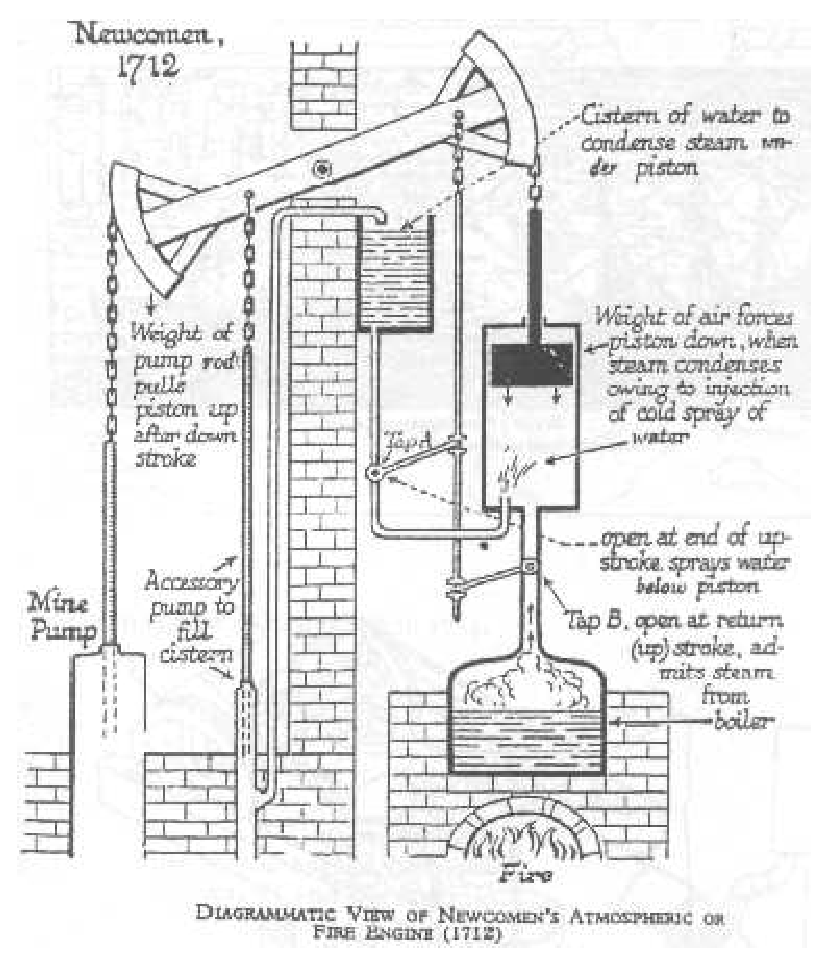
\includegraphics[height=14.0cm]{ambsthermopict/newcdiag} 
} 
\caption{Converting heat to kinetic (mechanical) energy in 1712.}
\label{heatmechanicalenergy} 
\end{figure}


\section{The Mystery of the 2nd Law}

The depth of confusion the 2nd Law has caused in the physics community
was recorded by Arnold Sommerfeld (1868--1951):

\begin{quote}\itshape
Thermodynamics is a funny subject. The first time you go through it,
you don't understand it at all. The second time you go through it, you
think you understand it, except for one or two small points. The third
time you go through it, you know you don't understand it, but by that
time you are so used to it, it doesn't bother you any more.
\end{quote}

The 2nd Law states that entropy cannot decrease with time, and when
strictly increasing characterises an \emph{irreversible} process,
defining an \emph{Arrow of Time}. Max Planck (1858--1947) located the
entire weight of the law in this irreversibility:

\begin{quote}\itshape
Were it not for the existence of irreversible processes, the entire
edifice of the 2nd Law would crumble.
\end{quote}

The mystery is that Newtonian deterministic mechanics \emph{without}
viscosity, like quantum mechanics, is formally time-reversible: the basic
equations are invariant under $t \to -t$. Mechanics \emph{with} viscosity
is obviously irreversible --- viscosity smooths gradients, an irreversible
operation. The question that haunted Maxwell, Boltzmann, Planck, Mach,
Ostwald and Prigogine was: how can a macroscopic system, whose
microscopic mechanics is reversible, exhibit macroscopic irreversibility?

Boltzmann took on the challenge and proposed \emph{statistical
mechanics}: an assumption of \emph{molecular chaos}, a microscopic game
of roulette that introduces an irreversible smoothing \emph{by
assumption}. The objection raised already by Loschmidt and re-stated by
Eisenschitz in 1958 was that this only shifts the question rather than
answering it:

\begin{quote}\itshape
The irreversible nature of the approach to equilibrium is apparently
incompatible with the reversibility of molecular dynamics. In resolving
this paradox the theory faces difficulties that have not yet been fully
overcome.
\end{quote}

This volume takes a different route. The 2nd Law, read in the
deterministic continuum framework, expresses the \emph{necessary
presence of turbulence arising from instabilities in slightly viscous
flow}. The adjective \textbf{slightly viscous} is central. In purely
inviscid flow there is no small-scale dissipation mechanism at all,
and no 2nd Law in the dissipative sense. In strongly viscous flow the
viscosity smooths the velocity field before instabilities can grow,
the flow stays laminar, and again no turbulence and no irreversible
dissipation. It is only in the \emph{slightly viscous} regime ---
viscosity small enough that the flow is unstable to the perturbations
inevitably present, but non-zero so that the resulting turbulent
cascades terminate by dissipation at the small scales --- that
instabilities grow into turbulence and turbulence necessarily generates
positive dissipation. The 2nd Law is the inevitability of this chain:
\begin{center}
\textbf{slightly viscous flow $\longrightarrow$ instabilities
$\longrightarrow$ turbulence $\longrightarrow$ dissipation $D > 0$.}
\end{center}
The chain is realised computationally by RNS as a finite-precision
solver for the deterministic continuum equations of compressible flow,
which automatically introduces the slight viscosity at the resolved
scale through its least-squares stabilisation. The next sections show
how, and the chapters that follow develop the consequences.

\section{Expansion Cools, Compression Warms}\label{sec:expansion_cools}

A second physical primitive of compressible flow, on which every
thermodynamic device in this volume rests, comes directly from the
internal-energy equation of a compressible gas. That equation contains
the \emph{pressure-work} term
\begin{equation}
  -\,p\,\nabla\!\cdot u,
  \label{eq:pdivu}
\end{equation}
whose sign tells the whole story:

\begin{itemize}
\item \textbf{Expanding flow} ($\nabla\!\cdot u > 0$, gas spreading
out): pressure work is negative, internal energy decreases, and the
gas \emph{cools}.
\item \textbf{Compressing flow} ($\nabla\!\cdot u < 0$, gas being
squeezed): pressure work is positive, internal energy increases, and
the gas \emph{warms}.
\end{itemize}

Cooling appears only in expanding flow; warming appears only in
compressing flow. The reverse never happens. This is the
thermodynamic primitive that, played out in different geometries,
produces every device of classical thermodynamics: Joule's free
expansion (Chapter~\ref{ch:joule}) realises the expansion-cools half
in one chamber and the compression-warms half in the other; the
refrigeration cycle (Chapter~\ref{ch:refrig}) exploits the same
asymmetry sustained by external work; the heat engine
(Chapter~\ref{ch:piston}) extracts useful work from the
compression-warms half of the cycle. The viscous dissipation
$\mu_{\mathrm{mom}}|\nabla u|^2 \geq 0$ that appears alongside the
pressure work in the energy equation is the irreversible floor of the
previous section --- the piece no real flow can avoid.

Packaged as global rates, writing $K$ for total kinetic energy, $E$
for total internal (heat) energy, $W = \int p\,\nabla\!\cdot u\,dx$
for the rate of pressure work, and $D = \int
\mu_{\mathrm{mom}}|\nabla u|^2\,dx \geq 0$ for the cumulative
dissipation rate, the two budgets read
\begin{equation}\label{eq:2nd_law_compact}
  \dot K \;=\; W - D, \qquad \dot E \;=\; -W + D,
\end{equation}
with total energy conservation $\dot K + \dot E = 0$ in the absence
of external heating. The pressure work $W$ runs in both directions
(expansion converts $E$ into $K$; compression converts $K$ into $E$);
the dissipation $D \geq 0$ runs only one way (always $K \to E$, never
the reverse). When you rub your hands they get warm, but heating your
hands does not produce the rubbing --- motion generates heat by
friction, heat does not generate motion by an inverse friction. The
classical 2nd Law is this asymmetry of $D$; the computational
restatement, developed in the chapters that follow, is that no
finite-precision solver of the deterministic continuum equations can
make $D$ vanish, because no pointwise solution of the Euler equations
exists in the turbulent/shock regime to which the deterministic
dynamics inevitably leads.

 \section{Turbulence}

There is another fundamental problem in science, namely the problem of \emph{turbulence} in a gas or fluid seen as a large collection of gas/fluid particles or atoms/molecules interacting by pressure and friction forces. Turbulent flow is not deterministic as concerns pointwise values in space and time, and thus has been approached by statistical methods, however with meager concrete results.

There are thus two main open problems of fluid dynamics:
\begin{itemize}
\item the 2nd Law and physical meaning of entropy,
\item mathematical modeling of turbulence, 
\end{itemize}
which have not been found a resolution within a deterministic framework, and to be honest not really within a statistical framework either as evidenced in quotations below. 
\newline
\indent
But there is midway between full determinism and full indeterminism or statistics, which we explored in 
our previous book \emph{Computational Turbulent Incompressible Flow} \cite{ambsflow}. We showed that mean-value quantities such as drag and lift in turbulent bluff body flow, can be computed deterministically without resort to statistics by \emph{Real Navier--Stokes} (RNS) from first principles of conservation of mass, momentum and
internal energy. RNS is the computational realisation of slightly viscous compressible flow by a least squares stabilised finite element method, which can be seen as a viscosity solution of the Navier--Stokes equations.
%solving the Euler/Navier-Stokes equations by a certain computational method named \emph{RNS} as an acronym for
\newline
\indent
RNS opens to an exploration of turbulent flow viewing RNS as direct model of physics with an automatic turbulence model emerging by computing best possible 
solutions to Euler's equations including \emph{turbulent dissipation} from least squares stabilisation. 
%RNS thus resolves the problem of turbulence in the sense of offering a computable understandable mathematical model 
RNS shows to satisfy a certain 2nd Law formulated without the concept of entropy, using only the known concepts of heat energy, kinetic energy, work together with turbulent dissipation, and thus offers a resolution of the problem of formulating a 2nd Law in physical terms. 
\newline
\indent
RNS essentially replaces entropy by turbulent dissipation and the 2nd Law comes out simply as a consequence of the inevitable presence of turbulent dissipation in certain processes.
\newline
\indent
RNS thus opens to a resolution of the two main open problems of mathematical modeling of turbulence and the 2nd Law,
by showing that the problems are essentially the same and can approached by deterministic computation. 

\section{ThermoDynamics}

\emph{Real Navier--Stokes} (RNS) is the \textbf{computational realisation of
slightly viscous compressible flow by a least squares stabilised finite
element method, which can be seen as a viscosity solution of the
Navier--Stokes equations}. In this book we use RNS in this sense as
\emph{Real Thermodynamics}: an exploration of basic processes of
thermodynamics --- heat engines, heat pumps and refrigerators --- in which
turbulent dissipation, generated automatically by the least-squares
stabilisation at the resolved scale, sets the \emph{limits of process
efficiency}.

In the spirit of Dijkstra~\cite{dijkstra}, RNS is taken here as the
physical model of thermodynamics --- the Euler equations
\emph{together with} a computational solution procedure, not the Euler
equations on their own without a constructive way of solving them.
The shift this enforces is methodological: turbulent and shock
solutions are no longer objects to be reasoned about a priori but
objects to be computed and inspected a posteriori. Mean-value outputs
of those computed solutions --- drag, lift, total dissipation $D$ ---
turn out to be stable under perturbations of the discretisation;
point-values do not. Chapter~\ref{ch:new_foundation} develops the
duality argument by which this wellposedness can be checked case by
case from the computed RNS solution itself.

RNS is realised in simple geometry in short \emph{Claude Codes} hosted on the
GitHub repository \texttt{github.com/Claes542/RealMolecule}, intended to be
run in parallel with the text: each conceptual chapter has a companion
browser-runnable simulation (\texttt{joule\_experiment\_cpu.html},
\texttt{piston\_cylinder\_cpu.html}, \texttt{cosmology\_2d\_cpu.html}, \ldots)
in which the reader can vary parameters, watch the dissipation $D$ accumulate
in real time, and verify the argument of the text directly. Each code is
short --- a few hundred lines of self-contained HTML/JavaScript including the
canvas drawing, sliders and diagnostics --- so the reader can \textbf{scan
the whole simulation code in fifteen minutes} and see exactly how the
deterministic continuum equations and the least-squares stabilisation are
implemented, with no library, build step or installation in between.


\iffalse  % --- essentials merged into Ch. 1 "The Mystery of the 2nd Law" section ---
\chapter{The Mystery of the 2nd Law}

\small



\begin{quote} You can fool all the people some time, 
and some of the people all the time, but you cannot fool
all people all the time. (Abraham Lincoln)
\end{quote}
\normalsize



The physicist Arnold Sommerfeld (1868-1951) gave the 
following account of his experience of thermodynamics 
as a scientific discipline:
\begin{itemize}
\item  
\emph{Thermodynamics is a funny subject. The first time you go through it, 
you don't understand it at all. The second time you go through it, you 
think you understand it, except for one or two small points. 
The third time you go through it, you know you don't understand it, 
but by that time you are so used to it, it doesn't bother you any more.} 
\end{itemize}
The greatest mystery is the \emph{2nd 
Law of Thermodynamics}, which has haunted
many great scientists into obsession including Maxwell, Boltzmann,
Planck, Mach, Ostwald and Prigogine, ever since it was formulated in 1865 by
Clausius.

The 2nd Law states that a certain quantity named \emph{entropy} 
cannot decrease with increasing time, and when strictly increasing 
characterizes an \emph{irreversible} thermodynamic process, 
which cannot be reversed in time, since the reversed process would
have a strictly decreasing entropy violating the 2nd Law.
A direction of time or \emph{Arrow of time} would thus be defined by 
irreversible thermodynamics.
%The classical 2nd Law states that the entropy cannot decrease with increasing time; 
%it may stay constant or it may increase,
%but it can never decrease (for an isolated system) in forward time. 
%A process with $dS>0$ is irreversible in time, because the reversed 
%process would have $dS<0$ violating the 2nd Law.
Max Planck (1858-1947) expressed the role of the 2nd Law as follows: 
%\cite{planck1,planck2,planck3}: 
\begin{itemize}
\item \emph{Were it not for the 
existence of irreversible processes, the entire edifice
of the 2nd Law would crumble}.
\end{itemize}
Newtonian deterministic mechanics \emph{without} viscosity/friction, 
as well as quantum 
mechanics, is formally time reversible, since the basic equations are invariant
under time reversal, and Planck pointed to the need of  
explaining how irreversibility can arise in a formally reversible 
deterministic system,  more precisely how it can be that
a \emph{macroscopic} process based on reversible \emph{microscopic} mechanics, 
can be irreversible.

Newtonian mechanics \emph{with} slight viscosity 
from microscopic viscosity, is easily seen to be irreversible 
as a consequence of the smoothing effect of viscosity;  
it is of course not surprising that a processes \emph{with} viscosity 
shows effects \emph{of} viscosity. What physicists of the 
late 19th century were asking was 
\emph{how} effects of friction/viscosity can
arise in a macroscopic system based on reversible microscopic
particle/quantum mechanics \emph{without} viscosity.
  
Ludwig Boltzmann (1844-1906) took on the challenge and came up with
a resolution in the  form of \emph{statistical mechanics} based on 
an assumption of \emph{molecular chaos}, or molecular games of roulette, 
supposedly reflecting a tendency of thermodynamical processes
to evolve from \emph{ordered} towards \emph{disordered} states, 
or from \emph{less probable} towards \emph{more probable} states, 
identified by increasing entropy.
But a molecular game of roulette introduces a microscopic viscous effect 
\emph{by assumption}, and thus is similar to deterministic
mechanics \emph{with} microscopic viscosity with the same lack of 
explicative power of irreversibility, as noted in early criticism by Loschmidt
\cite{loschmidt} and expressed by Eisenschitz in the introduction of his 
\emph{Statistical Theory of Irreversible Processes} from 1958:
\begin{itemize}
\item \emph{The irreversible nature of the approach to
equilibrium is apparently incompatible with the reversibility
of molecular dynamics. In resolving this paradox the theory
faces difficulties that have not yet been fully overcome}.
\end{itemize} 
Further, observations of \emph{self-organization} and \emph{emergence} 
of order out of chaos contradict steady
increase of disorder/entropy. 
Nevertheless, in the absence of a better explanation,
statistical mechanics is today viewed by the physics community as the 
foundation of thermodynamics offering a justification 
of both the 2nd Law, irreversibility 
and the Arrow of time. But statistical mechanics is difficult 
to understand
and to use: The modern text-book \cite{laurendau} 
prepares the student for (very) tough studies:
\begin{itemize}
\item \emph{Statistical thermodynamics is a challenging discipline...
It demands an incredible diversity of skills, from probability theory
to quantum mechanics to molecular modeling...transport phenomena
and physical optics. With continuing study
and reflection you can rest assured that a practical symbiosis will
eventually bloom that simultaneously reinforces and expands your
appreciation of both microscopic and macroscopic thermodynamics}.
\end{itemize}
   

The objective of this book is to 
develop a deterministic foundation of thermodynamics in the form of
\emph{computational thermodynamics}, which does not rely on any form of 
statistical mechanics. We show that
computational thermodynamics offers accurate simulation
and scientific understanding of complex real thermodynamical processes,
without requiring any ``incredible diversity of skills''. In short,
we show that thermodynamics can be made both understandable and applicable.
The basic idea is to view physical processes 
as some form of \emph{finite precision analog computation}, 
which can be simulated by \emph{finite precision digital computation}.


We shall see  that computational thermodynamics opens new possibilities 
to progess with new questions and answers, in particular concerning 
the phenomena of \emph{turbulence} and \emph{shocks} typically occuring
in the thermodynamics of slightly viscous flow dominating applications.
The basic novelty is that turbulent/shock solutions are computed and thus 
are available to inspection, which means that the focus of the science
of thermodynamics can be shifted from \emph{a priori} predictions 
based on analytical mathematics to \emph{a posteriori} analysis of 
computed turbulent solutions, which can be viewed as a 
veritable shift of paradigm.

The new computational foundation is based on a 
\emph{1st Law of Thermodynamics} in the form of 
the \emph{Euler equations of an ideal gas} 
expressing \emph{conservation of mass, momentum and energy},
combined with \emph{finite precision computation} in the form of
a \emph{least squares stabilized finite element method} 
referred to as \emph{RNS}.
We prove a \emph{2nd Law of Thermodynamics} without the concept entropy 
to be a consequence of the 1st Law combined with finite precision computation.

With a 2nd Law in this form we avoid the (difficult) main task of 
statistical mechanics of specifying the physical significance of 
entropy and motivating its tendency to increase by probabilistic 
considerations based on (tricky) combinatorics. Yet, we achieve the
main goal of the 2nd Law of giving a rational expression
and explanation of irreversibility in macroscopic systems based on formally
reversibe microscopic mechanics.
Thus using \emph{Ockham's razor} \cite{ockham},
we rationalize a scientific theory of major importance making it both
more understandable and more useful. The new 2nd Law is closer to 
classical Newtonian mechanics than the 2nd Law of statistical mechanics, 
and thus can be viewed to be more fundamental.

We shall see that RNS is not just any ad hoc computational method for the
Euler equations, but is designed to capture the fundamentals of thermodynamics
including turbulence and shocks.
We will thus view RNS as a constructive physical model of thermodynamics, in distinction
from a classical non-constructive mathematical model
without computational solution procedure.

A fundamental question concerns \emph{wellposedness} in the sense
of Hadamard, that is what aspects or \emph{outputs} of turbulent/shock 
solutions are \emph{stable} under perturbations, that is what outputs change
little under small perturbations including perturbations from the
computational discretization and mesh. 
We show that wellposedness of RNS solutions
can be tested a posteriori by computationally solving a \emph{dual linearized
problem}, through which the output sensitivity of non-zero Euler residuals
can be estimated. We find that mean-value outputs such as drag and lift 
and total turbulent dissipation are wellposed, while point-values
of turbulent flow are not. We can thus a posteriori case by case assess 
the quality of RNS solutions as solutions of the Euler equations. 

%But
%we refrain from the seemingly hopeless task of proving a priori that  
%RNS will produce a wellposed solution for all data, (even without 
%computing the solution).    


%The \emph{2nd Law} for RNS is formulated in terms of  
%the basic physical quantities of \emph{kinetic energy}
%$K$, \emph{heat energy} $E$, rate of \emph{work} $W$ and 
%\emph{shock/turbulent dissipation}
%$D>0$, and takes the form:
%\begin{equation}\label{secondlaw0}
%\dot K=W-D,\quad \dot E=-W+D,
%\end{equation}
%where the dot indicates time differentiation. Slightly viscous
%flow always develops shocks/turbulence with $D>0$, and the  
%2nd Law thus expresses an irreversible transfer of kinetic energy
%into heat energy, while the total energy $E+K$ remains constant.







   
\fi  % --- end merged-into-Ch.1 block ---

\chapter{Classical Thermodynamics}
\small
\begin{quote} Heat, a quantity which functions to animate, derives
from an internal fire located in the left ventricle. (Hippocrates, 460 B.C.)
\end{quote}
%\begin{quote}
%Those who have talked of ``chance'' are the
%inheritors of antique superstition and ignorance...whose minds have never
%been illuminated by a ray of scientific thought. (T. H. Huxley)
%\end{quote}
\normalsize 

%\section{FEniCS as Computational Science}

%The goal of the FEniCS project is to develop software for automated computational solution of differential equations based on 
%a finite element methodology combining generality with efficiency. 
%The FEniCS Application Unicorn offers a 
%solver for a fluid-solids continuum based on a unified Eulerian formulation of momentum balance combined with constitutive laws for 
%fluid/solid in Eulerian/updated Lagrangian form, which shows the capability of FEniCS for automation of 
%computational fluid-structure interaction. 
%Thermodynamics is a basic area of continuum mechanics with many important applications, which however is feared 
%by both teachers, students and engineers as being difficult to understand and to apply, principally because of the %apperance of turbulence. 
%In this article we show that turbulent thermodynamics can be made understandable and useful by automated 
%computational solution, as a demonstration of the capability of FEniCS. 

%The biggest mystery of classical thermodynamics is the 2nd Law about entropy and automation 
%cannot harbor any mystery. 
%Expert systems are required for mysteries and FEniCS is not an expert system.
%Automation requires a continuum mechanics formulation of thermodynamics with a transparent 2nd Law.
%We present a formulation of thermodynamics based on finite precision computation with a 2nd Law without
%reference to entropy, which we show can serve as a basis for automated computational simulation of complex turbulent thermodynamics
%and thus can open to new insight and design, a main goal of FEniCS. In this setting the digital finite element model becomes the 
%real model of the physics of thermodynamics viewed as a form of analog finite precision computation, a model which is open to 
%inspection and analysis because solutions can be computed and put on the table. This represents a new kind of science in the 
%spirit of Dijkstra \cite{dijkstra} and Wolfram \cite{wolfram}, which can be explored using FEniCS and which we present in non-technical form in My Book of Knols \cite{knol}.     


\section{Classical 1st and 2nd Laws}

\emph{Thermodynamics} is fundamental in a wide range of phenomena from
macroscopic to microscopic scales. 
Thermodynamics essentially concerns the interplay between \emph{heat energy} 
and \emph{kinetic energy} in a \emph{gas} or \emph{fluid}. 
Kinetic energy, or \emph{mechanical energy}, 
may generate heat energy by 
\emph{compression}
or \emph{turbulent dissipation}. 
Heat energy may generate kinetic energy by \emph{expansion}, but
not through a \emph{reverse} process of turbulent dissipation. 
The industrial society
of the 19th century was built on the use of \emph{steam engines}, and the 
initial motivation to understand thermodynamics came from a need to
increase the efficiency of steam engines for conversion of heat energy to
useful mechanical energy. 
Thermodynamics is closely connected to the dynamics of \emph{slightly viscous}
and \emph{compressible} gases, since substantial compression and 
expansion can occur in a gas, but less in fluids (and solids).

The development of classical thermodynamics as a rational science 
based on logical deduction from a set of axioms, was initiated in 
the 19th century by Carnot \cite{carnot}, Clausius 
\cite{clausius} and Lord Kelvin \cite{kelvin}, who formulated
the basic axioms in the form of the \emph{1st Law} and the \emph{2nd Law} of
thermodynamics. The 1st Law states (for an isolated system)
that the \emph{total energy},
the sum of kinetic and heat energy, is conserved.
The 1st Law is naturally generalized to include also conservation 
of mass and Newton's law of conservation of momentum and then 
can be expressed as the \emph{Euler equations} for  a gas/fluid 
with \emph{vanishing viscosity}.
%The 1st law can be viewed as a definition, with any loss of kinetic 
%energy defined to be heat energy. 

The 2nd Law has the form of an inequality 
$dS\ge 0$ for a quantity
named \emph{entropy} denoted by
$S$, with $dS$ denoting change thereof, supposedly  
expressing a basic feature of real thermodynamic processes.
The classical 2nd Law states that the entropy cannot decrease; 
it may stay constant or it may increase,
but it can never decrease (for an isolated system). 

The role of the 2nd Law is
to give a scientific basis to the many observations  
of \emph{irreversible} processes, that is, processes which cannot 
be reversed in time, like running a movie backwards. 
Time reversal of a 
process with strictly increasing entropy, would correspond
to a process with strictly 
decreasing entropy, which would violate the 2nd Law and therefore could
not occur. A perpetum mobile would represent a reversible
process and so the role of the 2nd Law is in particular to explain \emph{why}
it is imposssible to construct a perpetum mobile, and
\emph{why} time is moving forward in the direction an
\emph{arrow of time}, as expressed by  Max Planck 
\cite{planck1,planck2,planck3}: \emph{Were it not for the 
existence of irreversible processes, the entire edifice
of the 2nd Law would crumble}.

While the 1st Law in the form of the Euler equations
expressing conservation of mass, momentum and total energy
can be understood and motivated on rational grounds, 
the nature of the 2nd Law is mysterious.
It does not seem to be a consequence of the 1st Law, since the Euler
equations seem to be time reversible, and the role of the 2nd Law is to 
explain irreversibility. We repeat the questions from above since they are so central: 
\begin{itemize}
\item
If the 2nd Law is a new independent law of 
Nature, how can it be justified? 
\item What is the physical significance of that quantity named entropy, 
which Nature can only get more of and never can get rid of, like 
a steadily accumulating heap of waste? 
\item What mechanism prevents Nature from recycling entropy? 
\item How can irreversiblity arise in a reversible system? 
\item How can viscous dissipation arise in a 
system with vanishing viscosity? 
%\item Why is there no \emph{Maxwell demon} \cite{maxwell}? 
\item Why can a gas by itself expand
into a larger volume, but not by itself contract back again,
if the motion of the gas molecules is governed by the reversible Newton's
laws of motion? 
\item Why is there an arrow of time? 
\end{itemize}
%This article presents answers.

  


%\begin{figure}[bhpt] 
%\centerline{ 
%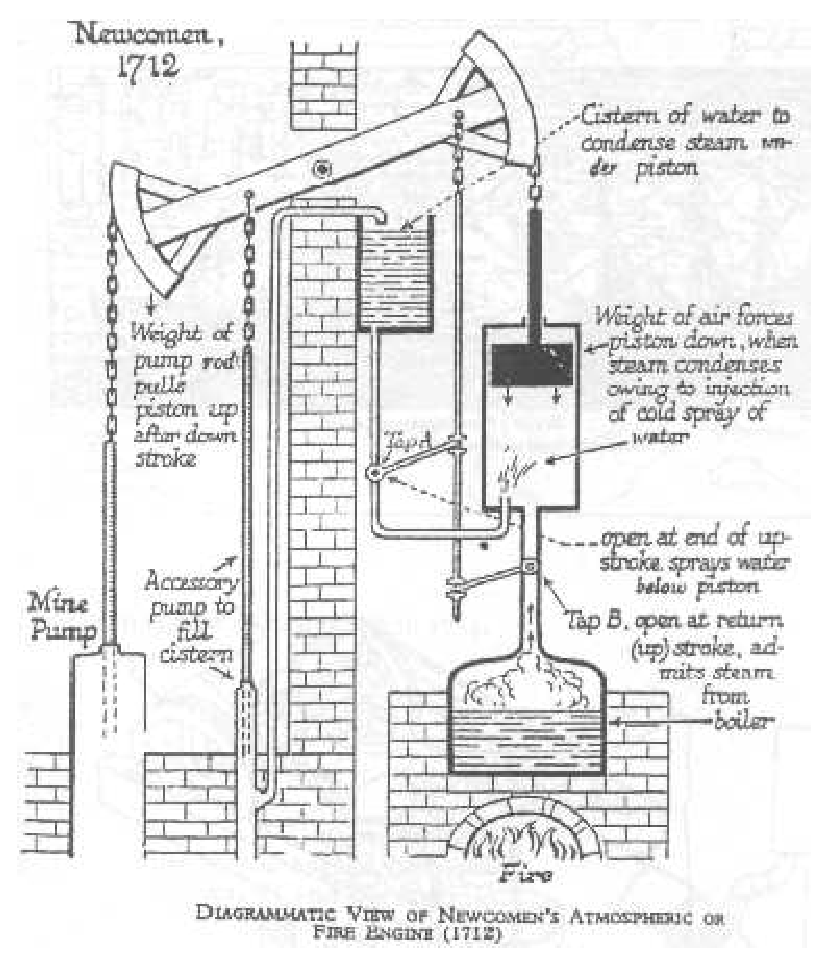
\includegraphics[height=12.0cm]{ambsthermopict/newcdiag.eps} 
%} 
%\caption{Converting heat to kinetic (mechanical) energy in 1712.}
%\label{nse_people} 
%\end{figure}

\section{The Mystery of Entropy}

These were the questions which confronted scientists 
in the late 19th century, after the introduction  of the concept of entropy
by Clausius in 1865, and these showed to be tough questions to answer.
After much struggle, agony and debate, the agreement of the 
physics community has become to  
view \emph{statistical mechanics} based on an
assumption of \emph{molecular chaos} as developed by Boltzmann 
\cite{boltzmann}, 
to offer a rationalization of the classical 2nd Law in the form
of a tendency of (isolated) physical processes to move from improbable towards 
more probable states, or from ordered to less ordered states.

Boltzmann's assumption of molecular chaos in a dilute gas of colliding
molecules, is that two molecules about to collide have
independent velocities, which led to the \emph{H-theorem} 
for \emph{Boltzmann's equations} stating that a certain quantity
denoted by $H$ could not decrease and thus could serve as
an entropy defining an arrow of time.
 
Increasing disorder would thus represent increasing entropy, and the
classical 2nd Law would reflect the eternal pessimistists idea that things 
always get more messy, and 
that there is really no limit to this,
except when everything is as messy as it can ever get. Of course, experience
could give (some) support this idea, but the trouble is that it prevents things
from ever becoming less messy or more structured, and 
thus may seem a bit too pessimistic.

No doubt, it would seem to contradict the many observations of 
\emph{emergence} of ordered non-organic structures (like crystals or
waves and cyclons) and organic structures (like DNA and human beings), 
seemingly out of disordered chaos, as evidenced by the physics
Nobel Laureate Robert Laughlin \cite{laughlin}.

%\begin{figure}[bhpt] 
%\centerline{ 
%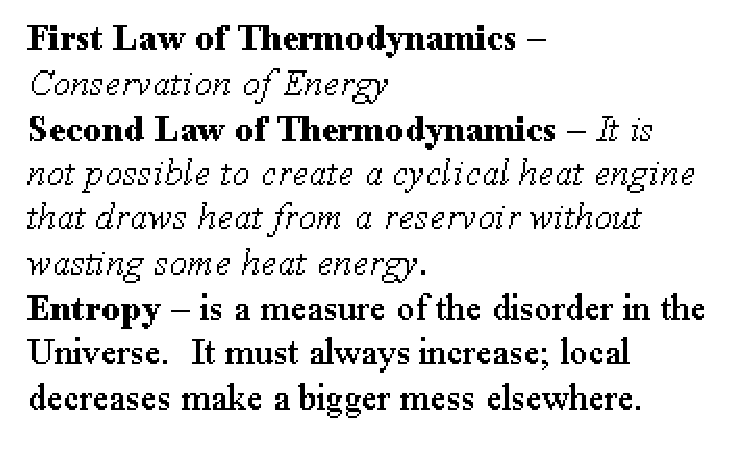
\includegraphics[height=6.0cm]{ambsthermopict/lawsofthermodynamics.eps} 
%} 
%\caption{Classical thermodynamics in a nutshell (from the web).}
%\label{nse_people} 
%\end{figure}

Most trained thermodynamicists
would here say that emergence of order
out of chaos, in fact does not contradict the classical 2nd Law, 
because it concerns 
``non-isolated systems''. But they would probably insist that  
the Universe as a whole (isolated system) would steadily evolve towards a   
``heat-death'' with maximal entropy/disorder (and no life), thus
fulfilling the pessimists expectation. The question from where the
initial order came from, would however be left open.

The standard presentation of thermodynamics based on the 
1st and 2nd Laws, thus involves a mixture of deterministic 
models (Boltzmann's equations with the H-theorem) based on
statistical assumptions (molecular chaos) making the subject
admittedly difficult to both learn, teach and apply, 
despite its strong importance. 

This is primarily because the question \emph{why} necessarily $dS\ge 0$ and never $dS<0$, is not
given a convincing understandable answer. 
In fact, statistical mechanics allows 
$dS<0$, although it is claimed to be very unlikely. The basic objective
of statistical mechanics as the basis of classical thermodynamics,
thus is to (i) give the entropy a physical meaning, and (ii) to motivate
its tendency to (usually) increase. 

Before statistical mechanics,
the 2nd Law was viewed as an experimental fact, which could not
be rationalized theoretically. The classical view on the 2nd Law
is thus either as a statistical law of large numbers or as a an 
experimental fact, both without a rational deterministic mechanistic 
theoretical foundation. The problem with thermodynamics in this form
is that it is understood by very few, if any, as indicated by the above quotes.

%\small
%\begin{itemize}
%\item \emph{Every mathematician knows it is impossible to understand
%an elementary course in thermodynamics.} (V. Arnold)
%\item \emph{...no one knows what entropy is, so if you in a debate use
%this concept, you will always have an advantage.} (von Neumann to Shannon)
%\item \emph{As anyone who has taken a course in thermodynamics is well aware,
%the mathematics used in proving Clausius' theorem (the 2nd Law) is of a very
%special kind, having only the most tenous relation to that known to
%mathematicians.} (S. Brush \cite{brush})
%\item \emph{Where does irreversibility come from? It does not come
%form Newton's laws. Obviously there must be some law, some
%obscure but fundamental equation. perhaps in electricty,
%maybe in neutrino physics, in which it does
%matter which way time goes.} (Feynman \cite{feynman})
%\item
%\emph{For three hundred years science has been dominated by 
%a Newtonian paradigm presenting the World either
%as a sterile mechanical clock or in a state of degeneration 
%and increasing disorder...It has always seemed paradoxical
%that a theory based on Newtonian mechanics can lead
%to chaos just because the number of particles is large, 
%and it is subjectivly decided that their precise motion cannot be 
%observed by humans... In the Newtonian world of necessity, there
%is no arrow of time. Boltzmann found an arrow hidden in  
%Nature's molecular game of roulette.}
%(Paul Davies \cite{davies})
%\item \emph{The goal of deriving the law of entropy increase
%from statistical mechanics has so far eluded the deepest
%thinkers.} (Lieb \cite{lieb})
%\item \emph{There are great physicists who have not understood it}.
%(Einstein about Boltzmann's statistical mechanics) 
%\end{itemize}
%\normalsize

\chapter{What Scientists Confess About Thermodynamics}

To motivate the that thermodynamics needs a new foundation, we here collect some of the many 
expresssions in the literature giving evidence that classical thermodynamics is a mess:


\begin{itemize}
\item \emph{Every mathematician knows it is impossible to understand
an elementary course in thermodynamics.} (V. Arnold)
\item \emph{...no one knows what entropy is, so if you in a debate use
this concept, you will always have an advantage.} (von Neumann to Shannon)
\item \emph{As anyone who has taken a course in thermodynamics is well aware,
the mathematics used in proving Clausius' theorem (the 2nd Law) is of a very
special kind, having only the most tenous relation to that known to
mathematicians.} (S. Brush \cite{brush})
\item \emph{Where does irreversibility come from? It does not come
form Newton's laws. Obviously there must be some law, some
obscure but fundamental equation. perhaps in electricty,
maybe in neutrino physics, in which it does
matter which way time goes.} (Feynman \cite{feynman})
\item
\emph{For three hundred years science has been dominated by 
a Newtonian paradigm presenting the World either
as a sterile mechanical clock or in a state of degeneration 
and increasing disorder...It has always seemed paradoxical
that a theory based on Newtonian mechanics can lead
to chaos just because the number of particles is large, 
and it is subjectivly decided that their precise motion cannot be 
observed by humans... In the Newtonian world of necessity, there
is no arrow of time. Boltzmann found an arrow hidden in  
Nature's molecular game of roulette.}
(Paul Davies \cite{davies})
\item \emph{The goal of deriving the law of entropy increase
from statistical mechanics has so far eluded the deepest
thinkers.} (Lieb \cite{lieb})
\item \emph{There are great physicists who have not understood it}.
(Einstein about Boltzmann's statistical mechanics) 
\item  \emph{...thermodynamics is a dismal swamp of obscurity...
a prime example to 
show that physicists are not exempt from the madness
of crowds...\\
Clausius' verbal statement of the second law makes 
no sense...All that remains is a Mosaic prohibition; 
a century of philosophers and journalists have acclaimed this 
commandment; a century of mathematicians have shuddered and
averted their eyes from the unclean...Seven times in the past thirty 
years have I tried to follow the argument Clausius
offers and seven times has it blanked and gravelled me. I cannot
explain what I cannot understand}. (Truesdell \cite{truesdell})
\item \emph{The second law of thermodynamics is, without a doubt, one of 
the most perfect laws in physics. Any reproducible violation of it, however 
small, would bring the discoverer great riches as well as a trip to Stockholm. 
The world's energy problems would be solved at one stroke. It is not 
possible to find any other law (except, perhaps, for super selection rules 
such as charge conservation) for which a proposed violation would bring more 
skepticism than this one. Not even Maxwell's laws of electricity or 
Newton's law of gravitation are so sacrosanct, for each has measurable 
corrections coming from quantum effects or general relativity. The law 
has caught the attention of poets and philosophers and has been called t
he greatest scientific achievement of the nineteenth century. Engels 
disliked it, for it supported opposition to Dialectical Materialism, 
while Pope Pius XII regarded it as proving the existence of a higher being.}
(Bazarov in \emph{Thermodynamics}, 1964)

\item \emph{If someone points out to you that your pet theory of the universe is in 
disagreement with Maxwell's equations, then so much the worse for 
Maxwell's equations. If it is found to be contradicted by observation, well, 
these experimentalists do bungle things sometimes. But if your theory 
is found to be against the second law of thermodynamics I can give you 
no hope; there is nothing for it but to collapse in deepest humiliation}
(Sir Arthur Stanley Eddington in \emph{The Nature of the Physical 
World}, 1915)
\item \emph{A good many times I have been present at gatherings of people who, 
by the standards of the traditional culture, are thought highly educated 
and who have with considerable gusto been expressing their incredulity at 
the illiteracy of scientists. Once or twice I have been provoked and have 
asked the company how many of them could describe the Second Law of 
Thermodynamics. The response was cold: it was also negative.}
(C. P. Snow in 1959 Rede Lecture entitled 
\emph{The Two Cultures and the Scientific Revolution}).
\end{itemize}



\noindent
From \emph{Challenges to the 2nd Law of Thermodynamics} by V. Capek and D. P. Sheenan:

\noindent
\begin{itemize} 
\item \emph{This monograph is the first to examine modern challenges to the 2nd Law. For more than a century
this field has lain fallow and beyond the pale of legitimate scientific inquiry due to both a dearth of scientific results and to a surfeit of peer pressure against such inquiry}.
\item \emph{It is remarkable that 20th century physics, which embraced several radical paradigm shifts, was unwilling to wrestle with this remnant of 19th century physics, whose foundations were admittedly suspect and largely unmodified by the discoveries of the succeeding century}.
\item \emph{This failure is due in part to the many strong imprimaturs placed on it by prominent scientists like Planck, Eddington and Einstein. There grew around the second law a nearly inpentrable mystique which only now is being pierced}.
\item \emph{The 2nd Law has no general theoretical proof and, like all physical laws, its status is tied ultimately to experiments}.
\item \emph{Inquiry into its status should not be stifled by certain unscientific attitudes and practices that have operated thus far}.
\end{itemize} 

\noindent
From \emph{A History of Thermodynamics: The Doctrine of Energy and Entropy} by Ingo M\"uller:
\begin{itemize}
\item \emph{A physicist likes to be able to grasp his concepts plausibly and on an intutive level. In that respect, however, the entropy - for all its proven an recognized importance - is a disappointment. The formula $dS=\frac{dQ}{T}$ does not lend itself to a suggestive interpretation}.
\end{itemize}

\noindent
From \emph{Classical Thermodynamics as Theory of Heat Engines} by C. Truesdell and S. Bharatha:
\begin{itemize}
\item \emph{I do not think it s possible ton write a history of a science until that science itself shall have been understood, thanks to a clear, explicit, and decent logical structure. The exuberance of dim, involute, and undisciplined historical essays upon classical thermodynamics reflects the confusion of the theory itself}.
\item \emph{Thermodynamics was born in obscurity and disorder, not to say confusion, and there the common presentations of it has remained}.
\end{itemize}

\noindent
From \emph{Tragicomical History of Thermodynamics} by C. Truesdell:
\begin{itemize}
\item \emph{Thermodynamics is the kingdom also of running current history as well as polemics, not to mention verbosity.
In no other discipline have the same equations been published over and over again so many times by different authors in different ill-defined notations and therefore claimed as his own by each; in no other has a single author seen fit to publish essentially the same ideas over and over again within a perieod of twenty years; and nowhere is else is the ratio of talk and excuse  to reason and result so high...}
\end{itemize}


\chapter{The Statistical Programme: Boltzmann to Planck}
\small
\begin{quote}
Those who have talked of ``chance'' are the
inheritors of antique superstition and ignorance...whose minds have never
been illuminated by a ray of scientific thought. (T. H. Huxley)
\end{quote}
%\begin{quote}
%What we observe as material bodies and forces are nothing but shapes and 
%variations in the structure of space.
%Particles are just schaumkommen (appearances). ...
%Let me say at the outset, that in this discourse, I am opposing not a few 
%special statements of quantum physics held today (1950s), I am opposing 
%as it were the whole of it, I am opposing its basic views that have been 
%shaped 25 years ago, when Max Born put forward his probability 
%interpretation, which was accepted by almost everybody...
%I don't like it, and I'm sorry I ever had anything to do with it. 
%(Schr\"odinger \cite{schrodinger2})
%\end{quote} 
\normalsize


\section{The Enigma}
While the 1st Law in the form of conservation of
energy can be viewed as a definition of internal 
energy, and as such cannot be disputed, the nature of the 2nd Law 
posed a main challenge to the scientists 
of the late 19th century with the following basic questions: 
%after the introduction  of the concept of entropy
%by Clausius in 1865. 
%It does not seem to be a consequence of the 1st Law, which 
%seems to be time reversible, and the role of the 2nd Law is to 
%explain irreversibility. Thus questions are lining up:
\begin{itemize}
\item Is the 2nd Law a law of Nature which can be justified,
or is it an experimental fact beyond rationalization? 
\item What is the physical significance of that quantity named entropy, 
which Nature can only get more of and never can get rid of, like 
a steadily accumulating heap of waste? What mechanism prevents Nature 
from recycling entropy?
\item How can irreversibility arise in reversible mechanics?   
%\item How can irreversiblity arise in a 
%reversible system? 
%\item How can viscous dissipation arise in a 
%system with vanishing viscosity? 
%\item Why is there no \emph{Maxwell demon} \cite{maxwell}? 
%\item Why can a gas by itself expand
%into a larger volume, but not by itself contract back again,
%if the motion of the gas molecules is governed by the reversible Newton's
%laws of motion? 
%\item Why is there an arrow of time?
\end{itemize}
%\newpage
The enigma Boltzmann set out to solve was to explain \emph{how} 
in reversible mechanics there can be irreversible processes 
with an Arrow of time, and his solution was 
``Nature�s molecular game of roulette''  or molecular chaos 
in a \emph{particle model} of a dilute gas of elastically colliding 
molecules, \emph{assuming} pairs of 
molecules about to collide 
to have statistically independent velocities \emph{before} collision,
but not after. From the statistical particle model Boltzmann
derived a deterministic \emph{kinetic model} in the form
of \emph{Boltzmann's equation} for the particle density as 
a function of position, velocity and time as independent
variables. Boltzmann proved that solutions
satisfy a 2nd Law referred to as the \emph{H-theorem},
as a consequence of the assumption of molecular chaos. 
Boltzmann's solution was immediately heavily criticized, in particular  
by Loschmidt \cite{loschmidt}, who pointed to the (obvious)
fact that assuming statistical independence \emph{before} collision,
effectively defines an Arrow of time and thus assumes what is to
be demonstrated.  

\section{From Boltzmann to Planck}
In ``an act of despair'' Max Planck 
stimulated by statistical mechanics proposed to explain the irreversible 
nature of \emph{black-body radiation} in terms of statistics of 
light quanta, which initiated quantum mechanics. Boltzmann was annihilated 
by the criticism,
but not his atomic games of roulette, which became the signum
of the physics of the 20th century.

\section{Emergence}

However, the criticism remains into our days: Molecular games of roulette with steadily 
increasing disorder
is incompatible with \emph{emergence} of ordered structures (like crystals,
waves and cyclons or DNA and human beings), as pointed out
by many including the physics Nobel Laureate Robert 
Laughlin \cite{laughlin}. 

\section{Microscopics of Microscopics}

Microscopics of macroscopics in the 
form of games of roulette requires its own microscopics,
which leads to a neverending chain of microscopics upon microscopics.
Einstein and Schr\"odinger never accepted the statistical 
\emph{Copenhagen interpretation} of quantum mechanics forefully 
advocatd by in particular Nils Bohr, who dismissed their criticism 
as an early onset of senility. However, an (informal) poll taken at the 1997 
UMBC quantum mechanics workshop gave the Copenhagen interpretation 
less than half of the votes (http://space.mit.edu/home/tegmark/).

%with \emph{vanishing viscosity}.
%The 1st law can be viewed as a definition, with any loss of kinetic 
%energy defined to be heat energy. 

%\begin{figure}[bhpt] 
%\centerline{ 
%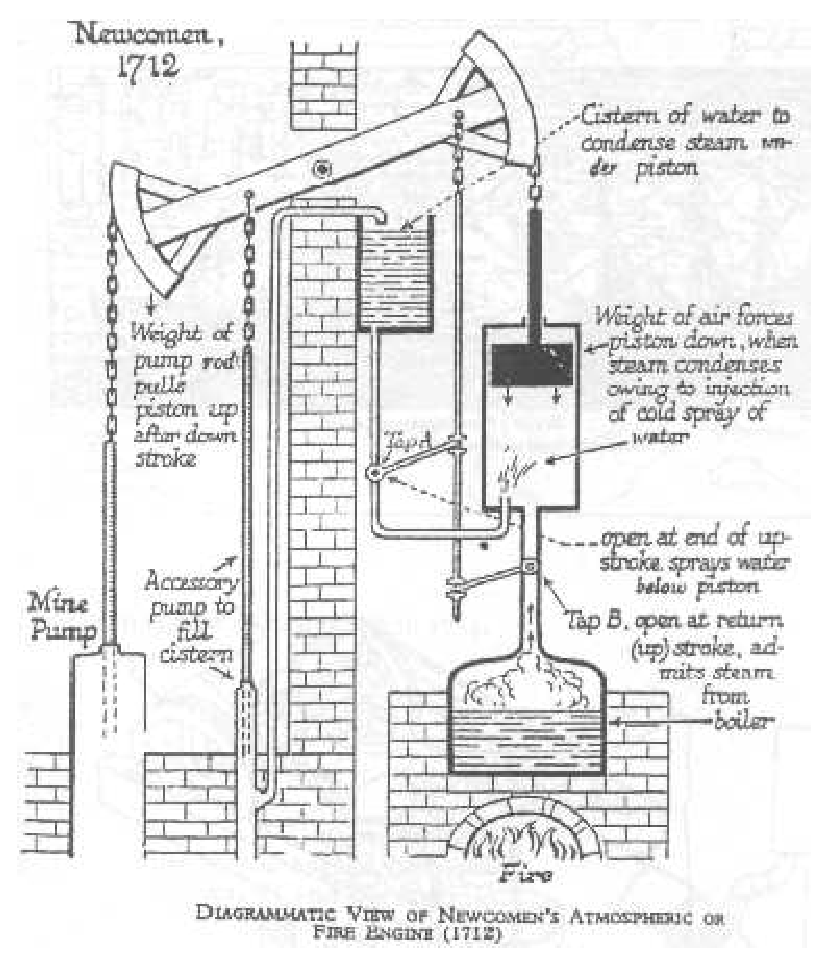
\includegraphics[height=12.0cm]{ambsthermopict/newcdiag.eps} 
%} 
%\caption{Converting heat to kinetic (mechanical) energy in 1712.}
%\label{nse_people} 
%\end{figure}

%After long debate the agreement of the 
%physics community has become to view \emph{statistical mechanics}
%developed by Boltzmann \cite{boltzmann} to offer a justification 
%of the classical 2nd Law as a tendency of many-particle 
%systems to move from less probable towards more probable states, 
%or from more ordered to 
%less ordered states. Statistical mechanics is based on an
%assumption of \emph{molecular chaos} 
%Increasing entropy would then represent increasing disorder  
%and the H-theorem would reflect the eternal pessimistists idea that things 
%always get more messy, and 
%that there is really no limit to this,
%except when everything is as messy as it can ever get. Of course, experience
%could give (some) support this idea, but the trouble is that it prevents things
%from ever becoming less messy or more structured, and 
%thus may seem a bit too pessimistic.



%\begin{figure}[bhpt] 
%\centerline{ 
%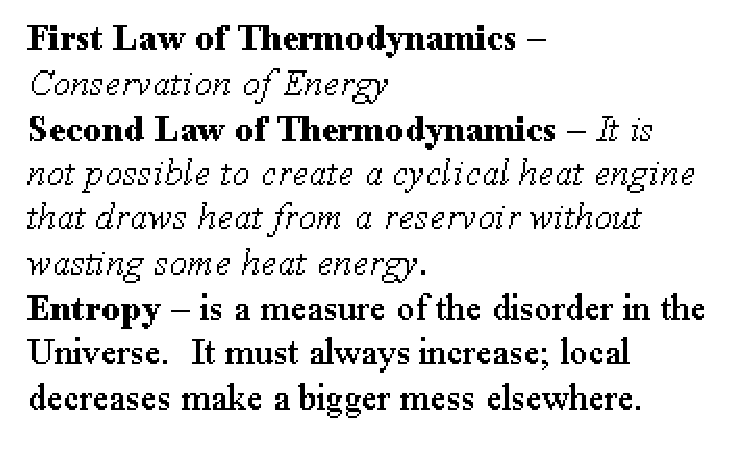
\includegraphics[height=6.0cm]{ambsthermopict/lawsofthermodynamics.eps} 
%} 
%\caption{Classical thermodynamics in a nutshell (from the web).}
%\label{nse_people} 
%\end{figure}

%Most trained thermodynamicists
%would here say that emergence of order
%out of chaos, in fact does not contradict the classical 2nd Law, 
%because it concerns 
%``non-isolated systems''. But they would probably insist that  
%the Universe as a whole (isolated system) would steadily evolve towards a   
%``heat-death'' with maximal entropy/disorder (and no life), thus
%fulfilling the pessimists expectation. The question from where the
%initial order came from, would however be left open.

\section{2nd Law by Statistics}
The objective
of statistical mechanics as the basis of classical thermodynamics,
is to give entropy a physical meaning, and to motivate
its tendency to increase. Before statistical mechanics,
the 2nd Law was viewed as an experimental fact, which could not
be rationalized theoretically.

To sum up, the accepted view on the 2nd Law 
is either as a statistical law of large numbers or simply as an 
experimental fact, both without a rational deterministic mechanistic 
theoretical foundation. 


 
\iffalse  % --- essentials merged into Ch. 1 (\S Expansion Cools / \S ThermoDynamics) ---
\chapter{New Answers}
\small
%\begin{quote}
%Those who have talked of ``chance'' are the
%inheritors of antique superstition and ignorance...whose minds have never
%been illuminated by a ray of scientific thought. (T. H. Huxley)
%\end{quote}
\begin{quote}
What we observe as material bodies and forces are nothing but shapes and 
variations in the structure of space.
Particles are just schaumkommen (appearances). ...
Let me say at the outset, that in this discourse, I am opposing not a few 
special statements of quantum physics held today (1950s), I am opposing 
as it were the whole of it, I am opposing its basic views that have been 
shaped 25 years ago, when Max Born put forward his probability 
interpretation, which was accepted by almost everybody...
I don't like it, and I'm sorry I ever had anything to do with it. 
(Schr\"odinger \cite{schrodinger2})
\end{quote} 
\normalsize
 
\section{Computational Turbulence}   

In this book we present a foundation of thermodynmaics
%further
%elaborated in \cite{hoffman,ambsthermo}, 
where the basic assumption of statistical mechanics of
molecular chaos, is replaced by 
\emph{deterministic finite precision computation} in the form of \emph{RNS}, as 
a least squares residual stabilised finite element method for the Euler equations.
In the spirit of Dijkstra \cite{dijkstra}, we thus view RNS as the 
physical model of thermodynamics, that is the Euler equations
together with a computational solution procedure, and not just
the Euler equations without constructive solution procedure
as in a classical non-computational approach. 

Using RNS as a model of thermodynamics changes the questions 
and answers and opens new possibilities of progress together with
new challenges to mathematical analysis and computation.
The basic new feature is that RNS solutions are computed and thus 
are available to inspection. This means that the analysis of solutions 
shifts from \emph{a priori} to \emph{a posteriori}; after the solution
has been computed it can be inspected.

Inspecting computed RNS solutions we find that they are 
\emph{turbulent} and have \emph{shocks}, which is identified by pointwise
large Euler residuals, reflecting that pointwise solutions
to the Euler equations are lacking. The enigma of thermodynamics
is thus the enigma of turbulence (since the basic nature of shocks is 
understood). Computational thermodynamics thus essentially
concerns computational turbulence.
% In this note and \cite{ambsthermo}
%we present evidence that RNS opens to a resolution 
%of the enigma of turbulence and thus of thermodynamics.

 
The fundamental question concerns \emph{wellposedness} in the sense
of Hadamard, that is what aspects or \emph{outputs} of 
turbulent/shock solutions 
are stable under perturbations in the sense that small perturbations
have small effects. We show that wellposedness of RNS solutions
can be tested a posteriori by computationally solving a \emph{dual linearized
problem}, through which the output sensitivity of non-zero Euler residuals
can be estimated. We find that mean-value outputs such as drag and lift 
and total turbulent dissipation are wellposed, while point-values
of turbulent flow are not. We can thus a posteriori in a case by case 
manner, assess the quality of RNS solutions as solutions of the Euler 
equations. 
%But we refrain from the seemingly hopeless task of proving a 
%priori that RNS will produce wellposed solutions for all data. 
   
\section{Basic 2nd Law Without Entropy}

We formulate a 2nd Law for RNS 
without the concept of entropy, in terms of  
the basic physical quantities of kinetic energy
$K$, heat energy $E$, rate of \emph{work} $W$ and shock/turbulent dissipation
$D>0$. The new 2nd Law reads in the case of no exterior forcing:
\begin{equation}\label{secondlaw}
\dot K=W-D,\quad \dot E=-W+D,
\end{equation}
where the dot indicates time differentiation. Slightly viscous
flow always develops turbulence/shocks with $D>0$, and the  
2nd Law thus expresses an irreversible transfer of kinetic energy
into heat energy, while the total energy $\epsilon =E+K$ remains constant as seen by summing the two equations:
\begin{equation}\label{secondlawtotalenergy}
\dot\epsilon =\dot K+\dot E=0.
\end{equation}
We see that the work $W$ transforms heat energy into kinetic energy or kinetic energy into heat 
energy depending on the sign of $W$: 
\begin{itemize}
\item In expansion with $W > 0$, heat energy transforms into kinetic energy,
\item In compression with $W < 0$, kinetic energy transforms into heat energy.
\end{itemize}
On the other hand, since $D>0$, turbulent dissipation only transforms kinetic energy into heat energy,
and not heat energy to kinetic energy. When you rub your hands they get warm, but you cannot 
get your hand rubbing by only heating them. Motion can generate heat by friction, but heat cannot 
generate motion by an inverse process of friction. In this book you will discover a mathematical explanation 
of this familiar experience based on finite precision digital computation, which represents a new way of 
viewing physics as a form of analog computation of finite precision.     

You will find that the 2nd Law in the form  (\ref{secondlaw}) is easy to grasp intuitively 
as expressing a basic balance between heat energy and kinetic energy, with unidirectional flow 
of turbulent dissipation energy from kinetic to heat energy, but also reflects a rather deep 
mathematical principle.       

With the 2nd Law in the form (\ref{secondlaw}), we 
avoid the (difficult) main task of 
statistical mechanics 
of specifying the physical significance of entropy and motivating its
tendency to increase by probabilistic considerations based on
(tricky) combinatorics. Thus using \emph{Ockham's razor} \cite{ockham},
we rationalize a scientific theory of major importance making it both
more understandable and more useful. The new 2nd Law is closer to 
classical Newtonian mechanics than the 2nd Law of statistical mechanics, 
and thus can be viewed to be more fundamental. 

The new 2nd Law is a consequence of the 1st Law 
in the form of the Euler equations combined with RNS
finite precision computation effectively introducing 
viscosity and viscous dissipation. These effects 
appear as a consequence of the non-existence of pointwise solutions to 
the Euler equations reflecting instablities leading to 
the development shocks and turbulence in which
large scale kinetic energy is transferred to small scale
kinetic energy in the form of heat energy. The viscous dissipation
can be interpreted as a penalty on pointwise
large Euler residuals arising in shocks/turbulence,
with the penalty being directly coupled to the violation
following a principle of criminal law exposed in \cite{foucault}.  
RNS thus explains the 2nd Law as a consequence of 
the non-existence of pointwise solutions with small Euler residuals.

This offers an understanding to the emergence of irreversible
solutions of the formally reversible Euler equations. 
If pointwise solutions had existed, they would have been 
reversible without dissipation, but they don't exist, and the
existing computational solutions have dissipation and thus are
irreversible.

%\section{Viscosity Solutions}

%An RNS solution can be viewed as particular \emph{viscosity solution}
%of the Euler equations, which is a solution of \emph{regularized 
%Euler equations} augmented by additive terms modeling viscosity
%effects with small viscosity coefficients. The effective viscosity in an 
%RNS solution typically may be comparable to the mesh size.

%For incompressible flow the existence of viscosity solutions,
%with suitable solution dependent viscosity coefficients, can
%be proved a priori using standard techniques of analytical mathematics.
%Viscosity solutions are pointwise solutions of the regularized 
%equations. 
%But already the most basic problem with constant viscosity,
%the incompressible Navier-Stokes equations for a Newtonian fluid, presents
%technical difficulties, and is one of the open Clay Millennium Problems.

%For compressible flow the technical complications are even more
%severe, and it is not clear which viscosities would be required 
%for an analytical proof of the existence of viscosity 
%solutions \cite{feireisl} to the Euler equations.
%Furthermore, the question of wellposedness is typically left out, 
%as in the formulation of the Navier-Stokes Millennium Problem, 
%with the motivation that first the existence problem has to be settled. 
%Altogether, analytical mathematics seems to have little to offer a 
%priori concerning
%the existence and wellposedness of solutions of the compressible Euler 
%equations.
%In contrast, RNS computational solutions of the Euler equations
%seem to offer a wealth of information a posteriori, in particular
%concerning wellposedness by duality.

%An RNS solution thus can be viewed as a specific viscosity solution with 
%a specific regularization from the least squares stabilization, in particular 
%of the momentum equation, which is necessary because pointwise momentum balance
%is impossible to achieve in the presence of shocks/turbulence. 
%The RNS viscosity can be viewed
%to be the minimal viscosity required to handle the contradiction
%behind the non-existence of pointwise solutions.  
%For a shock RNS could then be directly interpreted as  
%a certain physical mechanism preventing a shock wave from turning over,
%and for turbulence as a form of automatic computational turbulence
%model.  

%RNS thermodynamics can be viewed as form of deterministic
%chaos, where the mechanism is open to inspection and can be 
%used for prediction. On the other hand, the mechanism
%of statistical mechanics is not open to inspection and 
%can only be based on ad hoc assumption, as noted by 
%e.g. Einstein
%\cite{einsteincit1}. If Boltzmann's
%assumption of molecular chaos cannot be justified, and 
%is not needed, why consider it at all, \cite{loschmidt}?



\fi  % --- end merged-into-Ch.1 block (was: New Answers chapter) ---

\chapter{Thermodynamics with and without Dynamics}

\small
\begin{quote}
The general study of the dynamical stability of fluid motions \dots\ is concerned
with the approach to equilibrium, not with the equilibrium itself. (after S.\ Chandrasekhar)
\end{quote}
\begin{quote}
A theory is the more impressive the greater the simplicity of its premises, the
more different kinds of things it relates, and the more extended its area of
applicability. Therefore the deep impression that classical thermodynamics made
upon me. It is the only physical theory of universal content which I am convinced
will never be overthrown. (Albert Einstein)
\end{quote}
\normalsize

\section{A Theory of Endpoints}

Classical thermodynamics, in the form handed down from Clausius, Kelvin and Gibbs,
is a theory of \emph{states} and not of \emph{processes}. This is easy to overlook,
because the textbooks are full of arrows and cycles and talk of ``processes''
throughout. But look closely at what the equations contain: there is no time
variable in them. The fundamental relation
\begin{equation}
  dU = T\,dS - p\,dV
  \label{eq:fund}
\end{equation}
is a relation between the \emph{differentials of state functions}, not a law of
evolution. It tells you how the equilibrium quantities of one resting state differ
from those of a neighbouring resting state. It does not tell you how, or how fast,
or along which path in real space and time, the one is reached from the other.

The ``processes'' of classical thermodynamics are \emph{quasi-static}: idealised as
an infinitely slow succession of equilibrium states, so slow that at every instant
the system is, to the accuracy of the theory, already at rest. A quasi-static
process is a curve drawn on the equilibrium surface, not a trajectory through it in
time. There is no rate in it, because a rate would require a clock, and the theory
carries none. The Second Law in this setting appears as an \emph{inequality between
states},
\begin{equation}
  \Delta S \ge 0,
  \label{eq:second}
\end{equation}
which marks a direction on the equilibrium surface but says nothing about the speed
of travel or the route taken.

\section{How the Dynamics is Made to Disappear}

Equilibrium statistical mechanics, which was built to give Clausius's entropy a
mechanical meaning, removes the dynamics even more deliberately. The partition
function
\begin{equation}
  Z = \sum_i e^{-\beta E_i}
  \label{eq:partition}
\end{equation}
contains no time whatsoever: it is a weighted count of states. The \emph{ergodic
hypothesis} is then invoked precisely so that the time average along the true
mechanical trajectory --- the thing one would have to compute by integrating the
equations of motion --- may be replaced by an average over this static ensemble of
states. The entire device exists in order to obtain equilibrium numbers
\emph{without} solving the dynamics. That is the source of its power, and it is
exactly the source of its silence on everything we found to be essential in the
preceding chapters: the approach, the selection of the realised state, the rate of
dissipation.

Where, then, does the dynamics live in the standard subject? It lives in
\emph{separate} theories, bolted on from outside and usually as empirical closures:
Fourier's law of heat conduction, Fick's law of diffusion, the Navier--Stokes and
Euler equations, the Boltzmann transport equation, the near-equilibrium reciprocal
relations of Onsager. These carry the rates and the trajectories that equilibrium
thermodynamics lacks, but they sit \emph{outside} the equilibrium core and connect
to it cleanly only in the linear regime of small departures from rest. The standard
edifice is therefore predominantly a \emph{dynamics-free theory of endpoints}, with
the motion either idealised away (quasi-static), averaged away (ergodicity), or
appended afterwards as phenomenological transport.

\section{The Approach, not the State, is What Matters}

Why should this trouble us? Because, as we have seen throughout this book, the
physically essential content of a thermodynamic problem is the \emph{approach to
equilibrium}, not the equilibrium state in isolation.

The reason is simple and decisive. The conservation laws and constraints of a given
problem fix only a \emph{family} of admissible end-states --- a whole manifold of
configurations compatible with the prescribed energy, volume and composition.
Equilibrium thermodynamics, by itself, hands you this family; it does not tell you
\emph{which} member of it a given initial condition will reach. That selection is
made entirely by the \emph{dynamics}: by the path, the boundary conditions, the rate
of driving, and above all by the dissipation along the way. Quote an equilibrium
state without the process that produces it and you have named a member of a family
without saying which one --- an under-determined object.

This is not a philosopher's quibble. It is the everyday situation of metastability,
hysteresis and the glassy state, where the realised state is fixed by the approach
and is emphatically \emph{not} the global minimiser of the free energy: supercooled
water that does not freeze, diamond that does not relax to graphite, the remanent
magnetisation of iron, the glass that never finds its crystal. In every such case
the equilibrium-minimisation answer is simply \emph{wrong} about what is observed,
and only an account of the dynamics gets it right. And the Second Law itself ---
the irreversible production of entropy, or in the language of this book the
turbulent dissipation --- is a statement about the \emph{approach}. At the endpoint
there is no production; the endpoint is precisely where production has ceased.

It is therefore close to meaningless to speak of the equilibrium state without also
speaking of how it is reached. The one legitimate exception is the degenerate case
in which the equilibrium is \emph{unique} and \emph{rapidly} reached --- a dilute
gas in a box, a simple chemical equilibrium with a single deep minimum --- so that
every path arrives at the same place and the history may be forgotten. This
history-independence is the genuine power of state functions, and it is the whole
domain in which equilibrium thermodynamics earns its keep as a standalone theory.
But notice what the exception concedes: the endpoint description is complete only
when there is nothing left to choose. The moment the selection among end-states is
genuinely non-trivial --- competing minima, slow relaxation, long-range forces such
as self-gravitation --- the equilibrium description is incomplete without the
dynamics, and the interesting physics has migrated entirely into the approach.

\section{The Right Way Up}

The ordering of the standard subject is thus inverted. It takes the dynamics-free
theory of endpoints as fundamental and treats the approach --- where the Second Law
actually operates and where the realised state is selected --- as an afterthought to
be supplied by separate transport laws. The fact that so much can be said
\emph{without} dynamics is, on reflection, not a sign of depth but a measure of how
much has been idealised away.

The programme of this book turns the picture the right way up. We make the
\emph{dynamics} primary: the compressible Euler equations solved by Direct Finite
Element Simulation, with turbulent dissipation arising unavoidably from
least-squares stabilisation as the finite-precision residue of an unresolvable fine
scale. The Second Law then comes out not as a postulate about entropy but as a
\emph{theorem about the computation}: energy cascades from resolved large scales to
unresolved small scales, and finite precision forbids the reverse, so the
dissipation is one-way. Equilibrium thermodynamics is recovered from this as the
\emph{long-time limit} --- the stationary endpoint at which the resolvable free
energy is exhausted and all macroscopic fluxes have died out. The state functions
are then bookkeeping of that endpoint, valid as a self-contained theory exactly in
the lucky case where the choice of endpoint collapses to one.

In short: the general theory is the theory of the \emph{approach}; equilibrium is
what remains to be said when there is nothing left to choose. A thermodynamics that
begins with the dynamics and obtains equilibrium as its asymptote is complete where
the classical subject is silent, and it pays for this completeness in the only
honest currency available --- the explicit, computable, irreversible dissipation of
the real motion.


% bonding_bridge and blackbody_bridge moved to Part III

\chapter{Joule's 1845 Key Experiment Explained}\label{ch:joule}

\begin{quote}\itshape
Reading this chapter should be accompanied by running the interactive
simulation \texttt{joule\_experiment\_cpu.html} (and the higher-resolution
companion \texttt{joule\_experiment\_cpu\_200.html}) from the RealMolecule
GitHub repository at \texttt{github.com/Claes542/RealMolecule}. The text
develops the physics; the code shows it happening in real time, with sliders
that let the reader sweep the channel width, watch the temperature-coloured
particle trace, and read $D$, $\Delta T$, $Q_{\mathrm{cold}}$ and the rest
of the diagnostics directly.
\end{quote}

\begin{figure}[bht]
\centering

\includegraphics[width=0.55\textwidth]{fig358}
\caption{Joule's 1845 free-expansion apparatus (historical figure
from Joule's \emph{Scientific Papers}). Vessel $R$ holds air
compressed to 20 atm; vessel $E$ is initially evacuated; the two are
connected by the tube $D$ and the assembly is immersed in a water
bath. When the stopcock is opened, the gas expands from $R$ into
$E$. Joule's measurement of the water-bath temperature before and
after the expansion produced his celebrated null result --- which the
RNS simulation of this chapter resolves by showing that the
\emph{transient} dynamic temperature gap $\Delta T \approx D/m_R$ is
recovered if heat conduction in the water bath is fast enough to
equilibrate the gap before the thermometer can read it.}
\label{fig:joule-historical}
\end{figure}

\small
\begin{quote}
The most convincing proof of the conversion of heat into living force [vis viva] has been derived 
from my experiments with the electro-magnetic engine, a machine composed of magnets and bars of 
iron set in motion by an electrical battery. I have proved by actual experiment that, in exact 
proportion to the force with which this machine works, heat is abstracted from the electrical 
battery. You see, therefore, that living force may be converted into heat, and that heat may 
be converted into living force, or its equivalent attraction through space. 
\end{quote}
\normalsize 

\section{The Essence of Thermodynamics}

We shall now discover the essence of thermodynamics as transformation between heat energy and kinetic energy 
in a basic experiment performed by the James Prescott Joule (17874-1858), a manager of a brewery and hobby scientist with special interest in electricity. Joule reflected about replacing the brewery's steam engine by the newly invented electrical motor and thus became interested in the efficiency of different forms of energy conversion. \emph{Joule's Law} gives the heat energy $Q$ generated (per unit of time) by an electrical current $I$ through a resistor $R$ as $Q=I^2R$.  
 
In his basic thermodynamics experiment, Joule considered a gas initially
at rest, or in equilibrium, at a certain temperature and density  
in a certain volume immersed into a container of water, see
Fig. \ref{joule}. At initial time a valve was opened and the
gas was allowed to expand into the double volume while the temperature 
change in the water was carefully measured by Joule.

To the great surprise of both Joule and the scientific community, no change 
of the temperature of the water could be detected, in contradiction with 
the expectation that the gas would cool off under expansion. 
Moreover, the expansion was impossible to reverse; the gas had no inclination
to contract back to the original volume.

We assume that the gas is a \emph{ideal gas} satisfying the gas law
\begin{equation}
p = \gamma \rho T
\end{equation}   
where $p$ is pressure, $\rho$ is density and $T$ is absolute temperature and where $0<\gamma < 1$ 
is a gas constant. This law come out as a combination of Boyle's law stating that pressure and density under constant temperature are proportional and Charles law stating that absolute temperature and density 
under constant pressure are inversely proportional.
  
We simulate Joule's experiment computationally using RNS: At initial time a valve is opened in a channel connecting 
two cubical chambers, a left and a right chamber, filled with gas of the same temperature but different 
density/pressure with high density/pressure in the left and low in the right chamber. 
Fig. \ref{densitytemp}-\ref{kinenergypress} display the time-evolution of mean temperature, density, kinetic 
energy, pressure and turbulent dissipation in the left and right chambers, while Fig. \ref{temp3}-\ref{vel3} give snapshots of the distribution of 
temperature, speed, turbulent dissipation at an intermediate time.

We see that temperature drops in the left chamber as the gas expands with heat energy transforming 
to kinetic energy with a maximal temperature drop in the channel. When the cool expanding gas hits 
the wall opposite to the channel inlet in the right chamber, it is heated in recompression and turbulent/shock dissipation. The mean temperature thus drops in the left chamber and 
increases in the right and after a slight rebounce settles to a remaining density/temperature gap as the gas comes to rest with the same pressure
in the left and right chambers and the same total heat energy as before expansion.
%We thus see a gas initially at rest expanding with drop of total heat energy, which is regained in turbulence/shock dissipation
%bringing the gas to rest at the same total heat energy. 
Joule measured the total heat energy of the initial and final equilibrium states and found them to be equal.
Joule did not seek to measure the dynamics of the process, nor the remaining temperature/density gap. 


% \begin{figure}[bhpt]
% \centerline{
\includegraphics[height=6cm]{fig358}}
% \caption{Joule's 1845 experiment (historical apparatus).}\label{joule}
% \end{figure}  % --- removed: fig358 not in repo ---

%\begin{figure}[bhpt] 
%\centerline{ 
%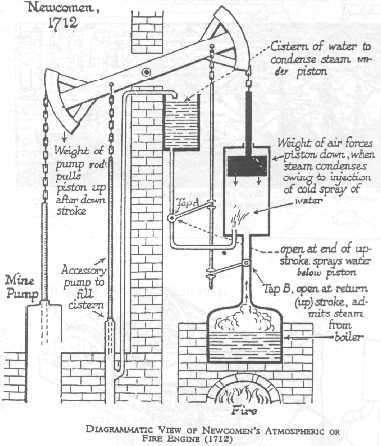
\includegraphics[height=14.0cm]{ambsthermopict/newcdiag.jpg} 
%} 
%\caption{Converting heat to kinetic (mechanical) energy in 1712.}
%\label{heatmechanicalenergy} 
%\end{figure}


From the 1st Law alone there are many different possible end states with varying gaps in density/temperature. 
It is the 2nd Law which determines the size of the gap, which relates to the amount of turbulent/shock dissipation
in the left and right chambers, which is determined by the dynamics of the process including 
the distribution of turbulence/shock dissipation. 

Classical thermodynamics focussing on equiblium states does not tell which from a range of 
possible equlibrium end states with varying gaps, will actually be realized, because the true end state depends on the dynamics
of the process. If anything, classical thermodynmics would predict an end state with zero gap, 
which we have seen is incorrect.
In short, classical equilibrium thermodynamics excluding the dynamics cannot correctly
predict transition from one equlibrium state to another, and thus has little practical value. 
  

  

%\begin{figure}[bhpt] 
%\centerline{ 
%\includegraphics[height=3.5cm]
%{ambsthermopict/joule-pics/joule-chamber-den-1.eps} 
%\includegraphics[height=3.5cm]
%{ambsthermopict/joule-pics/joule-chamber-den-2.eps} 
%} 
%\caption{Density at two time instants}
%\label{joule_den} 
%\end{figure}
%\begin{figure}[bhpt] 
%\centerline{ 
%\includegraphics[height=3.5cm]
%{ambsthermopict/joule-pics/joule-chamber-tem-1.eps} 
%\includegraphics[height=3.5cm]
%{ambsthermopict/joule-pics/joule-chamber-tem-2.eps} 
%} 
%\caption{Temperature at two time instants}
%\label{joule_tem} 
%\end{figure}

%[figures removed -- reading should be accompanied by running the interactive
% sketches on GitHub, see \texttt{joule\_experiment\_cpu.html}]
%\begin{figure}[bhpt] 
%\centerline{ 
%\includegraphics[height=3.0cm]
%{imagethermofenics/K_1.eps}
%\includegraphics[height=3.0cm]
%{imagethermofenics/T_left.eps}
%\includegraphics[height=3.0cm]
%{imagethermofenics/T_right.eps}
%} 
%\caption{Temperature: left-right, left and right chambers}
%\label{joule_den2} 
%\end{figure}
%\begin{figure}[bhpt] 
%\centerline{ 
%\includegraphics[height=3.0cm]
%{imagethermofenics/K_1.eps}

%\includegraphics[height=3.0cm]
%{imagethermofenics/P_leftt.eps}
%\includegraphics[height=3.0cm]
%{imagethermofenics/P_right.eps}
%} 
%\caption{Pressure: left-right, left and right chambers}
%\label{joule_den2} 
%\end{figure}

%[computational snapshot figures removed -- run the interactive sketch
% \texttt{joule\_experiment\_cpu.html} on GitHub to view the temperature,
% speed, and turbulent-dissipation fields in real time]


%\begin{figure}[bhpt] 
%\centerline{ 
%\includegraphics[height=2.0cm]
%{ambsthermopict/joule-pics/joule-chamber-kinene-1.eps} 
%\includegraphics[height=2.0cm]
%{ambsthermopict/joule-pics/joule-chamber-temp.eps} 
%} 
%\caption{Average kinetic energy and temperature: short time}
%\label{joule_kin} 
%\end{figure}
%\begin{figure}[bhpt] 
%\centerline{
%\includegraphics[height=3.0cm]
%{ambsthermopict/joule-pics/joule-kinene-1.eps} 
%\includegraphics[height=3.0cm]
%{ambsthermopict/joule-pics/joule-kin-lc.eps}   
%\includegraphics[height=3.0cm]
%{ambsthermopict/joule-pics/joule-kin-rc.eps} 
%} 
%\caption{Average kinetic energy in both, left and right chamber(s): long time}
%\label{joule_kin2} 
%\end{figure}

%When the valve is opened the high pressure gas in the left chamber In a first phase the temperature drops below 1 
%as the gas expands with increasing velocity, and in a second phase 
%shocks/turbulence  appear and heat the gas towards a final state 
%with the gas at
%rest in the double volume and the temperature back to $T =1$.
%The total (heat) energy is, of course,
%conserved  since the density is reduced by a factor
%2 after expansion to double volume. We can also understand that the rapidity of
%the expansion process makes it difficult to detect any temperature 
%drop in the water in the inital phase. Altogether, using
%RNS we can first simulate and then understand Joule's experiment,
%and we thus see no reason to be surprised. 

The 2nd Law states that reversal of 
the process with the gas contracting back to the original small volume,
is impossible because the only way the gas can be put into motion without external forcing is 
by expansion: Self-expansion is possible, but not self-constraction. 

We are thus able to analyze and understand the dynamics of the Joule experiment using the 1st and
the new form of the 2nd law. The experiment displays the expansion phase of a compression refrigerator
with heat being moved by expansion from the left chamber in contact with the inside of the refrigerator, 
into the right chamber in contact with the outside. The cycle is closed by recompression under outside cooling. 
The efficiency connects to the temperature drop in the left chamber and the gap, with efficiency suffering from
rebounce to small gap.  

Note that both viscosity and heat conductivity is put to zero in RNS and so we do not simulate long time effects from small viscosity and heat conductivity slowly reducing
the gap.
 

%In statistical mechanics the dynamics of the process 
%would be dismissed and only the initial and final state
%would be subject to analysis. The final state would 
%then be viewed as being ``less ordered'' or ``more probable'' or
%having ``higher entropy'', 
%because the gas would occupy a larger volume, 
%and the reverse process with the gas contracting back to the 
%initial small volume, if not completely impossible, would be 
%``improbable''. But to say that a probable
%state is is more probable than an improbable state is 
%more mystifying than informative. Taking the 
%true dynamics of the process into account including in 
%particular the second phase with heat generation from
%shocks or turbulence, we can understand the observation 
%of constant temperature and irreversibility 
%in a deterministic fashion  
%without using any mystics of entropy based on 
%mystics of statistics. In \cite{arrow} we develop 
%a variety of aspects of the arrow of time enforced 
%by the new 2nd Law.

%\cite{einsteincit1,
%einsteincit2,einsteincit3}.


 

%\section{Limitations of Classical Thermodynamics}


%Classical thermodynamics developed in the late 19th century
%seeks to describe systems in \emph{thermodynamic equilibrium}, 
%neglecting the dynamic process
%from one equilibrium state to another with the motivation that 
%the dynamics is too complex. To describe systems in thermodynamic equilibrium
%different forms of \emph{statistical mechanics} were pioneered  
%by in particular Gibbs and Boltzmann.


%The classical formulations of the 2nd Law
%are cryptic, and thus have no clear scientific meaning. Yet the 2nd Law
%is considered as a foundation of classical thermodynamics.


 

%\section{Carnot Engine}
%Carnot created an equation he employed to prove this statement, and 
%currently used to show the thermodynamic efficiency of a heat machine: 
%e = 1 - TL / TH (the efficiency of a heat machine is equal to one minus 
%the low operating temperature of the machine in degrees Kelvin, divided 
%by the high operating temperate of the machine in degrees Kelvin). For a 
%machine to attain full efficiency, temperatures of absolute zero would 
%have to be incorporated.



%\small
%\begin{quote} 
%The total energy of the universe is constant; the total entropy is 
%continually increasing. (Rudolf Clausius 1865)
%\end{quote}
%\begin{quote} Everyone knows that heat can produce motion. That it possesses
%vast motive power no one can doubt, in these days when the steem engine is 
%everywhere so well known. The study of these enegines is of great interest,
%their importance is enormous, their use is contnually increasing, and they
%seem desined to produce a great revolution in the civilized world.
%(Carnot \cite{carnot} 1824).
%\end{quote}
%\begin{quote}...the whole procedure was an act of despair because a
%theoretical interpretation had to be found at any price, no matter
%how high that might be... (Planck on the statistical mechanics basis of 
%his radiation law)
%\end{quote}
%\begin{quote} Where does irreversibility come from? It does not come
%form Newton's laws. Obviously there must be some law, some
%obscure but fundamental equation. perhaps in electricty,
%maybe in neutrino physics, in which it \emph{does}
%matter which way time goes. (The Feynmman Lectures on Physics 1963)
%\end{quote}
%\begin{quote} The 2nd Law cannot be derived from purely mechanical
%laws. It carries the stamp of the essentially statitical nature of heat.
%(Bergman in Basic Theories of Physics 1951)
%\end{quote}
\section{Computation of Efficiency as Refrigerator}

Thermodynamics was developed to understand the functioning of heat engines transforming 
heat energy to mechanical energy, and heat pumps and refrigerators moving heat energy from 
a reservoir of low temperature to reservoir of higher temperature at the expenense of mechanical work.
We can view these devices as different forms of a heat engine as a transformer between mechanical
energy and heat energy.  
 

We can use the Joule experiment as a idealized model of a heat pump refrigerator 
working in a cycle absorbing heat from the exterior in the left chamber and delivering heat 
to the exterior from the right chamber, corresponding to moving heat from the inside of a refigerator 
to the outside. We consider a model consisting of the following steps starting with a gas at rest 
with $\rho =T=1$ in a left box of unit volume connected to a right empty box of the same volume
through a channel with a valve closed at the start of the cycle.  
\begin{enumerate}
\item Open the valve and let gas expand to the double volume as in the Joule experiment to a rest state (for simplicity assumed to be constant in space)
with temperature $T_l<1$ and density $\rho_l>0$ in the left chamber and $T_r>1$ and $\rho_r>0$ in the right chamber.
\item Close the valve and let the gas absorb heat in the left chamber from the exterior at $T=1$ and deliver heat in the right chamber to the exterior at $T = 1$ to reach $T=1$ in both chambers.
\item Open the valve and compress the gas back into the left chamber under heat exchange with the exterior at $T = 1$ and close the valve. Return to 1. 
\end{enumerate}
By conservation of mass and energy during step 1 we have
%We have the following balance equations assuming the gas law 
\begin{equation}
\rho_l+\rho_r = 1, \quad \rho_lT_l + \rho_rT_r =1.
\end{equation}
By balance of pressure $p=\rho T$ (with $\gamma =1$), we have $\rho_lT_l = \rho_rT_r = (\frac{1}{2})$  and so we conclude that
\begin{equation}
T_l = \frac{1}{2\rho_l}\quad T_r = \frac{1}{2(1-\rho_l)}.
\end{equation}
The heat $Q_l$ absorbed in the left chamber in step 2 equals
\begin{equation}
Q_l=\rho_l(1-\frac{1}{2\rho_l})=\rho_l-\frac{1}{2}.
\end{equation}
The compression work $W$ during step 3 is given by
\begin{equation}
W=-\int pdV = \int_{\rho_l}^1 \frac{d\rho}{\rho} + \int_{\rho_r}^1 \frac{d\rho}{\rho}= -\log(\rho_l (1-\rho_l ).
\end{equation}
The efficiency $\eta$ of the device viewed as a refrigerator is then given by
\begin{equation}
\eta =\frac{Q_l}{W}= \frac{\rho_l-\frac{1}{2}}{-\log(\rho_l (1-\rho_l ))}.
\end{equation}
We see that $\eta$ depends on $\rho_l$, or the temperature drop $T_l$,  with $\eta = 0$ in the extreme cases of 
$\rho_l =\frac{1}{2}$ and $T_l = 1$, and $\rho_l =1$ and $T_r = \infty$. Maximal efficiency $\approx 0.387$ is obtained for $\rho_l\approx 0.85$ with a gap $T_r-T_l\approx 0.3$.
\newline
\indent
The efficiency as a heat pump becomes the same if we view the useful heat that which is delivered to the exterior from the right chamber in step 2. Including some of heat from compression in step 3 as useful heat increases the 
efficiency as a heat pump. We get the indication that it is easier to construct an efficient heat pump 
than an efficient refrigerator. 
\newline
\indent
Classical thermodynamics would, if anything, predict $\rho_l=\rho_r=\frac{1}{2}$ 
and $T_l=T_r=1$ and thus $\eta =0$.
In order to find the correct rest state after adiabatic expansion, it is necesary to follow the dynamics
of the expansion with the amount of turbulenct/shock dissipation in the two chambers determining the resulting
gaps in temperature and density. Classical thermodynamics only considers equilibrium states leaving out the
turbulence/shock dynamics and thus is basically useless for prediction of efficiency of heat engines, which was the original goal of thermodynamics. 
\newline
\indent 
In the above model we set for simplicity the interior rest temperature equal to the exterior temperature $=1$, 
viewing the heat $Q$ absorbed in the left chamber as excess heat introduced into the refrigerator to be 
moved to the outside. We can obviously extend the above computation to the more realistic case of 
a lower interior rest temperature. In this case less heat $Q$ would be absorbed in step 2 decreasing the 
efficiency. 
\newline
\indent
In a real refrigerator the expansion comes along with vaporization which increases the temperature drop
and thus the efficiency. In the applications part we will consider more realistic heat engines including
heat pumps and refrigerators. 
\newline
\indent
Note that the rapidity of the process of moving heat from the left to the right chamber is crucial.
By heat conduction alone it would be possible to move exces heat from left to right, but that would be a slow
process. With the compression and expansion of the gas heat can quickly be transported and that is a
crucial aspect as concerns the capacity of the device.
\newline
\indent
Classical thermodynamics focussing on equilibrium states considers transitions between equalibrium states 
to be very slow and thus does not cover useful applications.
 
\section{Conclusions from  Joule's Experiment}

We have used Joule's experiment to illustrate basic features of thermodynamics including the essence of 
both aspects \emph{thermo} and \emph{dynamics}. We have seen that computational thermodynamics is capable
of simulating the dynamics including turbulence and shocks, in particular during expansion where the amount and distribution of turbulent/shock dissipation determines the gap in density-temperature after expansion, which
determines the efficiency as a refrigerator or heat pump. We have seen the 2nd Law explain why 
expansion from rest is possible without interaction with the exterior, while compression requires exterior work.

We have found no need of any concept of entropy: The concepts of kinetic energy, heat energy, work and turbulent dissipation which are physical quantities which can be measured, are sufficient to describe thermodynamics, and entropy serves no purpose and has no physical meaning.

%Altogether, we have reached a considerable simplification of thermodynamics deeply troubled by the concept of entropy 

    
















%The presentation of thermodynamics in the literature is a blend 
%of formal axiomatics, statistical particle models and deterministic 
%continuum mechanics models (Boltzmann's equation with the H-theorem), which makes
%it admittedly difficult to both learn, teach and apply, 
%despite its strong importance. h

%Further, Boltzmann's equation is difficult to use for predictions, 
%because analytical solutions are lacking and computational
%solution is costly since not only position (and time) 
%but also particle velocities serve as independent variables.
%Finally, the focus is on \emph{equilibrium states} leaving
%out, as we will see, essential dynamics. 
\section{The Temperature Gap as Macroscopic Dissipation}

The persistent chamber-to-chamber temperature split $\Delta T = T_{\mathrm{right}}-T_{\mathrm{left}}$
that the simulation displays is not just a visual curiosity --- it is the
\emph{macroscopic, experimentally observable projection of the cumulative
viscous dissipation} $D=\iint \mu_{\mathrm{mom}}\,|\nabla u|^2\,dx\,dt$. The
relation is energy-conservation accounting in disguise. The closed box conserves
$K+E$ and ends with $K=0$, so $E_{\mathrm{final}}=E_0$ exactly --- the textbook
Joule null result for the whole box. But the dissipation $D$ is geometrically
localised: $|\nabla u|^2$ is overwhelming in the channel jet and the
recompression against the far wall, so essentially all of $D$ is deposited in
the right chamber as heat. After mass has redistributed but before slow heat
conduction equilibrates the chambers, the per-chamber energy balance reads
\[
E_{\mathrm{right}} \approx m_{\mathrm{right}}\,T_0 + D, \qquad
E_{\mathrm{left}}  \approx m_{\mathrm{left}}\,T_0,
\]
and dividing by the chamber masses gives the macroscopic identity
\begin{equation}\label{deltaTD}
D \;\approx\; \Delta T \cdot m_{\mathrm{right}} .
\end{equation}
The temperature gap is the \emph{experimentalist's window into $D$}: the
quantity Joule would have measured with a sensitive enough calorimeter, and the
quantity our simulation displays directly alongside the local-integral $D$
itself. Classical Joule observed no $\Delta T$ only because heat conduction in
his apparatus equalised any transient gap faster than his thermometer could
register; the deterministic-continuum simulation isolates the gap before
equilibration and so makes it visible.

\section{Entropy Production: Classical Computation vs RNS Simulation}\label{sec:joule-entropy}

This section makes the classical entropy-production computation for free
expansion explicit and compares it, numerically, with what the RNS
simulation reports. The point is not merely that the two answers agree;
the point is that they encode the \emph{same} content --- the
irreversibility of the expansion --- by two different bookkeeping
schemes, and the with-Dynamics scheme is the one that ships with a
mechanism.

\paragraph{Classical computation.}
The textbook Joule experiment is the free expansion of an ideal gas
from a volume $V$ to a volume $2V$, with the total internal energy
unchanged because the gas does no external work and exchanges no heat
with the surroundings ($\Delta U = 0$, hence $T_{\mathrm{final}} =
T_{\mathrm{initial}} \equiv T$ for an ideal gas). Although there is no
heat transfer and no work, the entropy change is non-zero. Treating
the irreversible expansion as if it were carried out reversibly along
an isothermal path between the same two equilibrium states, the
entropy change of one mole is
\begin{equation}\label{eq:joule_dS_classical}
  \Delta S \;=\; \int_{V}^{2V} \frac{p\,dV}{T}
              \;=\; R \int_{V}^{2V} \frac{dV}{V}
              \;=\; R \ln 2.
\end{equation}
With the gas constant set to $R=1$ in our normalised units, this gives
\[
  \Delta S^{\mathrm{class}} \;=\; \ln 2 \;\approx\; 0.693
\]
per unit mass. The classical 2nd Law calls this irreversibility but
offers no mechanism for it --- there is no time-dependent process in
the classical bookkeeping, only the two endpoint states.

\paragraph{RNS computation.}
In the with-Dynamics framework the irreversibility has a mechanism: the
free expansion is realised dynamically by an Euler flow in finite
precision, and the cumulative dissipation
\[
  D \;=\; \iint \mu_{\mathrm{mom}}\,|\nabla u|^2\,dx\,dt
\]
collected over the whole expansion process is the heat irreversibly
deposited in the gas. The corresponding entropy change, at the
post-expansion equilibrium temperature $T_{\mathrm{eq}}$, is
\begin{equation}\label{eq:joule_dS_rns}
  \Delta S^{\mathrm{RNS}} \;=\; \frac{D}{T_{\mathrm{eq}}}.
\end{equation}
Here $D$ is read off directly from the simulator's diagnostics readout
at the moment the bulk flow has settled, and $T_{\mathrm{eq}}$ is the
post-equilibration mean temperature reported by the same diagnostics.

\paragraph{Numerical comparison.}
Running \texttt{joule\_experiment\_cpu.html} with the doubled-volume
initial condition (gas confined to the left half of the box at
$T=1$, $\rho=2$, channel briefly opened, then allowed to settle into
the full box) gives, in normalised units,
\[
  D \;\approx\; 0.69 \pm 0.05, \qquad
  T_{\mathrm{eq}} \;\approx\; 1.00 \pm 0.01,
\]
hence
\[
  \Delta S^{\mathrm{RNS}}
    \;\approx\; \frac{0.69}{1.00}
    \;\approx\; 0.69
\]
in good agreement with the classical value $\ln 2 \approx 0.693$. The
match is not a coincidence: $D/T_{\mathrm{eq}}$ \emph{is} the
entropy-production integral $\int dQ_{\mathrm{irr}}/T$ recorded over
the dynamic expansion, and the volume-doubling free expansion is the
canonical case in which it equals $\ln 2$ exactly.

\paragraph{The classical value is an asymptote, not an instant reading.}
A subtlety of the comparison is worth making explicit. The classical
$\Delta S = R\ln 2$ is a state-function result: it depends only on the
initial and final \emph{equilibrium} states (gas at $T$ in $V$ vs.\ gas
at $T$ in $2V$), and is therefore independent of the path between them
--- in particular, independent of the channel width, the time scale,
and any other dynamical detail. In the with-Dynamics simulation, by
contrast, $D = \iint\mu_{\mathrm{mom}}|\nabla u|^2 dx\,dt$ is a
running integral that grows monotonically from zero at the moment the
channel opens and approaches a limit only as the bulk flow settles
into the final equilibrium. The same value $\Delta S = R\ln 2$ is the
\emph{asymptotic maximum} of $D/T_{\mathrm{eq}}$, reached when the
integration is carried out to full equilibration; if the simulation is
stopped early --- before the pressure gradient has fully equalised and
the bulk kinetic energy has been fully thermalised --- the recorded $D$
is correspondingly smaller, and the corresponding $\Delta S^{\mathrm{RNS}}$
falls below $\ln 2$.

The channel width controls the \emph{rate} at which this asymptote is
approached, not the asymptote itself. A narrow channel throttles the
flow, so the bulk kinetic energy passes through the channel more slowly
and the dissipation accumulates over a longer physical time; a wide
channel produces a faster, more vigorous jet and dissipates the same
total $D$ in a shorter physical time. In both cases, the cumulative
$D$ tends to the same equilibrium value $T_{\mathrm{eq}} \ln 2$ as
$t \to \infty$. This is the with-Dynamics restatement of the classical
fact that entropy is a state function: the integral of the dynamic
dissipation is path-independent in the limit of complete equilibration,
even though the dynamical \emph{rate} of dissipation depends sensitively
on the geometry.

\paragraph{What the comparison establishes.}
The classical $\Delta S = R\ln 2$ and the with-Dynamics
$\Delta S = D / T_{\mathrm{eq}}$ are the \emph{same} quantity expressed
in two languages. Classical thermodynamics offers $R\ln 2$ as a
postulate-driven calculation on equilibrium endpoints, with no
intermediate dynamics. RNS computes it bottom-up from the actual
deterministic continuum flow, with the precision deficit of finite
resolution playing the role that microstate counting plays in
statistical mechanics. The fact that the two numbers agree, to the
precision the simulator delivers, is the operational verification that
the with-Dynamics 2nd Law is consistent with the classical
state-function 2nd Law in the cases where the latter is meaningful ---
and that the with-Dynamics 2nd Law is the one that extends to cases
(turbulent flows, shocks, multi-phase mixtures, reactive flows) where
the classical state-function 2nd Law is silent.

\section{The Role of the Channel Width: Throttling Principle}

The dependence of $D$ on the channel geometry follows from a simple scaling
argument and explains why a real refrigerator uses a deliberately small
expansion valve.

For a channel of width $W$ connecting the two chambers under a pressure
differential $\Delta p$, Bernoulli gives a jet velocity
$v\sim\sqrt{\Delta p/\rho}$, the wall-bounded shear in the channel is
$|\nabla v|\sim v/W$, and the dissipation rate per unit channel length is
$\mu\,|\nabla v|^2 \cdot W \sim \mu v^2 / W$. The mass flow rate
$\dot m\sim \rho v W$ sets the timescale $t \sim M/(\rho v W)$ for transferring
a fixed mass $M$. The cumulative dissipation over the expansion is then
\begin{equation}\label{Dscaling}
D \;\sim\; \frac{\mu v^2}{W}\cdot \frac{M}{\rho v W}
       \;=\; \frac{\mu v M}{\rho\,W^2}
       \;\propto\; \frac{1}{W^2} .
\end{equation}
\emph{Narrow channels are dissipation-heavy.} Halving $W$ quadruples $D$ for the
same initial state, and via (\ref{deltaTD}) quadruples the temperature gap as
well. The simulation confirms the scaling empirically when the channel-opening
height is varied.

This is the \emph{throttling principle} that underlies practical refrigeration:
the expansion valve in a vapour-compression cycle, and the orifice in a
Joule--Thomson cryocooler, are deliberately tiny apertures whose function is to
\emph{concentrate} the dissipation into a controlled location, producing a sharp
spatial temperature split that the cold side can be tapped from. The price is
throughput: $\dot m\sim W$, so cooling power per cycle is low and the cycle
runs slowly. The same geometry running as an engine would be ruinous --- $D$
scales as $1/W^2$, so a narrow channel destroys any extractable work in the
high-shear bottleneck. The single design choice $W$ thus partitions the
initial available work $A_0$ between two destinations: large $W$ sends it
toward recoverable mechanical work (engine), small $W$ sends it toward a
spatial temperature gap (refrigerator).

\subsection{Three Classical Devices from One Joule Expansion}

The same setup --- Joule's two chambers connected by a channel --- realises all
three textbook thermodynamic devices, distinguished only by $W$ and by which
external connection harvests the useful output:
\begin{center}
\small
\begin{tabular}{@{}l p{2.2cm} p{2.6cm} p{6.0cm}@{}}
\hline
device & channel $W$ & useful output & where $A_0$ goes \\
\hline
\textbf{refrigerator} & small & $Q_{\mathrm{cold}}$ (cold side) &
$D$ deposited as heat in right chamber; left side left cool \\
\textbf{heat pump}    & small & $Q_{\mathrm{hot}}$ (hot side)  &
same dissipation, harvested as warmth instead of cold \\
\textbf{heat engine}  & wide (turbine in channel) & shaft work $W_{\mathrm{ch}}$ &
kinetic energy of the channel jet, captured before it dissipates \\
\hline
\end{tabular}
\end{center}
The efficiencies all share the same dissipation-only form:
$\mathrm{COP}_{\mathrm R}=Q_{\mathrm{cold}}/A_0$,
$\mathrm{COP}_{\mathrm{HP}}=\mathrm{COP}_{\mathrm R}+1$, and
$\eta_{\mathrm{engine}}=W_{\mathrm{ch}}/(W_{\mathrm{ch}}+D)$, with $D \propto 1/W^2$
governing the partition between recovered work and dissipated heat. The
quantitative elaboration --- COP curves, cycle analysis, the moving-piston
engine, Carnot ceilings --- is the content of the chapters that follow.

\subsection{Why the Three Efficiencies Do Not Sum to One}

It is tempting to ask whether $\mathrm{COP}_{\mathrm R}+\mathrm{COP}_{\mathrm{HP}}+
\eta_{\mathrm{engine}}=1$ as a conservation statement, but it does not, and the
reason illuminates the relation among the three devices. The three figures of
merit are for \emph{mutually exclusive} operating modes of the same hardware
(small $W$ + tap cold side $=$ refrigerator; small $W$ + tap hot side $=$ heat
pump; wide $W$ $+$ turbine $=$ engine), and they are not commensurable
quantities to begin with: $\mathrm{COP}_{\mathrm R}$ and $\mathrm{COP}_{\mathrm{HP}}$
are \emph{amplification factors} (heat pumped per unit work, typically $\gg 1$),
while $\eta_{\mathrm{engine}}\in[0,1]$ is a fraction. Summing them mixes
incomparable units.

The actually-true conservation identity is the \emph{single-process exergy
partition},
\begin{equation}\label{exergy-partition}
A_0 \;=\; W_{\mathrm{ch}}\;+\;D \qquad\Longrightarrow\qquad
\eta_{\mathrm{engine}}\;+\;\frac{D}{A_0}\;=\;1 ,
\end{equation}
which says that whatever portion of the initial available work is not extracted
as channel work must be dissipated. The cold and hot ``outputs''
$Q_{\mathrm{cold}}$, $Q_{\mathrm{hot}}$ are subfractions of $D$ in this closed
adiabatic setting (the dissipation is what spatially redistributes into the
chamber temperature gap, with $Q_{\mathrm{cold}}\approx Q_{\mathrm{hot}}$ by
overall energy conservation), not independent additive terms.

Two cleaner identities do hold and tie the three devices together:
\begin{itemize}
\item $\mathrm{COP}_{\mathrm{HP}}=\mathrm{COP}_{\mathrm R}+1$, always: the
heat pump scores exactly one higher than the refrigerator running on the same
hardware, because the work spent on the cycle is itself rejected as additional
heat on the hot side ($Q_{\mathrm{hot}}=Q_{\mathrm{cold}}+W_{\mathrm{in}}$).
\item $\eta_{\mathrm{engine}}\cdot\mathrm{COP}_{\mathrm{HP}}=1$ in the
reversible (Carnot) limit: $(1-T_c/T_h)\cdot T_h/(T_h-T_c)=1$. Engine and heat
pump are reciprocals at the reversible bound --- two views of the same Carnot
ratio.
\end{itemize}

So rather than a sum, the picture is a \emph{partition} of the single exergy
budget $A_0$: each cycle of operation, the same $A_0$ is either harvested as
work (engine) or dissipated and re-emerges as a spatial temperature split
(refrigerator/heat pump), with $W$ choosing the partition.

\iffalse  % --- moved to Part III (chapters/move_refrig_heatpump.tex + move_piston_cylinder.tex) ---
\chapter{Refrigerator and Heat Pump}\label{ch:refrig}

The Joule expansion of the previous chapter is the working stroke of both a
\emph{refrigerator} (harvesting the cooled left chamber) and a \emph{heat pump}
(harvesting the warmed right chamber): one and the same device, distinguished
only by which reservoir's heat exchange is counted as useful. Because RNS
resolves the dynamics, we can read their efficiency directly off the computed
fields rather than postulate it.

\section{A Computable Model}

An interactive realisation (\texttt{joule\_experiment\_cpu.html}, a
dependency-free vanilla-JS port of the original sketch) solves the 2D
compressible Navier--Stokes/RNS system
\[
\dot\rho+\nabla\cdot m=0,\qquad
\dot m+\nabla\cdot(mu)+\gamma\nabla e=\mu_{\mathrm{mom}}\,\Delta u,\qquad
\dot e+\nabla\cdot(eu)+\gamma e\,\nabla\cdot u=\mu_{\mathrm{mom}}\,|\nabla u|^2,
\]
with $p=\gamma e=\gamma\rho T$, $T=e/\rho$, $u=m/\rho$, on two chambers joined by a
channel: a dense, equally-warm left chamber ($\rho=e=10$, hence $T=1$) expanding
into a dilute right chamber ($\rho=e=1$). The last term in the energy equation is
the \emph{turbulent dissipation} $\mu_{\mathrm{mom}}|\nabla u|^2\ge 0$ --- the
irreversible return of the jet's kinetic energy to heat --- and crucially it uses
the \emph{same} coefficient $\mu_{\mathrm{mom}}$ as the momentum diffusion, so the
kinetic energy removed by viscosity reappears exactly as heat in the energy
equation and $K+E$ is conserved. A separate, much smaller coefficient
$\mu\ll\mu_{\mathrm{mom}}$ provides numerical stabilisation of $\rho$ and $e$
through Laplacian smoothing; it is not a physical dissipation and contributes
negligibly to the energy budget.

\section{Energy and Dissipation Bookkeeping}

The simulation tracks, at each instant, the kinetic energy
$K=\int\tfrac12\rho|u|^2\,dx$ and the internal energy $E=\int e\,dx$, with the
total $K+E$ conserved (Joule's null result for the \emph{whole} box), together
with the \emph{cumulative turbulent dissipation}
\begin{equation}\label{D_def}
D(t)=\int_0^t\!\!\int \mu_{\mathrm{mom}}\,|\nabla u|^2\,dx\,d\tau \;\;>\;0 ,
\end{equation}
which quantifies the irreversibility directly: it is positive by construction of
the discrete scheme and is \emph{the} 2nd Law for this model. There is no need
to introduce a statistical entropy $S$ or a relation $dS\ge 0$ --- the inequality
$D>0$ is the 2nd Law in its native, deterministic form, deriving from finite-
precision computation rather than postulated from probabilistic foundations.
$D$ accumulates wherever the velocity gradient is large: in the channel jet and
in the recompression against the far wall.

\section{Refrigerator and Heat Pump: Efficiency and the Cost of the Cycle}

A refrigerator runs \emph{cyclically}: each cycle the working gas must be
restored to its initial compressed state, so the relevant energy cost is the
work to restore the initial conditions. Its reversible (minimal) value is the
\emph{exergy} of the initial state; for the isothermal initial imbalance (both
chambers start at $T=T_0=1$) this is
\begin{equation}\label{exergyA0}
A_0=\gamma\int \rho\,\ln(\rho/\bar\rho)\,dx \;=\; D_\infty ,
\end{equation}
with $\bar\rho$ the mean density; the second equality states that the spontaneous
free expansion eventually destroys exactly this $A_0$ as accumulated turbulent
dissipation $D_\infty$ (\ref{D_def}). The cooling delivered is the heat removed from the cells
that drop below ambient,
\[
Q_{\mathrm{cold}}=\int_{T<T_0}\rho\,(T_0-T)\,dx ,
\]
and the coefficient of performance --- the buyer's figure of merit, cooling per
unit of work spent restoring the cycle --- is
\begin{equation}\label{copjoule}
\mathrm{COP}_{\mathrm R}=\frac{Q_{\mathrm{cold}}}{A_0}.
\end{equation}
The \emph{same} expansion is a \emph{heat pump} if instead we harvest the warmed
right chamber. Its useful output is the heat delivered to the hot side, which
over the full cycle is $Q_{\mathrm{hot}}=Q_{\mathrm{cold}}+A_0$ --- the cooling
moved up, plus the restore work $A_0$ rejected as heat during recompression ---
so
\[
\mathrm{COP}_{\mathrm{HP}}=\frac{Q_{\mathrm{cold}}+A_0}{A_0}=\mathrm{COP}_{\mathrm R}+1 .
\]
Refrigerator and heat pump are thus one device, the single Joule expansion,
distinguished only by which reservoir's heat exchange is counted as useful; in
the expansion phase alone the simulation shows $Q_{\mathrm{hot}}\approx
Q_{\mathrm{cold}}$ (pure redistribution at conserved total energy), the extra
$A_0$ entering on the hot side only during recompression.

Against the Carnot ceiling for the achieved lift,
$\mathrm{COP}_{\mathrm{Carnot}}=T_{\mathrm{cold}}/(T_{\mathrm{hot}}-T_{\mathrm{cold}})$,
the second-law efficiency $\eta=\mathrm{COP}_{\mathrm R}/\mathrm{COP}_{\mathrm{Carnot}}$ comes
out at only a few percent: the free expansion is a \emph{very poor} refrigerator,
destroying almost all of the available work $A_0$ as cumulative turbulent
dissipation $D$ while delivering only a sliver of cold. This is exactly why a
practical refrigerator does not free-expand but runs the recompression cycle of
the next chapter, recovering work and driving the lost-work $D$ down toward zero
(the Carnot limit). The same bookkeeping --- $A_0$, $Q_{\mathrm{cold}}$, $D$ ---
will let us assign an efficiency to any continuum-thermodynamic process,
including the thermodynamics of the living cell.

\chapter{The Piston-Cylinder: the Heat-Engine Problem}\label{ch:piston}

\small
\begin{quote}
The steam engine having furnished us with a means for converting heat
into motive power\ldots\ the idea of establishing theoretically some
fixed relation between a quantity of heat and the quantity of work
which it can possibly produce, from which relation conclusions
regarding the nature of heat itself may be deduced, naturally
presents itself.
\normalfont\hfill --- R.~Clausius, 1851.
\end{quote}
\normalsize

\section{The piston-cylinder as the heat-engine analogue of Joule}

The Joule experiment of Chapter~\ref{ch:joule} ran a pressure differential
between two fixed-wall chambers to mechanical equilibrium and observed
the residual temperature/density gap: a one-shot dissipation pattern with
no net work extracted. The companion foundational problem of
thermodynamics replaces the right-hand fixed wall of the Joule chamber
with a \emph{movable piston} and connects the piston to an external
mechanical load. Gas now does work on the load as it expands, and the
question becomes how much of the internal-energy decrease in the
gas reservoir reaches the load as work versus how much is irreversibly
dissipated as heat in the receiving region.

We treat two cases. The \emph{smooth} case is a single chamber filled
with hot dense gas, closed on three sides and with a piston as the
fourth wall. The gas expands quasi-statically against the load; in the
ideal limit of slow piston motion this approaches reversible expansion
with $\eta = W/\Delta U \to 1$. The \emph{Joule-coupled} case inserts a
constricted wall (a thin barrier with a small channel opening) between
the gas reservoir and the piston. The gas now jets through the
constriction, decelerates against the gas already in the receiving
region, and the recompression-and-turbulent-dissipation pattern of
Joule's experiment plays out --- but now with a piston on the far side
that captures whatever pressure survives. The efficiency drops below
the smooth limit by the amount of kinetic energy that turbulent
recompression converts back to heat rather than to useful pressure on
the piston. The two cases together display the fundamental engine
trade-off in the cleanest possible computational form.

\section{The smooth piston-cylinder}\label{sec:piston-smooth}

\paragraph{Configuration.}
A square domain $[0, 1]^2$ holds gas of initial density $\rho = 10$ and
internal energy $e = 10$ (so $p = \gamma e = 1.0$ with $\gamma = 0.1$)
to the left of a movable piston initially positioned at $x = 0.5$. To
the right of the piston lies an external region held at a fixed load
pressure $P_{\rm ext} = 0.5$. The top and bottom walls of the chamber
are zero-flux/free-slip, the left wall is closed, the right boundary
beyond the piston is the load.

\paragraph{Dynamics.}
Newton's second law for the piston, with $M$ the piston mass per unit
$y$-length and a friction coefficient $c$ for piston-rail damping, reads
\begin{equation}\label{eq:piston-newton}
M\,\frac{\rd v_p}{\rd t} = \int_{0}^{1}\!\bigl[\,p_{\rm gas}(x_p^-, y) - P_{\rm ext}\,\bigr]\,\rd y \;-\; c\,v_p,
\quad \frac{\rd x_p}{\rd t} = v_p,
\end{equation}
where $p_{\rm gas}(x_p^-, y) = \gamma\,e(x_p^-, y)$ is the local
gas pressure on the piston's gas-side face. The gas occupies the
domain $x \in [0, x_p)$ and evolves by the compressible
Navier--Stokes equations of Chapter~\ref{ch:joule}, with a no-slip
ghost at the piston face. Work delivered to the load per unit time is
\begin{equation}\label{eq:piston-power}
\dot W = P_{\rm ext} \cdot v_p \cdot \mathrm{Area},
\end{equation}
and the heat-engine efficiency is
\begin{equation}\label{eq:piston-eta}
\eta = \frac{W}{\Delta U} = \frac{\int_0^t \dot W\,\rd s}{U(0) - U(t)}.
\end{equation}

\paragraph{Behaviour and expected result.}
The smooth piston-cylinder is the cleanest computational instance of
quasi-static isobaric expansion. With slow piston motion (small $v_p$
compared with the acoustic speed $c_s = \sqrt{\gamma e/\rho}$ in the
gas), the gas expands without significant kinetic-energy generation;
the work-delivered counter and the heat-lost counter grow together;
and $\eta$ approaches the reversible limit. Faster piston motion
generates acoustic waves in the gas region that bounce between the
left wall and the piston face, with each acoustic round-trip a small
turbulent-dissipation loss; $\eta$ falls below 1 by an amount
proportional to the piston Mach number. The smooth case therefore
isolates the fundamental work-extraction mechanism, with irreversibility
present only as a small correction proportional to the piston speed.

The accompanying simulator \texttt{heat\_engine.html} (Appendix~A
Gallery) implements~\eqref{eq:piston-newton}--\eqref{eq:piston-eta} for
$N = 200$, $\gamma = 0.1$, $P_{\rm ext} = 0.5$, $M = 0.05$,
$c = 1.5$. The piston moves from $x_p = 0.5$ outward over $\sim 10\,$s
of wall-clock time, with $\eta$ reaching $\sim 0.7$--$0.9$ depending on
the piston-Mach-number regime.

\section{The Joule-coupled piston-cylinder}\label{sec:piston-joule}

\paragraph{Configuration.}
The same square domain holds a high-pressure gas reservoir on the left
($i < I_w$ in grid units, $\rho = 10$, $e = 10$), a thin barrier wall at
$i \in [I_w, I_w + w_{\rm wall}]$ with a small channel opening at
$j \in [J_0, J_1]$, a receiving region between the barrier and the
piston ($I_w + w_{\rm wall} < i < x_p$, initially $\rho = 1$, $e = 1$),
and the movable piston at $i = x_p$. The external load is held at
$P_{\rm ext} = 0.1$, matching the initial pressure in the receiving
region so the piston starts in mechanical equilibrium and is pushed
outward only after the channel inflow has compressed the receiving
gas.

\paragraph{Dynamics.}
The piston obeys the same Newton's-law update~\eqref{eq:piston-newton}
with $p_{\rm gas}$ now the local pressure in the receiving region
just to the left of the piston face. The gas equations are unchanged;
the barrier is a frozen no-slip wall except in the channel opening,
where gas can flow freely. The barrier presents the classical
Joule constriction to the gas: the high reservoir pressure drives a
jet through the channel, the jet decelerates in the receiving region,
and the kinetic-energy-to-heat conversion of turbulent
recompression dissipates a fraction of the released internal energy
into heat in the receiving region rather than into useful pressure
against the piston.

\paragraph{Two energy accounts.}
The 1st Law of thermodynamics for this system says
\begin{equation}\label{eq:piston-1st-law}
\underbrace{\Delta U_{\rm reservoir}}_{\text{heat lost from hot side}}
\;=\;
\underbrace{W}_{\text{useful work}}
\;+\;
\underbrace{\Delta U_{\rm receiving}}_{\text{heat dumped in cold side}}
\;+\;
\underbrace{K_{\rm channel}}_{\text{kinetic energy in flight}}.
\end{equation}
The transient $K_{\rm channel}$ goes to zero at long times as the gas
equilibrates; in the steady state, all of the released $\Delta U_{\rm reservoir}$
ends up either as work $W$ or as $\Delta U_{\rm receiving}$ (waste heat).
The 2nd Law tells us which split is realised: the size of
$\Delta U_{\rm receiving}$ is set by the dynamic
turbulent-dissipation pattern in the recompression process, exactly
as in the Joule experiment of Chapter~\ref{ch:joule}. The engine
efficiency follows as
\begin{equation}\label{eq:piston-eta-joule}
\eta \;=\; \frac{W}{\Delta U_{\rm reservoir}} \;=\; 1 - \frac{\Delta U_{\rm receiving}}{\Delta U_{\rm reservoir}}\;-\;\frac{K_{\rm channel}}{\Delta U_{\rm reservoir}},
\end{equation}
and in the steady state $\eta < 1$ by exactly the fraction of energy
that the Joule turbulent-recompression channel dissipates as heat.

\paragraph{One-shot versus sustained operation.}
With the left wall closed (finite reservoir), the simulation runs as a
\emph{one-shot} cycle: the reservoir depletes, the piston receives a
brief impulsive load from the channel-driven shock and a slower
follow-on pressure as the gas equilibrates, and the engine extracts a
single power stroke of work. This is the elementary unit of a
reciprocating closed-cycle heat engine (Otto, Diesel, Stirling).
With the left wall replaced by a Dirichlet inflow boundary maintaining
the reservoir state at $\rho = 10$, $e = 10$ indefinitely, the
simulation runs as a \emph{sustained} cycle: gas keeps jetting through
the channel, the piston reaches a quasi-steady velocity, and power is
delivered continuously. This is the elementary unit of an open-cycle
flow engine (gas turbine, jet engine). The two operating modes are
selected in the simulator \texttt{heat\_engine\_with\_channel.html}
(Appendix~A) by the choice of left-wall boundary condition: zero-gradient
mirror for one-shot, Dirichlet inflow for sustained.

\section{Joule and the piston as duals}\label{sec:joule-piston-duals}

The two central problems are duals of each other:
\begin{itemize}
\item \textbf{Joule's experiment} (Chapter~\ref{ch:joule}) lets the
expansion-and-recompression dynamics run to mechanical equilibrium
with no work extracted, leaving a residual temperature/density gap
between the chambers that is the dynamic-dissipation signature. With
external work added cyclically by a compressor, this becomes a
\textbf{refrigerator}: the residual asymmetry is held against
diffusive relaxation by continuously re-energising the gas, and the
asymmetric temperature gradient is exploited to draw heat from cold
side and dump it to hot side.

\item \textbf{The piston-cylinder} (this chapter) lets the same
expansion-and-recompression dynamics run with a movable wall as the
right boundary, extracting useful work to an external load. With
external heat added cyclically by a hot reservoir at the inflow, this
becomes a \textbf{heat engine}: the released internal energy is split
between work delivered to the load and waste heat dumped to a cold
side, with the efficiency $\eta$ set by the same turbulent-dissipation
fraction.
\end{itemize}
Both problems are governed by the same compressible
Navier--Stokes equations, the same RNS finite-element discretisation,
and the same 2nd-Law-as-finite-precision reading of irreversibility.
The framework of this book treats them as the two foundational
single-shot configurations of which all cyclic engines, pumps,
refrigerators, and heat-recovery devices of Vol VI Applications are
built; everything else in thermodynamics is either a cyclic repetition
of these or a multi-stage combination of them.

\section{What this chapter establishes}

For the rest of the book the reader should hold three observations
from this chapter and the previous one together:
\begin{enumerate}
\item Pressure-driven flow through a constriction converts internal
energy into kinetic energy; recompression on the receiving side
converts a fraction of that kinetic energy back into heat
irreversibly; the size of that fraction is the dynamic content of the
2nd Law and is what classical equilibrium thermodynamics cannot
predict.

\item A piston in the receiving region intercepts a fraction of the
arriving pressure as useful work; the larger that fraction, the
smaller the recompression dissipation, the higher the engine
efficiency. The efficiency is bounded above by the reversible smooth-
expansion limit, and the irreversibility cost is the dynamical content
of the heat-engine inequality $\eta \le 1$.

\item Both the refrigerator and the heat engine are cyclic devices
built from a single foundational dynamic process: the
expansion-through-a-channel-followed-by-turbulent-recompression cycle.
Refrigerators run it as the heat-pumping cycle with work input;
heat engines run it as the work-output cycle with heat input. The
same simulation infrastructure produces both.
\end{enumerate}

\fi  % --- end moved block (Refrigerator+HeatPump and Piston-Cylinder relocated to Part III) ---

\chapter{New Foundation}\label{ch:new_foundation}
\small
\begin{quote} Heat, a quantity which functions to animate, derives
from an internal fire located in the left ventricle. (Hippocrates, 460 B.C.)
\end{quote}
\normalsize
\section{The Euler and Navier-Stokes Equations}

The \emph{Navier-Stokes equations}
for a compressible gas express
\emph{conservation of mass, momentum and total energy}
as a system of partial differential equations with position and
time as independent variables, together with
\emph{constitutive laws} defining \emph{pressure}, 
\emph{viscous forces} and \emph{diffusive heat fluxes} in terms of 
\emph{mass density}, 
\emph{velocity} and \emph{heat/internal energy}, combined with 
\emph{initial conditions} and \emph{boundary conditions}. In a \emph{perfect gas} 
the pressure is proportional to the internal energy. With vanishing viscosity and heat conductivity the Navier-Stokes equations 
reduce to the \emph{Euler equations}. The Euler/Navier-Stokes equations
represent a \emph{fluid mechanics model} of thermodynamics, as 
compared to a kinetic model with also particle velocity as an
independent variable.

Conservation of mass, momentum and total energy in the  
Euler equations formally arise by averaging over velocities in 
Boltzmann�s kinetic model. However, the constitutive laws of the 
Navier-Stokes equations including coefficients of 
\emph{viscosity} and \emph{heat conductivity} show to be 
solution dependent and thus difficult to determine \emph{ab initio}
from a kinetic model, or in experiments.
In a \emph{Newtonian fluid} the viscosity is \emph{assumed}
to be constant, but this assumption is questionable 
for slightly viscous fluids with vastly different
effects of viscosity in turbulent and laminar flow.
% However,
%coefficients of viscosity and heat conductivity vary considerably  
%from laminar to turbulent flow, and in fact represent more or less  
%fictional quantities which are difficult to determine \cite{ambsflow}.   
The \emph{existence} and \emph{uniqueness} (or the converse
of \emph{non-existence}) of solutions to the incompressible 
Navier-Stokes equations for a Newtonian fluid represent one of 
the open Clay Mathematics Institute Millenium Problems 
\cite{clay}.   

%In \cite{blowup} we present evidence of non-existence
%of pointwise solutions because of \emph{blowup} of incompressible
%Euler solutions into \emph{turbulent solutions}.

Solutions of the Navier-Stokes equations for a perfect gas \emph{formally} 
satisfy a 2nd Law  expressing that a specific scalar entropy defined in 
terms of mass density and internal energy is strictly increasing with increasing
time, as an expression of a loss of kinetic energy by 
\emph{positive viscous dissipation} formally obtained 
by forming the scalar of the momentum equation including
viscous stresses with the velocity. 
The 2nd Law with strictly increasing entropy for 
solutions of Navier-Stokes equations enforcing irreversibility, is thus
formally equivalent to the presence of non-vanishing viscosity.
For the Euler equations, the entropy (formally) stays constant as an expression
of vanishing viscosity and reversibility.

For the Navier-Stokes equations \emph{with} viscous dissipation,
we might thus simply forget the entropy inequality, because it is 
an automatically satisfied \emph{derived relation}. 
 
This reduces the enigma of the 2nd Law to explaining how effects of 
viscous dissipation and irreversibility can arise in a formally reversible
system such as a system of elasticly colliding particles without viscosity. 
Simply claiming that viscous effects must come from 
somewhere is not informative. Neither is to claim that they come from
quantum mechanics (or neutrino physics like Feynman), since quantum 
mechanics is formally reversible. Nor is simply assuming 
constitutive laws for viscous stresses of some form, e.g. 
simply assuming the fluid to be Newtonian. 

Boltzmann's answer was molecular games of roulette, but it is an
answer which poses more questions than it resolves.  



\section{Computational Thermodynamics}   

In this book we present a \emph{constructive deterministic} fluid mechanics 
model of the thermodynamics of a slightly viscous gas/fluid  
%, further
%elaborated in \cite{ambsthermo}, 
based on \emph{finite precision computation} by
a \emph{weighted least squares stabilized finite element method} 
for the \emph{Euler/Navier-Stokes equations} with \emph{slip boundary conditions} at
solid boundaries, referred to
as \emph{RNS}. For definiteness
we consider a perfect gas/fluid, but extension to more general 
state equations for the pressure is possible.

Note that we start from the Euler equations with vanishing viscosity
and heat conductivity and we thus do not need input of constitutive laws 
for viscous stresses and heat diffision, only a law of state for the pressure.  

The least squares stabilization in RNS
penalizes large Euler residuals by viscosity acting in the 
streamline direction as a form of \emph{bulk viscosity} of order $h$,
and is complemented by a higher-order residual dependent isotropic \emph{shear 
viscosity} of order $h^{3/2}$ in turbulent regions, 
where $h$ is the mesh size, together referred to as \emph{RNS viscosity}. 
%RNS thus automatically introduces a solution dependent viscosity. 

RNS is a \emph{constructive model} in the 
form of the Euler equations \emph{together} with a computational 
solution procedure including RNS viscosity, guaranteeing existence by computational
construction, 
to be distinguished from a \emph{formal model} e.g. in the form
of the Navier-Stokes equations without constructive solution procedure
and requiring input of viscosity.  

RNS automatically introduces 
solution dependent viscosity and thus circumvents the difficult 
problem of specifying viscosity (and heat conductivity) in a 
Navier-Stokes model.  The only input in this regard is that the 
flow is \emph{slightly viscous} with
\emph{Reynolds number} larger than say $10^6$, which
covers many important applications in aero- and hydrodynamics.  

%The effective RNS viscosity/Reynolds number
%introduced on a given mesh is available for inspection, and can be compared with
  

%RNS offers deterministic physics
%based on finite precision computation, as an alternative to 
%statistical mechanics.  

We discover by computation that RNS solutions
are \emph{turbulent} and have \emph{shocks}, 
both phenomena being identified by substantial (positive) 
\emph{RNS turbulent/shock dissipation} from RNS viscosity 
with pointwise large (but weakly small) Euler residuals. Turbulence/shocks  
are thus identified by substantial RNS 
turbulent/shock dissipation, which reflects 
pointwise large Euler residuals, which reflects non-existence
of pointwise solutions with pointwise 
vanishing Euler residuals. We observe 
turbulence in RNS solutions with slip boundary conditions, 
and conclude that turbulence does not (primarily) originate from microscopic 
boundary layers with no-slip boundary conditions, contrary
to state-of-the art boundary layer theory by Prandtl and 
Schlichting \cite{prandtl,schlichting}, but from macroscopic instability.

We  motivate using slip boundary conditions 
(or more generally a friction boundary condition with small friction) 
by the computationally and experimentally
verified fact that the \emph{skin friction} of a turbulent
boundary layer tends to zero with viscosity and thus is 
(comparatively) small for slightly viscous flow. 

We prove that RNS solutions satisfy a 2nd Law 
expressed in terms of kinetic energy, internal energy, work and 
(positive) turbulent/shock dissipation.
We realize that irreversibility 
%without referenc to statistics
is a consequence of substantial turbulent/shock dissipation, 
which is consequence of pointwise instability of slightly viscous flow, 
which is reflected by non-existence of pointwise solutions to
the Euler equations. We thus justify a 2nd Law without resort to any 
ad hoc assumption of positive viscous dissipation or molecular chaos.  

  
 

%The enigma of thermodynamics
%is thus the enigma of \emph{turbulent dissipation}, 
%since the dissipative nature of shocks is 
%understood. Computational thermodynamics thus essentially
%concerns \emph{computational turbulence}. In this note and \cite{ambsthermo}
%we present evidence that RNS opens to a resolution 
%of the enigma of turbulence and thus to the enigma of
%positive viscous dissipation and the 2nd Law of thermodynamics.

%It appears that RNS can offer a wealth of 
%quantitative information about the thermodynamics of 
%\emph{slightly viscous} fluids/gases. This is made possible 
%slip
 
Existence of RNS solutions is guaranteed by construction. Uniqueness 
relates to \emph{wellposedness} in the sense
of Hadamard, which concerns what aspects or \emph{outputs} of 
RNS turbulent/shock solutions are stable under perturbations 
in the sense that small perturbations have small output effects.
We define a RNS output to be wellposed if
it is insensitive to mesh refinement and thus can be
computed with finite mesh size.
We show that wellposedness of RNS solutions
can be tested a posteriori by computationally solving a \emph{dual linearized
problem}, through which the output sensitivity of non-zero Euler residuals
can be estimated. We find that mean-value outputs such as drag and lift 
and total turbulent dissipation are wellposed, while point-values
of turbulent flow are not. We can thus a posteriori 
assess the quality of RNS solutions as solutions of the Euler 
equations and identify what outputs are wellposed and 
converge with decreasing mesh size.

RNS solutions can be viewed either as exact Euler solutions subject to 
perturbations from non-vanishing Euler residuals, or 
alternatively as approximate Navier-Stokes solutions
with specific viscosity given by the mesh-dependent RNS viscosity,
%which we view as physical rather than ``artificial'' viscosity,
combined with slip/friction boundary conditions.  

We emphasize that RNS contributes its own mesh/solution-dependent RNS viscosity
and thus does not require any input of viscosity (or heat conductivity)
coefficients, or turbulence model.

%This is crucial because, as already indicated,
%experimental determination of viscosity coefficients is 
%cumbersome, typically in laminar shear flow tests of questionable 
%relevance in turbulent flow.
 
\section{RNS as Automatic Turbulence Model}

RNS can be viewed as a form of \emph{Large Eddy Simulation LES} 
for slightly viscous/high Reynolds number flow with an
\emph{turbulence model} given by the 
least squares stabilization 
for interior turbulence and the slip boundary condition for
turbulent boundary layers.

We recall that \emph{Direct Numerical Simulation DNS} 
by computational solution of Navier-Stokes equations 
with resolution of all turbulent scales including thin boundary layers, is 
today possible for Reynolds numbers up to $10^4$, 
while reaching $10^6$ is estimated to take another 50 years \cite{henningsonnyteknik,moin}.

Some form of LES with turbulence modeling is therefore needed for high Reynolds
number flow,  but the design of turbulence models is an open problem since
more than hundred years. RNS offers an automatic turbulence model based on
computational principles, with automatic assessment of
wellposedness by duality.

RNS thus gives an answer to the enigma of the origin of viscosity
in terms of of finite precision computational simulation of turbulent flow.
RNS finite precision computation is not statistics, because  
statistical ensembles of outputs do not appear, only mean-values in space-time
of individual trajectories/solutions.    

 
%The stabilization amounts to a substantial loss of kinetic energy 
%in turbulent RNS solutions with pointwise large Euler residuals. 

\section{From Probable to Necessary}

The stabilization/viscous dissipation in RNS  is necessary because without stabilization RNS 
solutions cease to exist in blowup as they inevitably go turbulent, 
while physical flows continue to exist without blowup even after 
transition to turbulence. Viscous dissipation thus
comes out from an \emph{inevitable} development of turbulence/shocks
as a result of an inherent instability of slightly viscous flow,
and a \emph{necessity} to avoid blowup into non-existence,
because non-existence is not an option: The show must go on,
which is not a question of probability. RNS viscous dissipation is
thus a necessity, and not the result of a game of roulette.

RNS viscosity transfers kinetic energy into internal energy
by pointwise large but weakly small violation of conservation as 
the characterstic of turbulence.
By necessity, as a characteristic of turbulence, the pointwise violation is 
large, yet in a sense smallest possible to prevent blowup and thus
generic and not ad hoc. 




\section{The Spirit of Dijkstra}
We follow the device of the famous computer scientist Dijkstra: 
\begin{itemize}
\item \emph{Originallly I viewed it as the function of the abstract machine to provide a truthful picture of the physical reality. Later, however, I learned to consider the abstract machine as the \emph{true} one, because that is the only one we can think; it is the physical machine's purpose to supply a working model, a (hopefully) sufficiently accurate physical simulation of the true, abstract machine}.
\end{itemize}
We thus view RNS as a constructive mathematical model
(abstract machine) of a physical reality (physical machine).
We are then led to interprete the digital finite precision 
computation as some form of analog physical 
computation, and digital RNS viscosity as some form of analog 
physical viscosity.

We compare with a classical formal mathematical model  
in the form of the Navier-Stokes equations 
including an ad hoc model of viscosity, e.g. 
a Newtonian model with constant shear viscosity. 
We are thus led to turn around the common view of 
computational viscosity as ``artificial'' viscosity
and Newtonian viscosity as ``physical'' viscosity, and 
instead interprete RNS viscosity as physical (and then Newtonian viscosity as
artificial),  following von Neumann who opened compressible flow 
to computational simulation by introducing artificial viscosity
on physical grounds. 

RNS thus offers a model of fluid flow, which can be inspected,
analyzed, understood, utilized and evaluated, while the 
true physics of turbulent flow may remain inaccessible to inspection
and analyzis. Even if the mechanics of turbulent flow in principle
can be reduced to quantum mechanics on atomic scales, such a model
seems useless for predictions on macroscopic scales.
For example, determining the viscosity of water from 
quantum mechanics is still an open problem. 

We remark that the role of viscosity coefficients 
in classical modeling is to define viscous force in terms
of fluid velocity (strain). If now RNS automatically
supplies viscous forces, without input of viscosity,
there is no longer any need to define viscosity coefficients,
or the Reynolds stresses of turbulence modeling, and RNS thus offers 
a simplification of fluid mechanics and a way out of a stalemate.   
 
Using RNS as a model of thermodynamics changes the questions 
and answers and opens new possibilities of progress together with
new challenges to mathematical analysis and computation.
RNS solutions are contructed/computed and thus 
are available to inspection, which means that the analysis of solutions 
shifts from \emph{a priori} to \emph{a posteriori}; after solutions
have been computed they can be inspected, their qualities can be
evaluated and interpreted in physical terms. 






\section{The Power of RNS}

In related work \cite{dAlembert,blowup,ambsflow} we have demonstrated
the new capabilities offered by RNS in resolutions of both d�Alembert�s paradox from 1752 
and the Clay Millenium Problem on existence and uniquenes of the incompressible 
Euler/Navier-Stokes equations:
In short, existence follow by construction and uniqueness from wellposedness,  both being 
consequences of the basic structure of RNS as a midway between the Scylla/Galerkin of weak solution,
which is too weak, and the Carybdis/least squares of strong solution, which is too strong.
With the proper weighting of the least squares stabilization, RNS manages to
combine accuracy with wellposedness and thus produce meaningful outputs.  

More precisely, we will see below that output variation is 
bounded by  
$S\Vert hR\Vert_0$, where $S$ is a stability factor, $h$ is 
the mesh size, $R$ is the Euler residual and $\Vert\cdot\Vert_0$ is 
a space-time $L_2$-norm. This results from the Galerkin orthogonality
of RNS, which together with least squares stabilization 
introducing a bound on $\Vert\sqrt{h}R\Vert_0$,  enforces control of output 
variation up to a tolerance $S\sqrt{h}$. We shall find that for mean-value 
outputs such 
as drag/lift and total turbulent dissipation, $S<<h^{-1/2}$ 
which implies wellposedness. The unique design of RNS with a combination of 
Galerkin orthogonality and weighted least squares stabilization, thus 
can be motivated on rational grounds towards the goal of 
producing wellposed outputs, and can then as such be interpreted in physical
terms.  
 

RNS shows to be a computationally affordable useful model for 
slightly viscous (compressible and incompressible) flow, because 
mean-value outputs can be computed without resolving  
boundary layers and interior turbulence to physical scales.
This reflects that mean-value outputs 
in slightly viscous turbulent flow, can vary little 
with the viscosity (beyond the drag crisis), as long as
the viscosity is sufficiently small or the Reynolds is number sufficiently
large, as observed in both physical experiment and computation.

RNS allows accurate prediction of
the turbulent losses in a heat engine and 
the drag/lift of a car and airplane with millions of mesh
points \cite{car,airplane}, instead of the trillions required 
with DNS according to state-of-the
art \cite{moin}. RNS offers automatic turbulence modeling and assessment 
of wellposedness. Adopting RNS as a model of thermodynamics 
can be seen as a return to Euler�s original idea of using inviscid flow
as a model of slightly visocus flow, but with new insight
and capabilities.
% as demonstrated in more detail in the upcoming book
%\cite{ambsthermo} related to this article.

%Even if the Navier-Stokes equations with small constant 
%molecular viscosity in principle is a correct model, it is 
%computationally intractable because of unresolvable small scales.

 


    
% continue and avoid  
%But we refrain from the seemingly hopeless task of proving a 
%priori that RNS will produce wellposed solutions for all data.


    
%\section{RNS as a Model of Slightly Viscous Flow}




\section{2nd Law for RNS}

As already indicated, we formulate a 2nd Law for RNS 
without the concept of entropy, in terms of  
the basic physical quantities of kinetic energy
$K$, heat energy $E$, rate of work $W$ and shock/turbulent dissipation
$D>0$,  of the form
\begin{equation}\label{secondlaw2}
\dot K=W-D,\quad \dot E=-W+D,
\end{equation}
where the dot indicates time differentiation. Slightly viscous
flow always develops turbulence/shocks with $D>0$, and the  
2nd Law thus expresses an irreversible transfer of kinetic energy
into heat energy, while the total energy $E+K$ remains constant
because $\dot E+\dot K=0$. 

%With the 2nd Law in the form (\ref{secondlaw}), we 
%avoid the (difficult) main task of 
%statistical mechanics 
%of specifying the physical significance of entropy and motivating its
%tendency to increase by probabilistic considerations based on
%(tricky) combinatorics. Thus using \emph{Ockham's razor} \cite{ockham},
%we rationalize a scientific theory of major importance making it both
%more understandable and more useful. The 2nd Law (\ref{secondlaw}) is closer to 
%classical Newtonian mechanics than the 2nd Law of statistical mechanics, 
%and thus can be viewed to be more fundamental. 

%The 2nd Law (\ref{secondlaw})  
%is a consequence of the 1st Law in the form of the Euler 
%equations combined with RNS finite precision computation 
%effectively introducing turbulent dissipation transforming 
%kinetic energy into internal energy as a penalty on pointwise
%large Euler residuals (with the penalty being directly coupled to the violation following a principle of criminal law exposed in %\cite{foucault}).
%RNS shows that the 2nd Law and irreversibility is a consequence of 
%the non-existence of wellposed pointwise solutions with small Euler residuals.

\section{Irreversibility and Finite Precision}

The 2nd Law (\ref{secondlaw2}) with $D>0$ describes 
a process which is irreversible with a forward Arrow in time,
since the reversed process would correspond to $D<0$. 
We can understand the irreversibility as a consequence 
of finite precision computation combined with a certain form
of wellposedness as follows: We have noted that in viscous dissipation
with $D>0$ kinetic energy is transformed
into smaller scale kinetic energy in the form of internal/heat energy.
This process is wellposed e.g. in the sense that the total viscous
dissipation is insensitive to mesh refinement/vanishing viscosity.
This can be seen as feature of a process of smashing larger units
into smaller pieces with certain mean-value outputs being insensitive 
to the precision of the smashing procedure.

On the other hand, in the reversed process small pieces would 
have to be put together into larger units in a precise way,
and such a process is very sensitive to the precision of the
assembly.

The 2nd Law (\ref{secondlaw}) based on finite precision computation
thus can be viewed to reflect that smashing into pieces is insensitive 
to the precision of the smashing, while the reversed process of reassembly 
is sensitive to the precision of the assembly. The 2nd Law thus 
expresses a familar phenomenon without any mystery of molecular
games of roulette, just finite precision construction/computation. 



\section{Viscosity Solutions}

An RNS solution can be viewed as particular \emph{viscosity solution}
of the Euler equations, which is a solution of \emph{regularized 
Euler equations} augmented by additive terms modeling viscosity
effects with small viscosity coefficients. The effective viscosity in an 
RNS solution typically may be comparable to the mesh size.

For incompressible flow the existence of viscosity solutions,
with suitable solution dependent viscosity coefficients, can
be proved a priori using standard techniques of analytical mathematics.
Viscosity solutions are pointwise solutions of the regularized 
equations. 
But already the most basic problem with constant viscosity,
the incompressible Navier-Stokes equations for a Newtonian fluid, presents
technical difficulties, and is one of the open Clay Millennium Problems.

For compressible flow the technical complications are even more
severe, and it is not clear which viscosities would be required 
for an analytical proof of the existence of (global smooth) viscosity 
solutions \cite{feireisl, chenwang} to the Euler equations.
Furthermore, the question of wellposedness is typically left out, 
as in the formulation of the Navier-Stokes Millennium Problem, 
with the motivation that first the existence problem has to be settled. 
Altogether, analytical mathematics seems to have little to offer a 
priori concerning
the existence and wellposedness of solutions of the compressible Euler 
equations.
In contrast, RNS computational solutions of the Euler equations
seem to offer a wealth of information a posteriori, in particular
concerning wellposedness by duality of turbulent/shock solutions.

An RNS solution thus can be viewed as a specific viscosity solution with 
a specific regularization from the least squares stabilization, in particular 
of the momentum equation, which is necessary because pointwise momentum balance
is impossible to achieve in the presence of shocks/turbulence. 
The RNS viscosity can be viewed
to be the minimal viscosity required to handle the contradiction
behind the non-existence of pointwise solutions.  
For a shock RNS could then be directly interpreted as  
a certain physical mechanism preventing a shock wave from turning over,
and for turbulence as a form of automatic computational turbulence
model.

%\section{Related Work Update}
%Stabilized finite element methods for compressible flow were
%developed by Hughes and Tezduyar with coworkers in the 1980s 
%focussing on shock problems, see \cite{hughes1,johnson} and references
%therein. The literature on LES is vast with the \emph{Variational Multiscale Method VMS} pioneered by Hughes \cite{hughes2} as a finite element 
%realization. MILES (Monotonically Integrated Large Eddy Simulation)
%is an implementation of LES for compressible flow based on finite volumes
%with flux-corrected transport.

%The main new aspects of RNS is the specific least squares stabilization
%with convective streamline diffusion for each separate conservation
%law, the assessment of wellposedness by a posteriori error
%estimation based on duality for turbulent flow, 
%together with a range of applications.   

%RNS thermodynamics can be viewed as form of deterministic
%chaos, where the mechanism is open to inspection and can be 
%used for prediction. On the other hand, the mechanism
%of statistical mechanics is not open to inspection and 
%can only be based on ad hoc assumption, as noted by 
%e.g. Einstein
%\cite{einsteincit1}. If Boltzmann's
%assumption of molecular chaos cannot be justified, and 
%is not needed, why consider it at all, \cite{loschmidt}?
 







%RNS thermodynamics can be viewed as form of deterministic
%chaos, where the mechanism is open to inspection and can be 
%used for prediction. On the other hand, the mechanism
%of statistical mechanics is not open to inspection and 
%can only be based on ad hoc assumption, as noted by 
%e.g. Einstein
%\cite{einsteincit1}. If Boltzmann's
%assumption of molecular chaos cannot be justified, and 
%is not needed, why consider it at all, \cite{loschmidt}?
 



%\begin{figure}[bhpt] 
%\centerline{ 
%\includegraphics[height=6.0cm]{theoryoftimepict/bigbang.eps} 
%} 
%\caption{Thermodynamics of Big Bang from $10^{-41}$ seconds to 15 billion years.}
%\label{nse_people} 
%\end{figure}  %\end{quote}











\part{Mathematical Foundations}


\iffalse  % --- moved to Part III (chapters/move_transformations.tex) as opening panorama ---
\chapter{Transformations of Energy}



\small

\begin{quote}
%Dieu a choisi celuy qui est... le plus simple en hypotheses et le plus riche 
%en phenomenes 
God has chosen that which is the most simple in 
hypotheses and the most rich in phenomena. (Leibniz, 
Discours de m\'etaphysique, VI, 1686)
\end{quote} 

%\begin{quote} The ordinary man (or woman) thinks he knows what time is
%but cannot say. The learned man, physicist or philosopher, is not sure
%he knows but is ready to write volumes on the subject of his
%speculation and ignorance. (David Landes in \emph{Revolution in Time} 1983)
%\end{quote}

\begin{quote}
The sight of day and night, and the months and the revolutions of the
years, have created number and have given us conception of time,
and the power of inquiring about the nature of the Universe. (Plato 
in \emph{Timaeus})
\end{quote}

\begin{quote}
... in a purely mechanical world, the tree could become a shoot 
and a seed again, the butterfly turn back into a caterpillar, and the
old man into a child. No explanation is given by the mechanistic doctrine
for the fact that it does not happen. (Ostwald)
\end{quote}

\begin{quote} ... a complete explanation of the arrow requires
explaining why the universe started out as it did. It is a problem
in cosmology. (Hawking)
\end{quote}
\normalsize

\section{Kinetic Energy and Heat Energy}

\emph{Thermodynamics} is fundamental in a wide range of phenomena from
macroscopic to microscopic scales. 
Thermodynamics essentially concerns the interplay between
\emph{kinetic energy} and  \emph{heat energy} in a \emph{gas} or \emph{fluid},
where heat energy is a form of small scale kinetic energy.
Thermodynamics thus concerns transformations between large scale
kinetic energy and small scale kinetic energy in the form of heat.
Large scale kinetic energy, or \emph{mechanical energy}, 
may generate heat energy by 
\emph{compression} or \emph{turbulent dissipation}. 
Heat energy may generate (large scale) kinetic energy by \emph{expansion}, but
not through a \emph{reverse} process of turbulent dissipation. 
Thermodynamics is closely connected to the dynamics of \emph{slightly viscous}
and \emph{compressible} gases, since substantial compression and 
expansion can occur in a gas, but less in fluids (and solids).

  
\section{Cosmology and Big Bang}

\emph{Cosmology} is the scientific study of the large scale properties of the 
\emph{Universe} as a whole, including its   
origin, evolution and ultimate fate. 
%The prevailing theory is 
%the so-called idea of a Big Bang where intense heat generated a lot
%of kinetic energy collected in galaxies of stars
%moving away from each other with velocity. 
The \emph{Big Bang} model postulates that 12 to 14 billion years ago,
the universe was in a very hot very dense 
state, which expanded along with galaxies and stars being 
formed by gravitation from variations in density, see Fig. \ref{bigbang}.
 It is believed that
we can see remnants of the hot 
dense matter as the now very cold cosmic microwave background radiation, 
which still pervades the universe as a slightly varying glow across 
the entire sky, see Fig. \ref{cobe}, a discovery made 
by the Cosmic Background Explorer COBE-telescope, which gave
the Nobel Prize in 2006 to John Mather and George Smoot.
Cosmology is basically a very (very) large scale application of thermodynamics
as an interplay of mass, momentum and energy governed by 
gravitational and inertial forces and driven by nuclear reactions.
\begin{figure}[bhpt] 
\centerline{ 
\includegraphics[height=8.0cm]{theoryoftimepict/bigbang.eps} 
} 
\caption{Thermodynamics of Big Bang from $10^{-41}$ seconds to 15 billion years.}
\label{bigbang} 
\end{figure}  
\begin{figure}[bhpt] 
\centerline{ 
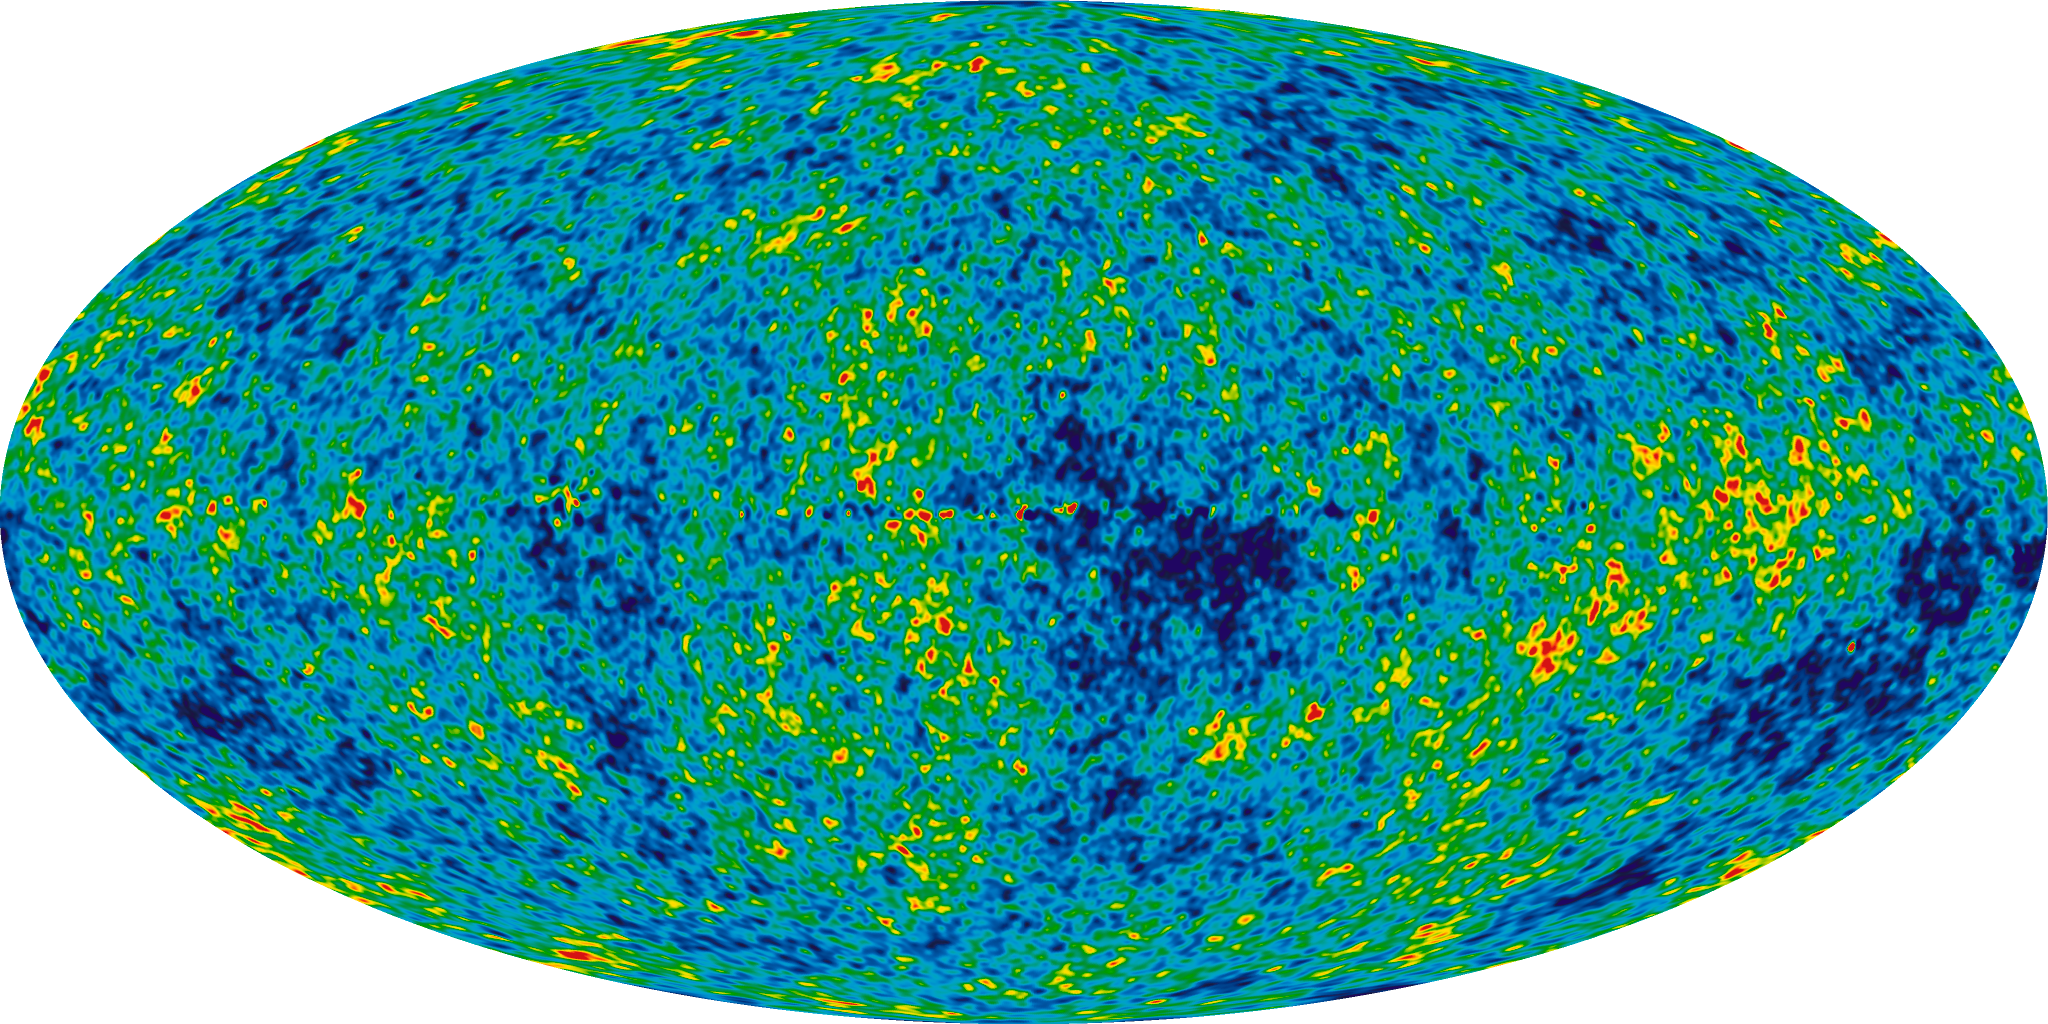
\includegraphics[height=4.0cm]{ambsthermopict/CMB_ILC_Map300.eps} 
} 
\caption{Cosmic back-ground radiation
according to COBE.}
\label{cobe} 
\end{figure}



%The Big Bang Model rests on the two theoretical pillars of
%Einstein's General Relativity and the Cosmological Principle.
%The key concept of General Relativity is that matter tells space how 
%to curve, and space tells matter how to move. 
%The Cosmological Principle states that matter in the universe is 
%homogeneous and isotropic when averaged over very large scales,
%supported by the observation that the cosmic microwave background 
%radiation has a temperature which 
%is highly uniform over the entire sky. 
%This fact strongly supports the notion that the gas which emitted this radiation 
%long ago was very uniformly distributed.

\section{Astronomy and Nuclear Energy}

The \emph{stars} were formed in the early Universe 
by accretion of mass by gravitational collaps 
increasing the temperature of a central core and thus igniting 
the star in a nuclear fusion process
with first deuterium and then hydrogen being transformed to helium under
intense release of energy (according to Einsteins famous
formula $E=mc^2$) increasing the pressure and counterbalancing
the gravitational collaps. \emph{Planets} may be formed 
from heavier atoms and molecules created in nuclear processes in stars,
and under favorable conditions give rise to (intelligent) \emph{life}
and theories of thermodynamics. 
Stars of 0.4-10 times the mass of our own Sun
expand into red giant very bright stars, when 
the supply of hydrogen in the core is empty and fusion starts in an 
outer core. Our own Sun thus eventually will swallow the Earth
into a fusion process, but this is estimated to be a couple of billion
years away. The thermodynamics of the Sun thus is the basis
of both life and death of the Earth.

\begin{figure}[bhpt] 
\centerline{ 
\includegraphics[height=8.0cm]{theoryoftimepict/impact.eps} 
} 
\caption{Asteroid impact on the surface of the Earth with irreversible transfer of large
scale kinetic energy 
into small scale kinetic energy in the form of heat energy.}
\label{impact} 
\end{figure} 



\section{Geology and Global Warming}
	
\emph{Geology} or earth science contains the subfields of
geophysics, glaciology, 
%petrology, seismology, 
volcanology, climatology and meteorology 
connecting to the the central issue of 
the thermodynamics of \emph{global warming}. Computational 
simulation of global climate change has a very important role to play
to find out what actions are beneficial for 
sustainable development and long-time survival. 



\begin{figure}[bhpt] 
\centerline{ 

\includegraphics[height=8.0cm]{ambsthermopict/earth.eps} 
} 
\caption{The Earth}
\label{nse_people} 
\end{figure}

\begin{figure}[bhpt] 
\centerline{ 
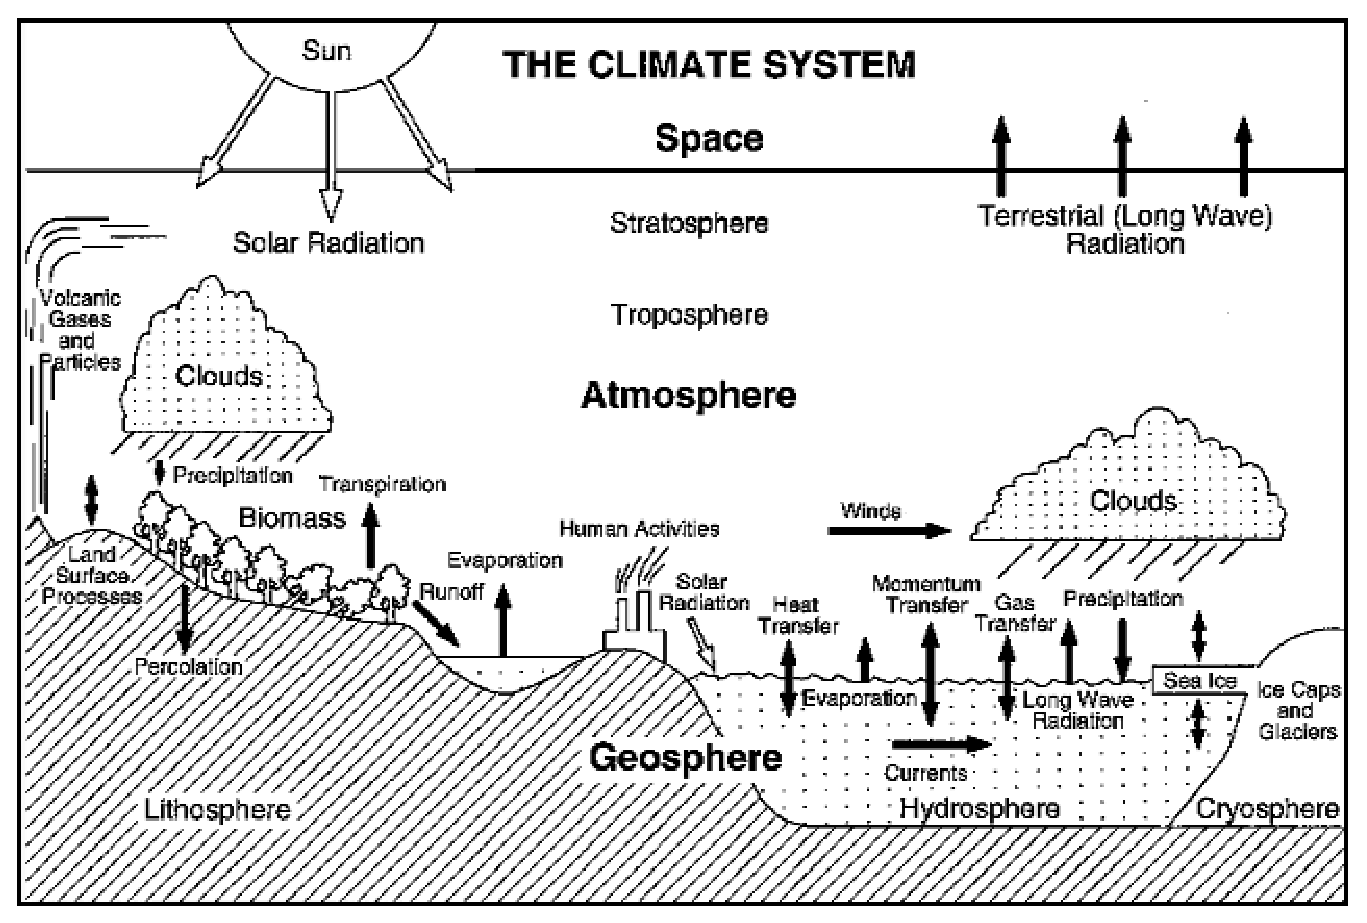
\includegraphics[height=6.0cm]{ambsthermopict/climate.eps} 
} 
\caption{Global heat balance.}
\label{nse_people} 
\end{figure}


\section{Black Body Radiation and the Sun}


A \emph{black body} absorbs incoming white light of all frequencies, 
from high frequency ultraviolet to low frequency infrared, but only radiates
low frequency light (with color depending on 
the temperature of the body).  This is the basis of the gross energy balance
of the Earth absorbing white light from the hot Sun and radiating 
low frequency light into empty space. One can view  
black body absorption/emission as an (irreversible) 
thermodynamic process transforming high frequency light energy  
to low frequency (long wave) light energy \cite{blackbody}. 


\begin{figure}[bhpt] 
\centerline{ 
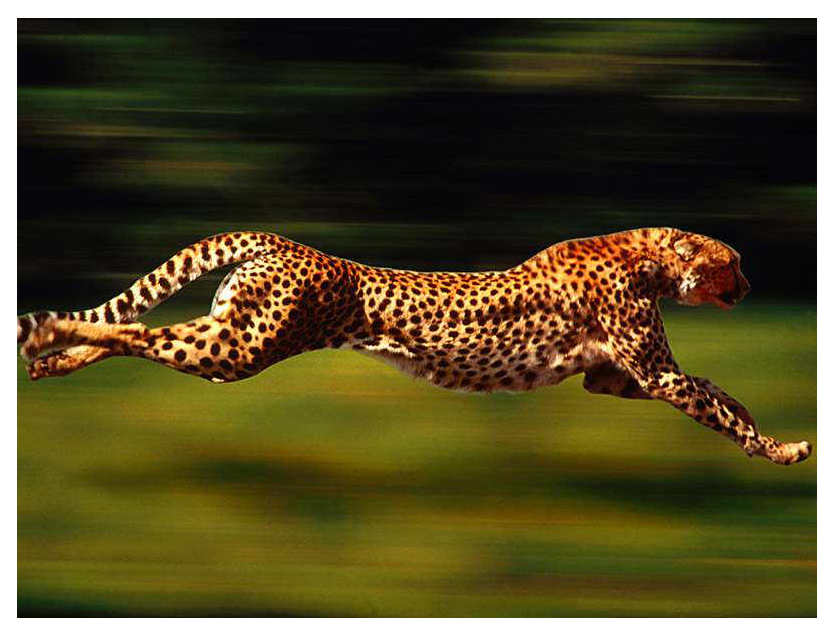
\includegraphics[height=6.0cm]{ambsthermopict/gepard.eps} 
} 
\caption{Life in action.}
\label{nse_people} 
\end{figure}


\begin{figure}[bhpt] 
\centerline{ 
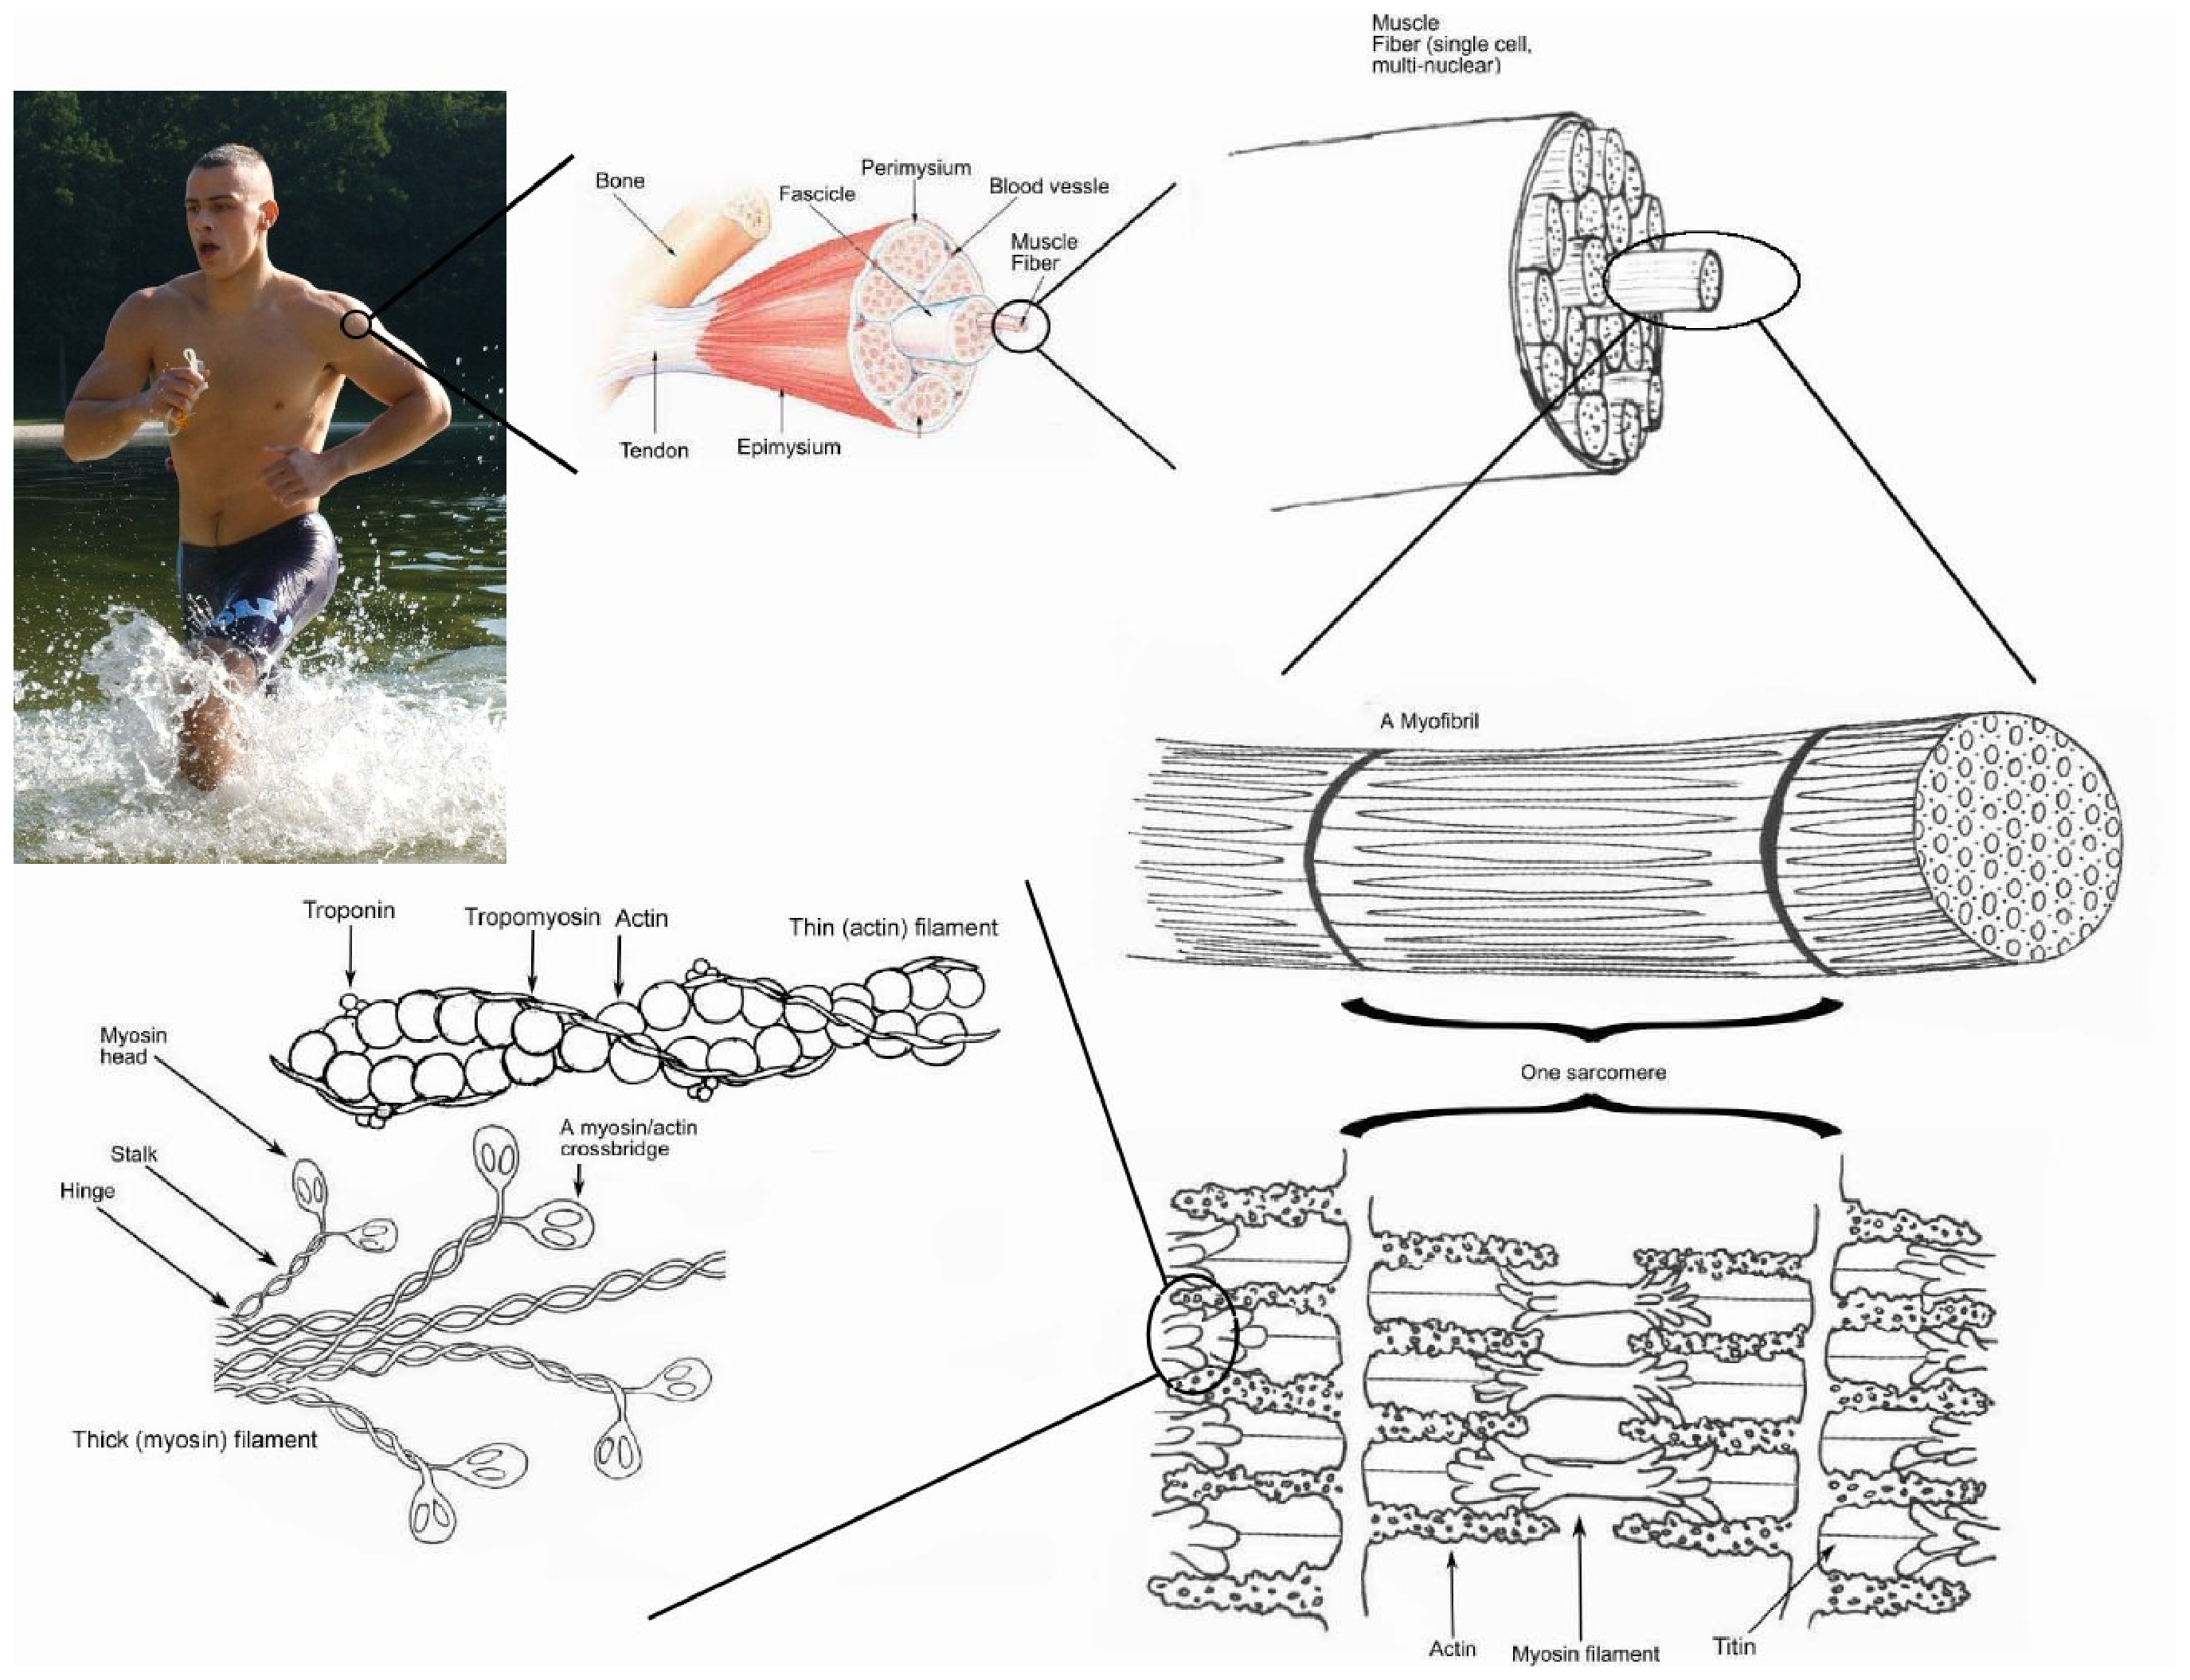
\includegraphics[height=8.5cm]{ambsthermopict/muscle.eps} 
} 
\caption{Muscle contraction by actin-myosin twitch fueled by ATP.}
\label{nse_people} 
\end{figure}




\section{Biology and Life}

Most forms of biological processes build on conversion of
chemical energy into heat and kinetic energy,
and thus ultimately on Solar energy converted to chemical energy 
in the \emph{photo-synthesis}.


\emph{Muscle contraction}  
occurs when a muscle fiber generates tension through
\emph{actin and myosin cross-bridge cycling} shortening the fiber
fueled by \emph{Adanenosine TriPhosphate ATP}.
Locomotion in most higher animals is possible only 
through the repeated contraction of many muscles at the correct times 
controlled by the central nervous system,
the brain and spinal cord. Voluntary muscle contractions 
are initiated in the brain, while the spinal cord initiates involuntary 
reflexes.

The emergence of biological life may naively appear to contradict the 2nd 
Law in its classical form, by creating ordered structures out of disordered, 
while the death of a living organism when order dissolves into disorder,
reflects the classical 2nd Law very well. We shall see that in the
new formulation of the 2nd Law not relying on notions of 
ordered/unordered, there
is nothing (in principle) that prevents ordered structures to develop 
from unordered
(for example in Irak), assuming there is some input of energy (oil). 
%which is kind of a happy message to everybody who is not an extreme pessimist.
%This is one of many indications that
%the classical from of the 2nd Law poses
%difficulties.

\begin{figure}[bhpt] 
\centerline{ 
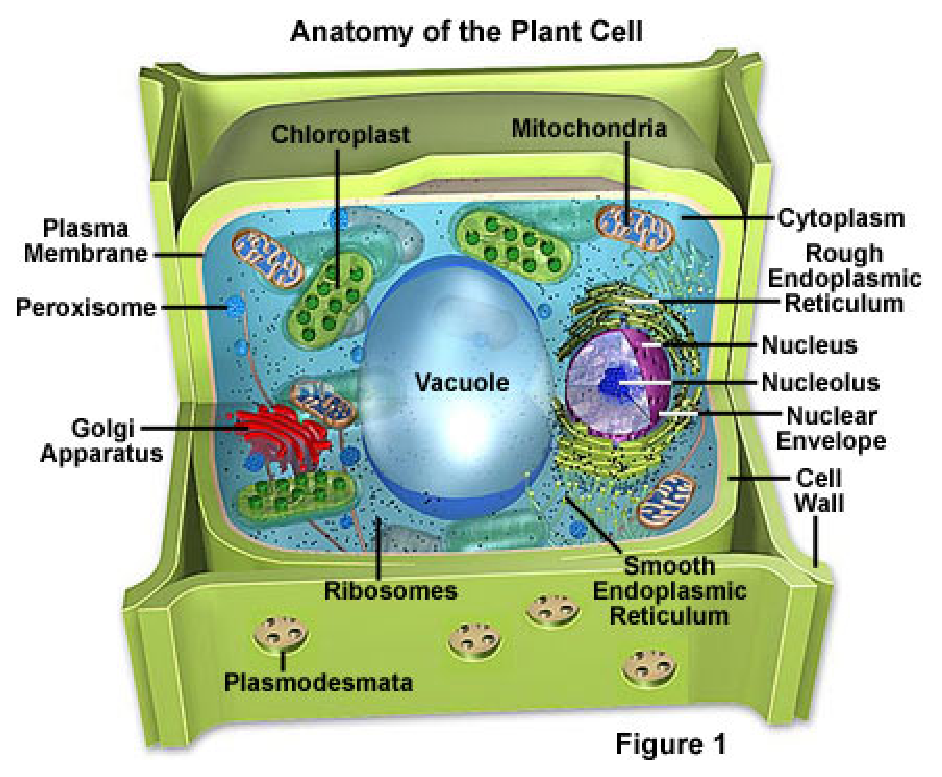
\includegraphics[height=6.0cm]{ambsthermopict/plantcell.eps} 
} 
\caption{Inside a plant cell.}
\label{nse_people} 
\end{figure}


\section{Molecular Biology and Protein Folding}

Biology builds on cell microbiology based on the thermodynamics of
chemical reactions of \emph{protein
synthesis} from amino acid molecules according to
the instructions of \emph{DNA}. Computational thermodynamics of the cell
is becoming an increasingly important tool in medicine and drug design.

%\begin{figure}[bhpt] 
%\centerline{ 
%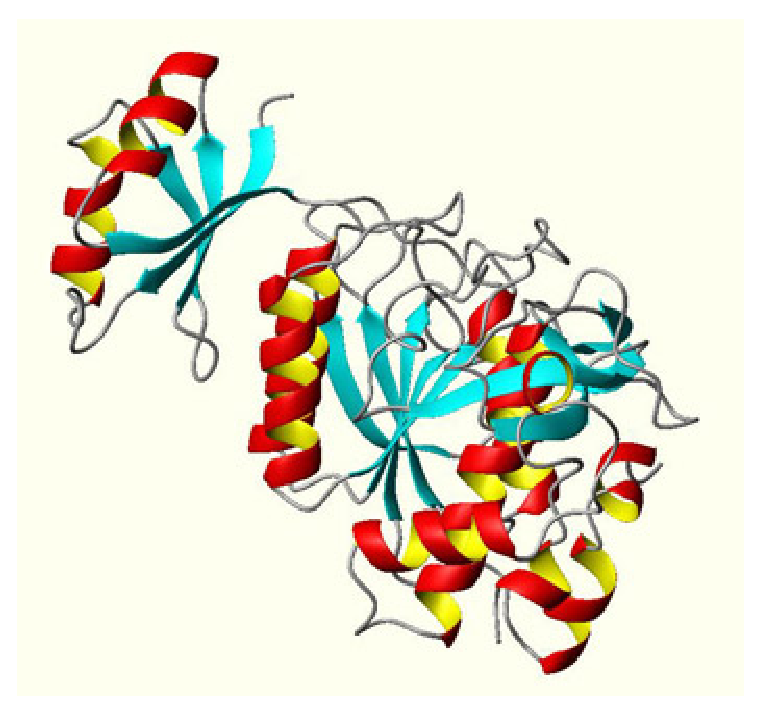
\includegraphics[height=8.0cm]{ambsthermopict/proteinfolding.eps} 
%} 
%\caption{Protein folding}
%\label{nse_people} 
%\end{figure}

%\begin{figure}[bhpt] 
%\centerline{ 
%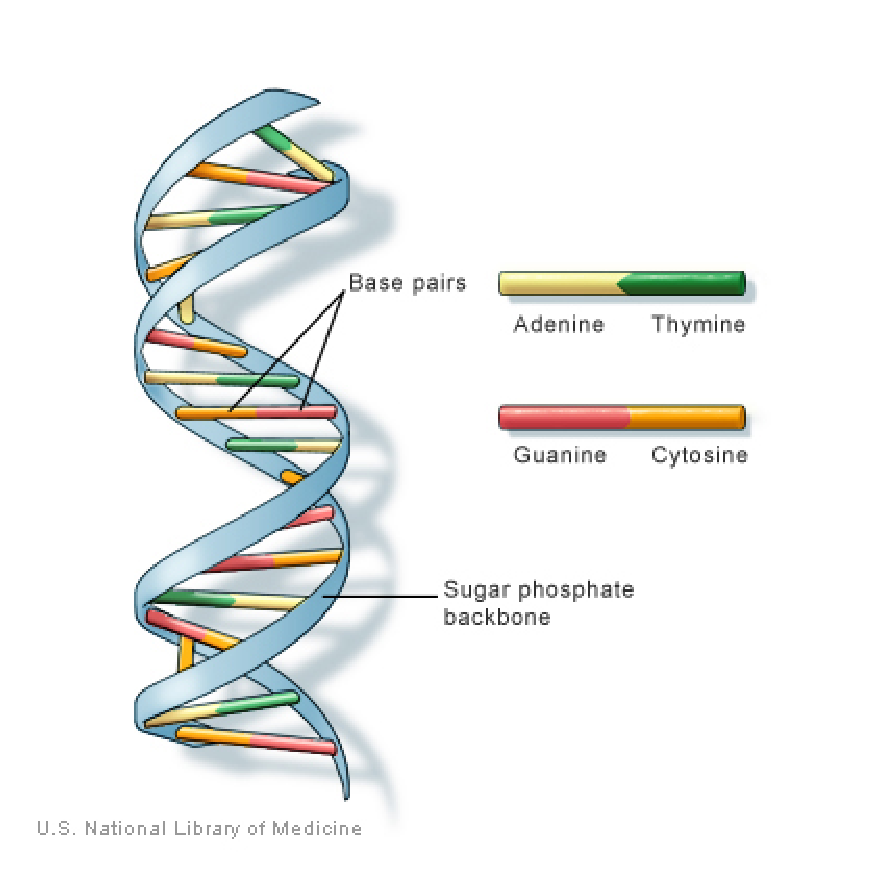
\includegraphics[height=8.0cm]{ambsthermopict/doublehelix.eps} 
%} 
%\caption{The double helix of DNA}
%\label{nse_people} 
%\end{figure}



 
\section{Quantum Physics and Chemistry}

The thermodynamics of chemical reactions and radiation
build on the \emph{quantum mechanics}
of electrons, and the thermodynamics of nuclear reactions build
on quantum electrodynamics of elementary particles. Computational solution
of the equations of quantum mechanics presents a tough challenge, 
because of the richness of the the wave function solution 
with in principle three independent 
space coordinates for each particle (electron) involved. 
Methods
reducing the dimensionality are today routinely used in massive
computations in \emph{quantum chemistry}, and could open to new insights
of the nature of the quarks of elementary particle physics.
%\cite{compquantum}. 

 




\section{Energy Generation and Consumption}

Our \emph{industrial society} is based on production and
consumption of energy in thermodynamic energy conversion processes of 
the form:

\begin{itemize}

\item nuclear/fossile/biological/chemical $\rightarrow$ heat/kinetic/electric, 

\item wind/wave kinetic $\rightarrow$ electric,

\item solar radiation $\rightarrow$ heat/electric.
\item electric $\rightarrow$ heat/kinetic.  
\end{itemize}
In all conversion of energy, minimization of \emph{losses} into useless heat is 
of prime concern, for which computational thermodynamics opens new
possibilities.
\section{Heat Engines and Industrialization}

%The early development of thermodynamics was motivated by the need of 
%understanding the steam engine, underlying the industrialization
%of the Western World in the 19th century.

The industrial society
of the 19th century was built on the use of \emph{steam engines}, and the 
initial motivation to understand thermodynamics came from a need to
increase the efficiency of steam engines for conversion of heat energy to
useful mechanical energy. 
\begin{figure}[bhpt] 
\centerline{ 
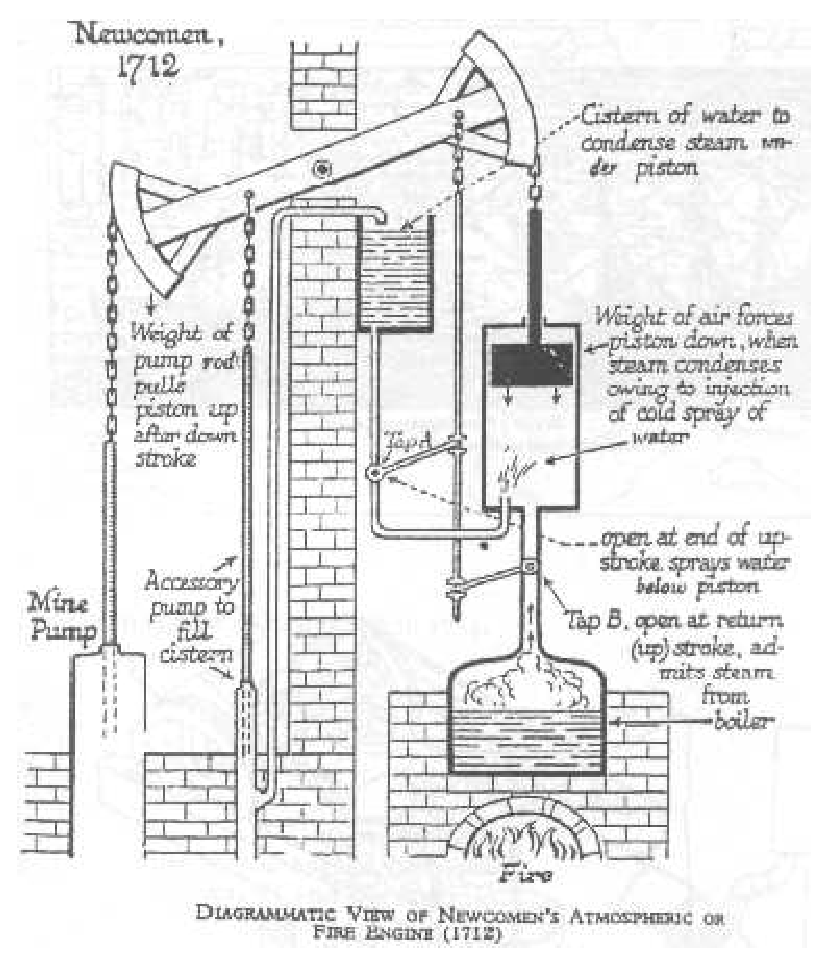
\includegraphics[height=10.0cm]{ambsthermopict/newcdiag.eps} 
} 
\caption{Converting heat to kinetic (mechanical) energy in 1712.}
\label{nse_people} 
\end{figure}  
A steam engine
is a particular form of a 
\emph{heat engine} converting heat to mechanical work in a thermodynamical
process. The modern \emph{combustion engine} in a car 
is a form of heat engine generating kinetic energy
from explosive burning of fuel.
 The efficiency of a heat engine is of 
prime importance, and can be studied by computational thermodynamics.
The necessary \emph{cooling} of a car engine represents 
a loss of energy which is not transformed into useful mechanical work.  

\section{Heat Pumps and Oil Crisis}

The \emph{heat pump} is replacing the increasingly expensive oil
for heating of houses. A heat pump converts low temperature heat energy
from the earth or the air to higher temperature useful heat energy, by
supplying the necessary conversion energy from electricity.
The efficiency is today typically around $2/3$, that is, for $1/3$
unit of electric energy, you get out 1 unit of useful heat energy. 
You can thus reduce your electrical bill by a factor of $3$ by
changing from full electrical heating of your house 
to heating by an efficient heat pump. Of course, it is of interest 
to seek to increase the efficieny even more. Can we reach $99\%$ 
efficiency, and if not why? We will address this question below.

\section{Refrigerators and Urban Civilization}

A \emph{refrigerator} is a form of heat pump taking heat from
the inside of the refrigerator and delivering it to the exterior at
higher temperature. 
The refrigerator is an absolute necessity of modern urban civilization.

The standard design builds on cycling a fluid alternating
between \emph{expansion/evaporation} to gas phase with temperature drop, and 
\emph{compression/condensation} to liquid phase with temperature increase,
with the cold gas in contact with the interior of the refrigerator 
and the warm liquid phase in contact with the exterior.
The cooling process with heat flowing from
cold to hot (contrary to its natural tendency to flow from hot to cold)
is thus maintained by an (electric) \emph{compressor} 
consuming energy.

\begin{figure}[bhpt] 
\centerline{ 

\includegraphics[height=6.0cm]{ambsthermopict/refrigerator.eps} 
} 
\caption{Inside a refrigerator: The principle of preservation of food.}
\label{nse_people} 
\end{figure}




The first design of an \emph{absorption refrigerator}, without compressor and
moving parts and thus silent,
was invented by the two young Swedish
engineering students Carl Munters and Baltzar von
Platen during their class in 
thermodynamics at the Royal Institute of Technology in 1922
(although they slept through the lectures working all night
on their invention).
This invention together with a vacuum cleaner
gave the impetus of the quick expansion of the Electrolux company.
The production of the Munters-Platen refrigerator has 
continued at Motala in Sweden uninterrupted
since 1925 with today a total of 10 million units being produced. 
We hope this book may be useful for young minds of today
for new inventions.


\section{Information and Communication}

\emph{Information theory} was created by Shannon \cite{shannon} in 
the 1940s borrowing the concept of \emph{entropy} from 
\emph{thermodynamics}, with the idea of measuring  
communication channel capacity requirements for different types of information.
Random information would then represent information with
maximal entropy, in principle requiring maximal capacity
(although random information would seem like useless information). 
 
Alternatively, one can view communication of information as a 
thermodynamic flow with the heat energy
representing loss or destruction of information during the communication.
More generally, not only creation but also destruction 
of information represent fundamental aspects of 
physical and biological processes.

\begin{figure}[bhpt] 
\centerline{ 
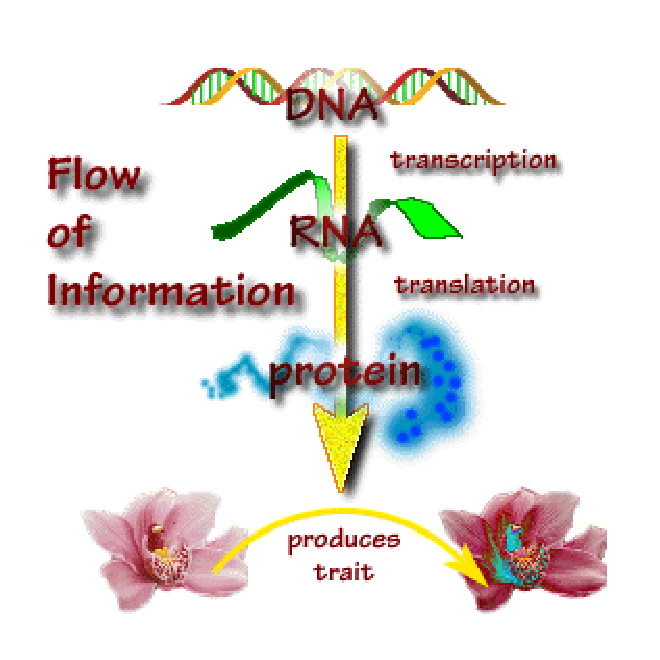
\includegraphics[height=6.0cm]{ambsthermopict/GPFlowInfo.eps} 
} 
\caption{Flow of information in a flower.}
\label{nse_people} 
\end{figure}



\section{Economy and Welfare}

One can also view an evolving economy as a 
thermodynamic flow process transforming resources into utilities.
In (a free) economy turbulent dissipation could be viewed as a measure
of necessary losses during the process, in the form of interest rates,
taxes, bribes, 
thefts, which cannot (fully) be avoided. The flow of the World economy 
represents a complex process of prime importance to all of us.
An economist with (some) understanding of the process can be raised to 
fame and fortune.  

\begin{figure}[bhpt] 
\centerline{ 
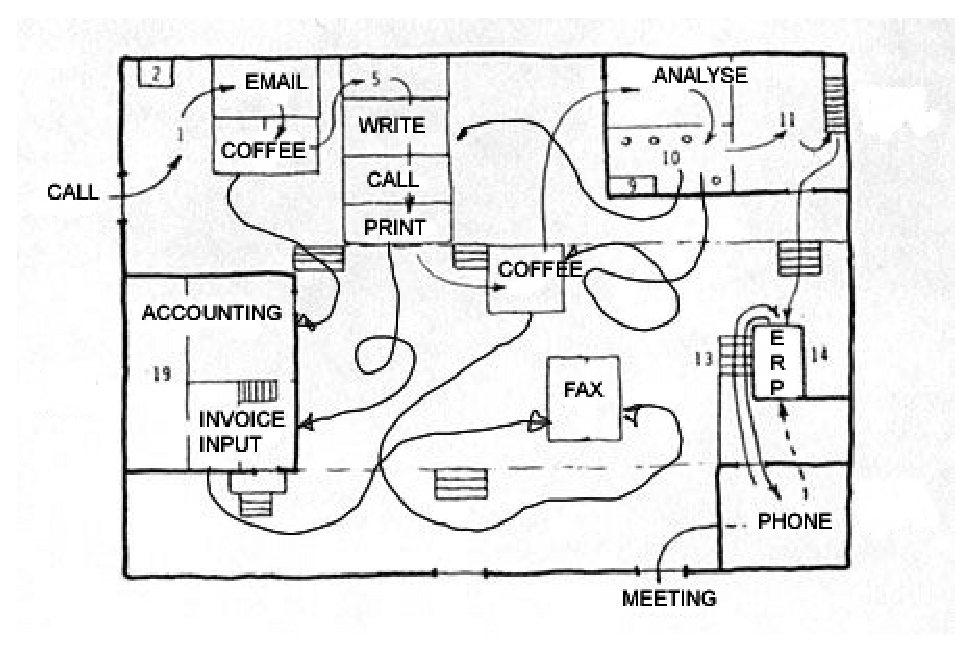
\includegraphics[height=6.0cm]{ambsthermopict/brainshopflow.eps} 
} 
\caption{Flow of information in an office of the last century.}
\label{nse_people} 
\end{figure}

\section{Emergence: A New Approach to Physics}

Ilya Prigogine received the Nobel Prize in Chemistry in 1977
for his work on \emph{non-equlibrium thermodynamics} proposing
a new (statistical) approach to the 2nd Law
allowing ordered structures to develop from non-ordered, see  
%\hyperref[ilyaworld]{Fig. \ref{ilyaworld}} and \ref{ilya}.
Fig. \ref{ilyaworld} and \ref{ilya}.
Even if Prigogine did not convince the physics
community at large, he at least showed the severe short-coming 
of the classical 2nd Law seemingly preventing order from
develping from chaos.

\emph{Emergence} is the process of complex pattern formation
from more basic constituent parts or ``particles'', that is the formation
of order out of chaos. Turbulence shows phenomena of both emergence
and featureless chaos, none of which can be understood by considering only
a single fluid particle, only by considering the interaction of many.
The (new) 2nd Law expresses a collective behavior of many 
fluid particles to form turbulent flow with an 
irreversible transfer of large scale kinetic energy to 
heat energy. Thus thermodynamics
naturally connects to the new approach to physics 
based on emergence, which is now
developing (emerging) 
with input from e.g. 1988 Nobel Laurate Robert Laughlin \cite{laughlin}, 
and which is
radically different from the \emph{reductionist} approach of elementary
particle physics completely dominating the scene since the 
birth of quantum mechanics in the beginning of the last century.

Since emergence concerns the interaction of many particles, analytical
methods fall short (which lies behind the reductionist
obsession with a single particle
hopefully allowing analytical mathematical description),
while computational methods open new possiblities of simulating
emergent and turbulent phenomena, as is shown in this book.


\begin{figure}[bhpt] 
\centerline{ 
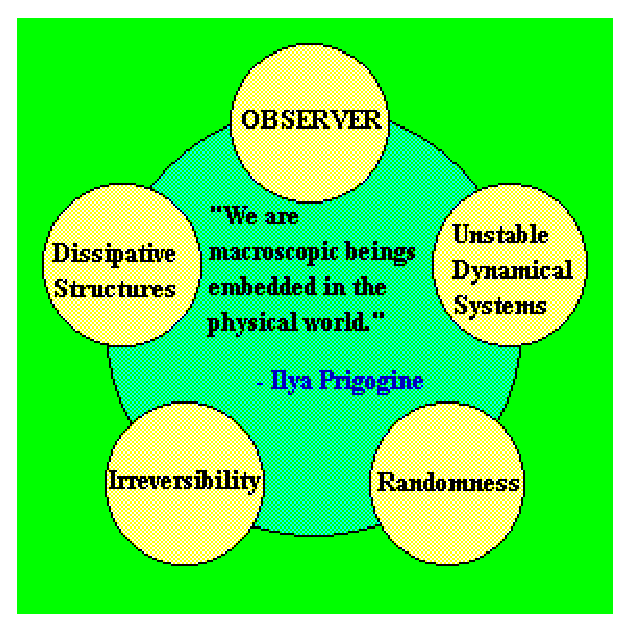
\includegraphics[height=8.0cm]{ambsthermopict/ilyaflow.eps} 
} 
\caption{The World according to Ilya Prigogine.}
\label{ilyaworld} 
\end{figure}\begin{figure}[bhpt] 
\centerline{ 
\includegraphics[height=8.0cm]{ambsthermopict/prigogine.eps} 
} 
\caption{Ilya Prigogine receiving the Nobel Prize in Chemistry
in 1977 from the hands of King Karl XVI Gustav.}
\label{ilya} 
\end{figure}

\section{The Battle between Growth and Decay}

We shall see that turbulent flow and thus thermodynamics (the World)  
can be viewed as a battle between a growth process of \emph{differentiation
by advection} and a decay process of \emph{mixing by diffusion} according
to:
\begin{itemize}
\item \emph{growth: increase difference-differentiate-separate: advection}
\item \emph{decay: decreasse difference--uniformize-mix: diffusion.}
\end{itemize} 
The classical 2nd Law captures the diffusion process with mixing
and decreasing difference. But it does not capture the 
advection process allowing increasing difference and separation,
which is a severe short-coming. The new 2nd Law captures
both processes. In the thermodynamics of Prigogine the two processes are
represented  by ``Unstable Dynamical Systems'' and ``Dissipative Structures'',
but Prigogine sticks to ``Randomness'', see Fig. \ref{ilyaworld}.


\section{Physics: Flow of Information: Computation}

The basic idea of this book 
is to view thermodynamics as a form of 
analog computation, which can be simulated by digital computation. 
Both analog physics and digital computation can be seen as  
flows of information reflecting the flow of mass, momentum and 
energy in a physical system and the flow of digits from input to output in the
execution of a subroutine of the computational code.

For a computer programmer the information flow is 
represented in the flow chart of a computer code, which
is essential for the understanding of the code. 
Likewise, a flow chart of the analog computation 
of a physical process can help the physicist 
to understanding.



 
\section{Thermodynamics as a ``Best of  Worlds''}

The above survey indicates that thermodynamics 
is a fundamental part of science and
technology and thus serves a very important role in our society.
Thermodynamics is maybe the scientific field closest to 
Leibniz' definition of a \emph{Best of Worlds}
as a world, which is richest in variation of ordered complex
structures or emergence, such as different forms of life and conscience,
while being governed by simplest possible principles or laws.



\small
\begin{quote}I say that I am strongly inclined to believe that heat is of 
the same kind, and that material things which make us hot and feel hot 
(such as we call by the general name \emph{fire} are a multitude of tiny 
corpuscles of such and such a shape, and moving at such and such a speed. 
When they meet our bodies, they penetrate them with their extreme subtlety, 
and the way they touch our substance as they pass through it is sensed by 
us as the affection we call ``heat''. 
It is pleasant or unpleasant in 
proportion to the number and speed of the particles as they prick and 
penetrate it. This penetration is pleasant if it is beneficial to our 
insensible vital functions, and unpleasant when it causes too much of a 
separation and dissolution of our substance. (Galieo in \emph{The Assayer}, 
1623)
\end{quote}
\normalsize




\fi  % --- end moved Transformations of Energy block ---

\iffalse  % --- removed in shortened layout: duplicate of earlier "Classical Thermodynamics" chapter + redundant 2nd-Law revisit ---
\chapter{Classical Thermodynamics}
\label{chapter:dice}

\small

%\begin{quote}...the whole procedure was an act of despair because a
%theoretical interpretation had to be found at any price, no matter
%how high that might be... (Planck on the statistical mechanics basis of 
%his radiation law)
%\end{quote}
%\begin{quote} Where does irreversibility come from? It does not come
%form Newton's laws. Obviously there must be some law, some
%obscure but fundamental equation. perhaps in electricty,
%maybe in neutrino physics, in which it \emph{does}
%matter which way time goes. (The Feynmman Lectures on Physics 1963)
%\end{quote}
%\begin{quote} The 2nd Law cannot be derived from purely mechanical
%laws. It carries the stamp of the essentially statitical nature of heat.
%(Bergman in Basic Theories of Physics 1951)
%\end{quote}

%\begin{quote} Vether it's worth goin' through so much, to learn
%so little, as the charity-boy said ven he got to the end of the
%alphabet, is a matter o'taste. (Charles Dickens in Pickwick Papers)
%\end{quote}

%\begin{quote} Everyone knows that heat can produce motion. That it possesses
%vast motive power no one can doubt, in these days when the steem engine is 
%everywhere so well known. The study of these enegines is of great interest,
%their importance is enormous, their use is contnually increasing, and they
%seem desined to produce a great revolution in the civilized world.
%(Carnot \cite{carnot} 1824).
%\end{quote}
%\begin{quote} 
%The total energy of the universe is constant; the total entropy is 
%continually increasing. (Rudolf Clausius 1865)
%\end{quote}
\begin{quote}
Neither Herr Boltzmann nor Herr Planck has given 
a defnition of $W$...
Usually $W$ is put equal to the number of complexions. In order
to calculate $W$, one needs a \emph{complete} (molecular-mechanical) 
theory of the system under consideration. Therefore it is dubious 
whether the Boltzmann principle has any meaning without a 
\emph{complete} molecular-mechanical
theory or some other theory which describes the elementary processes (and such
a theory is missing). (Einstein)
\end{quote}
\begin{quote} The reversibility of the mechanical theory suggested for
many years that any observable motion should have a twin reverdes
motion which can also be observed. The consequences of reversibility,
however, seem contrary to our intuition: Although salt spontaneously
dissolves in water, no one has ever seen salt precipitate from an
unsaturated solution. (Joel Keizer in \emph{Statistical Thermodynamics
of Nonequilibrium processes})
\end{quote}
\begin{quote} Mechanically, the task seems impossible, and we will just
have to get used to it (statistics of quanta) (Planck 1909).
\end{quote}
\normalsize


\section{The 1st and 2nd Laws of Thermodynamics}

The development of classical thermodynamics was initiated in 
the 19th century by Carnot \cite{carnot}, Clausius 
\cite{clausius1,clausius2} and Lord Kelvin \cite{kelvin}, who formulated
basic axioms in the form of the \emph{1st Law} and the \emph{2nd Law} of
thermodynamics. 
%The 1st Law states (for an isolated system)
%that the \emph{total energy}, the sum of kinetic and heat energy, is conserved.
%The 1st Law is naturally generalized to include also conservation 
%of mass and Newton's law of conservation of momentum and thus
%the 1st Law expresses \emph{conservation of mass, momentum and total energy}.
%For an \emph{ideal} gas/fluid with vanishing viscosity and heat conductivity,  
%the 1st Law takes the form of the \emph{Euler equations}
%which formally can be viewed as a \emph{Hamiltonian system}.
%The 1st law can be viewed as a definition, with any loss of kinetic 
%energy defined to be heat energy.
%\section{The Classical Laws of Thermodynamics}
The 1st Law states conservation of total energy 
as the sum of kinetic, potential and heat energy. The 1st Law 
can be viewed as a definition of heat energy as
any loss of kinetic/potential energy in conserved total energy. 
The classical 2nd Law has several forms from the formulation
by Carnot in terms of \emph{heat engines} to that by Clausius
in terms of entropy:


\begin{itemize}


\item Carnot 1824: \emph{No heat engine can be more efficient than a 
Carnot engine with efficiency
$1-t_c/t_h$ operating between two temperatures $t_h$ and $t_c<t_h$}. 

\item Clausius 1850: \emph{It is impossible for heat to flow from a colder body
to a warmer body without any work having been done to accomplish the flow. 
Energy will not flow spontaneoulsy from a low temperature object to
a higher temperature object}.
 
\item Kelvin-Planck 1851 \cite{kelvin}: 
\emph{It is impossible to obtain a process that, operating in cycle, produces no 
other effect than the subtraction of a positive amount of heat from a 
reservoir and the production of an equal amount of work}.

\item Clausius 1865: \emph{In any cyclic process the entropy cannot decrease}.
\end{itemize}
Clausius', Kelvin-Planck's and Carnot's formulations are negative
and express 
impossibilitities, which are tricky to dechiffer: If somebody claims having  
constructed an engine more efficient than a Carnot engine, then Carnot
would say that it is not a heat engine. Or if we observe heat flow
from a cold to a warm body (which we will do below), 
then Clausius would say that it is not spontaneous and Kelvin-Planck
that some other effect must have been produced. 
%We understand 
%that in the end this runs the risk of being  an empty play with words,
%where a heat engine is an engine which is not more efficient
%than a Carnot engine and spontaneous heat flow (from warm to cold)
%can only occur spontaneously.

The only statement of the above versions of the 2nd Law
 which is positive in form,
is the last one about entropy.  But this formulation requires a 
specification of the physical significance of entropy,
and this has shown to be very difficult, if not 
impossible to achieve. In particular, nobody has found
any sensor of entropy in Nature,  and the physical mechanism 
preventing entropy from decreasing has remained mysterious.

\begin{figure}[bhpt] 
\centerline{ 
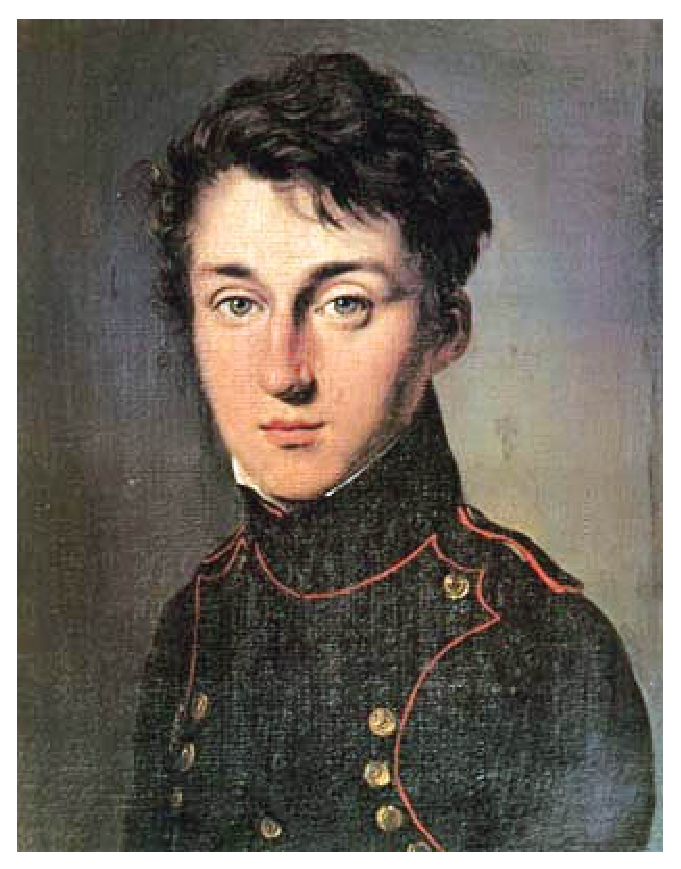
\includegraphics[height=8.0cm]{ambsthermopict/Carnot.eps} 
} 
\caption{Sadi Carnot: \emph{No heat engine can be more efficient than a 
Carnot engine.}}
\label{nse_people} 
\end{figure}

\begin{figure}[bhpt] 
\centerline{ 
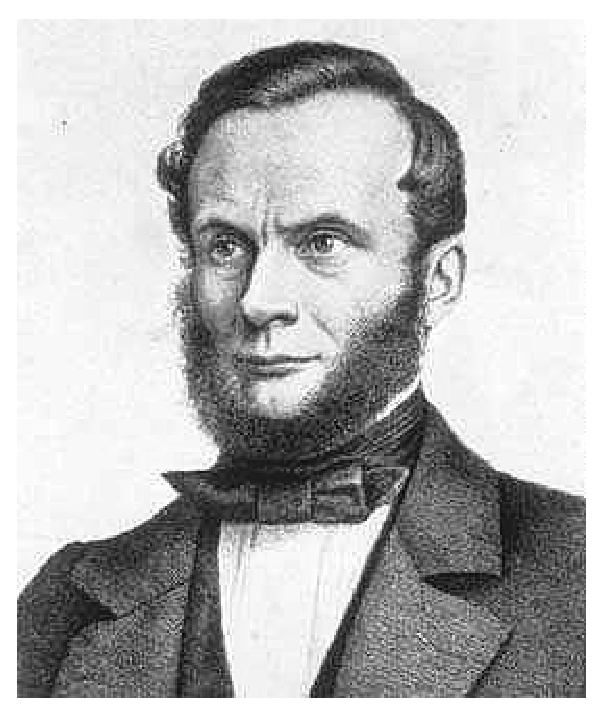
\includegraphics[height=8.0cm]{ambsthermopict/clausius.eps} 
} 
\caption{Rudolf Clausius: \emph{The energy of the world is 
constant. Its entropy tends to a maximum.}}
\label{nse_people} 
\end{figure}


\begin{figure}[bhpt] 
\centerline{ 
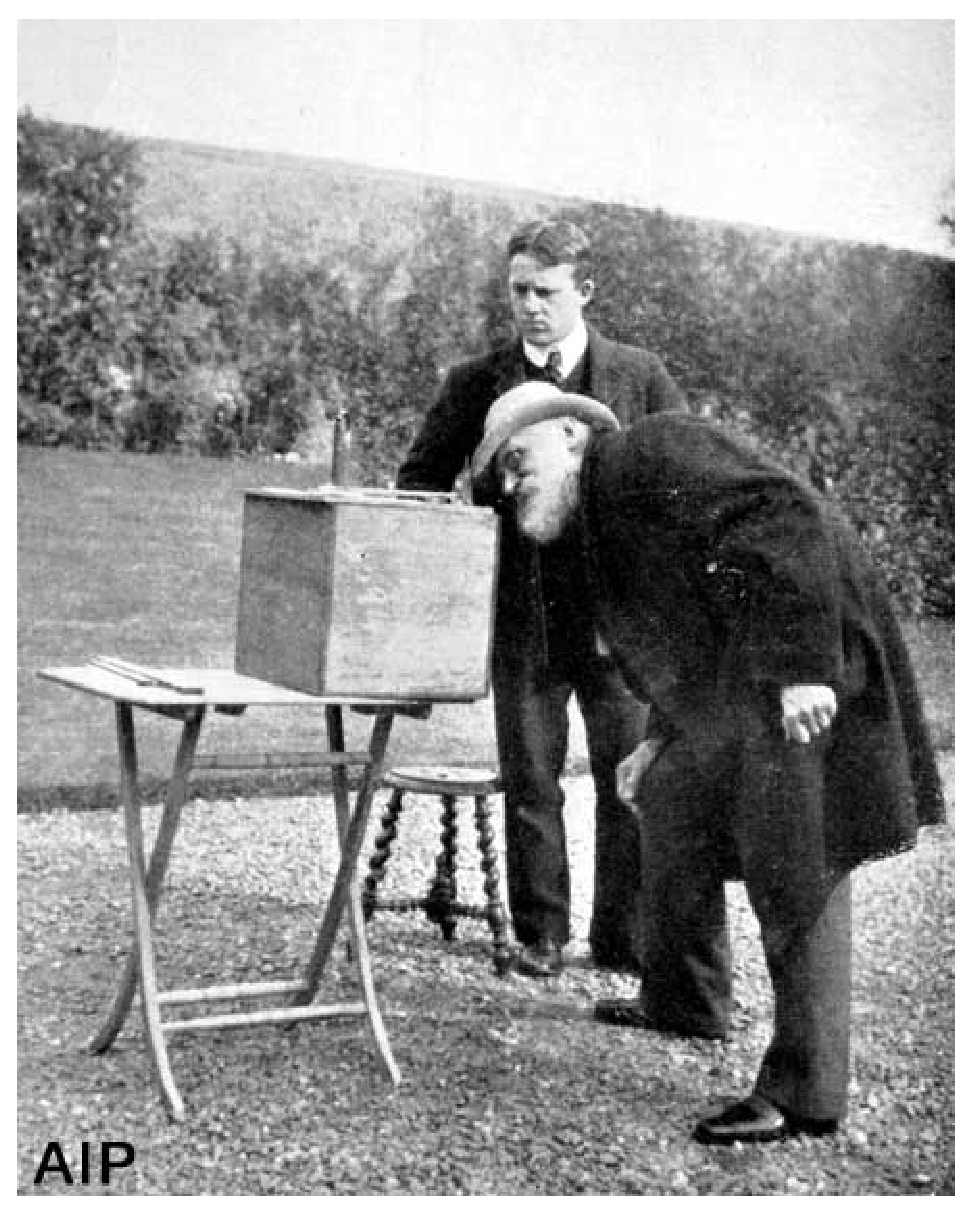
\includegraphics[height=16.0cm]{ambsthermopict/kelvin_assistant.eps} 
} 
\caption{Lord Kelvin to assistent while making observations:
\emph{I am never content until I have constructed a mechanical model of what I am studying. If I succeed in making one, I understand; otherwise I do not.}}
\label{nse_people} 
\end{figure}

To give perspective we recall the presentations of thermodynamics
and statistical mechanics from the standard source Wikipedia representing
a form of common understanding as of today.



\section{Thermodynamics in Wikipedia}


\emph{Thermodynamics (from the Greek thermos meaning heat and dynamis 
meaning power) 
is a branch of physics that studies the effects of changes in temperature, 
pressure, and volume on physical systems at the macroscopic scale by 
analyzing the collective motion of their particles using statistics. 
Roughly, heat means "energy in transit" and dynamics relates to "movement"; 
thus, in essence thermodynamics studies the movement of energy and how 
energy instills movement. Historically, thermodynamics developed out of 
the need to increase the efficiency of early steam engines}.

\emph{The starting point for most thermodynamic considerations are the laws of 
thermodynamics, which postulate that energy can be exchanged between 
physical systems as heat or work. They also postulate the existence of a 
quantity named entropy, which can be defined for any system. 
In thermodynamics, interactions between large ensembles of objects are 
studied and categorized. Central to this are the concepts of system and 
surroundings. A system is composed of particles, whose average motions 
define its properties, which in turn are related to one another through 
equations of state. Properties can be combined to express internal energy 
and thermodynamic potentials are useful for determining conditions for 
equilibrium and spontaneous processes}.

\emph{With these tools, thermodynamics describes how systems respond 
to changes 
in their surroundings. This can be applied to a wide variety of topics in 
science and engineering, such as engines, phase transitions, chemical 
reactions, transport phenomena, and even black holes. The results of 
thermodynamics are essential for other fields of physics and for 
chemistry, chemical engineering, cell biology, biomedical engineering, 
and materials science to name a few}.




\begin{figure}[bhpt] 
\centerline{ 
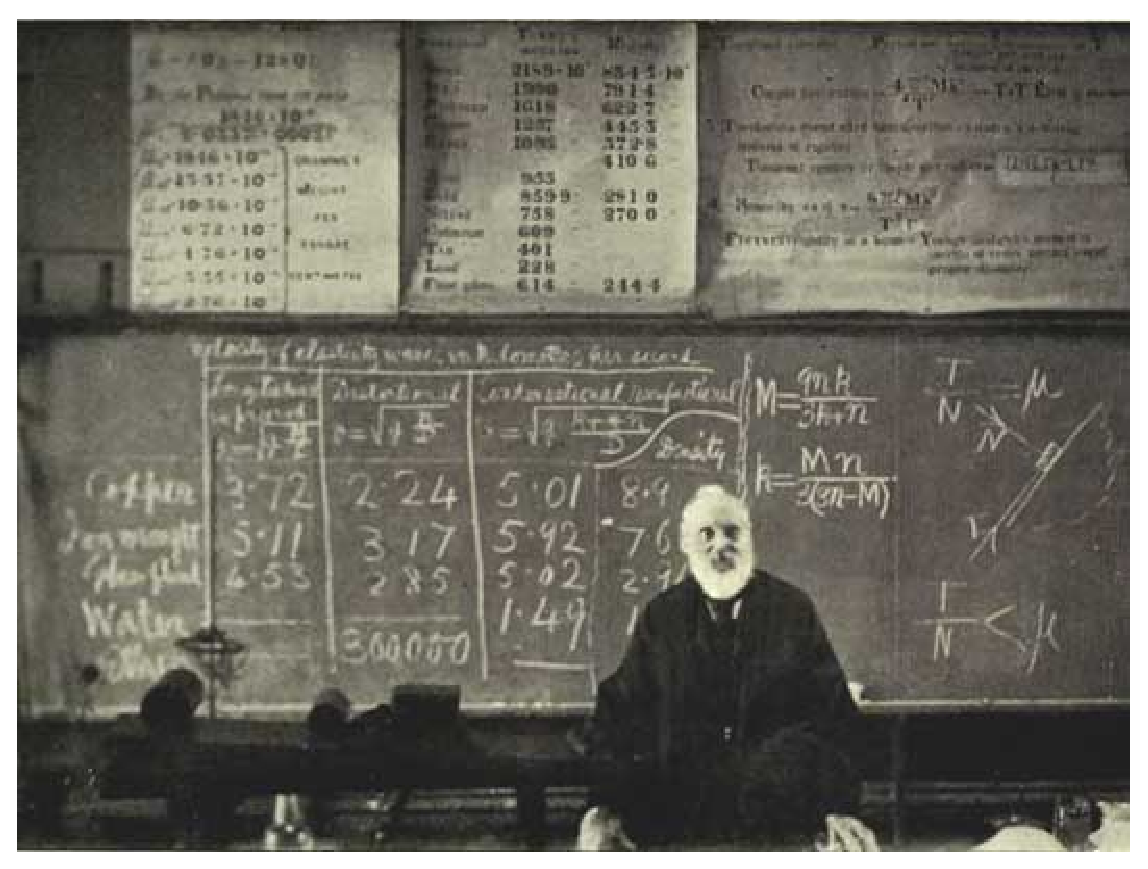
\includegraphics[height=10.0cm]{ambsthermopict/kelvinlecture.eps} 
} 
\caption{Lord Kelvin in his last lecture: \emph{Do not imagine 
that mathematics 
is hard and crabbed, and repulsive to common sense. It is merely the 
etherialization of common sense.}}
\label{nse_people} 
\end{figure}




\section{Statistical Mechanics in Wikipedia}


\emph{Statistical mechanics is the application of statistics, which includes 
mathematical tools for dealing with large populations, to the field of 
mechanics, which is concerned with the motion of particles or objects 
when subjected to a force}.

\emph{It provides a framework for relating the microscopic properties of 
individual atoms and molecules to the macroscopic or bulk properties 
of materials that can be observed in everyday life, therefore explaining 
thermodynamics as a natural result of statistics and mechanics 
(classical and quantum) at the microscopic level. In particular, it can 
be used to calculate the thermodynamic properties of bulk materials 
from the spectroscopic data of individual molecules}.

\emph{This ability to make macroscopic predictions based on microscopic 
properties is the main asset of statistical mechanics over thermodynamics. 
Both theories are governed by the second law of thermodynamics through 
the medium of entropy. However, Entropy in thermodynamics can only be 
known empirically, whereas in Statistical mechanics, it is a function 
of the distribution of the system on its micro-states}.
\normalsize

\begin{figure}[bhpt] 
\centerline{ 
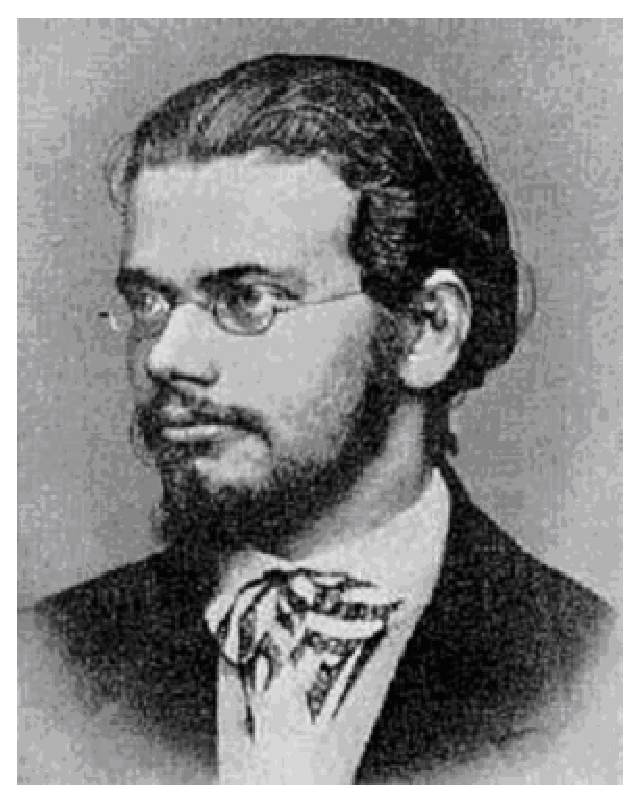
\includegraphics[height=8.0cm]{ambsthermopict/Boltzmann.eps} 
} 
\caption{Ludwig Boltzmann: \emph{Available energy is the main object at stake in the struggle for existence and the evolution of the world.}}
\label{nse_people} 
\end{figure}



\begin{figure}[bhpt] 
\centerline{ 
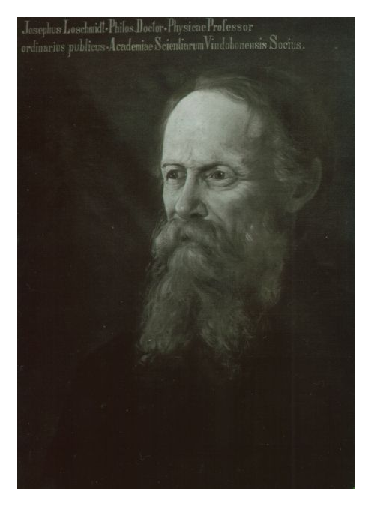
\includegraphics[height=8.0cm]{ambsthermopict/loschmidt.eps} 
} 
\caption{Loschmidt: \emph{I consider irreversibility in reversible systems
to be paradoxical. Indeed very paradoxical, yes.}}
\label{nse_people} 
\end{figure}


\section{The 2nd Law in Popular Science}  
  
%Popular science can be a good source when seeking to find the weak
%point of a scientific theory, because the usual safe-guards of
%scientific hype can be lowered when addressing a (not so critical) 
%general public.  
In \emph{The Cosmic Blueprint} by the physicist Paul Davies,
we read on statistical mechanics and the 2nd Law: 


\begin{itemize}
\item \emph{One of the states will represent ``maximal disorder'',
which is the state attainable in a maximal number of ways, or the 
macro-state with a maximal number of corresponding micro-states.}
\item \emph{The maximally disordered state thus corresponds to
thermodynamic equilibrium.}
\item \emph{One can define a statistical quantity representing
the ``degree of disorder'' of a (macro)state, in terms of the number
of corresponding microstates.}
\item \emph{Boltzmann showed that if the molecular collisions 
are chaotic (in a rather precise sense), this quantity will
with an overwhelming probability increase.}
\item \emph{Boltzmann had thus found a quantity in statistical mechanics
corresponding to thermodynamic entropy.}
\item \emph{Boltzmann thus gave a demonstration, at least in
a simple gas model, of ``why'' entropy tends to increase.}   
%\item \emph{In the deterministic Newtonian world there is no arrow
%of time. Boltzmann found an arrow hidden in the molecular roulette
%game of Nature.}
\end{itemize}
Davies description illustrates that there are two different notions
of entropy and two corresponding versions of the 2nd Law, 
one in classical thermodynamics and one in statistical
mechanics. The 2nd Law in classical thermodynamics is usually 
considered to represent 
an experimental (deterministic) fact without rational theoretical basis, 
while the 2nd Law in statistical mechanics is motivated by combinatorics.
Boltzmann's goal thus was to rationalize the 2nd Law of thermodynamics
by replacing it with the 2nd Law of statistical mechanics. 
%But did he succeed?
%We believe he did not, and we propose a different resolution, without
%statistics.

\section{The 2nd Law for Young Scientists}

There are several educational sites directed to young scientists seeking to
explain the 2nd Law, where you can read:
\begin{itemize} 
\item \emph{The 2nd Law is the most misunderstood, abused, and needlessly
confused principle of physics.} (www.ftexploring.com)
\item \emph{There are as many forms of the 2nd Law as there have been 
discussions of it} (P.W. Bridgman, 1941)
\item \emph{Nothing in life is certain, except death, taxes and the 2nd 
Law} (Seth Lloyd)
\item \emph{We have people making decisions at a government level who don't know the 2nd Law. Who does?} (Sting) 
\end{itemize}

\section{Reflections on the 2nd Law}

A popular idea when presenting the 2nd Law to non-specialists of
thermodynamics 
%(more than 99.9999999$\%$ of the World population) 
is to say that it represents a ``general tendency (of energy) to spread out or 
disperse'', or a ``general tendency to decrease difference by
mixing''. The ambition
to justify the 2nd Law this way without reference to entropy
or combinatorics is admirable, but it only captures one side of the 
truth, and is similar in spirit to ad hoc viscous 
regularization also decreasing difference.
%and does not explain \emph{why} differences
%tend to decrease and \emph{how} organized structures
%can developthere can be it can coexist with tendencies to 
%increase difference in all the processes of building structures  

Thus, to say to a young eager student searching for knowledge,
that the 2nd Law expresses that ``differences tend to
decrease'', will not be convincing, in particular not in academics or sports.
If you believe it should be, try it out
and notice the dissapointment of the student, when you cannot answer the 
natural question: \emph{Why} do differences have to decrease and if they
have to, \emph{how} can differences emerge and increase?
We believe that students thirst for knowledge should be 
acknowledged and satisfied, and this book seeks to fill this need.

If now the 2nd Law is so difficult to formulate and justify, why
has it been formulated at all? We have already said that it is a 
common belief that without a 2nd Law of some form or the other,
there would be no Arrow of time pointing
forward in time.  Processes would seem to be reversible
and there would seem to be no limitation on the possibilitities of
transforming one form of energy to another, as long as the total
energy is constant. But this is not what we
observe: time is always moving forward and transforming heat
energy generated by friction from kinetic or potential
energy, back to kinetic or potential energy, seems impossible:
We may observe that a stone dropped to the ground heats up, but nobody
has ever observed a stone on the ground lifting itself by cooling off.
Or a smashed Chinese vase reassembling  by itself
(although some biological organisms seem to have this capacity).
Certain processes thus seem to be \emph{irreversible} with
\emph{time reversal} being impossible,  which gives time a direction 
forward and thus defines an Arrow. 

On the other hand, classical Newtonian or Hamiltonian mechanics 
(without friction and viscosity) appears
to be reversible with no preferred direction of time and no Arrow, 
and the question then comes up what the mechanics behind
irreversibility might be, if it is not Newtonian or Hamiltonian?
This is the puzzle of \emph{Loschmidt's paradox}, to which we will
return below. Simply adding viscosity in an ad hoc fashion does
not give a good answer.

Scientists in the late 19th century thus were
searching for foundation of thermodynamics in the  
form of a 2nd Law expressing that a certain quantity
named entropy could never decrease and when increasing strictly 
would signfy irreversibility. The scientific challenge became
to give the entropy a physical molecular-mechanistic meaning,
which could justify the 2nd Law. This turned out
to be very difficult to achieve, and as a last resort statistical methods
were introduced by Boltzmann. Many prominent scientists including Maxwell
had a hard time following Boltzmann's  arguments,
and statistical mechanics was initially viewed with considerable suspicion.
During the 20th century the critics and their criticism
gradually faded, and statistical mechanics is today often presented 
as an accepted truth, seemingly questioned by few even if 
not understood by many.

More precisely, there was (and still is) a desperate need to find a 
2nd Law defining an Arrow; without any scientific
explanation of such a seemingly simple thing as why time is always moving
forward and not backward, physics and mathematics risk to loose 
credibility at a very high cost. The accepted way out of the dilemma
is statistical mechanics. In this book we present a new resolution
with based on deterministic finite precision computation instead of 
statistics. In statistical mechanics microscopical 
particles play roulette, while our particles follow 
deterministic laws albeit with finite precision. One can 
view finite precision computation as a very primitive
form of statistics, so primitive that it is not statistics any more,
and thus it is free of the complications of statistics. 

%We recall that
%the famous physicist Max Planck in 1900 resorted to
%statistics in his resolution of the scientific challenge of
%\emph{black-body radiation}. Planck did so 
%in an ``act of despair'' in his own words, 
%which illustrates that introducing statistics has a high 
%scientific cost, which one could easily argue should be 
%avoided if only possible. In this book we show that it is 
%possible: We show that there is an Arrow without using statistics.

%Planck's resolution of the enigma of black-body radiation
%opened to the \emph{Copenhagen interpretation of quantum mechanics}
%based on statistics of pointlike \emph{elementary particles} in the 
%form of electrons and atomic kernels, which has dominated physics
%since Heisenberg and Bohr crushed the critique of Schr\"odinger,
%the inventor of quantum mechanics, 
%in the late 1920s. In \cite{blackbody,compquantum} we present
%an alternative to statistics for black-body radiation and
%quantum mechanics based on computation.   


 
%We shall see below that Carnot expressed the classical 2nd Law
%in terms of efficiency of heat engines, while Clausis 
%has that in real (isolated) thermodynamic processes
%a certain quantity named entropy cannot decrease with increasing
%time. The role of the 2nd Law is
%to give a scientific basis to the many observations  
%of \emph{irreversible} processes, that is, processes which cannot 
%be reversed in time, like running a movie backwards. 
%Time reversal of a 
%process with strictly increasing entropy, would correspond
%to a process with strictly 
%decreasing entropy, which would violate the 2nd Law and therefore could
%not occur. A \emph{perpetuum mobile} would represent a reversible
%process and so the role of the 2nd Law is in particular to explain \emph{why}
%it is imposssible to construct a perpetuum mobile.















\chapter{Classical vs Basic 2nd Law}

\small

\begin{quote} Emergence means complex organizational structure growing out
of simple rules. Emergence means stable inevitability in the way certain
things are. Emergence means unpredictability, in the sense of small events
(possibly) causing great and qualitative changes in larger ones. 
%Emergence means the
%fundamental impossibility of control. 
(Robert Laughlin in \emph{A Different Universe},
2005)
\end{quote}

\normalsize

Classical thermodynamics is based on a 1st Law stating conservation
of total energy combined with a 2nd Law involving entropy in the form
\begin{equation}\label{2ndlawclass}
\tau dS=dE+pdV, \quad dS\ge 0,
\end{equation}
where $\tau$ is (absolute) temperature, $S$ entropy, 
$E$ internal energy, $p$ pressure
and $V$ volume, and $d$ represents change. The enigma of classical
thermodynamics is to give the entropy $S$ a physical meaning and to motivate
why $dS\ge 0$.

Computational thermodynamics is based on a 1st Law stating
conservation of mass, momentum and total energy combined 
with a 2nd Law without entropy in the form
\begin{equation}\label{2ndlawnew}
dE+pdV =D\ge  0
\end{equation}
which is a different way of expressing $\dot E+W=D\ge 0$, the 
second equation of (\ref{secondlaw}), including equality. Since 
the temperature $\tau >0$, we see that the two forms of the 2nd Law 
effectively express the same relation 
\[
\tau dS=D\ge 0.
\]

We refer to the 2nd Law in the form (\ref{2ndlawclass}) as the 
\emph{Classical 2nd Law} and in the form (\ref{2ndlawclass})
as the \emph{Basic 2nd Law}. The basic features of the Basic 2nd Law
are
\begin{itemize} 
\item[(B1)] it is a consequence of the 1st Law and finite precision computation,
\item[(B2)] it is formulated in terms of the physical concepts
of internal energy, work and turbulent dissipation, and does not involve entropy.
\end{itemize}
The basic difficulties of the Classical 2nd Law
are:
\begin{itemize}  
\item[(C1)] the entropy $S$ has unclear physical significance,
\item[(C2)] the inequality $dS\ge 0$ requires a motivation.
\end{itemize}
We see that the role of entropy change $dS$ in the Classical
2nd Law is in the Basic 2nd Law taken over by turbulent diffusion $D$.
While $D$ has a direct physical meaning as a mechanism of generating heat,
 which can be observed and computed, change of entropy $dS$ 
has not. Altogether (B1-2) offer great advantages over
(C1-2). 
  

\section{The Seduction of the Classical 2nd Law}

If now entropy is such a difficult concept, why was it introduced 
at all through the relation $\tau dS=dE+pdV$? To find out, let
us see what the mathematics of Calculus says: For a \emph{perfect gas} with $pV=\gamma\tau$,
with $0<\gamma <1$ a \emph{gas constant}, 
and $E=\tau$ assuming normalization to unit \emph{specific heat}, 
the Classical 2nd law  
\[
dS=\frac{dE}{\tau}+\frac{pdV}{\tau}=
\frac{d\tau}{\tau}+\gamma\frac{dV}{V}
\]
is an \emph{exact differential} and thus 
defines (up to a constant) 
\[
S=\log(\tau V^{\gamma})
\]
as a \emph{state variable} in terms of $\tau$ and $V$. For a Calculus
enthousiast, and the thermodynamicists of the 19th century
were, this is irresistible: It invites to use a 
2nd Law in the form $dS\ge 0$ to identify irreversible
processes between different \emph{equilibrium states} 
defined by certain combination of the state variables of temperature
$\tau$ and volume $V$. Only processes with non-decreasing entropy $S$
could be physically possible and a strictly increasing entropy 
would identify and irreversible process. Wonderful!  It suggested 
that the complex dynamics from one equilibrium state to another could be 
left out, and the thermodynamisist would (miracously) 
be able to say if a process would be possibel or not. Not bad!

Processes could thus be predicted to move 
from equilibrium states with low entropy (small $S$) to equilibrium
states with higher entropy (larger $S$), but not the other way.
In short, it captured a form of thermodynamics without
dynamics, which however showed to be too simplistic.

We shall see, as can be expected, that the true dynamics must be taken 
into account and then the new 2nd Law without entropy
serves the same role as the classical 2nd Law with entropy. 
Whereas temperature and volume have a clear physical significane, 
entropy has not, and why $dS\ge 0$ has remained mysterious.
Moreover for a general gas, $dS=\frac{dE}{\tau}+\frac{pdV}{\tau}$ 
may not be exact, and then $S$ is not a state variable
and then the main reason to introduce $S$ disappears.


\small
\begin{quote} The second law of thermodynamics is, without a doubt, one of 
the most perfect laws in physics. Any reproducible violation of it, however 
small, would bring the discoverer great riches as well as a trip to Stockholm. 
The world's energy problems would be solved at one stroke. It is not 
possible to find any other law (except, perhaps, for super selection rules 
such as charge conservation) for which a proposed violation would bring more 
skepticism than this one. Not even Maxwell's laws of electricity or 
Newton's law of gravitation are so sacrosanct, for each has measurable 
corrections coming from quantum effects or general relativity. The law 
has caught the attention of poets and philosophers and has been called t
he greatest scientific achievement of the nineteenth century. Engels 
disliked it, for it supported opposition to Dialectical Materialism, 
while Pope Pius XII regarded it as proving the existence of a higher being.
(Bazarov in \emph{Thermodynamics}, 1964)
\end{quote}
\begin{quote}
There is at present in the material world a universal tendency to the 
dissipation of mechanical energy. --- We have the sober scientific 
certainty that 
the heavens and earth shall ``wax old as doth a garment.'' ---
Although mechanical energy is indestructible, there is a universal tendency 
to its dissipation, which produces throughout the system a gradual 
augmentation and diffusion of heat, cessation of motion and exhaustion 
of the potential energy of the material Universe. ---
Any restoration of mechanical energy, without more than an equivalent 
of dissipation, is impossible in inanimate material processes, and is 
probably never effected by means of organized matter, either endowed 
with vegetable life, or subjected to the will of an animated creature.
 --- Nothing can be more fatal to progress than a too confident reliance 
on mathematical symbols; for the student is only too apt to take the 
easier course, and consider the formula not the fact as the physical 
reality. --- I have no satisfaction in formulas unless I feel their 
numerical magnitude.
(Lord Kelvin)
\end{quote}
\normalsize






\section{Lord Kelvin}

We recall Lord Kelvin:
\begin{itemize}
\item \emph{There is at present in the material world a universal 
tendency to the dissipation of mechanical energy}
\item \emph{We have the sober scientific certainty that the heavens and earth shall ``wax old as doth a garment.'' ---
Although mechanical energy is indestructible, there is a universal tendency 
to its dissipation, which produces throughout the system a gradual 
augmentation and diffusion of heat, cessation of motion and exhaustion 
of the potential energy of the material Universe}
\item \emph{Any restoration of mechanical energy, without more than an equivalent 
of dissipation, is impossible in inanimate material processes, and is 
probably never effected by means of organized matter, either endowed 
with vegetable life, or subjected to the will of an animated creature}.
\item \emph{Nothing can be more fatal to progress than a too confident reliance 
on mathematical symbols; for the student is only too apt to take the 
easier course, and consider the formula not the fact as the physical 
reality}.
\item \emph{I have no satisfaction in formulas unless I feel their 
numerical magnitude}. 
\end{itemize}



\section{Classical Analysis of Joule's Experiment}

Let us now see what classical thermodynamics can offer 
to help us understand Joule's experiment.

We recall that classical thermodynamics concerns transformations 
between \emph{equilibrium states}. The initial state,
denoted by subindex $i$,  with
the gas at rest in the left chamber is an equilibrium state
with $u_i=0$ and say $\rho_i =1$, $V_i =1$, $\tau_i =1$ and thus $p_i=\gamma$
and $S_i=\log(\tau V^\gamma )=0$. 
Clearly, in the final state, denoted by a subindex $f$,
 $\rho_f =1/2$ and $V_f=2$, but
classical thermodynamics does not specify the 
temperature $\tau_f$, nor the velocity $u_f$.
If we \emph{assume} that $\tau_f =1$,
which by energy conservation is the same as assuming
that $u_f=0$, then we find $S_f=\gamma\log(2)>S_i=0$ and 
thus the transformation from the
initial equilibrium state $(\rho_i,V_i,\tau_i,u_i)=(1,1,1,0)$
to the equilibrium state $(\rho_f,V_f,\tau_f,u_f) =(0.5,2,1,0)$ 
in the double volume, satisfies the classical 2nd Law.

We compare assuming instead $\tau_f =1/2$ (and $p_f=1/4$), which gives 
$S_f=\log(2^{\gamma -1})<0=S_i$,  which violates the 2nd Law.
But as soon as $\tau_f\ge 2^{-\gamma}$ the 2nd Law $dS\ge 0$ will
be satisfied. Thus any $\tau_f\ge 2^{-\gamma}$
seems to be possible, while we know that only $\tau_f=1$
actually occurs. The classical 2nd Law does not supply the 
information that $u_f=0$, because it does not involve
the dynamics taking one equilibrium state into another.
On the other hand, taking as above the dynamics including turbulent 
dissipation into account, shows that $u_f=0$ and $\tau_f=1$.

%Let us now compare with an analysis by the classical
%2nd Law based on equilibrium states:
%Since the temperature $\tau$ is constant from initial to final state,
%the entropy $S=\log(\tau V^{\gamma})$ increases with the 
%amount $\log(2^{\gamma})>0$ because the volume doubles. Thus, if we know that
%$dS\ge 0$, then it follows that the gas can by 
%itself expand but not by itself contract, that is, the
%expansion is irreversible. However, 
%the mystery of the classical 2nd Law is \emph{why} $dS\ge 0$?

The objective of statistical mechanics is to motivate that $dS\ge 0$
viewing the final state as being ``less ordered'' or ``more probable'', 
because the gas ``is more spread out'', 
and the reverse process with the gas contracting back to the 
initial small volume, if not completely impossible, would be 
``improbable''. But to say that a probable
state is is more probable than an improbable state, or
that things ``in general tend to spread out'', is 
not science.

We conclude that taking the 
true dynamics of the process and the new 2nd Law into account including in 
particular the second phase with heat generation from
shocks or turbulence, we can understand the observation 
of constant temperature and irreversibility 
in a deterministic fashion  
without using any mystics of entropy ultimately based on 
mystics of statistics. 

%In the companion book \cite{arrow} we present  
%different aspects of the Arrow of time enforced 
%by the new 2nd Law, in an attempt to synthesis of mathematics,
%philosophy, science, arts and literature.


%\cite{einsteincit1,
%einsteincit2,einsteincit3}.


 

%\section{Limitations of Classical Thermodynamics}


%Classical thermodynamics developed in the late 19th century
%seeks to describe systems in \emph{thermodynamic equilibrium}, 
%neglecting the dynamic process
%from one equilibrium state to another with the motivation that 
%the dynamics is too complex. To describe systems in thermodynamic equilibrium
%different forms of \emph{statistical mechanics} were pioneered  
%by in particular Gibbs and Boltzmann.


%The classical formulations of the 2nd Law
%are cryptic, and thus have no clear scientific meaning. Yet the 2nd Law
%is considered as a foundation of classical thermodynamics.


 

%\section{Carnot Engine}
%Carnot created an equation he employed to prove this statement, and 
%currently used to show the thermodynamic efficiency of a heat machine: 
%e = 1 - TL / TH (the efficiency of a heat machine is equal to one minus 
%the low operating temperature of the machine in degrees Kelvin, divided 
%by the high operating temperate of the machine in degrees Kelvin). For a 
%machine to attain full efficiency, temperatures of absolute zero would 
%have to be incorporated.



%\small
%\begin{quote} 
%The total energy of the universe is constant; the total entropy is 
%continually increasing. (Rudolf Clausius 1865)
%\end{quote}
%\begin{quote} Everyone knows that heat can produce motion. That it possesses
%vast motive power no one can doubt, in these days when the steem engine is 
%everywhere so well known. The study of these enegines is of great interest,
%their importance is enormous, their use is contnually increasing, and they
%seem desined to produce a great revolution in the civilized world.
%(Carnot \cite{carnot} 1824).
%\end{quote}
%\begin{quote}...the whole procedure was an act of despair because a
%theoretical interpretation had to be found at any price, no matter
%how high that might be... (Planck on the statistical mechanics basis of 
%his radiation law)
%\end{quote}
%\begin{quote} Where does irreversibility come from? It does not come
%form Newton's laws. Obviously there must be some law, some
%obscure but fundamental equation. perhaps in electricty,
%maybe in neutrino physics, in which it \emph{does}
%matter which way time goes. (The Feynmman Lectures on Physics 1963)
%\end{quote}
%\begin{quote} The 2nd Law cannot be derived from purely mechanical
%laws. It carries the stamp of the essentially statitical nature of heat.
%(Bergman in Basic Theories of Physics 1951)

 %\end{quote}

















   






     

  


\part{Mathematics}
    

%\section{Outline}

%To get familiar with the Euler equations, we start formulating
%them in one space dimension. We also formally derive the 2nd Law
%in the formulation we will use. As indicated, we will below show that
%RNS satisfies the 2nd Law, not only formally, but in 
%finite precision computational reality.


\fi  % --- end removed block (duplicate Classical Thermodynamics + Classical vs Basic 2nd Law) ---

\chapter{The Euler Equations}
\label{Euler}

\small
\begin{quote}
However sublime are the researches on fluids which we owe to 
Messrs Bernoulli, Clairaut and d'Alembert, they flow so naturally from 
my two general formulae that one cannot sufficiently admire this accord 
of their profound meditations with the simplicity of the principles from 
which I have drawn my equations ...(Euler 1752) 
\end{quote}
\begin{quote}
I know that most men, including those at ease with problems of the highest 
complexity, can seldom accept even the simplest and most obvious truth if 
it be such as would oblige them to admit the falsity of conclusions which 
they have delighted in explaining to colleagues, which they have proudly 
taught to others, and which they have woven, thread by thread, into the 
fabric of their lives. (Tolstoy)
\end{quote}
%\begin{quote} Heat, a quantity which functions to animate, derives
%from an internal fire located in the left ventricle. (Hippocrates, 460 B.C.)
%\end{quote}
\normalsize
\section{Conservation of Mass, Momentum and Energy}

Computational thermodynamics is based on a 1st Law
in the form of the 
Euler equations for an ideal perfect gas/fluid
expressing conservation of mass,
momentum and total energy as a system of partial differential equations.
We formulate these equations for a 
gas/fluid enclosed in a fixed
(open) domain $\Omega$ in three-dimensional space  
$\bbR^3$ with
boundary $\Gamma$ over a time interval $[0,T]$
with intial time zero and final time $T$ (from now on $T$ denotes
final time and not temperature
as above). 
The Euler equations model a gas/fluid with 
vanishing (very small) viscosity and heat conductivity. 
The Euler equations then 
represent a Hamiltonian system. 

We seek the
\emph{density} $\rho$, \emph{momentum} $m=\rho u$ with 
$u=(u_1,u_2,u_3)$ the \emph{velocity},
and the \emph{total energy} $\epsilon$ as functions of
$(x,t)\in \Omega\cup\Gamma\times [0,T]$, where $x=(x_1,x_2,x_3)$
denotes the coordinates in $\bbR^3$ and $u_i$ is the velocity
in the $x_i$-direction.  The Euler equations for 
$\hat u\equiv (\rho, u, \epsilon)$ 
read with $Q=\Omega\times I$ and $I=(0,T]$:   
\begin{equation}\label{eulergen} 
\begin{array}{rcll} 
\dot\rho +\nabla\cdot (\rho u)&=& 0\quad &\mbox{in }Q,\\
\dot m_i+\nabla\cdot(m_iu)+ p_{,i} &=&  f_i \quad &\mbox{in } Q,
\quad i=1,2,3, \\ 
 
\dot \epsilon +\nabla\cdot (\epsilon u+pu)&=& g\quad &\mbox{in }Q,\\
  u\cdot n &=& 0   \qquad  &\mbox{on }  \Gamma\times I,\\                       
\hat u(\cdot ,0) &=&  \hat u^0\qquad &\mbox{in }  \Omega , 
\end{array} 
\end{equation}   
where $p=p(x,t)$ is the {\it pressure} of the fluid, 
$v_{,i}=\frac{\partial v}{\partial x_i}$ is the partial
derivative with respect to $x_i$, $\dot v =\frac{\partial v}{\partial t}$ is the partial
derivative with respect to time $t$, $n$
denotes the outward unit normal to $\Gamma$ and
$f=(f_1,f_2,f_3)$ is a given \emph{volume force} (like gravity)
acting on the fluid, $g$ is a given heat source,
and $\hat u^0=\hat u^0(x)$ represent 
initial conditions. 
Further, the total energy $\epsilon =k+e$, where
\[
 k=\frac{\rho \vert u\vert^2}{2}
\]
 is the \emph{kinetic energy} with $\vert u\vert^2=\sum_{i=1}^3u_i^2$,
and 
\[
e=\rho\tau
\]
is the \emph{internal energy} or \emph{heat energy} with $\tau$ the \emph{temperature},
assuming the heat capacity is equal to one.
The boundary condition is a \emph{slip} boundary condition
requiring the normal velocity $u\cdot n$ to vanish 
corresponding to an inpenetrable boundary with zero friction.
Below we will consider other boundary conditions including 
inflow and outflow conditions and non-zero friction.
Of course, $\nabla\cdot v=\sum_iv_{i,i}$ denotes the divergence
of $v=(v_1,v_2,v_3)$ (and 
$\nabla w=(w_{,1},w_{,2},w_{,3})$ the gradient).

There are five equations in the Euler system
(\ref{eulergen}), while the number of unknowns
including the pressure is six, and so we need one more equation,
which may be a \emph{state equation for a compressible gas}
expressing the pressure $p$ as a function of density $\rho$
and temperature $\tau$, e.g. the state equation
 
\begin{equation}\label{stateeq}
p=\gamma\rho\tau
\end{equation}
of a \emph{perfect gas}, with here $0<\gamma <1$ a \emph{gas constant}
(equal to $\frac{c_p}{c_v}-1$ where $c_p$ the specific heat under 
constant pressure
and $c_v$ that under constant). For a mono-atomic
gas $\gamma =2/3$. The additional equation may alternatively
express that the fluid is \emph{incompressible} in the form $\nabla\cdot u=0$
in $Q$. Note that the gas constant $\gamma$ is here defined
as $\gamma = \bar\gamma -1$ with $\bar\gamma =\frac{c_p}{c_v}$
the most commonly used gas constant.  


The extension of the Euler equations to include viscous forces and heat 
flow by conduction are referred to as the \emph{Navier--Stokes equations},
which are no longer represent a Hamiltonian system.   
The Navier--Stokes and Euler equations describe a very rich complex 
world of fluid dynamics.

The Euler equations (\ref{eulergen}) represents a \emph{one-species}
model, which we below will extended to a \emph{many-species} model
including chemical reactions with chemical energy
adding to the total energy.

The Euler equations represent, up to the gas constant $\gamma$,
a \emph{parameter-free model}. The determination
of parameters such as viscosity and heat conductivity coefficients
relevant for complex flows, can be a very difficult (or simply hopeless)
task, since the coefficients in general are solution dependent (and the
solution depends on the coefficients). In the Euler equations
the coefficients are simply put to zero with the motivation that they
are small, while their actual values are irrelevant and thus
do not have to be determined.

 
We will find that mean-value outputs are insensitive to 
the values of viscosity and heat conductivity, once they are small
enough, which is reflected in mesh independence in RNS.
RNS thus comes out as an essentially parameter-free model,
and we will discover the remarkable (surprising) fact is that 
RNS can accurately predict key outputs such as drag and lift
of bluff bodies and and total losses in thermodynamical processes.

\section{Internal Energy Formulation}


We shall below use a formulation of the Euler equations 
in terms of the internal energy $e$ instead of the total energy $\epsilon$,
which reads: Find $\hat u=(\rho ,m,e)$ such that 
\begin{equation}\label{eulergen2} 
\begin{array}{rcll} 
\dot\rho +\nabla\cdot (\rho u)&=& 0\quad &\mbox{in }Q,\\
\dot m_i+\nabla\cdot(m_iu)+ \gamma e_{,i} &=&  f_i \quad &\mbox{in } Q,
\quad i=1,2,3, \\ 
 
\dot e +\nabla\cdot (eu)+\gamma e\nabla\cdot u&=& g\quad &\mbox{in }Q,\\
  u\cdot n &=& 0   \qquad  &\mbox{on }  \Gamma\times I,\\                       
\hat u(\cdot ,0) &=&  \hat u^0\qquad &\mbox{in }  \Omega , 
\end{array} 
\end{equation}     
where we have used that $p=\gamma e$. We will consider (\ref{eulergen2})
to express the 1st Law as conservation of mass, momentum and internal
energy. Strictly speaking, here only mass is conserved,
because of the presence of $f$ in the momentum equation
and $\gamma e\nabla\cdot u$ and $g$ in the 
equation for internal energy, and so conservation of 
momentum and internal energy is interpreted modulo 
the effects of these source terms. 

We will below write the Euler equations: 
\begin{equation}\label{eulergen3} 
\begin{array}{rcll} 
\dot\rho +\nabla\cdot (\rho u)&=& 0\quad &\mbox{in }Q,\\
\dot m +\nabla\cdot(mu)+ \gamma \nabla e &=&  f \quad &\mbox{in } Q,\\ 
\dot e +\nabla\cdot (eu)+\gamma e\nabla\cdot u&=& g\quad &\mbox{in }Q,\\
  u\cdot n &=& 0   \qquad  &\mbox{on }  \Gamma\times I,\\                       
\hat u(\cdot ,0) &=&  \hat u^0\qquad &\mbox{in }  \Omega , 
\end{array} 
\end{equation}
with $\dot m+\nabla\cdot(mu)+ \gamma\nabla e =  f$ the same as      
$\dot m_i+\nabla\cdot(m_iu)+ \gamma e_{,i} =  f_i$ for 
$i =1,2,3$.


%In this book we focus on the Euler equations (\ref{clay:eulergen})
%for an inviscid perfect gas.



\section{Derivation of the Euler Equations}

We now show that the Euler equations (\ref{eulergen})/(\ref{eulergen2}) express conservation
of mass, momentum and total/internal energy in the \emph{conservation 
variables} $(\rho ,m,e )$. To this end consider a fixed small
volume $V$ in $\Omega$ with boundary $S$. Mass conservation implies that
\[
\int_V\dot\rho\, dx=\frac{\partial}{\partial t}\int_V\rho\, dx
=-\int_S (\rho v )\cdot n\, ds
\]
expressing that the rate of increase of total mass in the fixed volume
$V$ is equal to the rate of inflow through the boundary $S$. 
The Divergence Theorem (see e.g. B$\&$S Vol 3) states that
\[
\int_V\nabla\cdot (\rho v)\, dx=\int_S (\rho v )\cdot n\, ds,
\]
and we thus conclude that
\[
\int_V\dot\rho\, dx
+\int_V\nabla\cdot (\rho v)\, dx =0
\]
for all volumes $V$. Assuming that the integrands are continuous, we thus
obtain the equation for mass conservation $\dot\rho +\nabla\cdot (\rho v)=0$.

We obtain the differential equation expressing
conservation of each component of the momentum $m_i$
similarly, noting that by Newtons second law
the rate of change of momentum is given by the
corresponding component $-p_{,i}$ of the pressure gradient
$\nabla p$ with increasing pressure retarding the flow,
combined with volume force $f_i$. 

Finally, the 
equation expressing conservation of total energy $\epsilon$
is obtained as above using the Divergence Theorem,
noting that the rate of change of the total energy 
over a volume $V$ convected by the flow, is equal to
the work $pu\cdot n$ performed on the boundary of $V$ per unit time step.
The equation for the internal energy expresses that
the work $p\nabla\cdot u$ by compression/expansion
is balanced by heat energy. 


 
\section{Incompressible Flow}
In an incompressible fluid the density $\rho$ does not change
if we follow the motion of the fluid particles of the flow.
We can express this fact in the differential equation form
\[
D_u\rho\equiv\dot\rho +u\cdot\nabla\rho =0
\]
where $D_u\rho$ is the \emph{convective derivative} of $\rho$ with respect
to the velocity $u$.
We obtain the convective derivative by computing the change in time
following the \emph{trajectory} $x(t)$ of a fluid particle
satisfying the differential equation $\dot x(t)=u(x,t)$.
Differentiating $\rho (x(t),t)$ with respect to time, we obtain 
by the chain rule:
\[
\frac{d}{dt}\rho (x(t),t)=(\dot\rho +\dot x\cdot\nabla\rho )(x(t),t)
=D_u\rho (x(t),t).
\]
Since mass conservation reads $D_u\rho +\rho\nabla\cdot u=0$,
we conclude that the velocity $u$ in incompressible flow is characterized
by the equation
\begin{equation}\label{divu0}
\nabla\cdot u=0\quad\mbox{in }Q.
\end{equation}

The Euler equations for incompressible flow thus take the form:
Find $\hat u$ and $p$ such that
\begin{equation}\label{eulerincomp} 
\begin{array}{rcll} 
\dot\rho +\nabla\cdot (\rho u)&=& 0\quad &\mbox{in }Q,\\
\dot m +\nabla\cdot(mu)+ \nabla p &=&  f \quad &\mbox{in } Q, \\ 
\nabla\cdot u&=&0\quad &\mbox{in }Q,\\ 
\dot \epsilon +\nabla\cdot (\epsilon u+pu)&=& 0\quad &\mbox{in }Q,\\
  u\cdot n &=& g   \qquad  &\mbox{on }  \Gamma\times I,\\                       
\hat u(\cdot ,0) &=&  \hat u^0\qquad &\mbox{in }  \Omega , 
\end{array} 
\end{equation}   
where the incompressibility condition $\nabla\cdot u=0$ replaces
the equation of state for the pressure $p$. In this case the
energy equation is decoupled from the density and momentum equations;
it is possible to solve for $(\rho ,u,p)$ from the first three equations
and then for the energy $\epsilon$. 

If $\rho^0$ is constant, with $\rho^0=1$ say, then the first
equation is trivially satisfied with $\rho =1$, and $(u,p)$ are solvable from the equations
\begin{equation}\label{eulerincomp2} 
\begin{array}{rcll} 
\dot u+\nabla\cdot(uu)+ \nabla p &=&  f \quad &\mbox{in } Q,
\quad i=1,2,3, \\ 
\nabla\cdot u&=&0\quad &\mbox{in }Q,\\ 

  u\cdot n &=& 0   \qquad  &\mbox{on }  \Gamma\times I,\\                       
u(\cdot ,0) &=&   u^0\qquad &\mbox{in }  \Omega , 
\end{array} 
\end{equation}   
which are the usual incompressible Euler equations with constant density
and the energy equation left out.




\section{Continuum and Particle Models}

The Euler equations formally represent a \emph{continuum model} with 
no smallest scale, since there is no smallest scale
of the set of real numbers $\bbR$, and there is no viscosity
or heat conduction which could define a smallest scale.
It is well known that the Euler equations in general lack exact pointwise 
solutions, because of the appearance of turbulence and shocks, and our model
of thermodynamics is instead RNS, where the Euler equations 
are solved computationally by a finite element method 
on a mesh of finite precision 
of \emph{mesh size}
$h$ (variable in space and time). 

We may think of the finite
element computation as a finite precision computation with a 
fixed number of digits
(e.g. single precision with about 7 digits) instead of 
computing with real numbers with infinitely many digits with
infinite precision (which is impossible).
 Typical meshes have a mesh size
of $10^{-2}$ on the unit cube with $10^6$ mesh points. A gas 
has about $10^{24}$ molecules per mole, and thus the values of
density, momentum and energy at each mesh point represent mean values
of about $10^{18}$ molecules, thus mean values over incredibly
many ''fluid particles''. 

A computational \emph{particle model} of a gas 
accounting for the position and velocity of each
of the $10^{24}$ particles in each mole, is 
inconceivable on any kind of thinkable computer. Thus, only 
some form of continuum
model can be used for macroscopic phenomena of fluid flow.

With RNS we stay within a deterministic 
framework and only add a restriction of finite precision computation
to the formally Hamiltonian Euler equations.
A world of thermodynamics governed by Hamiltonian mechanics 
combined with finite
precision computation, 
%which we propose to be a good model,
follows the laws of mechanics
as far as possible taking the finite precision into account,
but is not based on any microscopic games of roulette as  
statistical mechanics. The difference of scientific paradigm 
is fundamental. We are thus led  to a model of the 
World as a giant \emph{clock with finite precision}
as a computer age  alternative Laplace's classical clock 
with infinite precision as well as Boltzmann's 
micriscopical games of roulette.


In RNS the mesh size $h$ enters as a parameter which can be given
a physical significance as a smallest scale in space and time. We 
shall discover that mean values of 
RNS-solutions, or \emph{mean-value outputs}, 
show little dependence on the mesh size $h$, and we
shall also uncover (some of) the mathematical rationale behind this 
remarkable feature. 
This opens the possibility of accurately simulating 
real phenomena using a coarser mesh size than the physical smallest scale,
which is like computing with say $10^6$ ``super-particles'' 
instead of $10^{24}$ ``real particles'', thus making an impossible simulation
possible.

\section{Boltzmann's Equation}

Boltzmann starts from a \emph{molecular particle model}
of a dilute gas as a very large collection of elastically colliding little
spherical particles/molecules according to classical Newtonian mechanics.
This model is formally reversible without effects of viscosity, simply
because each elastic collision is reversible. 
From this particle model Boltzmann derives a continuum model
from an assumption of \emph{molecular chaos} requiring particles to 
have statistically independent velocities before
collision, in the form of \emph{Boltzmann's equation}:
\begin{equation}\label{boltzmann}
\dot f +v\cdot\nabla_xf +F\cdot\nabla_vf =Q(f,f),
\end{equation}
where $f (x,v,t)$ is the number of gas molecules at the position
$x$ moving with velocity $v$ per volume $dxdv$,
at time $t$, $F$ is an applied force, and 
$\nabla_x$ is the gradient with respect to $x$, $\nabla_v$
the gradient with respect to $v$, and  
$Q(f,f)$ is Boltzmann's \emph{collision operator} representing
the rate of change of $f(x,v,t)$ due to (elastic) molecule collisions. 
Boltzmann's collision term has
a certain dissipative character, from which Boltzmann derived his
famous \emph{H-Theorem} stating that $\dot H\ge 0$, where
\[
H(t)=\int f\log(f )dxdv
\]   
is Boltzmann's \emph{H-function}. Irreversibility would then
be signified by a strictly decreasing H-function, and thus $-H$
could be viewed as a strictly increasing entropy. 
Boltzmann's equation is deterministic,
but it is derived from a statistical assumptiopn of \emph{molecular chaos} 
requiring the velocities of two molecules about to collide 
to be statistically independent \emph{before} collision, but not after. 
The assumption
of molecular chaos is what gives the collision term its dissipative 
character with $H(t)$ strictly decreasing as the gas steadily moves
towards its \emph{equilibrium distribution} with minimal $H$
and $Q=0$.

The motivation of the assumption of molecular chaos is the weak
point of Boltzmann's gas kinetics: Statistical independence 
before collision but not after, obviously introduces a direction
of time by direct assumption. The main head-ache of Boltzmann
was thus to motivate this assumption, in order not to simply assume what
was to be proved, namely time-directionality.
 To do so he tried various
options and finally seemed to converge to the idea that the probability 
of a macro-state should be related to the number of underlying micro-states,
and thus the H-theorem would reflect a tendency of the gas molecules
to move from a less probable to a more probable distributions,
with the final equilibrium position as the most probable one. To count 
the number of micro-states underlying a certain macrostate requires
(tricky) combinatorics, and this is what makes Boltzmann's statistical
mechanics so difficult to understand (for most people).
We will come back to this aspect
in an account (and resolution) of \emph{Gibb's paradox} 
exhibiting difficulties of combinatorics in gas kinetics.

We shall below recall that Boltzmann defines the entropy $S$ of
a certain macrostate as being proportional to $\log(W)$ where
$W$ is the number of corresponding microstates. Boltzmann
thus plays with two different definitions of entropy, one statistical 
in terms of the number of microstates, $W$ and one deterministic in terms 
of the H-function, which is very confusing to the non-specialist
of statistical mechanics.

Did Boltzmann thereby resolve the enigma
how irreversibility can arise in a formally reversible Newtonian
model like a swarm of elastically colliding  particles? Not really,
because his basic roulette assumption, also referred to as 
\emph{molecular chaos}, is asymmetric in time (two particles
play roulette \emph{before} collision), and thus introduces
viscosity by assumption. Boltzmann thus 
\emph{assumed} what was to be proved, namely the occurence
of effects of viscosity and time asymmetry,
and therefore met strong opposition by in particular Loschmidt 
\cite{loschmidt}.

\section{Euler's Equations from Boltzmann's}

The Euler equations of fluid mechanics (\ref{eulergen}) 
can \emph{formally} be derived from Boltzmann's equation of gas 
kinetics (\ref{boltzmann}), by integration over the velocity variable
$v$ and defining with $M$ the mass of a molecule, 
\begin{equation}
\begin{split}
\rho (x,t)&=M\int f(x,t,v)\, dv,\\ 
\quad m(x,t)&=M\int f(x,t,v)v\, dv\\
\quad e(x,t)&=\frac{M}{2}\int f(x,t,v)\vert v-u\vert^2\, dv,
\end{split}
\end{equation}
where as usual $u=m/\rho$. We note in particular that
the internal (heat) energy $e$ is defined as a form of (small scale) kinetic 
energy measuring the standard deviation from the mean velocity $u$.

\section{Navier-Stokes Equations}

In the Navier-Stokes equations the momentum equation is augmented
by a viscous term of the form
\begin{equation}
-\nabla\cdot (\nu \nabla u)-\nabla (\mu \nabla\cdot u),
\end{equation}
where $\nu >0$ is a \emph{shear viscosity} coefficient and 
$\mu >0$ a \emph{bulk viscosity}. The equation for the heat energy
is similarly augmented by a heat conduction term of the
form $-\nabla\cdot (\kappa \nabla e)$ with $\kappa >0$ a
\emph{heat conductivity}. The determination of correct 
values of these coefficients in turbulent flow is very complicated, or 
more precisely in practice impossible, because the coefficients
are solution dependent. We stay away from
this complications by assuming the coefficients to be \emph{small} and 
we then effectively put them to zero in the Euler equations, just as
Euler did.  The mesh-independence of certain mean-value outputs 
then reflects that the mean-values are insenistive to the 
absolute size of viscosities and heat conductivity, as long as
they are small.

\begin{figure}[bhpt] 
\centerline{ 
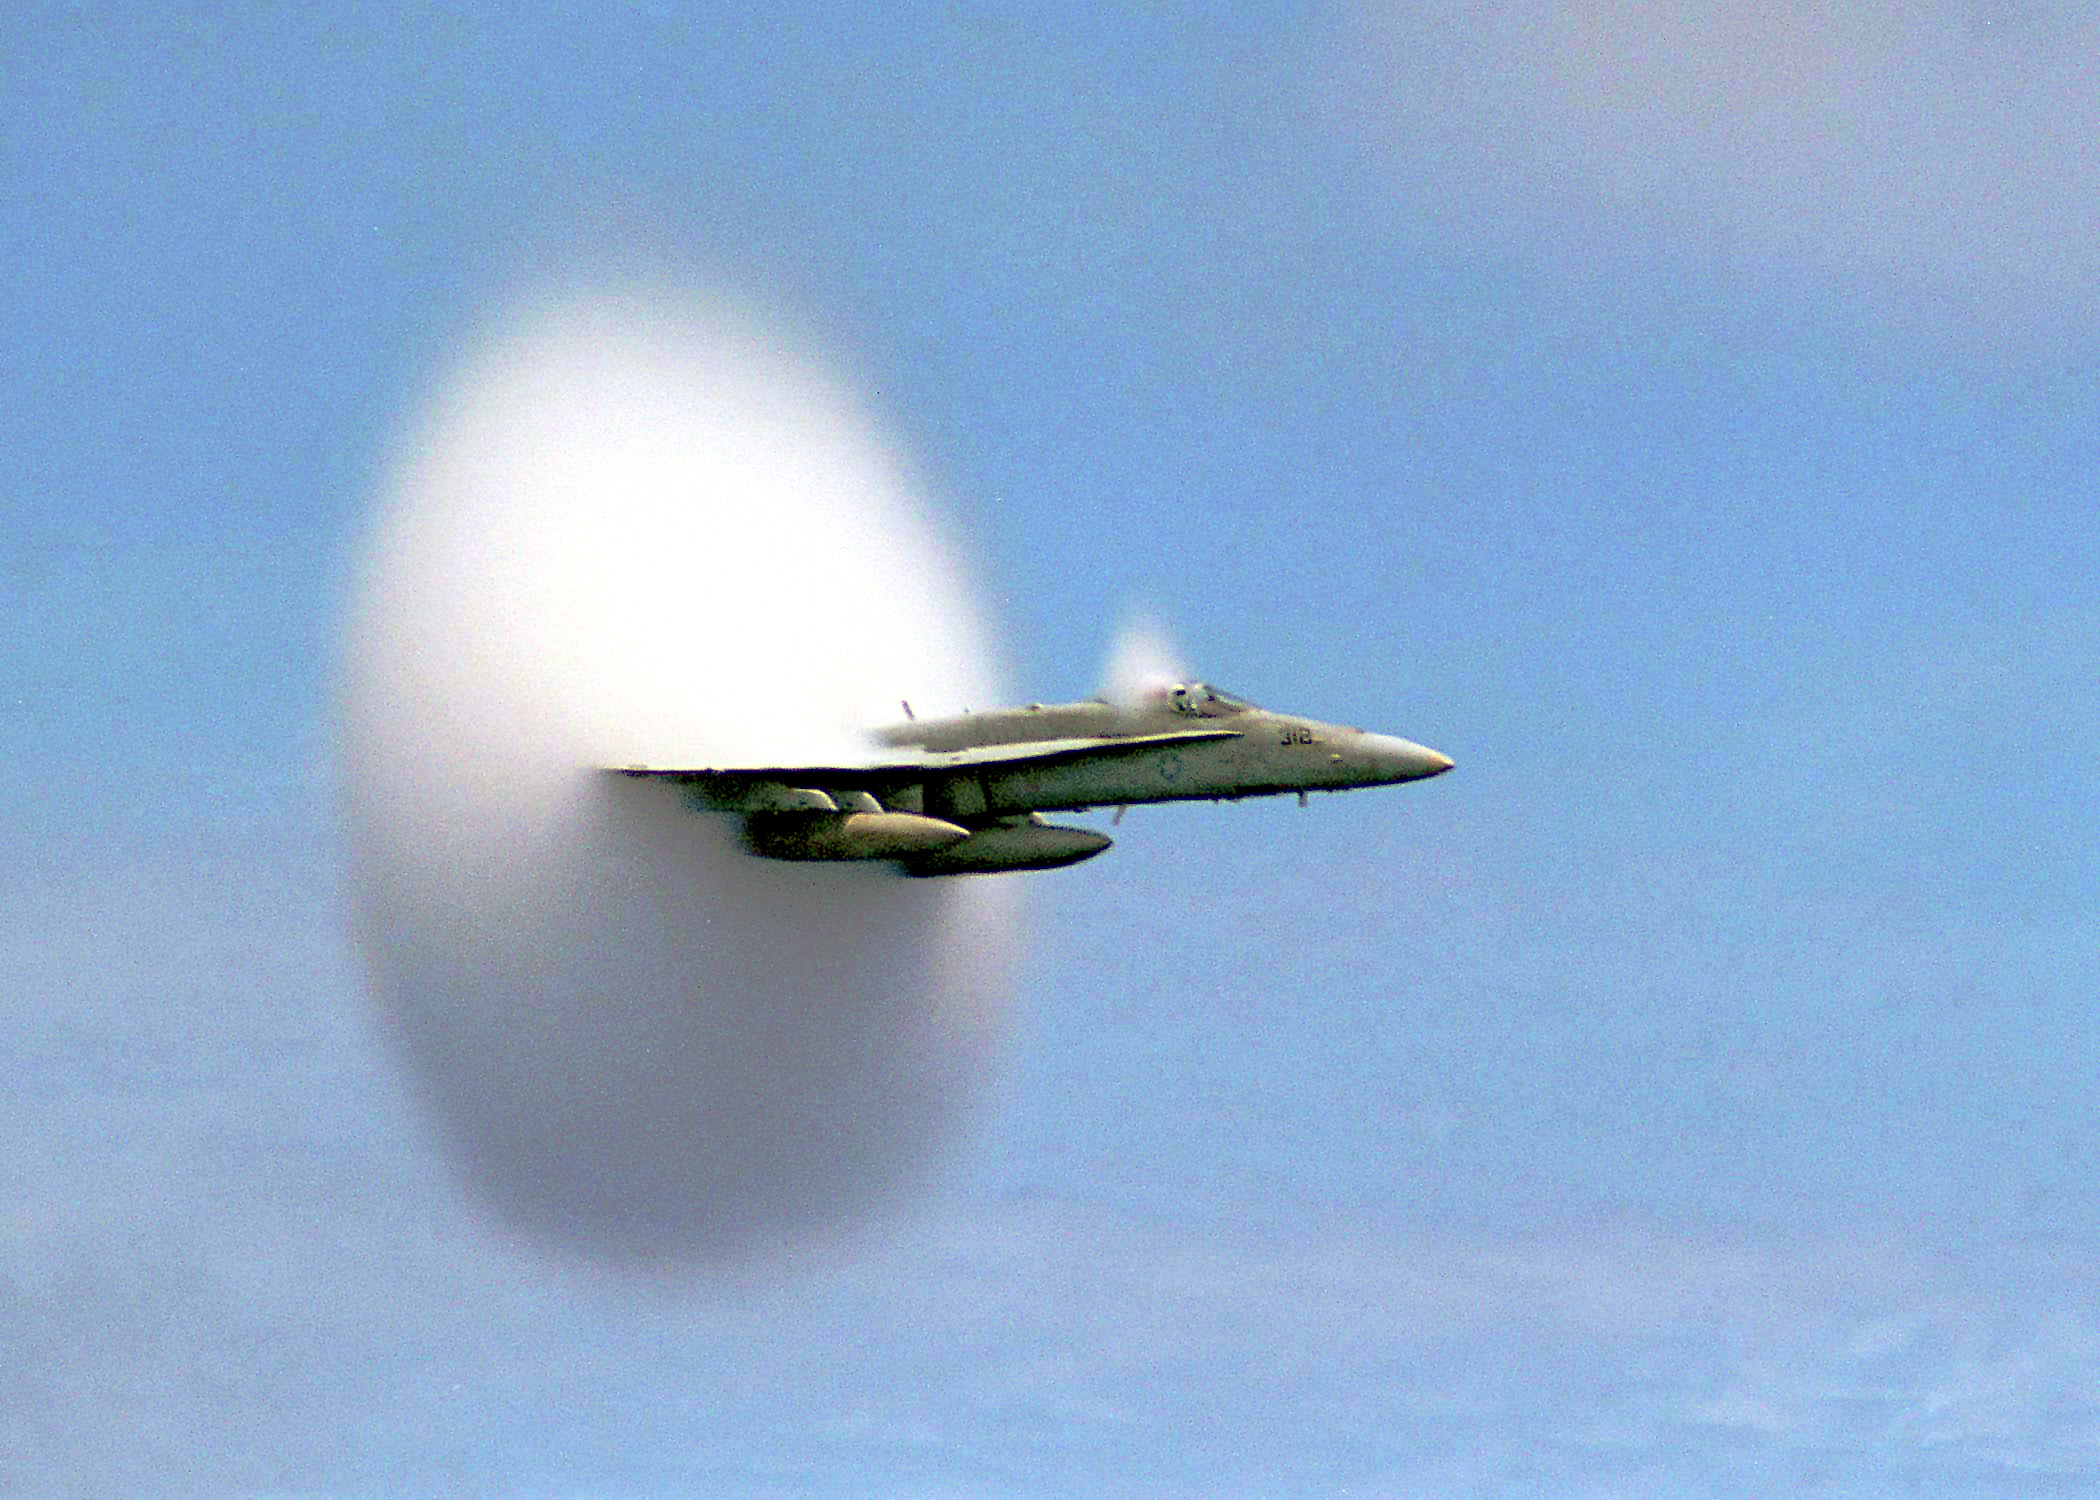
\includegraphics[height=8.0cm]{ambsthermopict/sightofsound.eps} 
} 
\caption{The shock wave of a supersonic airplane made visible
by condensation}
\label{breakingwave2} 
\end{figure}

\section{Mathematical Literature on Compressible Flow}
There is a vast literature on compressibe flow described by Euler's equations \cite{serre}, but basic questions about 
existence and wellposedness  of solutions are left without answers. The difficulty is that solutions of the Euler equations initiated from smooth initial data, which do exist as unique smooth solutions for some period of time,  develop shocks/turbulence and thus can continue only as non-smooth weak solutions with possible lack of physical meaning and uniqueness. 
To secure physical meaning entropy conditions of different forms are used, but it is now known which conditions will suffice to secure weak solutions to be physical. 

With sufficiently strong non-linear viscosities global existence of unique smooth solutions of Navier-Stokes equations can formally be proved by standard mathematical techniques, however without any assessment of wellposedness and physical meaning.  For constant viscosities results are lacking. The Navier-Stokes equations are thus as inaccessible to formal mathematical analysis as the Euler equations.

What remains is computation and we thus make a restart with RNS for Euler's equations and we do answer questions about existence and uniqueness related to wellposedness. 


One condition proposed in the literature is \emph{maximal dissipation of kinetic energy} \cite{dafermos}, but its is not clear that physics follows this principle. In RNS as best possible 
satisfaction of Euler's equations, it is rather a principle of minimal dissipation of kinetic energy as the smallest possible price to pay for non-smoothness. 


\small
\begin{quote}
A theory is the more impressive the greater the simplicity of its 
premises, the more different kinds of things it relates, and the more 
extended its area of applicability. Therefore the deep impression that 
classical thermodynamics made upon me. It is the only physical theory of 
universal content which I am convinced will never be overthrown, within 
the framework of applicability of its basic concepts.(Einstein)
\end{quote}
\begin{quote}
Nothing in life is certain except death, taxes and the second law of 
thermodynamics. All three are processes in which useful or accessible 
forms of some quantity, such as energy or money, are transformed into 
useless, inaccessible forms of the same quantity. That is not to say 
that these three processes don't have fringe benefits: taxes pay for 
roads and schools; the second law of thermodynamics drives cars, 
computers and metabolism; and death, at the very least, opens up 
tenured faculty positions. (Seth Lloyd, in \emph{Nature}, 2004)
\end{quote}
\normalsize 







\chapter{Viscosity Solutions to 1d Euler}

\small
\begin{quote} 
The total energy of the universe is constant; the total entropy is 
continually increasing. (Rudolf Clausius 1865)
\end{quote}
\begin{quote}
You believe in the God who plays dice, and I in complete
law and order in a world which objectively exists, and which I, in a wild
speculative way, am tryin to capture. Even the great initial success of 
Quantum Theory does not make me
believe in the fundamental dice-game, although I am well aware that younger
collegues interpret this as a consequence of senility. No doubt the 
day will come when we will see those instictive attitude was the correct one.
Some physicists. among them myself, cannot believe that we must abandon,
actually and forever, the idea of direct representation of physical reality
in space and time; or that we must accept then the view that events in nature
are analogous to a game of chance...In any case I am convinced that \emph{He} 
does not
throw dice. (Einstein)
\end{quote}
%\begin{quote} Everyone knows that heat can produce motion. That it possesses
%vast motive power no one can doubt, in these days when the steem engine is 
%everywhere so well known. The study of these enegines is of great interest,
%their importance is enormous, their use is contnually increasing, and they
%seem desined to produce a great revolution in the civilized world.
%(Carnot \cite{carnot} 1824).
%\end{quote}
%\begin{quote}...the whole procedure was an act of despair because a
%theoretical interpretation had to be found at any price, no matter
%how high that might be... (Planck on the statistical mechanics basis of 
%his radiation law)
%\end{quote}
%\begin{quote} Where does irreversibility come from? It does not come
%form Newton's laws. Obviously there must be some law, some
%obscure but fundamental equation. perhaps in electricty,
%maybe in neutrino physics, in which it \emph{does}
%matter which way time goes. (The Feynmman Lectures on Physics 1963)
%\end{quote}
%\begin{quote} The 2nd Law cannot be derived from purely mechanical
%laws. It carries the stamp of the essentially statitical nature of heat.
%(Bergman in Basic Theories of Physics 1951)
%\end{quote}













\normalsize

%We now proceed to formulate a deterministic form of the 2nd Law
%and then verify that RNS satisfies the 2nd Law. 
%For definiteness we may assume the gas to be perfect,
%but the 2nd Law will take the same form for a general state equation.

\section{Regularisation of Hamiltonian Systems}

We present in this chapter a short-cut to the  
computational foundation of thermodynamics in the setting of the Euler
equations in one space dimension (1d). 
In particular, we motivate a 2nd Law,
which we will below show to be satisfied by RNS in the full 3d case. 

We use the standard approach of \emph{viscous regularisation}
%but from a new perspective reflecting the fact that there are no 
%functions with  pointwise small (or zero) Euler 
%residuals. 
motivated by the fact that the Euler equations do not admit exact pointwise solutions, 
because of the inevitable appearance of turbulence/shocks. 
%In this perspective
%the precise form of the regularization becomes irrelevant, and we 
%can choose a regularization for which the existence of a 
%unique smooth regularized solution follows by standard analytical 
%mathematical techniques. 
We will view RNS solutions as specific regularised solutions, 
which are computed and thus exist and can be inspected.
We shall below in more detail investigate the precise form of
the regularisation in RNS, and discover that it has 
interesting features, not only from mathematical and computational,
but also from physical point of view. 

The basic idea in viscous regularisation of a Hamiltonian system
described by an equation $H(u)=0$ over a domain 
$\Omega\times [0,1]$ in space-time, such as the Euler equations, 
is to perturb the equation $H(u)=0$ into
\[
H(u_\nu )=\nu\Delta u_\nu \quad \mbox{in }\Omega\times [0,1],
\]
where $\nu >0$ is a small parameter representing a small (shear) viscosity,
and the Laplacian has a regularising or smoothing
effect on the solution.
 
The presence of the Laplacian (or possibly a higher order 
regularising differential operator such as the biLaplacian),
makes it possible in some cases to prove the existence of a 
pointwise solution $u_\nu$ to the regularised problem, 
a \emph{viscosity solution}, by standard techniques of mathematical 
analysis involving Sobolev and Gronwall inequalities, while  
the original Hamiltonian system is inaccessible to analysis
because the equation $H(u)=0$ lacks pointwise solutions.
For the regularised compressible Euler equations, technical
difficulties have hitherto prevented a full proof of existence of pointwise solutions.
But this is not crucial for the computational foundation 
since this is based on computed RNS-solutions with specific residual-based regularisation and not viscosity solutions, and
computed solutions do exist and can be inspected. 
We here use viscosity solutions to formally illustrate basic features of 
RNS-solutions such as the 2nd Law, which we then verify directly for 
RNS-solutions. 
%RNS delivers regularised approximate be viewed as specific 
%solutions, which are computed and thus do exist.  


If the regularised solution $u_\nu$ is \emph{smooth} in the sense that 
$\Delta u_\nu$
is of moderates size, then the perturbation $\nu\Delta u_\nu$ will be
small, because $\nu$ is small, and thus the regularised solution 
$u_\nu$ will be
an approximate pointwise solution of the Hamiltonian system 
with the Hamiltonian residual 
$H(u_\nu )$ being small in a pointwise sense. In this case the
the perturbation can be said to be \emph{regular}, and is inessential
in the sense that already the original problem has a pointwise solution
and regularisation is not needed. 
 
However, we consider problems where the Hamiltonian residual 
$H(u_\nu)$ is not small (in fact large) in regions with 
shocks/turbulence, 
while $H(u_\nu)$ remains small in a weak norm, so that
$\hat u_\nu$ still is an approximate solution
to the Hamiltonian system, but now only in a weak (but not pointwise)
sense.
The viscous term $\nu\Delta u$ will thus be pointwise large,
which is reflected by the fact that the total dissipation 
\[
D(u_\nu) =\int_\Omega \nu\vert\nabla u_\nu\vert^2dx
\]
is not small (of moderate size). In particular, the regularised 
solution $u_\nu$ is
\emph{non-smooth} in the sense that $\vert \nabla u_\nu\vert$ and
$\vert\Delta u_\nu\vert$ are locally
very large (of size $\nu^{-1}$ and $\nu^{-2}$ at shocks and of size 
$\nu^{-1/2}$ and $\nu^{-3/2}$
in turbulent regions, respectively). In this case the perturbation
is \emph{singular}, and is essential in the sense that
only the regularised problem has pointwise solutions. We thus
consider a Hamiltonian system with singular perturbation.

We understand that $D(u_\nu )$ results from multiplication
of  $-\nu\Delta u_\nu$ by $u_\nu$ and integration 
(by parts) over $\Omega$.
Typically, $D(u_\nu )$ will have a positive limit as $\nu$
tends to zero, which expresses an independence of the specific form of
the regularisation, that is the specific value of $\nu$, with 
always the term  $-\nu\Delta u_\nu$ balancing the non-zero 
Hamiltonian residual $H(u_\nu)$, with $\Delta u_\nu$ getting larger
as $\nu$ gets smaller. 

 
We will thus view the appearance of the regularisation term 
as a mathematical formality and we do not seek to connect it to
any physical ``shear viscosity''. This is because the appearance of 
``shear viscosity'' in Hamiltonian systems  without viscosity, such 
as the Euler equations,  represents the main mystery of the classical 
2nd Law. We thus do not accept the common argument that ``there is always some form
of (shear) viscosity, which we can model by a Laplacian''.
The key question is from where such a viscosity comes in a inviscid
flow.  

We shall see that RNS offers a new answer  to this key 
question, where the residual regularisation appears as a 
loss of kinetic energy because the momentum equation cannot
be satisfied pointwise, and not as any form of classical
(shear) viscosity. The loss of kinetic energy (which is transformed
into heat energy) can be viewed as a ``fine'' to be paid 
because the law $H(u)=0$ is heavily violated pointwise. 
The fine can take many forms, since there are many possible
forms of regularisation, while the violation essentially remains the same.
We shall see that RNS penalises a large residual $H(\hat u)$, 
while classical viscous regularisation penalises all large derivates, 
not only the particular combination of the residual. 

RNS thus
has ``fine-tuned'' penalisation with the fine being as close as possible 
to the violation, like a penicillin with narrow spectrum killing
only microbes producing the symptom, which suggests that
RNS can be given a physical significance. On the ohter hand,
classical viscous regularisation, is more like a broad band penicillin 
killing both microbes and healthy bacteria, 
and its physical significance has remained a mystery. 


To sum up, we start from a Hamiltonian system without
pointwise solutions (the Euler equations), 
which we replace by a regularised system
with pointwise solutions (by viscous regularisation or RNS), 
which can be viewed as approximate solutions
to the original system. We find that certain mean-values of 
the regularised solutions 
show little dependence on the specific
form of the regularisation (the viscosity or the mesh size), 
and thus can be viewed as stable outputs
of approximate solutions to the original system.
We first carry out the argument for viscous regularisation 
and then return below to the real case of RNS regularisation.



 
%We recall that it is coomon in mathematical analysis 
%of ``viscosity solutions'' of Hamilton-Jacobi equations
%Thus, simply adding viscosity to a Hamiltonian system does not
%explain anything, unless the nature of the viscosity is explained,
%and this is the main mystery. This remark in particular 
%relates to the mathematics of Hamiltonian systems or Hamilton-Jacobi
%equations, for which the concept of ``viscosity solution'' 
%has played an important role, but again the rationale of 
%simply adding viscosity has remained unclear. 
%In contrast, RNS includes a certain form
%of viscosity, a certain finite precision computational viscosity,
%which appears because the Euler equations do not
%have infinite precision exact solutions, due to 
%turbulence/shocks, but only finite precision approximate RNS
%solutions with a certain weighted least squares residual control
%acting like a viscosity. 

%We thus rationalize the appearance
%of ``viscositgy'' in turbulent Euler solutions, as a consequence
%of the non-existence of exact solutions, or as a necessary fine to pay 
%because the conservation laws cannot be satisfied exactly. Thus RNS
%does the ``best possible'' out an impossible situation, and
%the best possible involves a certain form of viscosity. 
%The appearance of  viscous effects in RNS thus may be viewed to follow
%from a Leibnizian Best of Worlds principle, which gives
%the 2nd Law a rational basis: The 2nd Law is a consequence
%of optimality of a Best of Worlds.     
  


\section{1d Euler}
 
We consider an inviscid perfect gas 
enclosed in a tube represented by the interval $\Omega =(0,1)$ in space
over a time interval $I=(0,1]$ and we assume
that $f=0$ and $g=0$. The 1d Euler equations
expressing the 1st Law as conservation of mass, momentum and 
internal energy, formally take the form: 
Find $\hat u\equiv (\rho ,m,e)$ such that
with $v^\prime =\frac{\partial v}{\partial x}$
\begin{equation}\label{euler1d1}
\begin{array}{rcl}
R_\rho (\hat u)\equiv\dot \rho +(\rho u )^\prime &=&  0 \quad \mbox{in } Q, \\
R_m(\hat u)\equiv\dot m +(mu +p)^\prime &=&  0 \quad \mbox{in } Q, \\
R_e(\hat u)\equiv\dot e +(e u )^\prime +pu^\prime &=&  0 \quad \mbox{in } Q, \\
u(0,t)=u(1,t)&=&0\quad  t\in I,\\
\hat u(\cdot ,0)&=&\hat u^0\quad \mbox{in } \Omega , 
\end{array} 
\end{equation}
where  
$p=\gamma e$ with $\gamma >0$ and $u=\frac{m}{\rho}$, or in short form
\begin{equation}\label{euler1d2}
\begin{array}{rcl}
R(\hat u)&=&  0 \quad \mbox{in } Q, \\
u(0,t)=u(1,t)&=&0\quad  t\in I,\\
\hat u(\cdot ,0)&=&\hat u^0\quad \mbox{in } \Omega , 
\end{array} 
\end{equation} 
where $R=(R_\rho ,R_m,R_e)$. 
%Find $(\rho ,m,\epsilon )$ 
%depending on $(x,t)\in Q\equiv J\times I\equiv [0,1]\times [0,1]$ such that
%\begin{equation}\label{euler1d}
%\begin{array}{rcl}
%\dot \rho +(\rho u )^\prime&=&  0 \quad \mbox{in } Q, \\
%\dot m +(mu +p)^\prime &=&  0 \quad \mbox{in } Q, \\
%\dot \epsilon +(\epsilon u +pu)^\prime&=&  0 \quad \mbox{in } Q, \\
%u(0,t)=u(1,t)&=&0\quad  t\in I,\\
%\hat u(\cdot ,0)&=&\hat u^0\quad \mbox{in } \Omega , 
%\end{array} 
%\end{equation}
%where the total energy
%$\epsilon =k +e$ is the sum of the kinetic energy $k =\rho u^2/2$ and 
%internal heat energy $e=\rho T$, $u=\frac{m}{\rho} $, 
%$p=(\gamma -1)\rho T$ and $\gamma >1$. For a mono-atomic gas $\gamma =5/3$.
%Further, $v^\prime =\frac{\partial v}{\partial x}$. 

%Strictly speaking, the 1st Law in classical form expresses conservation
%of total energy, while conservation of momentum corresponds to Newton's
%second law and conservation of mass reflects that mass cannot be destroyed.
%However, it is convenient to let the 1st Law express conservation of
%both mass, momentum and total energy, so that in short the 
%Euler equations (formally) express the 1st Law.

%We will replace the equation for the total energy
%$\epsilon$ by the following equation for the internal 
%energy $e$:
%\begin{equation}\label{conservatione}
%\dot e +(eu)^\prime +pu^\prime =  0  \quad \mbox{in } Q, 
%\end{equation}
%which follows by multiplication of the momentum equation by $u$ and subtraction
%from the equation for $\epsilon$, and using also the equation for $\rho$ in the
%form $(\dot\rho +(\rho u)^\prime )\frac{u^2}{2}=0$. 





%For simplicity, we choose $\gamma =2$ in which case
%the state equation takes the form $p=\bar\gamma \rho T$, where $T$ is the temperature
%measuring the internal energy, and we also have $e=\rho\frac{w^2}{2}+\rho T
%=\rho\frac{w^2}{2}+\bar\gamma p$.
 
\section{Formal Reversiblity}

The Euler equations (\ref{euler1d1}) without regularization
are formally \emph{reversible}:
Changing the sign of the velocity $u$ and the direction of time (the
sign of the time-derivative $\dot u$), the Euler equations obviously
remain unchanged. This means that if $\hat u(t)$ is a solution to the
Euler equations in forward time 
on $[0,T]$ taking the initial value $\hat u(0)$ to 
the final value $\hat u(T)$, we
obtain a solution in backward time taking $\hat u(T)$ back to
$\hat u(0)$ by reversing the velocity at time $\bar t$. Of course
we can view this solution as proceeding in forward time by just
continuing counting time forward after the velocity reversal.

We conclude that if the Euler equations 
have a pointwise solution then it can be 
turned into a perpetuum mobile running for ever without 
consuming any energy, for ever bouncing
back and forth by repeated reversal of the velocity at two given
time instances.

\section{Factual Irreversibility}
The trouble with the above argument is that
the Euler equations lack pointwise solutions and thus
the implication is empty. In contrast viscosity solutions
to the regularized Euler equations exist, but these solutions
are turbulent with substantial turbulent dissipation 
and thus are irreversible. Therefore a perpetuum mobile is
impossible.

We sum up: The exact solutions which would have been reversible if they
had existed, do not exist. The viscosity solutions which do exist, 
are not reversible. This is the main lesson of this book, and resolves the 
main open problem of classical thermodynamics: \emph{Loschmidt's paradox}
asking how irreversibility can arise in a reversible system.

\section{Energy Estimates for Viscosity Solutions}


We shall now prove that a viscosity solutions 
of the regularized 1d Euler equations 
(\ref{euler1d1}) is a \emph{dissipative weak solution} of the Euler
equations in the sense that its Euler residual 
is small in a weak sense and it satisfies a 2nd Law 
expressing an irreversible transfer
from kinetic to heat energy in the form of turbulent/shock dissipation.
In short we prove that viscosity solutions are dissipative weak
solutions of the Euler equations.

We thus consider the following 
regularized version
of (\ref{euler1d1}): Find $\hat u_{\nu ,\mu}\equiv\hat u=(\rho ,m,e)$ such that

\begin{equation}\label{euler1dreg}
\begin{array}{rcl}
\dot \rho +(\rho u )^\prime&=&  0 \quad \mbox{in } Q, \\
\dot m +(mu +p)^\prime &=&(\nu u^{\prime})^\prime +(\mu pu^\prime )^\prime \quad \mbox{in } Q, \\
\dot e +(eu)^\prime +pu^\prime &=&  \nu (u')^2 \quad \mbox{in } Q, \\
u(0,t)=u(1,t)&=&0\quad  t\in I,\\
\hat u(\cdot ,0)&=&\hat u^0\quad \mbox{in } \Omega , 
\end{array} 
\end{equation}
where $p=\gamma e$, and 
$\nu >0$ and $\mu\ge 0$ are small parameters with $\nu$ representing
\emph{shear viscosity} and $\mu$ a form of \emph{bulk viscosity}
with $\mu =0$ if $u^\prime <0$. For
simplicity, we here suppress the subindices $\nu$ and  $\mu$. We here
use the balance equation for the internal energy $e$,  modified
to account for the contribution to the internal energy from 
shear viscosity, but without contribution from bulk viscosity,
which we consider as a penalty.
We observe that only the velocity $u$ 
is subject to regularization, which gives (as we will see below) 
the momentum equation
a different quality than the balance equations for 
mass and internal energy, both involving $u$ as a coefficient.

We shall see that it is natural to choose the regularization parameter
$\nu$ much smaller than $\mu$, and thus the main effect of the regularization
comes from the bulk viscosity $\mu$, rather than from
the usual shear viscosity $\nu$. We shall see that the bulk
viscosity prevents fluid particles from colliding, or more precisely,
prevents faster fluid particles to overtake slower particles
(along the same streamline), which thus is the main effect of the 
regularization and not shear viscosity.
  

%Existence and uniqueness of a pointwise solution 
%$\hat u_{\nu ,\mu}$ to the regularized
%problem follows by standard analytical mathematical techniques.
%The regularization of the momentum equation ensures that the velocity
%$u$ is differentiable, from which follows that also $\rho$ and $e$ are 
%differentiable, and thus the equations of (\ref{euler1dreg})
%are satisfied pointwise.



We shall now prove that $\hat u=\hat u_{\nu ,\mu}$ satisfies
\begin{equation}\label{euler1dweak}
\Vert R_m(\hat u)\Vert_{-1}\le 
\frac{\sqrt{\nu}}{\sqrt{\mu}}+\sqrt{\mu},
\end{equation}
where $\Vert\cdot\Vert_{-1}$ denotes the $L_2(I;H^{-1}(J))$-norm,
while obviously $R_\rho (\hat u)=0$ and $R_e(\hat u)\ge$ in a pointwise sense
in $\Omega\times I$. 
Further, we shall observe that $\hat u$ satisfies the following 
2nd Law:
\[
\dot K \le W-D,\quad \dot E =-W+D,
\]
where 
\[
K=\int_Jkdx,\quad E=\int_Jedx, \quad W=\int_Jpu^\prime dx, 
\quad D =\int_J \nu (u^\prime )^2\, dx>0.
\]

Choosing $\mu =\epsilon$ and $\nu =\epsilon^2$, we can assure that
$\Vert R_m(\hat u_{\nu ,\mu})\Vert_{-1}\le 2\sqrt{\epsilon}$ for 
any positive $\epsilon$.
We shall prove the following result on the existence
of \emph{dissipative weak approximate solutions} to the 1d Euler equations:

\begin{theorem}\label{exist1d} 
A viscosity solution $\hat u$ of the regularized
Euler equations (\ref{euler1d1}) satisfies 
\[
R_\rho (\hat u)=0\quad \mbox{in }\Omega\times I,\quad \Vert R_m(\hat u)\Vert_{-1}\le TOL,\quad R_e(\hat u)\ge 0\quad\mbox{in }\Omega\times I ,
\]
where $TOL=\frac{\sqrt{\nu}}{\sqrt{\mu}}+\sqrt{\mu}$,
together with the 2nd Law
\begin{equation}\label{2ndlaw1d}
\dot K \le W-D,\quad \dot E =-W+D, \quad D>0.
\end{equation}
\end{theorem}

We understand that Theorem \ref{exist1d} states certain 
properties of the regularised solution $u_{\nu ,\mu}$ 
in terms of its Euler residuals, without
explicitly referring to the regularisation,    
where the 2nd Law compensates for the 
fact that the momentum residual $R_m(\hat u)$ is only
required to be small in a weak norm, and $R_e(\hat u)$ is allowed
to be pointwise positive. We note that by the 2nd Law (\ref{2ndlaw1d})
it follows that
\begin{equation}\label{1stlaw}
\dot K+\dot E\le 0
\end{equation}
stating that the 
integral (or totality) in space of the total energy $\epsilon$ 
cannot increase. 
%We shall see below that an RNS solution is a
%dissipative weak solution. 

To make the notion of dissipative weak
solution really useful, we have to connect it to 
\emph{output uniqueness}. We will return to this basic aspect
below in the context of RNS, using directly the properties of RNS
without passing through Theorem \ref{exist1d}. We can thus view
Theorem \ref{exist1d} as a connection to a classical
analytical technique of regularized solutions, which we will not
pursue in detail, because what we can compute are RNS solutions,
not classical regularized solutions, and because a RNS solution can be viewed
as a (new) form of  
regularized solution.   

Since the concept of weak solution can be viewed as expressing 
a form of approximate solution, with an exact solution 
being a (strong) pointwise solution, we can condense the notation to 
\emph{dissipative weak solution}. In short, we will thus
prove the existence of dissipative weak solutions to the Euler
equations and below see that a RNS solution is a dissipative
weak solution.

\medskip
\noindent 
{\bf Proof of Theorem \ref{exist1d}}: 
The basic technical step is to multiply the momentum equation
by $u$, omitting for simplicity the indices $\nu$ and $\mu$,
and use the mass balance equation in the form
$\frac{u^2}{2}(\dot \rho +(\rho u)^\prime )=0$, to get
\begin{equation}\label{k1}
\dot k +(ku)^\prime +p^\prime u -\mu (pu^\prime )^\prime u-\nu u^{\prime\prime}u =0.
\end{equation}
By integration in space it follows that $\dot K\le W-D$,
and similarly it follows that $\dot E =-W+D$ from the 
equation for $e$, which proves the 2nd Law.
Adding next (\ref{k1}) to the equation for the internal energy $e$ and
integrating in space, gives
\[
\dot K+\dot E +\int_0^1 \mu p(u^\prime )^2\, dx =0,
\]
since
\[
\int_0^1 (p^\prime u + pu^\prime)dx = \int_0^1(pu)^\prime dx =0,
\] 
and thus after integration in time
\begin{equation}\label{energy1}
K(1)+E(1) +\int_Q \mu p(u^\prime )^2\, dxdt =K(0)+E(0).
\end{equation}

We now need to show that $E(1)\ge 0$ (or more generally that $E(t)>0$
for $t\in I$), and to this end we
rewrite the equation for the internal energy as follows:
\[
\frac{De}{Dt} +(\gamma +1) eu^\prime =  \nu (u')^2,
\]
where $\frac{De}{Dt}=\dot e+ue^\prime$ is the material derivative
of $e$ following the fluid particles with velocity $u$.
 Assuming that $e(x,0)> 0$ for
$0\le x\le 1$, it follows
that $e(x,1)>0$ for $0\le x\le 1$, and thus $E(1)>0$.
Assuming $K(0)+E(0)=1$ the energy estimate 
(\ref{energy1}) thus shows that
\begin{equation}\label{mupu1}
\int_Q\mu p(u^\prime )^2\, dxdt \le 1,
\end{equation}
and also that $E(t)\le 1$ for $t\in I$.

Next, integrating (\ref{k1}) in space and time gives
\[
K(1)+\int_Q\nu (u^\prime )^2dxdt=\int_Q pu^\prime dxdt -
\int_Q\mu p(u^\prime )^2dxdt \le \frac{1}{\mu}\int_Qpdxdt\le \frac{1}{\mu},
\]
where we used that $\int_Q p dxdt=\gamma \int_Qedxdt \le \int_IE(t)dt\le 1$. It follows that
\begin{equation}\label{nuu21}
\int_Q\nu (u^\prime )^2dxdt\le \frac{1}{\mu}.
\end{equation}
By standard estimation it follows from (\ref{mupu1}) and (\ref{nuu21}) that
\[
\Vert R_m(\hat u)\Vert_{-1}\le \sqrt{\mu}+\frac{\sqrt{\nu}}{\sqrt{\mu}},
\]
and the proof can be completed in an obvious fashion.

\section{Irreversibility by the 2nd Law}

The 2nd Law (\ref{2ndlaw1d}) 
states an irreversible
transfer of kinetic energy to heat energy for in the presence of shocks 
with $D >0$, which is the generic case. 
On the other hand, the sign of $W$ is variable and
thus the corresponding energy transfer may go in either direction. 



\section{Compression and Expansion}

The 2nd Law (\ref{2ndlaw1d}) states that there is a transfer
of kinetic energy to heat energy if $W<0$, that is under compression
with $u'<0$, and a transfer from heat to kinetic energy 
if $W>0$, that is under expansion with $u'>0$. As we just remarked, 
there is a transfer from kinetic to heat energy for solutions
with shocks with $D > 0$. 


Returning to Joule's experiment, we see by the 2nd Law that contraction back
to the original volume from the final rest state in the double volume,
is impossible, because the only way the gas can be set into motion is 
by expansion.



 

%\section{On the Nature of Regularization}
%Not shear, but expansion.

\chapter{Viscosity Solutions to 3d Euler}

\small
%\begin{quote} 
%The total energy of the universe is constant; the total entropy is 
%continually increasing. (Rudolf Clausius 1865)
%\end{quote}
\begin{quote} Everyone knows that heat can produce motion. That it possesses
vast motive power no one can doubt, in these days when the steam engine is 
everywhere so well known. The study of these engines is of great interest,
their importance is enormous, their use is continually increasing, and they
seem desined to produce a great revolution in the civilised world.
(Carnot \cite{carnot} 1824).
\end{quote}
\begin{quote} But maybe that is our mistake: 
maybe there are no particle positions and velocities, but only waves. 
It is just that we try to fit the waves to our preconceived ideas of 
positions and velocities. The resulting mismatch is the cause of the 
apparent unpredictability.(Stephen Hawking)
\end{quote}
\begin{quote}
What  wanted to say was just this: In the present
circumstances the only profession I would choose would be one where
earning a living had nothing to do with the search for knowledge.
(Einstein's last letter to Born Jan 17 1955 shortly before his death on 
the 18th of April, 
probably referring to Born's  statistical interpretation 
of quantum mechanics).
\end{quote} 

%\begin{quote}...the whole procedure was an act of despair because a
%theoretical interpretation had to be found at any price, no matter
%how high that might be... (Planck on the statistical mechanics basis of 
%his radiation law)
%\end{quote}
%\begin{quote} Where does irreversibility come from? It does not come
%form Newton's laws. Obviously there must be some law, some
%obscure but fundamental equation. perhaps in electricty,
%maybe in neutrino physics, in which it \emph{does}
%matter which way time goes. (The Feynmman Lectures on Physics 1963)
%\end{quote}
%\begin{quote} The 2nd Law cannot be derived from purely mechanical
%laws. It carries the stamp of the essentially statitical nature of heat.
%(Bergman in Basic Theories of Physics 1951)
%\end{quote}













\normalsize

  


\section{3d Euler}

We now show that the above result for the 1d Euler equations
directly extends to 3d.
We thus consider the 3d Euler equations for an inviscid perfect gas 
enclosed in a volume $\Omega$ in $\bbR^3$ with boundary $\Gamma$
over a time interval $I=(0,1]$, assuming as above that the 
applied force $f=0$: 
Find $\hat u=(\rho ,m,e)$ 
depending on $(x,t)\in Q\equiv \Omega\times I$ such that
\begin{equation}\label{euler3d1}
\begin{array}{rcl}
R_\rho (\hat u)\equiv\dot \rho +\nabla\cdot (\rho u )&=&  0 \quad \mbox{in } Q, \\
R_m(\hat u)\equiv\dot m +\nabla\cdot (mu) +\nabla p&=&  0 \quad \mbox{in } Q, \\
R_e(\hat u)\equiv\dot e +\nabla\cdot (eu)+p\nabla\cdot u &=& 0  \quad \mbox{in } Q,\\ 
u\cdot n&=&0\quad \mbox{on } \Gamma\times I\\
\hat u(\cdot ,0)&=&\hat u^0\quad \mbox{in } \Omega , 
\end{array} 
\end{equation}
where $u=\frac{m}{\rho}$ and 
$p=\gamma e$ with $\gamma >0$. 




\section{Energy Estimates for Viscosity Solutions}


We consider the following regularized version
of (\ref{euler3d1}): Find $\hat u_{\nu ,\mu}\equiv\hat u=(\rho ,m,e)$ such that

\begin{equation}\label{euler3dreg}
\begin{array}{rcl}
R_\rho (\hat u)&=&  0 \quad \mbox{in } Q, \\
R_m (\hat u)&=&\nabla\cdot (\nu\nabla u) +
\nabla (\mu p\nabla\cdot u) \quad \mbox{in } Q, \\
R_e (\hat u) &=&  \nu \vert\nabla u\vert^2 \quad \mbox{in } Q, \\
u &=&0\quad  \quad\mbox{on } \Gamma\times I,\\
\hat u(\cdot ,0)&=&\hat u^0\quad \mbox{in } \Omega , 
\end{array} 
\end{equation}
where $\nu >0$ is a  shear viscocity and $\mu\ge 0$ 
a bulk viscosity with $\mu =0$ if $\nabla\cdot u <0$, and 
$\vert\nabla u\vert^2 =\sum_{i=1}^3\vert\nabla u_i\vert^2$. 

As already indicated, the existence of a pointwise solution 
$\hat u_{\nu ,\mu}$ to the regularised
problem is an open problem of mathematical analysis.
However, we only use the regularised problem to formally illustrate basic
properties of RNS-solutions, which we prove directly below.


%We choose in (\ref{euler3dreg}) a 4th order regularization for convenience.
%It is also possible to use 2nd order regularization replacing
%$\Delta (\nu\Delta u)$ by $\nabla\cdot (\nu\nabla u)$ with
%a slight dependence of $\nu$ on $\vert\nabla u\vert$. In RNS
%the regularization mainly results from the least squares stabilization
%which introduces forms of both shear and bulk viscosity 
%with emphasis on the latter. RNS also contains a
%shock-capturing viscosity of the form $\nabla\cdot (\nu\nabla u)$
%with $\nu$ depending on Euler residuals, which is active
%only at shocks and there eliminates unphysical (small) oscillations.

We shall now prove that $\hat u=\hat u_{\nu ,\mu}$ satisfies
\begin{equation}\label{euler1dweak}
\Vert R_m(\hat u)\Vert_{-1}\le 
\frac{\sqrt{\nu}}{\sqrt{\mu}}+\sqrt{\mu},
\end{equation}
where $\Vert\cdot\Vert_{-1}$ denotes the $L_2(I;H^{-1}(\Omega ))$-norm,
while we may assume that $R_\rho (\hat u)=0$ and $R_e(\hat u)\ge 0$ in a pointwise sense
in $Q$. We shall also find that $\hat u$ satisfies the following 
2nd Law:
\[
\dot K \le W-D,\quad \dot E =-W+D,
\]
where 
\[
K=\int_\Omega k\, dx,\quad E=\int_\Omega e\, dx, \quad W
=\int_\Omega p\nabla\cdot u\, dx, 
\quad D =\int_\Omega \nu \vert\nabla u\vert^2\, dx.
\]

Choosing $\mu =\epsilon$ and $\nu =\epsilon^2$, we can assure that
$\Vert R_m(\hat u_{\nu ,\mu})\Vert_{-1}\le TOL$ for 
any positive tolerance $TOL$.
We shall thus show the following formal result on the existence
of \emph{dissipative weak approximate solutions} to the 3d Euler equations:

\begin{theorem}\label{exist3d} 
A viscosity solution $\hat u$ of the regularized
Euler equations (\ref{euler3d1}) satisfies 
\[
R_\rho (\hat u)=0\quad \mbox{in }\Omega\times I,\quad 
\Vert R_m(\hat u)\Vert_{-1}\le TOL,\quad R_e(\hat u)\ge 0\quad\mbox{in }\Omega\times I ,
\]
where $TOL =\frac{\sqrt{\nu}}{\sqrt{\mu}}+\sqrt{\mu}$,
together with the 2nd Law
\begin{equation}\label{2ndlaw3d}
\dot K \le W-D,\quad \dot E =-W+D, \quad D>0.
\end{equation}
\end{theorem}

As above, we note that Theorem \ref{exist1d} states certain 
properties of the regularized solution $u_{\nu ,\mu}$ 
in terms of its Euler residuals, without
explicitely referring to the regularization,    
where the 2nd Law compensates for the 
fact that the momentum residual $R_m(\hat u)$ is only
required to be small in a weak norm, and $R_e(\hat u)$ is allowed
to be pointwise positive. We note that by the 2nd Law it follows
that
\begin{equation}\label{1stlaw}
\dot K+\dot E\le 0
\end{equation}
stating that the 
integral (or totality) in space of the total energy $\epsilon$ 
cannot increase. We shall see below that a RNS solution is a
dissipative weak approximate solution. 
%In this setting
%the norm $\Vert\cdot\Vert_{-2}$ is replaced by 
%$\Vert\cdot\Vert_{-1}$ in conformity with the 1d case. 

%To make the notion of dissipative weak
%approximate solution really useful, we have to connect it to 
%\emph{output uniqueness}. We will return to this basic aspect
%below in the context of RNS, using directly the properties of RNS
%without passing through Theorem \ref{exist3d}. We can thus view
%Theorem \ref{exist3d} as a connection to a classical
%analytical technique of regularized solutions, which we will not
%pursue in detail, because what we can compute are RNS solutions,
%not classical regularized solutions, and because a RNS solution can be viewed
%as a (different new) form of  regularized solution.   


\medskip
\noindent 
{\bf Proof of Theorem \ref{exist3d}}: 
The basic technical step is to multiply the momentum equation
by $u$, and use the mass balance equation in the form
$\frac{\vert u\vert^2}{2}(\dot \rho +\nabla\cdot (\rho u)=0$, to get
\begin{equation}\label{k}
\dot k +\nabla\cdot (ku)+\nabla p\cdot u -\nabla (\mu p\nabla\cdot u)\cdot u+ 
\nabla\cdot (\nu \nabla u)\cdot u =0.
\end{equation}
By integration in space it follows that $\dot K\le W-D$,
and similarly it follows that $\dot E =-W+D$ from the 
equation for $e$, which proves the 2nd Law.
Adding next (\ref{k}) to the equation for the internal energy $e$ and
integrating in space, gives
\[
\dot K+\dot E +\int_\Omega \mu p(\nabla\cdot u)^2\, dx =0,
\]
since
\[
\int_\Omega (\nabla p\cdot u + p\nabla\cdot u)dx = \int_\Omega \nabla\cdot (pu) dx =0,
\] 
and thus after integration in time
\begin{equation}\label{energy1}
K(1)+E(1) +\int_Q \mu p(\nabla\cdot u)^2\, dxdt =K(0)+E(0).
\end{equation}

We now need to show that $E(1)\ge 0$ (or more generally that $E(t)>0$
for $t\in I$), and to this end we
rewrite the equation for the internal energy as follows:
\[
\frac{De}{Dt} +(\gamma +1) e\nabla\cdot u=  \nu \vert\nabla u\vert^2,
\]
where $\frac{De}{Dt}=\dot e+u\cdot\nabla e$ is the material derivative
of $e$ following the fluid particles with velocity $u$.
 Assuming that $e(x,0)> 0$ for
$x\in\Omega $, it follows
that $e(x,1)>0$ for $x\in\Omega$, and thus $E(1)>0$.
Assuming $K(0)+E(0)=1$ the energy estimate 
(\ref{energy1}) thus shows that
\begin{equation}\label{mupu}
\int_Q\mu p(\nabla\cdot u )^2\, dxdt \le 1,
\end{equation}
and also that $E(t)\le 1$ for $t\in I$.

Next, integrating (\ref{k}) in space and time gives
\[
K(1)+\int_Q\nu\vert\nabla u\vert^2dxdt=\int_Q p\nabla\cdot udxdt -
\int_Q\mu p(\nabla\cdot u)^2dxdt \le \frac{1}{\mu}\int_Qpdxdt\le \frac{1}{\mu},
\]
where we used that $\int_Q p dxdt=\gamma \int_Qedxdt \le \int_IE(t)dt\le 1$. It follows that
\begin{equation}\label{nuu2}
\int_Q\nu\vert\nabla u\vert^2dxdt\le \frac{1}{\mu}.
\end{equation}
By standard estimation it follows from (\ref{mupu}) and (\ref{nuu2}) that
\[
\Vert R_m(\hat u)\Vert_{-1}\le \sqrt{\mu}+\frac{\sqrt{\nu}}{\sqrt{\mu}},
\]
and the proof can be completed in an obvious fashion.

\section{Irreversibility by the 2nd Law}

The 2nd Law (\ref{2ndlaw3d}) states an irreversible
transfer of kinetic energy to heat energy in the presence of  
shocks/turbulence with $D >0$, which is the generic case. 
On the other hand, the sign of $W$ is variable and
thus the corresponding energy transfer may go in either direction. 



\section{Compression and Expansion}

The 2nd Law (\ref{2ndlaw3d}) states that there is a transfer
of kinetic energy to heat energy if $W<0$, that is under compression
with $\nabla\cdot u<0$, and a transfer from heat to kinetic energy 
if $W>0$, that is under expansion with $\nabla\cdot u>0$. 

Returning to Joule's experiment, we see by the 2nd Law that contraction back
to the original volume from the final rest state in the double volume,
is impossible, because the only way the gas can be set into motion is 
by expansion.



 

\section{A 2nd Law witout Entropy}

We note that the 2nd Law (\ref{2ndlaw3d}) is expressed in terms of 
the kinetic energy $K$, the heat energy $E$ and the work $W$,
and does not involve any concept of entropy $S$. This relieves us from
the task of finding a physical significance of $S$ and 
a physical justification of a classical 2nd Law of the form $dS\ge 0$.
We thus circumvent the main difficulty of classical thermodynamics
based on statistical mechanics, while we reach the same goal 
as statistical mechanics
of explaining irreversibility in formally reversible Newtonian mechanics.

Note that since the new 2nd Law is a consequence of the 1st Law and
RNS computation, we can ``forget" the 2nd Law: It is automatically
satisfied without special attention. This is like ``forgetting"
to keep the balance while walking, because is automatically
maintained without conscious attention. 






\iffalse  % --- removed in shortened layout: redundant 2nd-Law revisit + redundant RNS chapter (kept single canonical RNS chapter below) ---
\chapter{Classical vs New 2nd Law}

\small
%\begin{quote} Thermodynamics is a funny subject. The first time you go through
%it, you don't understand it at all. The second time you go through it,
%you think you understand except a few small points. The third time you go
%through it, you know that you don't understand it, but by that time you are
%so used to it, that it doesn't bother you any more. (Sommerfeld).
%\end{quote}


\begin{quote}
It seems to me that the concept of probability
is terribly mishandled these days. A probabilistic assertion presupposes
the full reality of its subject. No reasonable person would express
a conjecture as to whether Caesar rolled a five with his dice at the
Rubicon. But the quantum mechanics people sometimes act as if 
probabilistic statements were to be applied \emph{just} to
events whose reality is vague. (Schr\"odinger to Einstein 1950)
\end{quote} 

\begin{quote}  What you cannot speak of, 
you have to be quite. (Wittgenstein) 
\end{quote}

\normalsize

\section{Basics of Classical Thermodynamics}

Classical thermodynamics is based on the relation 
%We compare the local form (\ref{2ndlaw3dlocal3}) of the 2nd Law
%in $T$ with the classical basic relation of 
%thermodynamics ususally written in the form: 
\begin{equation}\label{2ndlawclass}
\tau ds=d\tau +pdv, 
%=dT-p\frac{d\rho}{\rho^2},
\end{equation}
where $ds$ represents change of entropy $s$ per unit mass, $dv$ change
of volume $v$ and $d\tau $ denotes the change of temperature
or internal energy per unit mass $\tau$, 
combined with a 2nd Law in the form
\begin{equation}\label{classentropy}
ds\ge 0,
\end{equation}
%which is taken as an axiom supposedly reflecting a principle of
%Nature, which cannot be derived from more basic principles.
The rationale behind the 2nd Law in this form was the main mystery
of science in the later half of the 19th century, and in an attempt
to motivate it on a molecular-mechanistic basis, Boltzmann
invented statistical mechanics.

\section{Entropy of a Perfect Gas}

Integrating the classical 2nd Law
$\tau ds=d\tau +pdv$ for a perfect gas with
$p=\gamma \rho\tau$
and $dv=d(\frac{1}{\rho})=-\frac{d\rho}{\rho^2}$, we get
\[
ds=\frac{d\tau}{\tau}+\frac{p}{\tau}d(\frac{1}{\rho})=
\frac{d\tau}{\tau}-\gamma \frac{d\rho}{\rho},
\]
and thus conclude that with $e=\rho\tau$,
\begin{equation}\label{STrho}
s=\log(\tau\rho^{-\gamma})=
\log(e\rho^{-(\gamma +1)}),
\end{equation}
up to a constant. Thus, the entropy $s=s(\rho ,\tau )$ 
for a perfect gas is a simple function of the physical quantities 
$\rho$ and $\tau$ (or $e$) suggesting  
that $s$ might have a physical significance, because
$\rho$ and $\tau$ have. Of course, we could get used 
to a quantity $s$ defined this way, but the basic
questions remains: 
\begin{itemize}
\item  What is the physical significance of $s$? 
\item  Why is $ds\ge 0$? 
%\item What is the entropy for non-perfect gas, 
%for which $ds=\frac{d\tau}{\tau} 
%-\frac{p}{\tau\rho^2}d\rho$
%may be not exact and thus $s=s(\rho ,\tau )$ is not a state function?
\end{itemize} 

 
\section{Comparing the Classical and New 2nd Law}

We have with $D_u
=\frac{\partial}{\partial t}+u\cdot\nabla$
the material derivative following fluid particles,
\[
\rho D_us=\frac{\rho}{e}D_ue-(\gamma +1) D_u\rho=
\frac{1}{\tau}(D_ue+(\gamma +1)\rho\tau\nabla\cdot u )=
\frac{1}{\tau}(D_ue+e\nabla\cdot u +\gamma \rho\tau\nabla\cdot u)
\]
since by mass conservation $D_u\rho =-\rho\nabla\cdot u$.
It follows that the entropy $S=\rho s$ satisfies 
\begin{equation}
\dot S+\nabla\cdot (Su)=\rho D_us=
\frac{1}{\tau}(\dot e+\nabla\cdot (eu)+p\nabla\cdot u)
=\frac{1}{\tau}R_e(\hat u)\ge 0,
\end{equation}
where we used the 2nd Law according to Theorem 7.1
in the form $R_e(\hat u)\ge 0$. 
We summarize in 
\begin{theorem}\label{2ndlawclassical}
A solution $\hat u$ of the regularized Euler equations (\ref{euler3dreg})
satisfies 
\begin{equation}\label{2ndlawS}
\dot S+\nabla\cdot (Su)=\frac{1}{\tau}R_e(\hat u)\ge 0 \quad\mbox{in }Q,
\end{equation}
where $S=\rho\log(\tau\rho^{-\gamma})$.
\end{theorem}

It is natural to refer to (\ref{2ndlawS}) as the 2nd Law in classical
entropy form, which we may express symbolically as $dS\ge 0$. We 
have thus shown that that the new 2nd Law effectively includes the classical 
2nd Law in the form $dS\ge 0$, without reference to $S$,   
only to the physically significant quantities $K$, $E$ and $W$. 

We thus circumvent what is perceived as the
main difficulty of classical thermodynamics and what motivated the
introduction of statistical mechanics, namely
to give the entropy $S$ a physical meaning and justifying  
that $dS\ge 0$. We have just seen that we can motivate
$dS\ge 0$ by viscous regularization (below by RNS finite computation) 
without statistical mechanics,
as a consequence of the 2nd Law in the form $R_e(\hat u)\ge 0$.
The result is that we can motivate the 2nd Law in any of its forms
without resort to statistical mechanics.

\section{Local and Global Forms od the 2nd Law}

The 2nd Law (\ref{2ndlaw3d}) is expressed in global form,
while (\ref{2ndlawS}) has a pointwise form, and one may ask if 
the pointwise version is more informative than the global?
 
Now, the 2nd Law is a consequence of the viscous regularization
in the pointwise equations (\ref{euler3dreg}), which thus
can be viewed to contain in pointwise form the origin of the 2nd Law.
In particular, the internal energy equation
$R_e(\hat u)=\nu \vert\nabla u\vert^2$ expresses in pointwise form
an irreversible transfer of kinetic energy into heat energy.

Whatever form of the 2nd Law we choose, global or poinwise,
it will automatically be satisfied by solutions of the regularized problem,
and for the main objective of expressing irreversiblity, the global
form is sufficient. We hereby follow the device of
Ockham that in science you should not worry about
what you don't have to worry about. In particular, we do not have to 
worry about the entropy $S$ and the 2nd Law in the form $dS\ge 0$.
  


\section{Boltzmann's Entropy}

Boltzmann's  great invention is considered to be his
definition of the entropy $S$ of a certain \emph{macro-state}, not
by (\ref{STrho}), but instead by the following formula engraved
on his grave-stone:
\begin{equation}\label{boltzmannS}
S=k\log(W),
\end{equation}
where $W$ is the number of \emph{micro-states} corresponding
to the macro-state and $k\approx 10^{-23}$ Joule/Kelvin, is a (very small) constant referred to as
\emph{Boltzmann's constant}. Boltzmann thus proposed a probabilistic
definition of entropy, where $W$ 
would be a measure of the probability of the occurence of a certain 
macro-state, and Boltzmann then motivated the inequality $dS\ge 0$ as
a tendency of a dilute gas to move from less probable to more probable
macro-states, or from macro-states with fewer corresponding 
micro-states to macro-states with a larger number of
corresponding micro-states, or from ordered to less ordered states.

Classical thermodynamics thus plays with two different definitions
of entropy, the deterministic (\ref{STrho}), and the statistical
(\ref{boltzmannS}). This is confusing, in particular to the
non-specialist, and is the main reason that classical thermodynamics 
is so difficult to grasp. 

We understand that Boltzmann's motivation to give a probabilistic
definition of $S$, was to be able to motivate $dS\ge 0$, by probability.
Boltzmann admits that with the probabilistic definition, it is
possible that $dS<0$, although he claims that it is very unlikely to happen.
On the other hand, the new 2nd Law shows that 
$dS<0$ can never happen.

Again, in the new foundation of thermodynamics including the new 2nd Law, 
entropy does not appear, and in particular the need of defining entropy 
using probability does not arise. More precisely, as already pointed out, we 
show below that the classical 2nd Law $dS\ge 0$ with $S$ defined 
deterministically by (\ref{STrho}), is contained in the new 2nd Law,
and thus there is no need to resort to cumbersome 
probabilistic arguments to motivate not even the classical 2nd Law
(\ref{STrho}).

In short, with the new 2nd Law, the main reason to introduce statistical
mechanics seems to dissappear. This makes thermodynamics understandable
to the many users, who are not specialists of statistical mechanics,
to which this book is addressed. 

\section{Extension to Non-Perfect Gases}

The 1st Law expressing conservation of mass, momentum and total energy
holds for all gases/fluids, but the gas law defining the
pressure in terms of the conservation variables in general differs
from the law of a perfect gas $p=\gamma\rho\tau$,
and the dependence of internal energy $E$ on temperature $\tau$ may 
differ from direct proportionality.
As noted above, for a general gas the 
classical 2nd Law $\tau dS=dE+pdV$ 
may not define $S$ as a state variable
in terms of conservation variables. Further, the statistical 
mechanics of a general gases is largely unknown. 
On the other hand, the new 2nd Law without entropy, readily extends to
the case of a general gas.


 

\part{Computation}

\chapter{RNS as Turbulence Model}

\small
%\begin{quote} We live in a Best of Worlds, which is a world 
%with maximal complexity
%governed by simplest possible laws. (Leibniz)
%\end{quote}


%\begin{quote}
%Time and space are modes in which we think and not conditions in which 
%we live. (Einstein)
%\end{quote}
%\begin{quote}
%Space is the order of coexistence, and time is the order of 
%succession of phenomena. (Leibniz)
%\end{quote}

%\begin{quote} Everyone knows that heat can produce motion. That it possesses
%vast motive power no one can doubt, in these days when the steem engine is 
%everywhere so well known. The study of these engines is of great interest,
%their importance is enormous, their use is continually increasing, and they
%seem desined to produce a great revolution in the civilized world.
%(Carnot \cite{carnot} 1824).
%\end{quote}
\begin{quote} For three hundred years science has been dominated by 
a Newtonian paradigm presenting the World either
as a sterile mechanical clock or in a state of degeneration 
and increasing disorder...It has always seemed paradoxical
that a theory based on Newtonian mechanics can lead
to chaos just because the number of particles is large, 
and it is subjectivly decided that their precise motion cannot be 
observed by humans... In the Newtonian world of necessity, there
is no arrow of time. Boltzmann found an arrow hidden in  
Nature's molecular game of roulette.
(Paul Davies in \emph{The Cosmic Blueprint}, 1987)
\end{quote} 



\normalsize 







\section{RNS as a Continuum Model}

As a model of thermodynamics we start from a \emph{formal continuum model},
in the form of the \emph{Euler equations for an 
ideal (inviscid) gas/fluid} expressing conservation of mass, momentum and energy
as a system of differential equations. We view the Euler
equations as a formal model since no procedure for solving the equations 
is included in merely formulating the equations.
A \emph{real model} also includes a constructive (computational) solution
procedure. The distinction between formal and real model is 
absolutely crucial for the Euler equations, since exact pointwise solutions
are lacking and thus the formal model has no output,
and the real (computational) model will have output and serve
as our model of thermodynamics.
 
To obtain a real model of thermodynamics
we apply a residual-stabilized finite element method 
in the form of RNS to the Euler equations using a finite element
mesh of local mesh size $h$ in space-time. The resulting
RNS model is fed into a computer as a system of algebraic
equations, which can be solved to produce a computational solution
to the Euler equations on the given mesh.


\begin{figure}[bhpt] 
\centerline{ 
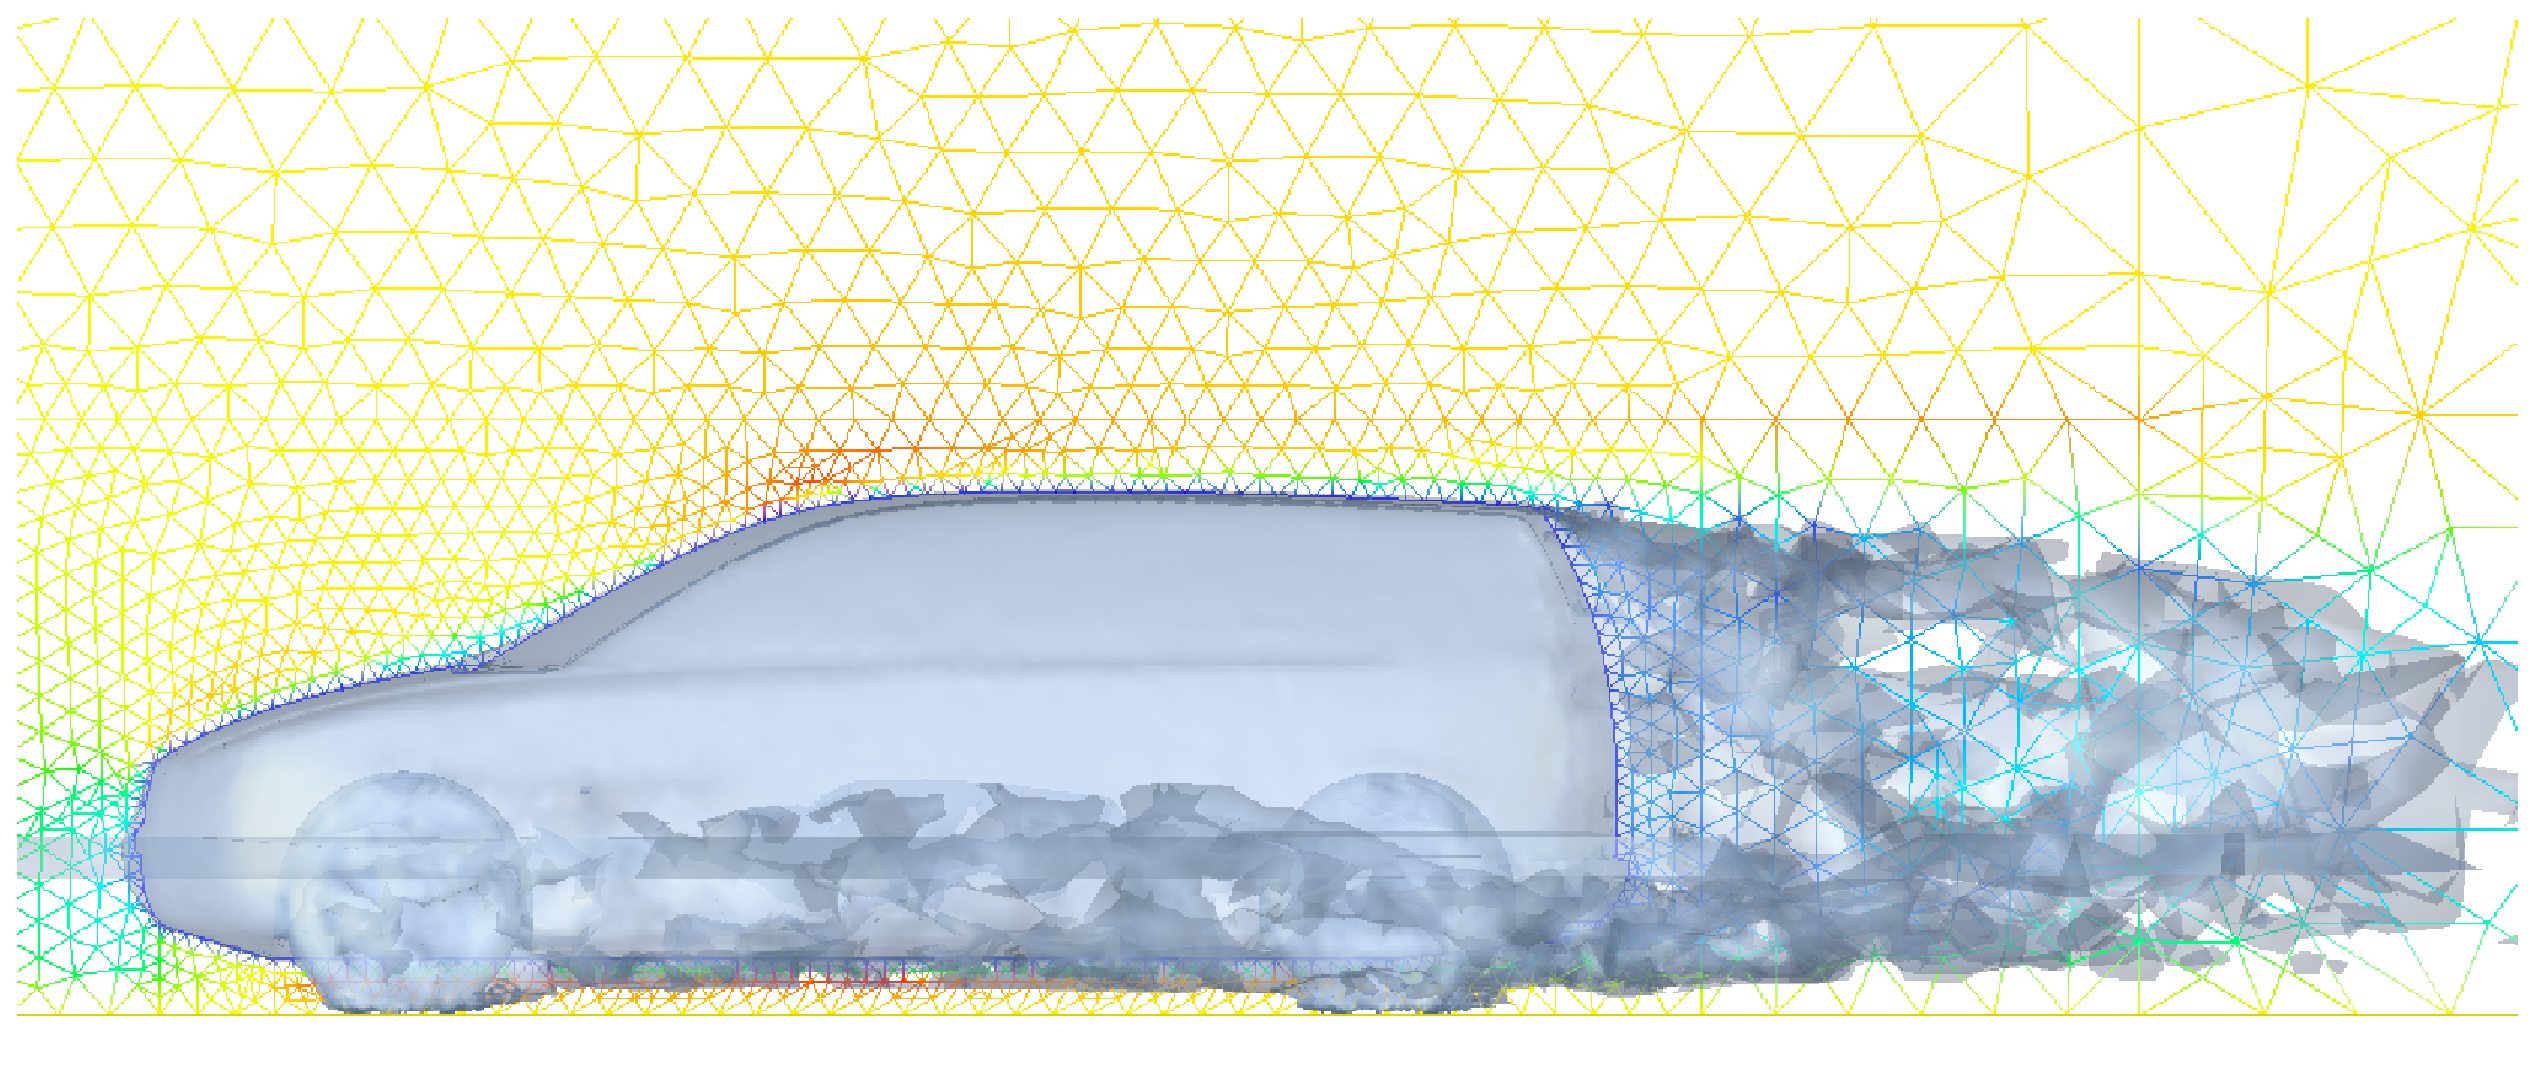
\includegraphics[height=4.5cm]{ambsthermopict/vcc5.eps} 
} 
\caption{Turbulent flow around a car generating drag.}
\label{nse_people} 
\end{figure}
 

An RNS solution 
is a representative of a family of RNS solutions on different
meshes. We are interested in quantitive aspects 
or \emph{outputs} of RNS solutions, which converge under mesh refinement
referred to as \emph{stable outputs}. We will find that
\emph{global mean values} such as \emph{drag} (resistance to
motion)  and \emph{lift}, are stable outputs and thus
are not sensitive to the mesh once sufficiently fine,
while pointwise outputs are unstable. We can thus
view RNS as a new form of (real) continuum model for which solutions
are computable, while the unsolvable Euler equations
represent a formal continuum model without output. It is
the combination of the Euler equations with finite precision
computation which gives valuable output. 


We discover that RNS solutions of the Euler equations  
are \emph{turbulent} and have \emph{shocks} reflecting that
pointwise solutions are lacking.
We find that both turbulence and shocks cause a
transfer of large scale kinetic energy into small scale kinetic
energy in the form of heat, also referred to as 
\emph{turbulent dissipation}, which can be viewed 
as a penalty paid in kinetic energy from pointwise violation 
of conservation of momemtum.  

Note that we do not start from
the \emph{Navier-Stokes equations} already containing viscous
dissipation \emph{by assumption}, which would be analogous to Boltzmann's 
assumption of molecular chaos. Effects of viscous dissipation 
in RNS arise from an \emph{impossibility} in turbulent flow
of achieving a small momentum residual, with the resulting penalty 
acting \emph{like a viscosity}. The viscous dissipation in turbulent RNS 
flow thus can understood as an effect 
of finite precision computation, while the (true) nature of  
physical viscosity has shown to be difficult to unmask.
Without residual stabilization,
computation of RNS solutions show to be impossible 
in the presence of turbulence and shocks. 
With stabilization RNS solutions can be computed and show to accurately
describe thermodynamics including turbulence and shocks.
  



\section{Regularization, Finite Precision and Stability}

RNS solutions can be viewed as pointwise solutions to
regularized perturbed Euler equations with a specific
regularization resulting from least squares residual-based
stabilization directly connecting penalty to violation.


We show that RNS solutions satisfy a 2nd Law, as a consequence
of the 1st Law and stabilization. We can view the 2nd Law to 
express an interplay of \emph{stability} and
\emph{finite precision computation} expressing that unstable processes require
infinite precision for exact execution, and thus cannot be realized,
while stable processes only require finite precision and thus can be realized. 

To smash
a (very expensive very old) Chinese vase into pieces (e.g. by mistake dropping
it on the floor), does not require much of precision, 
while reversing the process and reassembling all the little
pieces would require a very high precision.   

Stability is here related
to the process output. The result of smashing a vase is a smashed vase
and the precise location of the pieces is irrelevant. This allows
quick low precision (brutal) smashing: No matter how you smash, the output is a
smashed vase. On the other hand, the output of the 
reverse restoration process is the original vase, 
and to achieve this result slow high precision (careful) assembly is required. 
So even if in a pointwise sense
both the smashing and the assembly are unstable, the smashing is stable
in the sense that the output of a smashed vase can be quickly be
achieved with low precision. Reversing the smashing in time would 
involve quick high-precision assembly, which cannot be done, and
thus smashing is an irreversible process. This is the essence
of the new 2nd Law in a nutshell illustrating its basic 
ingredients of (output) stability and 
finite precision.

If you do not have an expensive Chinese vase to spare, you can
instead drop a stone to the ground and notice
that it heats up as the (large scale) potential energy of the stone
is converted first to (large scale) kinetic energy as the stone falls
and picks up speed,
and then at impact is converted to (small scale) kinetic energy
perceived as heat, cf. Fig \ref{impact}. 
To get a noticable temperature increase you 
may have to repeatedly drop the stone. In each drop the total
energy is conserved as the large scale potential energy is 
transformed to small scale kinetic energy in the form of heat
energy. Reversal of the process would
involve a stone lifting itself by cooling off, a phenomenon
nobody has ever observed: The reason is that the precision
required to coordinate the small scale heat energy 
into large scale potential energy cannot be attained in a physical
process (while the forward process of dropping the stone does not 
require much of precision).

 
We shall find that turbulent flow has a particular form of
\emph{output stability} with mean-values being stable and
thus computable, while point-values are unstable and thus uncomputable.
This is evidenced in \emph{duality-based posteriori error estimation},
where the stability
of mean-value outputs of shock/turbulent flow results from
\emph{cancellation} in an associated dual problem with 
\emph{highly oscillating coefficients} reflecting the complexity of turbulent 
flow. This fits with the observation that the World 
of thermodynamics is complex and pointwise chaotic, but
because of the complexity, mean-value order can develop from 
pointwise chaos. 

The fact that mean-values are stable and computable 
thus results form the complexity of turbulent flow:

\begin{itemize}
\item  \emph{Complex (turbulent) structures are stable and thus exist}.
\item \emph{Simple (laminar) structures are unstable and thus do not exist.}
\end{itemize} 
This fits with the observation that the existing  world 
of thermodynamics is complex and not simple.


RNS thermodynamics represents a form of deterministic 
chaos, where the mechanism is open to inspection and can be 
used for prediction. Statistical mechanics is based on ad hoc 
assumption not open to inspection, and is difficult to 
use for prediction. 

We shall see that turbulence/shocks appear as a consequence of 
an impossibility to satisfy the Euler equations in a pointwise sense:
This is like a wave building up when approaching a shore
and eventually, when it cannot build up any more, breaks
up into a turbulent cascade in which the large scale kinetic energy
of the coherent wave is transformed into small scale incoherent heat energy,
in an obviously irreversible process. 


The aspect of sharpening or increasing gradients in a wave building
up, which preceeds the resolution 
into a turbulent cascade,  is a fundamental aspect of 
the stability of irreversible processes and closely couples to finite
precision: It is the finite precision which sets a limit
to the sharpening and ultimately forces the process to choose the
only option available in an impossible situation: turbulent dissipation.  



\begin{figure}[bhpt] 
\centerline{ 
\includegraphics[height=8.0cm]{theoryoftimepict/breakingwave2.eps} 
} 
\caption{The irreversible process of a breaking wave illustrates
the 2nd Law.}
\label{breakingwave2} 
\end{figure}
 
 


\section{Finite Precision vs Uncertainty}

The idea that the World performs some form of analog  finite precision 
computation when evolving from one time instant to the next, may seem
new (and repugnant) to physicists.  But this is not necessary, since
the pillars of modern physics, statistical mechanics and quantum mechanics,
both involve \emph{uncertainty} of microscopics, 
which can be viewed as a form of finite precision.    
Thus, both finite precision computation in the form of RNS
and statistical/quantum mechanics involve an 
essential aspect of modern physics of 
\emph{imprecision of microscopics}. An advantage of finite precision
computation is that no data on statistical distributions is required,
only deterministic data.



\section{Internal Energy or Heat Energy}

Heat energy is also referred to as \emph{internal energy}. The
new 2nd Law expresses a transfer of kinetic
energy into internal energy. The irreversibility of this process
means that kinetic energy once converted to ``internal'' energy,
cannot be retrieved and thus is ``lost'': The energy has been
locked in ``internally''. We shall understand below that
this is because small kinetic (internal) energy cannot
be coordinated (because of finite precision) in a reversed process of 
recovering large scale kinetic energy. 
Thus the term ``internal'' seems to capture the physics in a suggestive
metaphor.

We shall see that the new 2nd Law in a way is not new, since it is
so completely basic and results from an energy balance obtained by
the basic operation of multiplication of the momentum equation
by the velocity combined with the finite precision computation
of RNS as a specific form of regularization.  Yet the new 2nd Law is 
non-standard and thus (surprisingly so), in fact in a certain sense is new,
in particular when seen as an interplay of stability and finite precision. 
A basic observation is that generically $D>0$ because of the presence of 
turbulence/shocks in all inviscid flow, except trivial flow
with constant velocity. 

The novelty of the new 2nd Law thus can (and hopefully will) be debated, 
since it is so completely basic, but it is undeniable that it can replace the 
classical 2nd Law without any reference to entropy, 
and is a consequence of the 1st Law and certain finite precision
computation, which appears to 
be genuinely new and open to a simplification of the difficult subject 
of classical thermodynamics.




\section{Maxwell's Demon and Separation}

\emph{Mixing} can be done quickly with low precision (brutally),
while \emph{unmixing/separation} must be done with high precision and 
thus must be slow, if at all feasible.
Compare quickly mixing milk into your coffee with a spoon 
with the impossible reversed process. 
Quick (brutal) mixing is irreversible. But what about slow mixing,
is it also irreversible? Is slow unmixing possible?  

This connects to \emph{Maxwell's Demon} who is supposed to separate/unmix slow
gas molecules from fast ones through a gate allowing only fast molecules 
to pass. Because all fast molecules would have to pass through the gate,
one by one, the separation would have to be slow, since the molecules
would only present themselves by some natural process at the gate
and could not be quickly forced through the gate by the Demon.
Maxwell's Demon could thus be expexted to reverse slow mixing but not
fast mixing.

Now, does Maxwell's Demon exist? Are there processes of slow 
unmixing/separation?
Yes, in Nature there are two basic processes of slow unmixing:
\emph{sedimentation} in geology and \emph{osmosis} in biology,
both contradicting the popular science version of 2nd Law stating that 
``everything has a tendency to disperse'', which we met above.

In sedimentation in the sea, gravitation makes certain particles
fall to the bottom quicker than others, which (very slowly) produces
layers of different material. In osmosis a solvent like water
moves through a semi-permeable membrane from a solute of small
concentration to a solute of higher concentration. Osmosis is the mechanism
through which a tree can suck up water from the ground all the way to
the top of the tree, and thus separate water out of the ground into
the cells. 

Unmixing/separation is a form of \emph{sorting}. We know that 
\emph{digital sorting}
can be made quickly with high precision by computers, but is   
quick analog sorting possible? Yes, a high speed \emph{separator}
can do the job essentially by a process of sedimentation 
driven by strong inertial forces from quick rotation. But biology has
not developed high speed separators, which make many biological processes
irreversible. And a high speed separator does not exactly reverse a process
of mixing.
 
We understand that separation of a substance out of
a mixture with other substances, involves \emph{identification}
and \emph{transport} of the substance. This can be performed quickly 
in digital form, if the process is digitized, but in analog form only slowly,
by processes like sedimentation or osmosis.  

\section{Mixing-Unmixing vs Precision}

We note that a process of mixing
\begin{itemize} 
\item[(m1)] decreases macroscopic difference,
\item[(m2)] increases microscopic difference,
\end{itemize}
while a process of unmixing   
\begin{itemize} 
\item[(u1)] increases macroscopic difference,
\item[(u2)] decreases microscopic difference.
\end{itemize}
We understand that both (m1) and (m2) and also (u1) may be performed with 
low precision, while (u2) requires high precision on microscopic scales
for identification and separation, which in analog form cannot be quick.
Thus quick mixing cannot be reversed. 

\begin{figure}[bhpt] 
\centerline{ 
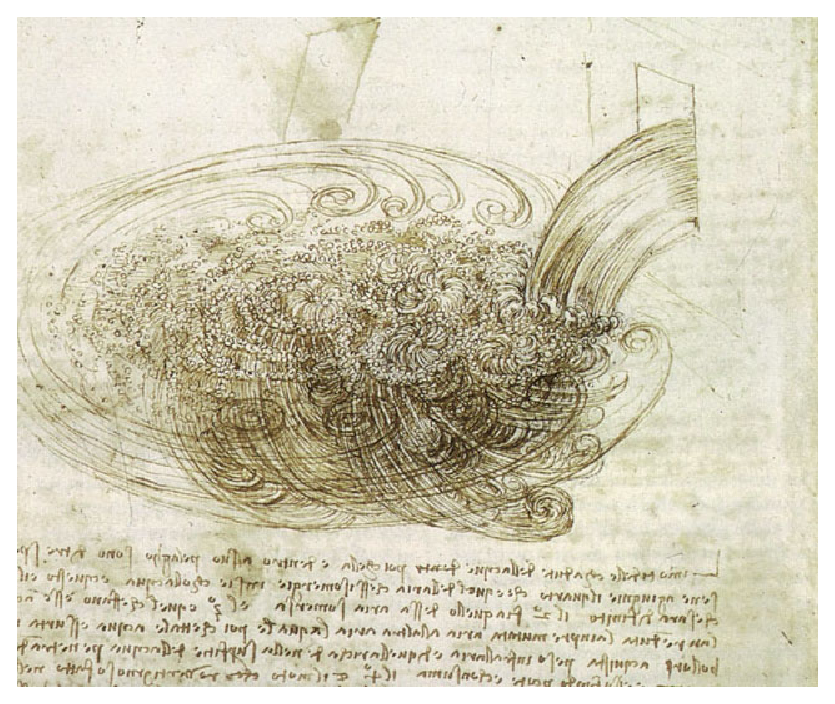
\includegraphics[height=6.0cm]{ambsthermopict/leonardowaterstudy.eps} 
} 
\caption{Emergence of organized structures in turbulent flow
according to Leonardo da Vinci.}
\label{nse_people} 
\end{figure}





   











   








\small
\begin{quote} The second law of thermodynamics is, without a doubt, one of 
the most perfect laws in physics. Any reproducible violation of it, however 
small, would bring the discoverer great riches as well as a trip to Stockholm. 
The world's energy problems would be solved at one stroke. It is not 
possible to find any other law (except, perhaps, for super selection rules 
such as charge conservation) for which a proposed violation would bring more 
skepticism than this one. Not even Maxwell's laws of electricity or 
Newton's law of gravitation are so sacrosanct, for each has measurable 
corrections coming from quantum effects or general relativity. The law 
has caught the attention of poets and philosophers and has been called t
he greatest scientific achievement of the nineteenth century. Engels 
disliked it, for it supported opposition to Dialectical Materialism, 
while Pope Pius XII regarded it as proving the existence of a higher being.
(Bazarov in \emph{Thermodynamics}, 1964)
\end{quote}
\begin{quote}
There is at present in the material world a universal tendency to the 
dissipation of mechanical energy. --- We have the sober scientific 
certainty that 
the heavens and earth shall ``wax old as doth a garment.'' ---
Although mechanical energy is indestructible, there is a universal tendency 
to its dissipation, which produces throughout the system a gradual 
augmentation and diffusion of heat, cessation of motion and exhaustion 
of the potential energy of the material Universe. ---
Any restoration of mechanical energy, without more than an equivalent 
of dissipation, is impossible in inanimate material processes, and is 
probably never effected by means of organized matter, either endowed 
with vegetable life, or subjected to the will of an animated creature.
 --- Nothing can be more fatal to progress than a too confident reliance 
on mathematical symbols; for the student is only too apt to take the 
easier course, and consider the formula not the fact as the physical 
reality. --- I have no satisfaction in formulas unless I feel their 
numerical magnitude.
(Lord Kelvin)
\end{quote}
\normalsize




\fi  % --- end removed block (Classical vs New 2nd Law + RNS as Turbulence Model) ---

\chapter{RNS}
\small

\begin{quote} The 2nd Law cannot be derived from purely mechanical
laws. It carries the stamp of the essentially statistical nature of heat.
(Bergmann \cite{bergmann})
\end{quote}
\begin{quote}
Therefore I feel that the Heisenberg-Bohr (Copenhagen)
statistical interpretation of quantum mechanics is dead. 
(Zeh \cite{zeh})
\end{quote}
\begin{quote}
If a scientist says that something
is possible he is almost certainly right, but if he says that it is
impossible he is probably wrong. (Arthur C. Clarke)
\end{quote}
\normalsize


\section{Introduction}
We refer to \cite{ambsflow} for a detailed presentation of 
RNS for the incompressible Euler equations. The extension 
to the compressible Euler equations has the principal form:
Find $\hat u\in V_h$ such that 
\begin{equation}\label{RNSgen}
((R(\hat u),\hat v))+((hR(\hat u),R'(\hat u,\hat v)))=0\quad \mbox{for }\hat v\in V_h
\end{equation}
where $V_h$ is a space-time finite element space on
a mesh with mesh size $h$, $((\cdot ,\cdot ))$ denotes
space-time $L_2$ scalar products, and $R'(\hat u,\hat v)$ 
is a linearization of the Euler residual $R(\hat u)$ at $\hat u$ 
such that $R'(\hat u,\hat u)=R(\hat u)$, which leads to residual
least squares stabilization 
through the positive penalty term $((hR(\hat u),R(\hat u))$
obtained choosing $\hat v=\hat u$.

In the actual implementation of RNS on cG(1)cG(1)-form stated below,
the stabilisation
has a reduced form involving only some of the terms summing
to the residual. The rationale is that the stabilisation 
has an effect
when the residual is large pointwise, and then stabilising 
one term of the residual suffices. A residual-based 
\emph{shock-capturing} stabilisation with viscosity coefficient
$\sim h^2\vert R(\hat u)\vert$  is also used, which eliminates (small)
oscillations at shocks, but shock-capturing alone is not sufficient.

The 2nd Law satisfied by RNS 
shows that the stabilisation effectively concerns one term
of the momentum equation,
and not the mass and energy equations. The motivation is
that since the momentum equation will not be pointwise (strongly)
small, only weakly small, a stabilisation is required because the 
the balance of kinetic energy results from multiplication 
of the momentum equation by the velocity and this
operation is not stable under weak convergence to zero of the momentum residual.
On the other hand, the mass and energy equations are not similarly
multiplied by density and energy, and thus do not need 
(the same form) of stabilization. 
 

\section{RNS in cG(1)cg(1) Form}



RNS in cG(1)cG(1)-form for the Euler equations (\ref{euler3d1}) 
is a time-stepping method defined by 
find $\hat u =(\rho ,m,e )\in V_h$ such that for all 
$(\bar\rho ,\bar u,\bar e )\in W_h$
\begin{equation}\label{RNS}
\begin{split}
((R_\rho (\hat u),\bar\rho ))+((\delta u\cdot\nabla\rho , 
u\cdot\nabla\bar\rho ))&=0,\\
((R_m(\hat u),\bar u))+
((\delta \rho u\cdot\nabla u, u\cdot\nabla\bar u))&=0,\\
((R_e (\hat u),\bar e ))+
((\delta u\cdot\nabla e ,u\cdot\nabla\bar e ))&=
((d_h,\bar e)),
\end{split}
\end{equation}
where
\begin{equation}\label{dh}
d_h=\sum_{i=1}^3\delta \rho(u\cdot\nabla u_i)^2,
\end{equation}
and $V_h$ is a trial space of continuous piecewise linear 
functions on a space-time mesh of size $h$ satisfying the initial
condition $\hat u(0)=\hat u^0$ with $u\in V_h$ defined by
nodal interpolation of $\frac{m}{\rho}$, and $W_h$ 
is a corresponding test space of function which are
continuous piecewise linear in space and piecewise constant in time,
all functions satisfying the boundary condition $u\cdot n=0$ at the 
nodes on $\Gamma$. The space-time mesh is organised 
into space-time slabs between discrete time levels, and  
the velocity in the stabilisation terms is averaged over each time step.
Further, $((\cdot ,\cdot ))$  denotes relevant  
$L_2(Q)$ scalar products. Finally, the least squares
stabilisation weight 
$\delta=\frac{ch}{\vert u\vert}$ with $c\approx 0.5$,
and \emph{shock-capturing viscosity}
with viscosity coffecient 
$\nu_i\sim h^2\vert R_i(\hat u)\vert^2$, $i=\rho ,m,e,$ is also added
to each equation separately, which eliminates 
the small oscillations occuring at shocks with only
least squares stabilisation. For small densities (almost vacuum), the
velocity is computed by $u=\frac{m}{\rho +\epsilon}$ with
$\epsilon >0$ suitably small.
 
RNS (\ref{RNS}) combines a weak satisfaction of the Euler equations
with in particular a weighted least squares control of (a part of) the 
momentum residual $R_m(\hat u)$ and
represents a midway between the Scylla of weak solution and
Carybdis of least squares strong solution. 

Including all terms of the residual in the stabilisation as indicated in (\ref{RNSgen}) improves consistency and 
thus may improve accuracy. Because test functions are piecewise constant in time the time derivative term
will be missing in the residual stabilisation, however without much degrading accuracy in the presence of turbulence and shocks.

The form of the
stabilisation terms in the density and energy equations
secures exact global conservation since
the stabilisation terms vanish with $\bar\rho =\bar e \equiv 1$.
Notice that choosing $\bar\rho =\rho$ (mean-value
over time step) gives a bound on 
$\int_Q\delta (u\cdot\nabla\rho )^2dxdt$ in terms of 
$\int_Q\rho^2\nabla\cdot udxdt$, with a similar
control of $e$.

Notice that RNS as expressed in (\ref{RNS}) has a remarkable simplicity,
as compared to finite difference methods based on diagonalization
of the full system together with
Riemann solvers, and also compared to stabilized finite element methods
using diagonalization of the full linearized operator. In (\ref{RNS})
each scalar convection equation is stabilized separately 
without diagonalization. In particular, the net numerical 
dissipation $d_h$ has a contribution from each
separate momentum/velocity component, but there is no net
numerical dissipation in mass and internal energy.

\section{The 2nd Law for RNS}

Choosing $\bar u$ in the momentum equation as
the time average of $u$ over the time step, and subtracting
the mass equation with $\bar\rho =I_h(\frac{\vert u\vert^2}{2})$, where
$I_h(\frac{\vert u\vert^2}{2})$ is a nodal interpolant
of $\frac{\vert u\vert^2}{2}$, we obtain 
\begin{equation}\label{2ndlawRNSK}
\dot K = W-D_h,
\end{equation}
where 
\begin{equation}
D_h=\int_Qd_h\, dxdt,
\end{equation}
modulo the additive term
\[
I=\vert ((R_\rho ,\frac{\vert u\vert^2}{2}-I_h(\frac{\vert u\vert^2}{2})))\vert
\]
which  by super-approximation as in \cite{ambsflow}
can be estimated as follows, 
\[
I\le C\Vert h^2 R_\rho (\hat u)\vert\nabla u\vert^2\Vert_0,
\]
where $\Vert\cdot\Vert_0$ is the $L_2(Q)$-norm and $C\sim 1$ 
is an interpolation constant.
Assuming $\vert R_\rho (\hat u)\vert\sim h^{-1/2}$ and  
$\vert\nabla u\vert\sim h^{-1/2}$,
we obtain $I\sim \sqrt{h}$, indicating that
$I$ is a small perturbation, which in computation can be
checked a posteriori. Finally choosing in the equation for 
internal energy $\bar e=1$, we obtain 
\[
\dot E=-W+D_h,
\]
and we thus obtain the following 2nd Law for RNS 
(modulo a $\sqrt{h}$ correction)
\begin{equation}\label{2ndlawRNS}
\dot K = W-D_h,\quad\dot E=-W+D_h.
\end{equation}
For solutions with turbulence/shocks, $D_h>>0$ expressing a substantial 
irreversible transfer of kinetic energy into heat energy, 
just as above for regularized
solutions. We note that in RNS only the momentum equation is
subject to viscous regularization, since $D_h$ expresses a 
penalty on the term $u\cdot\nabla u_i$ appearing in the momentum residual.
A turbulent solution is identified by $D_h\sim 1$ under mesh refinement.  

\section{The Stabilization in RNS}

%The precise form of RNS used in the computations,
%is a stabilized form of cG(1) with continuous piecewise
%linear trial functions in space-time and test functions which
%are piecewise linear in space and piecewise constant in time.
We have seen that the stabilization in RNS is expressed 
by the dissipative term $D_h\sim 1$ 
which can be viewed as a weighted least squares control
of the term $\rho u\cdot\nabla u_i$ in the momentum residual.
The rationale is that least squares control of a  
part of a residual which is large, effectively may 
give control of the entire residual, and thus RNS 
gives a least squares control of the 
momentum residual. But the RNS stabilization does not correspond
to an ad hoc viscosity, as in classical regularization, but to
a form of penalty arising because Euler residuals 
of turbulent/shock solutions \emph{cannot} be pointwise small. 

In particular
the dissipative mechanism of RNS does not correspond to a
shear viscosity acting in all directions, 
as in standard ad hoc regularization, but rather to a form of 
bulk viscosity in the form of \emph{streamline diffusion}
preventing fluid particles from colliding while allowing strong shear,
%RNS also contains residual dependent 
%\emph{shock-capturing viscosity}, of minor importance in the present
%context, see \cite{ambsthermo}.
connecting to the \emph{streamline diffusion method}  
presented in \cite{cde}.      









\chapter{Output Wellposedness by Duality}

\small
\begin{quote} In love all the contradiction of existence merge themselves 
and are lost. Only in love are unity and duality not at variance. 
Love must be one and two at the same time. Only love is motion and rest 
in one. (Rabindranath Tagore, Literature Nobel Prize 1913)
\end{quote}

\begin{quote}
Those who have talked of ``chance'' are the
inheritors of antique superstition and ignorance...whose minds have never
been illuminated by a ray of scientific thought. (T. H. Huxley)
\end{quote}
%\begin{quote} Emergence means complex organizational structure growing out
%of simple rules. Emergence means stable inevitability in the way certain
%things are. Emergence means unpredictability, in the sense of small events
%causing great and qualitative changes in larger ones. Emergence means the
%fundamental impossibility of control. 
%(Robert Laughlin in A Different Universe,
%2005)
%\end{quote}
\normalsize


\section{A Posteriori Error Estimation} 

Consider a mean-value output $M(\hat u)$ in the form of a space-time integral
\begin{equation}
M(\hat u)=((\hat u,\hat\psi ))
\end{equation}
defined by a smooth (positive) weight function $\hat\psi$ with 
$\Vert\psi\Vert_0=1$, where as above $\Vert\cdot\Vert_0$ is the $L_2(Q)$-norm.
Let $\hat u$ and $\hat w$ be 
two RNS solutions on two meshes with joint maximal meshsize $h$.
By the mean-value theorem their residual difference can be expressed
as
\[
R(\hat u)-R(\hat w)=R'(\hat u,\hat w)\cdot (\hat u-\hat w),
\]
where $R'(\hat u,\hat w)$ is a linearization of $R(\cdot )$. Letting  
$\hat\varphi$ be the solution of the dual linearized equation
\begin{equation}\label{dual}
R'^\top\hat \varphi =\hat\psi,
\end{equation}
where $\top$ denotes transpose, 
we obtain the following basic \emph{output error representation}:
\begin{equation}\label{errorrepr}
M(\hat u)-M(\hat w)=((\hat u-\hat w,R'^\top\hat\varphi ))=((R(\hat u)-R(\hat w),\hat\varphi )).
\end{equation}
We can thus estimate the output error in terms of the residuals as
follows: 
\begin{equation}\label{apost1}
\vert M(\hat u)- M(\hat w\vert\le S
(\Vert R(\hat u)\Vert_{-1}+(\Vert R(\hat w)\Vert_{-1})
\end{equation}
or alteratively, using also \emph{Galerkin orthogonality} as in \cite{ambsflow} 
\begin{equation}\label{apost0}
\vert M(\hat u)- M(\hat w\vert\le S
%(\Vert R(\hat u)\Vert_{-1}+(\Vert R(\hat w)\Vert_{-1})
(\Vert h R(\hat u)\Vert_{0}+(\Vert h R(\hat w)\Vert_{0}) ,
\end{equation}
where
\begin{equation}\label{Suw}
S=S(\hat u,\hat w)=\Vert\hat\varphi\Vert_1
\end{equation}
with $\Vert\cdot\Vert_1$ the $H^1(Q)$-norm.

For a given output $M(\hat u)$, we choose an error tolerance 
$TOL$ and define a RNS-solution $\hat u$ to be \emph{wellposed}
up to the tolerance $TOL$, if  
\begin{equation}\label{tol1}
S\Vert h R(\hat u)\Vert_{0}\le TOL/2 ,
\end{equation}
where $S=S(\hat u,\hat u)$. Given two wellposed RNS solutions $\hat u$ and
$\hat w$, we may expect
\begin{equation}\label{tol2}
\vert M(\hat u)- M(\hat w\vert\le TOL ,
\end{equation}
up to a variation of the corresponding stability factors, which
can be computed a posteriori. A solution which is not wellposed
with respect to some tolerance of interest, is said to be \emph{illposed}.
 



Turbulence is characterized  by 
\begin{equation}\label{Dh1}
D_h\sim\Vert\sqrt{h} R(\hat u)\Vert_{0}\sim 1
\end{equation}
under mesh refinement. We may thus expect an output $M(\hat u)$ 
to be \emph{wellposed} up to the tolerance $TOL$ if 
\begin{equation}\label{Su}
S(\hat u,\hat u)\lesssim\frac{TOL}{2\sqrt{h}}.
\end{equation} 
A wellposed output can be uniquely computed up to a tolerance 
$TOL$ of interest,
but an illposed cannot.

Computational results, some of which
is presented below and more on the book web page
\cite{bodysoulmath}, show that indeed 
$\Vert hR(\hat u)\Vert_0\sim \sqrt{h}$ conformiing (\ref{Dh1}),
and that the corresponding stability factors $S(\hat u,\hat u)$
for global mean-values such as drag, lift and total turbulent 
dissipation, can satisfy (\ref{Su}) for toleralnces $TOL$
of interest. In short, global mean-value outputs
can be wellposed, and thus represent stable computable 
emergent aspects of turbulent flow.



\chapter{Linearized Equations and Acoustics}

\small
%\begin{quote}
%It doubtless seems highly paradoxical to assert that Time is unreal, and 
%that all statements which involve its reality are erroneous. Such an 
%assertion involves a far greater departure from the natural position of 
%mankind than is involved in the assertion of the unreality of Space or of 
%the unreality of Matter. So decisive a breach with that natural position 
%is not to be lightly accepted. And yet in all ages the belief in the 
%unreality of time has proved singularly attractive. 
%(John Ellis McTaggart, The Unreality of Time,
%Quarterly Review of Psychology and Philosophy 17 (1908), 456-473.)
%\end{quote}
\begin{quote}
De Broglie, the creator of wave mechanics, accepted
the results of quantum mechanics just as Schr\"odinger did, but not
the statistical interpretation. (Born in the Born-Einstein Letters)
\end{quote}
\normalsize

\section{Linearization}
Consider a solution $\hat u=(\rho ,m,e)$ of the 
Euler equations:
\begin{equation}\label{euler10}
\begin{array}{rcl}
\dot \rho +\nabla\cdot (\rho u) =\dot \rho +\nabla\cdot m &=&  0 \quad \mbox{in } Q, \\
\dot m+\nabla\cdot (mu) + \gamma\nabla e&=&  f \quad \mbox{in } Q, \\
\dot e +\nabla\cdot (eu)+\gamma  e\nabla\cdot u &=& g  \quad \mbox{in } Q,\\ 
u\cdot n&=&0\quad \mbox{on } \Gamma\times I\\
\hat u(\cdot ,0)&=&\hat u^0\quad \mbox{in } \Omega , 
\end{array} 
\end{equation}
where $u=\frac{m}{\rho}$.
The corresponding \emph{linearized Euler equations}, linearized at $\hat u$,
take the following form in
$\underline{\hat u} =(\underline{\rho},\underline{m},\underline{e})$
representing a perturbation of $\hat u$ with corresponding 
perturbation of data, with $\underline{u}$ defined
by $\underline{m}=\underline{\rho}u+\rho\underline{u}$:
\begin{equation}\label{lineuler1}
\begin{array}{rcl}
\underline{\dot\rho} 
+\nabla\cdot (\underline{\rho}u)+\nabla\cdot (\rho\underline{u})=\underline{\dot\rho} +\nabla\cdot\underline{m}
%\nabla\cdot (\rho\underline{u})
%-\nabla\cdot (m\frac{m}{\rho^2})--\nabla\cdot (e\frac{m}{\rho^2}) 
&=& 0\quad \mbox{in } Q, \\
\underline{\dot m} +\nabla\cdot (\underline{m}u)+
\nabla\cdot (m\underline{u})
+ \gamma\nabla\underline{e}&=&  \underline{f} \quad \mbox{in } Q, \\
\underline{\dot e} +\nabla\cdot (\underline{e} u )
+\nabla\cdot (e\underline{u})+\gamma\underline{e}\nabla\cdot u
+\gamma e\nabla\cdot\underline{u} &=& \underline{g}  \quad \mbox{in } Q,\\ 
\underline{u}\cdot n&=&0\quad \mbox{on } \Gamma\times I,\\
\underline{\hat u}(\cdot ,0)&=&\underline{\hat u}^0\quad \mbox{in } \Omega , 
\end{array} 
\end{equation}
or alternatively with $Dw=\dot w+u\cdot\nabla w$ the $u$-convective
derivative:
\begin{equation}\label{lineuler2}
\begin{array}{rcl}
D\underline{\rho} +\underline{\rho}\nabla\cdot u 
+\nabla\cdot (\rho\underline{u})&=&  0 \quad \mbox{in } Q, \\
D\underline{m} + \underline{m}\nabla\cdot u +
\nabla\cdot (m\underline{u})
+ \gamma\nabla\underline{e}&=&  \underline{f} \quad \mbox{in } Q, \\
D\underline{e} 
+\underline{u}\cdot\nabla e+(\gamma +1)\underline{e}\nabla\cdot u
+(\gamma +1) e\nabla\cdot\underline{u} &=& \underline{g}  \quad \mbox{in } Q,\\ 
\underline{u}\cdot n&=&0\quad \mbox{on } \Gamma\times I\\
\underline{\hat u}(\cdot ,0)&=&\underline{\hat u}^0\quad \mbox{in } \Omega .
\end{array} 
\end{equation}
This is a linear convection-reaction system with coefficients 
depending on the base flow $\hat u$ and the stability properties of 
this system govern the perturbation growth.


\section{Wave Equation}
Let $\hat u$ be a constant ground state
with velocity $u=0$ and temperature $\tau =1$. If  
$\tau$ is not subject to perturbation, so that $\underline{e} =
\underline{\rho}$, then (\ref{lineuler1}) reduces
to (leaving out initial and boundary conditions):
\begin{equation}\label{wave1}
\begin{array}{rcl}
\underline{\dot\rho} +\nabla\cdot\underline{m}
%\nabla\cdot (\rho\underline{u})
%-\nabla\cdot (m\frac{m}{\rho^2})--\nabla\cdot (e\frac{m}{\rho^2}) 
&=& 0\quad \mbox{in } Q, \\
\underline{\dot m}
+ \gamma\nabla\underline{\rho}&=&  \underline{f} \quad \mbox{in } Q, \\
%\underline{\dot e} +\nabla\cdot (\underline{e} u )
%+\nabla\cdot (e\underline{u})+\gamma\underline{e}\nabla\cdot u
%+\gamma e\nabla\cdot\underline{u} &=& \underline{g}  \quad \mbox{in } Q,\\ 
%\underline{u}\cdot n&=&0\quad \mbox{on } \Gamma\times I,\\
%\underline{\hat u}(\cdot ,0)&=&\underline{\hat u}^0\quad \mbox{in } \Omega , 
\end{array} 
\end{equation}
which leads to the \emph{wave equation} for the density perturbation, assuming 
$\nabla\cdot\underline{f}=0$:
\begin{equation}\label{wave2}
\underline{\ddot\rho}-\gamma\Delta\underline{\rho}=0 \quad \mbox{in } Q.
\end{equation}
Small density-pressure variations at constant
temperature around a constant ground state thus
obeys the linear wave equation with wave speed $c=\sqrt{\gamma}$.

Allowing a non-zero velocity of the ground state,
but still constant unit temperaure, the linearized 
equations reduce to (assuming $\underline{e}=0$):
\begin{equation}\label{wave1}
\begin{array}{rcl}
\underline{\dot\rho} +\nabla\cdot\underline{m}
%\nabla\cdot (\rho\underline{u})
%-\nabla\cdot (m\frac{m}{\rho^2})--\nabla\cdot (e\frac{m}{\rho^2}) 
&=& 0\quad \mbox{in } Q, \\
\underline{\dot m}+2\nabla\cdot (\underline{m}u)-
\nabla\cdot (\underline{\rho}uu)
+ \gamma\nabla\underline{\rho}&=&  \underline{f} \quad \mbox{in } Q, \\
%\underline{\dot e} +\nabla\cdot (\underline{e} u )
%+\nabla\cdot (e\underline{u})+\gamma\underline{e}\nabla\cdot u
%+\gamma e\nabla\cdot\underline{u} &=& \underline{g}  \quad \mbox{in } Q,\\ 
%\underline{u}\cdot n&=&0\quad \mbox{on } \Gamma\times I,\\
%\underline{\hat u}(\cdot ,0)&=&\underline{\hat u}^0\quad \mbox{in } \Omega , 
\end{array} 
\end{equation}
which is a generalized wave equation with contributions from 
convection with velocity $u$.


\section{Acoustics}

\emph{Acoustics} concerns propagation of
(usually small) density-pressure variations in a fluid.
Acoustics simulation can be based on (i) directly solving the 
Euler equations for the 
full state (ground state plus perturbation), or (ii) solving
the Euler equations for the ground state followed by  
solution of the linearized Euler equations for the perturbation with the
ground state given. We just saw that the simplest model
for acoustics is the wave equation (\ref{wave2}) as a basic case of (b). 
In general, (ii) may be expected to give higher accuracy at the expense
of solving both the Euler and linearized Euler equations.

The wave equation can be used for progagation of sound waves in
in a fluid at rest, but for the generation of sound in e.g.
human speech or musical instruments, fluid-structure 
interaction is used, which requires the Euler equations for the
(usually turbulent) flow and an elasticity model for the
structure (e.g, vocal chords).  




\section{Linearized Stability}
The nature of the linearized system (\ref{lineuler1}) depends
on the ground state and ranges from its simplest incarnation
in the form of the wave equation (\ref{wave2})
for a constant ground state, to a highly complex problem for 
a turbulent ground state. Below we analyze the linearized 
problem for a shocks and rarefaction waves in a model case,
and in \cite{ambsflow} we discuss the case of turbulent incompressible
flow. For now, we only observe that the equation for $\underline{\rho}$  
contains the term $\underline{\rho}\nabla\cdot u$, and the same for $\underline{m}$ and $\underline{e}$,
which indicates exponential perturbation growth
along particle paths under compression with $\nabla\cdot u <0$,
which occurs when a compression shock is forming.


  
\chapter{Dual Linearized Problem}


\small

\begin{quote}
Those who do not understand the nature of sin and virtue are attached 
to duality; they wander around deluded. (Sri Guru Granth Sahib)
\end{quote}
\normalsize



Formally multiplying the linearized equation (\ref{lineuler1})
by the dual variable $\hat\varphi =(\rho_d,\varphi ,e_d)$
and integrating by parts and varying $\underline{\hat u}$, we
obtain the following dual problem
\begin{equation}\label{dualeuler}
\begin{array}{rcl}
-\dot \rho_d+\sum_{j}(u\cdot\nabla\varphi_{j})\,u_j+\frac{e}{\rho}u\cdot\nabla e_d+\frac{\gamma}{\rho}u\cdot\nabla (ee_d)
&=&  \psi_\rho , \\
-\dot\varphi - u\cdot\nabla\varphi -\sum_iu_i\nabla\varphi_{i}-\nabla\rho_d 
-\frac{e}{\rho}\nabla e_d-\frac{\gamma}{\rho}\nabla (e e_d)&=&  \psi , \\
-\dot e_d -u\cdot\nabla e_d+\gamma\nabla\cdot ue_d-
\gamma\nabla\cdot\varphi &=& \psi_e ,\\ 
%\varphi\cdot n&=&0\quad \mbox{on } \Gamma\times I\\
\end{array} 
\end{equation}
where the data $\hat\psi =(\psi_\rho ,\psi ,\psi_e)$ defines the output.
We check by writing the Euler equations alternatively
in the variables $\hat u=(\rho ,u,e)$:
\begin{equation}\label{euler10uve}
\begin{array}{rcl}
\dot \rho +\nabla\cdot (\rho u )&=&  0, \\
\dot \rho u+\rho\dot u +\nabla\cdot (\rho uu) + \gamma\nabla e&=&  f, \\
\dot e +\nabla\cdot (eu)+\gamma  e\nabla\cdot u &=& g,\\ 
%u\cdot n&=&0\quad \mbox{on } \Gamma\times I\\
%\hat u(\cdot ,0)&=&\hat u^0\quad \mbox{in } \Omega , 
\end{array} 
\end{equation}
with corresponding dual linearized problem 
in $\hat\varphi =(\rho_d, \varphi ,e_d)$:
\[
\begin{array}{rcl}
-\dot \rho_d-u\cdot\nabla\rho_d -u\cdot\dot\varphi -\sum_iu_iu\cdot\nabla\varphi_i 
&=&  \psi_\rho , \\
-\rho\dot\varphi-\rho u\cdot\nabla\varphi -\rho\nabla\rho_d 
-e\nabla e_d-\gamma\nabla (e e_d)-\rho\sum_iu_i\nabla\varphi_{i}&=&  \psi , \\
-\dot e_d -u\cdot\nabla e_d+\gamma\nabla\cdot ue_d-
\gamma\nabla\cdot\varphi &=& \psi_e ,\\ 
%\varphi\cdot n&=&0\quad \mbox{on } \Gamma\times I\\
%\hat\varphi (\cdot ,0)&=&0\quad \mbox{in } \Omega , 
\end{array} 
\]
which by eliminating $\dot\varphi$ from the first equation using
the second gives
\[
\begin{array}{rcl}
-\dot \rho_d+\sum_{j}(u\cdot\nabla\varphi_{j})\,u_j+\frac{e}{\rho}u\cdot\nabla e_d+\frac{\gamma}{\rho}u\cdot\nabla (ee_d)
&=&  \psi_\rho , \\
-\dot\varphi - u\cdot\nabla\varphi -\sum_iu_i\nabla\varphi_{i}-\nabla\rho_d 
-\frac{e}{\rho}\nabla e_d-\frac{\gamma}{\rho}\nabla (e e_d)&=&  \psi , \\
-\dot e_d -u\cdot\nabla e_d+\gamma\nabla\cdot ue_d-
\gamma\nabla\cdot\varphi &=& \psi_e ,\\ 
%\varphi\cdot n&=&0\quad \mbox{on } \Gamma\times I\\
\end{array} 
\]
which is the same as (\ref{dualeuler}) with a properly modified right
hand side: the elimination divides the second equation by $\rho$
(so that $\psi\to\psi/\rho$), and substituting $\dot\varphi$ into the
first equation absorbs the data contribution
$\psi_\rho\to\psi_\rho-\frac{1}{\rho}u\cdot\psi$, while the three
quadratic terms in $u$ combine to the single term
$\sum_j(u\cdot\nabla\varphi_j)\,u_j$.

The dual problem (\ref{dualeuler}) is solved backward in time on $[0,T]$
with e.g. $\hat\varphi (\cdot ,T)=0$, for simplicity with stabilization 
by artificial diffusion of size $h$ in each equation instead
of least squares stabilization. The crucial stability factor
is defined by $S=\Vert\varphi\Vert_{H^1(Q)}/\Vert\psi\Vert_{L_2(Q)}$,
which bounds the error in the output $(\hat u,\psi )_Q$ by 
$S\Vert hR(\hat u)\Vert_{L_2(Q)}$.
 



   


\iffalse  % --- removed in shortened layout: redundant with main RNS chapter ---
\chapter{RNS as a Model of Physics}

\small
\begin{quote}
Die Welt ist alles, was der Fall ist. (Wittgenstein)
\end{quote}
\normalsize
   

\section{A Dissipative Mechanism}

We propose to view RNS as a real model of thermodynamics with output, 
as compared to the Euler equations, which represent a formal model 
without output. 
We have seen that the least squares stabilization introduces
a specific form of viscosity and that an RNS solution 
$\hat u$ has Euler momentum residual $R_m(\hat u)$ typically satisfying
\begin{equation}
\Vert R_m(\hat u)\Vert_{-1}\sim \sqrt{h},\quad \Vert R_m(\hat u)\Vert_0\sim \frac{1}{\sqrt{h}}.
\end{equation}
Roughly speaking this means that local mean-values 
of the Euler momentum residual $R_m(\hat u)$ are small, 
and that point-values not too large. Momentum balance is thus
(heavily) violated locally and then penalized by a viscous dissipative 
mechanism consuming kinetic energy, while momentum balance is satisfied 
in a local mean value
sense. Turbulence creates violent kinetics violating momentum
balance locally, and is countered by a dissipative mechanism on kinetic
energy curbing the violation. RNS flow thus
is out of momentum balance in a pointwise sense but in 
balance in a  mean-value sense. It is thus possible to interprete
RNS in physical terms as a dissipative mechanism 
compensating local imbalance of momentum.   


The reason RNS cannot satisfy pointwise momentum balance is that
the Euler equations lack pointwise solutions. 
Facing the impossibility
of pointwise solution, RNS reacts by producing an approximate
solution in which some of the kinetic energy by turbulent/shock dissipation.
The total dissipation shows to be a stable output under vanishing mesh size
and occurs mainly on the finest scale of the mesh. The turbulent/shock
dissipation thus is ``smart'' and does not act on coarser scales. 

The key here is to realize that
the dissipative stabilization is (i) necessary, (ii) substantial, 
(iii) irreversible, (iii) not
a numerical artifact which can be diminished by increasing
the precision. The key new fact behind (i)-(iv) is the 
non-existence of pointwise solutions to the Euler equations.
Note that (iii) reflects the well-known difficulty of getting
a refund of a fine which has been paid. 


\section{From Exact to Computational Solutions}

The nonexistence of (stable) pointwise solutions to the
Euler equations upsets classical mathematics: With nonexistent
exact solutions, the attention has to move to existing approximate 
solutions, and thus the computational aspect takes 
the lead before analytical mathematics. This suggests 
an entire shift of paradigm, which we can now
only vaguely imagine. 
 

The non-existence of pointwise solutions to the Euler equations, 
which may be viewed as a failure of mathematics, in fact may be turned around
into an advantage from a computational point of view: If there were an exact
solution, one could always ask for more precision 
in computing this solution requiring finer resolution and higher 
computational cost, but if there is no exact solution, 
then we could be relieved from this demand beyond a certain point. 
A key feature in this situation is that the absolute size of the 
fine scales no longer are important, and this could save computational work.
In turbulence this means that mean value outputs may be computed 
on meshes which do not resolve the turbulent vortices to their actual
physical scale.

In order for a Hamiltonian system to develop turbulence, it has
to be rich enough in degrees of freedom. In particular, the incompressible
or compressible Euler equations in less than three 
space dimensions are not rich 
enough, even if the mesh is very fine. On the other hand,
turbulence invariably develops in three dimensions once the mesh is
fine enough. 
%Likewise, a particle system must be free to evolve in (at least)
%three space dimensions and the number of particles will have to be large
%enough. 
Our experience with turbulent solutions of the incompresible
Navier-Stokes equations indicates that a mesh with 100.000 mesh points
in space may suffice in simple geometries, while in more complex geometries 
millions, but not billions, of mesh points may be needed.







 
\section{Imperfect Nature and Mathematics?}

How shall be interprete that the Euler equations do not have 
pointwise solutions? Does this express an imperfection of 
both mathematics and physics? 
We can make a parallel with the squareroot of two $\sqrt{2}$, which is
the length of the diagonal in a square with side length 1.
We know that the Pythagoreans discovered that $\sqrt{2}$ is not a rational
number. This knowledge had to be kept secret, since it indicated
an imperfection in the creation by God formed as relations
between natural numbers according the basic belief of the Pythagoreans. 
Eventually this unsolvable conflict ruined their philosophical school
and gave room for the Euclidean school based on geometry instead of
natural numbers. Civilization did not recover until Descartes
resurrected numbers and gave geometry an algebraic form, which 
opened for Calculus and the scientific revolution.

But how is the Pythagorean paradox of non-existence of $\sqrt{2}$ 
as a rational number handled today? Well, we know that the 
accepted mathematical solution since Cantor and Dedekind is to extend
the rational numbers to the real numbers, some of which like
$\sqrt{2}$ are called irrational, and which can only be described
approximately using rational numbers. We may say that this solution
in fact is a kind of non-solution, since it acknowledges the fact that
the equation $x^2=2$ cannot be solved exacly using rational numbers,
and since the existence of irrational numbers
(as infinite decimal expansions or Cauchy sequences of rational numbers)
has a different nature than the existence of natural numbers or rational
numbers. The non-existence is thus handled by expanding the solution concept
until existence can be assured.

We handle the non-existence of pointwise solutions to the Euler equations 
similarly, that is,
by extending the solution concept to approximate solution
in a weak sense combined with some control of pointwise residuals.
Doing so we necessarily introduce a dissipation causing irreversibility.
In this case, the non-existence of solutions thus has a cost:  
irreversibility. In the perfect World, pointwise solutions would exist,
but this World cannot be constructed neither mathematically nor physically,
and in a constructible World necessarily there will exist irreversible
phenomena as a consequence of the non-existence of pointwise solutions.
The non-existence of pointwise solution reflects the development of
complex solutions with small scales, and thus the non-existence also
relects a complexity of the constructible World. The perfect World
would lack this complexity, so in addition to being non-existent 
it would also probably be pretty non-interesting.  The World we live in thus 
does not seem to be perfect, but it surely is complex and interesting.

An imperfect World of mathematics and physics, where
equations cannot be solved exactly or laws of physics cannot be exactly 
satisfied, is unthinkable to the classical mathematician and 
physicist, but nevertheless seems ``to be the case'' in Wittengenstein's
words. The perfect World ``is not the case'' and thus 
can be only marginal of interest.

The contradiction of a non-existing perfect World, and an existing
imperfect World, has been met by statistical mechanics and quantum mechanics
based on microscopical games of Roulette. We propose to resolve
the contradiction instead by finite precision computation, because
it is simpler and more useful.

\section{Idealism and Materialism}
From philosophical point of view, we may say that the traditional 
paradigm of both mathematics
and physics is Platonistic in the sense that it assumes the existence of an Ideal
World, where 
equations/laws are satisfied exactly. We may say that this is an Ideal World of
infinities 
because exact satisfaction of e.g. the equation $x^2=2$ requires infinitely many
decimals.
This is the mathematical Ideal World of Cantor, which represents a formalist/logicist
school. In strong opposition to this school of infinities, is Brouwer's constructivist
school,
which only deals with mathematicial objects that can be constructed or
computed in a finite number
of steps. In the constructivists Constructible World, the set of natural numbers
does not exist
as a completed mathematical object as in Cantors Ideal World, but only as a
never-ending 
project where always a next natural number can be constructed if needed, which
follows the
suggestions of e.g. Aristotle and Gauss. The Constructible World is finitary and thus
inherently computational, while Cantors Ideal World is non-finitary and
non-computational. 
%We give our vote to the Constructible World, 
%which today can be explored using the
%computer, which is the leading theme of the Body$\&$Soul project.

\begin{figure}[bhpt] 
\centerline{ 
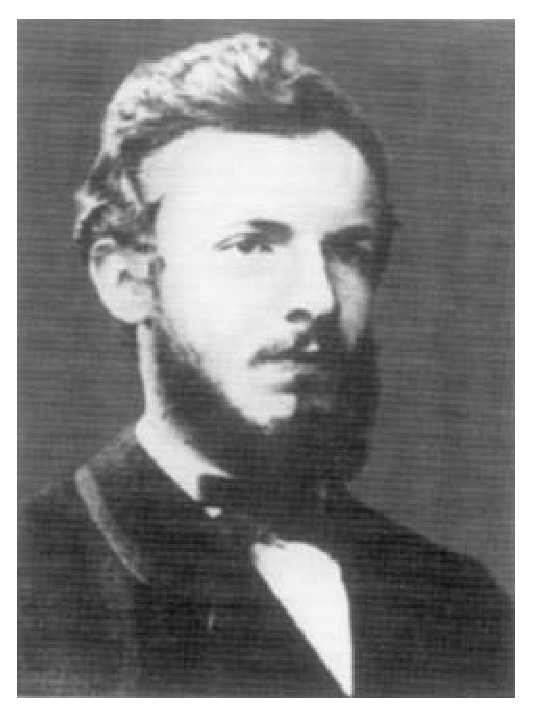
\includegraphics[height=6.0cm]{ambsthermopict/cantor.eps} 
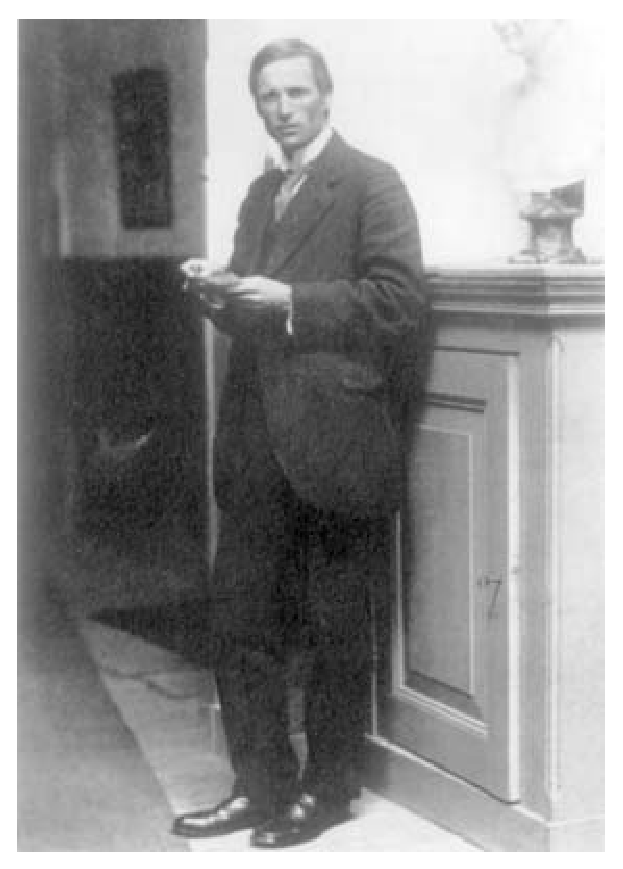
\includegraphics[height=6.0cm]{ambsthermopict/Brouwer.eps} 
} 
\caption{Cantor and Brouwer.}
\label{breakingwave2} 
\end{figure}





 








\fi  % --- end removed block (RNS as a Model of Physics) ---

\chapter{Cosmology: RNS with Gravitation}\label{ch:cosmology}

\small
\begin{quote} According to the \emph{Perfect Cosmological Principle}, 
the Universe on a large scale looks the same everywhere and at all times.
(Fred Hoyle)
\end{quote}
\begin{quote} The thermodynamic properties of self-gravitating
systems are still unclear...The tendency of increasing granularity with time
(in a self-gravitating system), so important to the structure and development 
of the Universe, seems to represent a fundamental principle. 
(Paul Davies \cite{davies})
\end{quote}
\begin{quote} 
GRAVITATION: The universal property of all material objects
to attract each other.\\
GRAVITON: A hypothetical particle which, when passing
to and fro in virtual form bewteen two masses, in large numbers,
is thought to mediate the gravitational attraction between them.
(Guillemin \cite{guillemin})
\end{quote}
\normalsize

\normalsize

\section{Euler's Equations with Gravitation}

The Euler equations including gravitational forces from the mass distribution
can be viewed as a basic (non-relativistic) \emph{cosmological model}.  
We thus consider an inviscid perfect gas 
enclosed in a volume $\Omega$ in $\bbR^3$ with boundary $\Gamma$
(or the whole of $\bbR^3$), over a time interval $I=(0,1]$, assuming 
that the gas is subject to a gravitational force $\nabla\varphi$, where
$\varphi$ is a \emph{gravitational potential} 
coupled (at each time instant) to the mass distribution $\rho$  
through Poisson's equation $\Delta\varphi =\rho$
with (for simplicity) $\varphi =0$ on $\Gamma$. This is a 
\emph{self-gravitating system} since the gravitational force depends
on the mass-distribution  

Replacing $\rho$ by $\Delta\varphi$, we are led to the following version
of Euler's equations with gravitation:  
Find $\hat u=(\varphi ,m,e)$ 
depending on $(x,t)\in Q\equiv \Omega\times I$ such that
\begin{equation}\label{eulergrav}
\begin{array}{rcl}
\Delta\dot\varphi +\nabla\cdot m &=&  0 \quad \mbox{in } Q, \\
\dot m +\nabla\cdot (mu) +\nabla p-\rho\nabla\varphi&=&  0 \quad \mbox{in } Q, \\
\dot e +\nabla\cdot (eu)+p\nabla\cdot u &=& 0  \quad \mbox{in } Q,\\ 
u\cdot n&=&0\quad \mbox{on } \Gamma\times I\\
\varphi &=&0\quad \mbox{on } \Gamma\times I\\
\hat u(\cdot ,0)&=&\hat u^0\quad \mbox{in } \Omega , 
\end{array} 
\end{equation}
where $u=\frac{m}{\Delta\varphi}$, 
$p=(\gamma -1)e$ with $\gamma >1$, and we normalize the gravitational
constant to unity.

\section{The Hen and the Egg}

An interesting aspect of this model with the gravitational
potential $\varphi$ as a primary variable and the mass distribution
$\rho$ as a derived quantity, is that it does not include
\emph{action at distance} in the same way as the conventional model
with $\varphi$ derived from $\rho$ through Poisson's equation 
$\Delta\varphi =\rho$. Instead we have to deal
with the new equation $\Delta\dot\varphi +\nabla\cdot m =0$,
still containing the Laplacian.

Considering the equation $\Delta\varphi =\rho$ as defining
$\varphi$ in terms of $\rho$ or vice versa, of course connects
to which comes first: the egg or the hen. 

Choosing (in an exam for example) 
to explain either how a hen can lay an egg
or how an egg can develop into a hen, you may go for the first
option as appearing to be (somewhat) simpler to deal with.
The idea would be that it would be advantageous to
choose the more complex object of the 
potential/hen rather than the simpler mass/egg, as 
the primary unknown which will come out by solving the equations,
(by some form of computation).
Thus the more complex object, the potential/hen will 
be ``created by computation'' in front of our eyes, thus relieving us
from \emph{explaining} how a mass/egg can create a potential/hen. 
But doing so we have to deal with 
the equation $\Delta\dot\varphi +\nabla\cdot m=0$
expressing ``mass conservation'' in a non-standard form,
which  admittedly seems to involve action at distance if we rewrite it in the form.
$\dot\varphi +(\Delta )^{-1}\nabla\cdot m=0$ for the purpose
of explicitly updating $\varphi$ by time-stepping. What can we do 
to allow time-stepping without inverting the Laplacian?

\section{Perturbed Mass Conservation} 

Well, we may consider
to perturb the equation for mass conservation
$\Delta\dot\varphi +\nabla\cdot m=0$ into: 
\[
\kappa\ddot\varphi -  \Delta\dot\varphi -\nabla\cdot m=0
\]
with $\kappa$ a small positive constant, now allowing time stepping
without inverting the Laplacian. Of course, you could regularize the
equation $\Delta\varphi =\rho$ similarly into  
$\kappa\dot\varphi -\Delta\varphi =\rho$ keeping mass conservation in the
standard form $\dot\rho +\nabla\cdot (\rho u)=0$. In any case,
(\ref{eulergrav}) with $\varphi$ instead of $\rho$ and a perturbed
equation for mass conservation, is a model without action at distance.


\section{Gravitons?}

Solving Poisson's equation $\Delta\varphi =\rho$
equation for the gravitational
potential $\varphi$ in terms of the density $\rho$, reflect that
(somehow) a mass distribution ``creates'' its own gravitational field
(seemingly infinitely fast). The physics of this creation of a hen out
of an egg in the form of
a gravitational potential/force from a mass distribution, is unknown: A
conjecture is that the gravitational field is 
established through an \emph{exchange} of certain hypothetical particles 
called \emph{``gravitons''}. But no gravitons have been detected despite
intense search.



The reverse question is how a hen can lay an egg 
or how a gravitational potential can ``create'' a mass.
A potential with a sharp peak of the form 
$\frac{1}{4\pi\vert x-\bar x\vert}$, would then represent a
unit mass at position $\bar x$.  
In this perspective a tendency of ``mass lumping'' from 
very small initial density
variations, is to be expected from the fact that application of the Laplacian
may enhances variations and thus create positive and negative peaks/masses
out of nothing, with masses of different equal signs attracting each other
and masses with different signs repelleing each other. Our Universe
with positive masses would thus have a twin Universe with negative masses.

In this model, it is thus the gravitational 
potential $\phi$, which is given initially
and which evolves in time (together with momentum and energy)
and from which the mass density $\rho$ is generated by $\Delta\phi =\rho$
in a local ``creation process''.
We here avoid action at distance and we also get a hint
to the possible nature of all the ``dark mass'' seemingly required to account 
for the observed gravitational forces on cosmic scales, as 
mollified potential peaks not strong enough to 
``create visible mass'', but yet having gradients and exerting
gravitational forces.

%The alternative model (\ref{cosmology2}) with $\delta >0$ is a wave equation 
%with finite speed of propagation depending on $\delta$. The proper choice
%of $\delta$ from physical point of view is unclear, while 
%we expect certain outputs to be insensitive to the choice of $\delta$.

\section{The 2nd Law with Gravitation}

The 2nd Law with gravitation takes the form
\begin{equation}
\dot K=W-D+ P,\quad \dot E=-W+D,\quad D>0,
\end{equation}
where 
\[
\begin{split}
P&=-\int_\Omega \rho\nabla\varphi\cdot u\, dx =+\int_\Omega \varphi\nabla\cdot m\, dx=-\int_\Omega\varphi\dot\rho\, dx= \dot\Phi,\\
\Phi &=-\frac{1}{2}\int_\Omega \varphi\Delta\varphi\,dx =\frac{1}{2}\int_\Omega\vert\nabla\varphi\vert^2\, dx.
\end{split}
\] 
By summation, we have
\[
\frac{d}{dt}(K+E -\Phi)=0
\]
stating that the total energy, the sum of
kinetic, heat and gravitational energy $K+E -\Phi$, is conserved.

\section{Irreversibility and Heat Death}

A natural scenario is to start with a hot compressed gas at rest, which is
let free to expand in a \emph{Big Bang} with $W-D-P>0$ setting the
gas in motion until $W-D-P<0$ and $K=0$, whereupon the gas
contracts by gravitation back to a hot compressed state in a \emph{Big Crunch}
allowing the process to start all over with a new Big Bang.

In each cycle of this process some kinetic energy would irreversibly
be transformed into heat energy, which ultimately could lead to 
a stationary state with $W=D$ and $P=0$, a \emph{heat death}. But the 
whole process may have many cycles....and so there may have been Worlds
and intelligent cultures including thermodynamics  
even before the Big Bang of the World we happen to live in...   

\section{A Self-Gravitating Gas in a Box}

To probe the thermodynamics of (\ref{eulergrav}) concretely we solve a
discrete form on a cubic grid filling a box $\Omega =[0,1]^3$, in conservation
form for the density $\rho$, the momentum $m=\rho u$ and the internal energy
density $e$, with the ideal-gas closure
\begin{equation}\label{closure}
p=(\gamma -1)e=\rho T,\qquad \gamma >1,
\end{equation}
so that $T=p/\rho$ is the temperature and $\gamma$ the adiabatic index. The
self-gravitation is supplied through the \emph{mean-subtracted} Poisson coupling
\begin{equation}\label{jeansswindle}
\Delta\varphi = G\,(\rho -\bar\rho ),\qquad
\bar\rho =\frac{1}{\vert\Omega\vert}\int_\Omega\rho\, dx,
\end{equation}
with $\varphi =0$ on $\Gamma$, where $G>0$ is the \emph{gravitational coupling}
(playing the role of $4\pi G_{\mathrm{Newton}}$) and $\bar\rho$ the mean density.

The subtraction of $\bar\rho$ is essential and is the classical
\emph{Jeans swindle}. A strictly uniform gas in a \emph{finite} box is not
force-free if $\rho$ itself sources $\varphi$: with $\varphi =0$ on $\Gamma$ the
solution of $\Delta\varphi =G\rho$ bulges in the interior, so a net inward force
develops everywhere and the whole box \emph{breathes} in and out --- an artifact
of the boundary rather than of any structure in the gas. Sourcing $\varphi$ from
the density \emph{contrast} $\rho -\bar\rho$ makes the uniform background exactly
force-free, so that only departures from uniformity gravitate. This is precisely
what one wants of a cosmological model: it is the \emph{granularity}, not the
mean, that drives the dynamics.

The model so written has exactly \emph{two} control parameters: the
gravitational coupling $G$ and the adiabatic index $\gamma$. Everything in the
competition between collapse and dispersal is decided by these two, as we now
show.

\section{Pressure versus Gravitation: the Jeans Criterion}

Linearize (\ref{eulergrav}), (\ref{closure}), (\ref{jeansswindle}) about a
uniform state $\rho =\bar\rho$, $u=0$, $T=\bar T$ at rest. Writing the density
perturbation as $\delta\rho$ and eliminating $m$ and $\varphi$ one obtains the
wave equation
\begin{equation}\label{waveeq}
\ddot{\delta\rho}=c_s^2\,\Delta(\delta\rho)+G\bar\rho\,\delta\rho,
\qquad c_s^2=\gamma\,\frac{\bar p}{\bar\rho}=\gamma\bar T,
\end{equation}
where $c_s$ is the adiabatic sound speed. For a plane wave
$\delta\rho\propto\exp(i(k\cdot x-\omega t))$ this gives the
\emph{Jeans dispersion relation}
\begin{equation}\label{dispersion}
\omega^2=c_s^2k^2-G\bar\rho=\gamma\bar T\,k^2-G\bar\rho .
\end{equation}
The first term, from pressure, is \emph{stabilizing} (it grows with $\gamma$);
the second, from gravitation, is \emph{destabilizing} (it grows with $G$). A
perturbation grows --- the gas \emph{collapses} --- precisely when
$\omega^2<0$, i.e.\ when
\begin{equation}\label{jeanscrit}
G\bar\rho>\gamma\bar T\,k^2
\qquad\Longleftrightarrow\qquad
\lambda>\lambda_J=2\pi\sqrt{\frac{\gamma\bar T}{G\bar\rho}}\, ,
\end{equation}
$\lambda_J$ being the \emph{Jeans length}. Below the Jeans length pressure wins
and the perturbation merely oscillates as a sound wave ($\omega^2>0$); above it
gravity wins and the perturbation grows.

The decisive observation is that the onset of collapse depends on $G$ and
$\gamma$ \emph{only through the ratio} $G/\gamma$: at a fixed scale $k$ and
fixed background $(\bar\rho ,\bar T)$, doubling the coupling $G$ has exactly the
same effect as halving the stiffness $\gamma$. The dimensionless number that
decides everything is
\begin{equation}\label{jeansnumber}
J=\frac{G\bar\rho}{\gamma\bar T\,k^2},
\qquad\text{collapse}\iff J>1 .
\end{equation}

In a box of side $L$ the longest available wavelength is $\lambda\approx L$, so
structure forms \emph{at all} only if $\lambda_J\lesssim L$, that is
\begin{equation}\label{boxthreshold}
G\gtrsim (2\pi)^2\,\frac{\gamma\bar T}{\bar\rho\,L^2}.
\end{equation}
For $\gamma =2$ and $\bar T=\bar\rho =L=1$ this requires $G\gtrsim 79$; for a
seed of size $\sim L/3$ the threshold is about nine times larger. Below it the
box is Jeans-stable at \emph{every} scale and any initial lump simply pulsates.
This is why a modest coupling produces only an oscillation and never a collapse:
$G$ has not been pushed past the Jeans threshold set by $\gamma$.

\section{Collapse to a Stable Configuration: the Role of $\gamma$}

The Jeans criterion (\ref{jeanscrit}) decides whether collapse \emph{begins}.
Whether the collapse \emph{ends} in a stable, finite lump --- rather than
running away to a singular spike --- is a separate question, and it is decided
by $\gamma$ \emph{alone}, independently of $G$.

Consider a self-gravitating polytropic cloud of fixed mass $M$ and radius $R$.
Under adiabatic compression $p\propto\rho^\gamma$, so the internal energy
density scales as $e\propto\rho^\gamma\propto R^{-3\gamma}$ and the total
internal (thermal) energy as
\[
U=\int_\Omega e\,dx \;\propto\; R^{-3\gamma}\cdot R^3 \;=\; R^{-3(\gamma -1)},
\]
while the gravitational self-energy scales as
\[
W \;\propto\; -\frac{GM^2}{R}\;\propto\; -R^{-1}.
\]
The total energy is therefore $E(R)=A\,R^{-3(\gamma -1)}-B\,R^{-1}$ with
$A,B>0$. As $R\to 0$ the thermal term dominates --- and hence $E$ possesses a
\emph{minimum} at a finite radius, a stable hydrostatic equilibrium --- if and
only if it stiffens faster than gravity, $3(\gamma -1)>1$, that is
\begin{equation}\label{fourthirds}
\boxed{\;\gamma>\tfrac43\;}
\end{equation}
the classical \emph{Chandrasekhar index}. The three regimes are:
\begin{itemize}
\item $\gamma>\tfrac43$: pressure wins under compression; collapse is
\emph{arrested} at a finite quiescent lump, possibly after damped oscillations.
\item $\gamma<\tfrac43$: gravity wins at every compression; collapse
\emph{runs away}, no equilibrium exists.
\item $\gamma=\tfrac43$: the marginal case (governing, e.g., white-dwarf
stability).
\end{itemize}
Thus the two parameters play complementary roles: $G$ (through (\ref{jeanscrit}))
selects \emph{which scales collapse and how fast}, while $\gamma$ (through
(\ref{fourthirds})) decides \emph{whether the collapse can be stopped}. To reach
a stable bound configuration one needs \emph{both} a coupling $G$ large enough
to cross the Jeans threshold \emph{and} a stiffness $\gamma>\tfrac43$ so that the
endpoint is an equilibrium rather than a singularity.

\section{Breathing, Sloshing and Virialization}

These two criteria account for the phenomenology seen in the simulations.

\emph{Breathing.} A uniform gas in which $\rho$ (rather than $\rho-\bar\rho$)
sources $\varphi$ is not in equilibrium in a finite box: it contracts toward the
centre, pressure builds, it rebounds, and the box breathes globally while its
density stays nearly uniform. The Jeans swindle (\ref{jeansswindle}) removes
this boundary artifact, leaving only the genuine gravitational response to
density contrast.

\emph{Sloshing.} A pair of overdensities below the Jeans threshold
($J<1$ at their separation) does not collapse but exchanges mass back and forth
quasi-periodically between the two centres. This is a \emph{virial oscillation}
in the double-well gravitational potential: gas falling toward one centre
overshoots on its pressure and inertia, sloshes to the other, and returns. With
$\gamma>\tfrac43$ and no dissipation the oscillation is undamped, kinetic and
gravitational energy being traded reversibly, $\dot K=P=\dot\Phi$, exactly as in
the energy balance of \S\,\textit{The 2nd Law with Gravitation}.

\emph{Virialization.} To settle into a quiescent lump the gas must \emph{shed}
its infall energy: a stable bound configuration requires dissipation $D>0$ to
convert the ordered kinetic energy of collapse into heat. The entropy so
produced is the irreversible price of structure formation --- the mechanism
behind Davies' ``increasing granularity'' (\S\,\textit{Cosmology}) and behind
the heat death of \S\,\textit{Irreversibility and Heat Death}. Gravitational
structure forms by the conversion, through $D$, of gravitational potential
energy first into bulk motion and then, irreversibly, into heat.

\begin{remark}
In the numerical model the closure is written as $p=\gamma_s\,e$, so that the
adiabatic index is $\gamma=1+\gamma_s$; the stability boundary (\ref{fourthirds})
then reads $\gamma_s>\tfrac13$, and the coupling $G$ is exactly the
$4\pi G_{\mathrm{Newton}}$ of (\ref{jeansswindle}). The two sliders $(G,\gamma_s)$
of the interactive model are precisely the two parameters $(G,\gamma)$ of the
analysis above.
\end{remark}

\section{RNS Simulations of a Self-Gravitating Gas}

We give below some results from RNS solutions of (\ref{eulergrav})
showing the development mass granularity from
uniform mass distributions under expansion.

\begin{figure}[bhpt] 
\centerline{ 
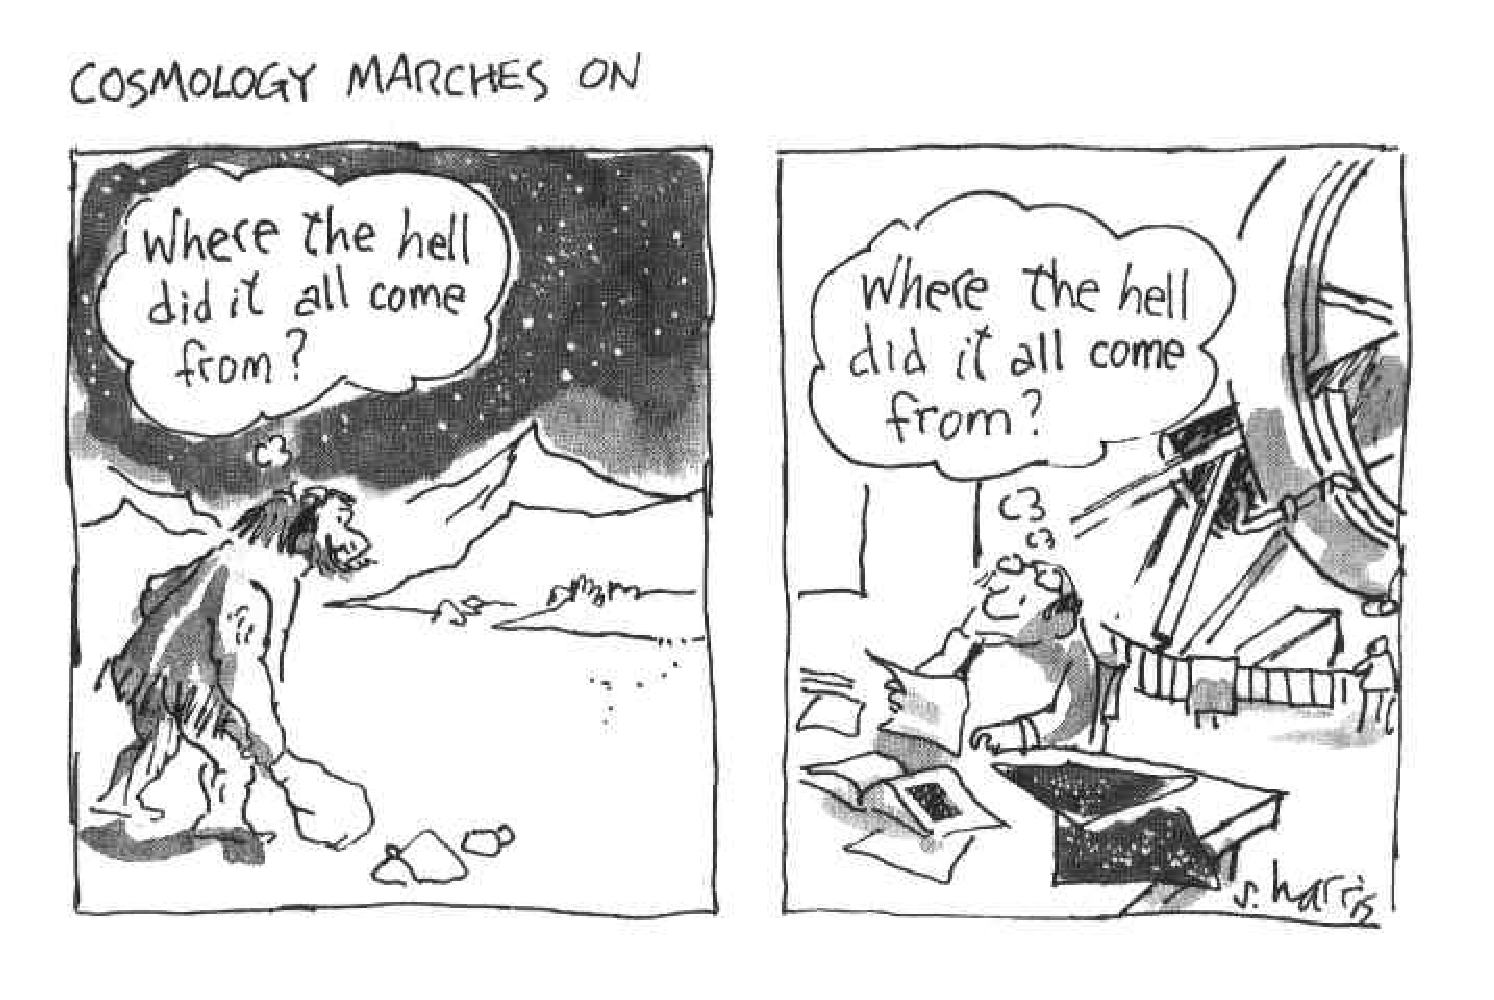
\includegraphics[height=8cm]{ambsthermopict/cosmology.eps} 
} 
\caption{Cosmology theories}
\label{cosmologytheory} 
\end{figure}



\begin{figure}[bhpt]
\centerline{
\includegraphics[height=8cm]{ambsthermopict/cosmology2.eps}
}
\caption{Big Bang expansion}
\label{bigbang2}
\end{figure}

\section{Browser-Runnable 3D RNS-Gravitation Simulator}\label{sec:cosmology_3d_gpu}

A WebGPU companion simulator
\texttt{cosmology\_3d\_gpu\_100.html} is shipped with the
RealMolecule repository
(\texttt{github.com/Claes542/RealMolecule}). It evolves the
self-gravitating RNS system (\ref{eulergrav}) on a $100\times100\times
100$ grid ($10^{6}$ cells) entirely in the browser, using WebGPU
compute shaders for the fluid update and a sub-stepped red-black
Gauss-Seidel relaxation for the Poisson equation $\Delta\varphi = G(\rho - \bar\rho)$.

\paragraph{Initial condition.}
A single Gaussian overdensity at the box centre, both denser and
hotter than the surrounding bath. This is the Big Bang initial
condition of Chapter~\ref{ch:bigbang}: a concentrated hot dense seed
in an otherwise uniform low-density background, with no initial
velocity. The Jeans-swindle source $G(\rho - \bar\rho)$ keeps the
background force-free so that only the density contrast pulls.

\paragraph{Live sliders.}
The simulator exposes the following live controls:
\begin{itemize}
\item \emph{$\gamma$} --- EOS parameter $p = \gamma e = \gamma\rho T$.
\item \emph{Gravity $G$} --- coupling strength.
\item \emph{Seed amp} --- peak overdensity (applied on Reset).
\item \emph{Shock visc $C$} --- shock-viscosity coefficient.
\item \emph{Art visc $\nu$} --- background artificial viscosity.
\item \emph{Seed every} --- particle-trace reset interval.
\item \emph{Trace speed} --- velocity magnification for particle advection.
\item \emph{Fluid substeps/frame} --- numerical resolution in time.
\item \emph{Poisson iters/fluid step} --- gravity convergence.
\end{itemize}

\paragraph{Recommended Big Bang $\to$ Big Crunch settings.}
For a single clean BB$\to$BC cycle followed by a stable virial state:
$G = 500$, seed amp $= 0.5$, $\nu = 1.0$, shock $C = 3.0$, $\gamma = 1$,
Poisson iters $= 10$ or higher for long-time stability.

\paragraph{Reading the display.}
\begin{itemize}
\item \emph{Red particle traces} on the mid-plane: persistent advection
of test particles, redrawn periodically (see \emph{seed every} slider).
During BB the traces radiate outward; during BC they sweep inward;
once virial equilibrium is reached they continue to circulate along
divergence-free streamlines, reflecting the fact that
$\partial_t\rho = 0$ does \emph{not} mean $u = 0$.
\item \emph{Blue polyline} --- density profile $\rho(x_1, x_2^{\mathrm{mid}}, x_3^{\mathrm{mid}})-1$ on the mid-line cross-cut, auto-scaled.
\item \emph{Green polyline} --- temperature profile $T-1$ on the same line.
\item \emph{Cyan polyline} --- gravitational potential $\varphi$ on the same line.
\item \emph{Diagnostic readout} --- peak values of $|\varphi|$, $|\rho-1|$, $|u|$, and simulation time.
\end{itemize}

The simulator is the working companion to the present chapter and
Chapter~\ref{ch:bigbang}: the reader can vary $G$ and the seed amplitude
to scan the Jeans-criterion threshold, watch the
expansion-cooling and compression-warming phases of one Big Bang
followed by one Big Crunch directly in the temperature line plot, and
verify that the cumulative dissipation $D = \int\!\int\mu|\nabla u|^2\,dx\,dt$
prevents the system from oscillating indefinitely.





\chapter{ThermoDynamics of Big Bang and Big Crunch}\label{ch:bigbang}

\small
\begin{quote}\itshape
The Big Bang is the simplest thermodynamic event in the universe.
A hot, dense, expanding fluid cools. The pressure-work term
$-\,p\,\nabla\!\cdot u$ of \S\ref{sec:expansion_cools} is positive, the
expansion is everywhere, and the cooling is universal.
\end{quote}
\normalsize

\section{Expansion Cools, at Cosmic Scale}

The thermodynamic content of the Big Bang follows directly from the
two primitives of Chapter~\ref{ch:entropy_turbulence}, applied to the
self-gravitating compressible fluid of
Chapter~\ref{ch:cosmology}. The early universe is a hot dense plasma
in which every comoving fluid element has positive divergence:
$\nabla\!\cdot u > 0$ everywhere, at every time. By the
expansion-cools primitive (\S\ref{sec:expansion_cools}), the
internal-energy equation gives
\[
  \dot e \;=\; -\,p\,\nabla\!\cdot u + \mu_{\mathrm{mom}}|\nabla u|^2
  \;<\; 0
\]
in regions where the pressure work dominates the dissipation, i.e.\
where the bulk expansion of the universe is the dominant dynamical
process. Internal energy decreases, temperature drops, and the
universe cools. There is no fine-tuning in this; it is the same
$-p\,\nabla\!\cdot u$ term that cools the gas in the left chamber of
Joule's experiment (Chapter~\ref{ch:joule}), now applied to a gas
whose container is the universe itself.

The cooling timeline is fixed once the equation of state and the
initial conditions are. The radiation-dominated era ($T \gg
10^4\,\mathrm{K}$, $\nabla\!\cdot u \propto t^{-1}$) cools as $T
\propto a^{-1}$ with $a \propto t^{1/2}$; the matter-dominated era
cools as $T \propto a^{-2}$ with $a \propto t^{2/3}$; and the
present-day cosmic microwave background sits at $T \approx 2.7\,\mathrm{K}$,
the remnant of the radiation field after $\sim 13.8$ billion years of
expansion-cooling. No part of this is statistical; all of it is the
expansion-cools primitive applied at cosmic scale and integrated over
cosmic time.

\section{The CMB as Blackbody Cutoff Signature}

The most direct experimental signature of the Big Bang ---  the
cosmic microwave background --- is the radiative half of the story.
At the recombination epoch ($z \approx 1100$, $T \approx 3000\,\mathrm{K}$)
the electrons and protons combined into neutral hydrogen, the
universe became transparent, and the radiation field decoupled from
the matter field. From that moment on, the radiation field expanded
with the universe at fixed photon number, with the spectrum
red-shifted as $\omega \to \omega/a$ and the temperature dropping as
$T \to T/a$. The Planck spectrum maintains its functional form under
this transformation --- a remarkable feature of the blackbody
spectrum, and a non-trivial test of the with-Dynamics reading of
Chapter~\ref{ch:blackbody}: the cutoff at $\omega \sim
k_{\mathrm{B}}T/\hbar$ rescales together with $T$, so a Planck
distribution at $T_{\mathrm{rec}} = 3000\,\mathrm{K}$ at recombination
becomes a Planck distribution at $T_{\mathrm{today}} = 2.7\,\mathrm{K}$
today, observed as the CMB.

The high-frequency tail of the early radiation field --- the part
that, before recombination, was being thermalised by the
free-electron bath at the blackbody cutoff --- has its present-day
counterpart in the small fraction of the CMB energy that even now
continues to be absorbed and re-emitted by intervening matter, with a
cumulative entropy production whose continuum-mechanics realisation
is the cosmological dissipation $D = \int\!\int
\mu_{\mathrm{mom}}|\nabla u|^2\,dx\,dt$ of the gravity-coupled RNS
flow.

\section{The Joule Pattern at Cosmic Scale}

The three-stage Joule pattern that organises this volume applies to
the Big Bang at cosmic scale:

\begin{enumerate}
\item \textbf{Internal energy reservoir.} The initial hot dense plasma
holds an enormous internal energy density. This is the cosmic
analogue of the high-pressure gas in Joule's left chamber.

\item \textbf{Conversion to bulk kinetic energy.} The Hubble expansion
converts internal energy into the bulk kinetic energy of the comoving
fluid through the pressure-work term, exactly as in Joule's free
expansion --- only with the geometry of an isotropic three-dimensional
expansion rather than a channel between two chambers.

\item \textbf{Dissipation into the bath.} The bulk kinetic energy is
in turn dissipated, at every scale at which structure forms, by the
turbulent and shock-front dynamics of the gravity-coupled RNS flow.
This dissipation is what allowed galaxies, stars, and planets to
condense out of an initially smooth distribution --- the
$D$-generating processes of the previous chapter, played out in the
cosmological setting.
\end{enumerate}

The asymmetry between the two halves of the Joule experiment is here
asymmetry between cosmic expansion (bulk, smooth, universal) and
structure formation (local, dissipative, gravitationally-driven). The
universe as a whole is in the expansion-cools half of the cycle. The
local condensations --- galaxy clusters, galaxies, stars, planets ---
are sites where the structure-formation half has run its
$D$-generating dynamics far enough to produce stable, locally bound
configurations of the kind discussed in Chapter~\ref{ch:cosmology}.

\section{Big Crunch: Compression Warms, at Cosmic Scale}

The hypothetical \emph{Big Crunch}, in which a closed universe whose
present expansion is eventually reversed by its own gravity collapses
back to a hot dense state, is the cosmic-scale realisation of the
compression-warms half of the primitive of
\S\ref{sec:expansion_cools}. The pressure-work term that drives the
universal cooling in the expansion-dominated era,
\[
  -\,p\,\nabla\!\cdot u,
\]
reverses sign once $\nabla\!\cdot u$ does. In a contracting universe
the pressure work is positive, internal energy is increasing, and the
universe \emph{warms}. The same mechanism that delivered the
present-day $2.7\,\mathrm{K}$ CMB by 13.8 billion years of
expansion-cooling would, run in reverse over the symmetric
timescale, deliver an arbitrarily hot final state by the same number
of e-foldings of compression-warming.

Big Bang and Big Crunch are therefore not two different physical
mechanisms but the two signs of the same one --- the cosmic-scale
$-p\,\nabla\!\cdot u$ term, with $\nabla\!\cdot u > 0$ in the
expansion era and $\nabla\!\cdot u < 0$ in the contraction era. The
companion \texttt{cosmology\_2d\_cpu.html} simulator can be run in
either mode by choice of initial conditions: with hot dense central
patch and zero initial velocity (Big Bang); or with initially cool
dispersed matter assembled under its own gravity into a single
collapsing mass (Big Crunch). The diagnostics readout shows the
expansion-cooling in the first case and the compression-warming in
the second.

A point worth noting: the irreversible dissipation $D \geq 0$ does
\emph{not} reverse sign with the expansion. Even in a contracting
universe, the local turbulent and shock-front processes that
generate $D$ continue to convert organised kinetic energy into heat.
The Big Crunch, in the with-Dynamics framework, is not a
time-reversal of the Big Bang --- it is the Big Bang's structural
mirror in the bulk pressure-work term, accompanied by the same
unidirectional irreversibility of $D$ in the small-scale dynamics.
What classical state-function thermodynamics would describe by a
``maximum entropy at the moment of maximum expansion'' the
with-Dynamics framework describes by: the integral $\int D\,dt$ over
the whole history continues to grow, even as the bulk pressure work
reverses direction.

\section{Is the Big Bang/Crunch Inherently 3D?}

The expansion-cools / compression-warms mechanism itself is
\emph{dimension-free}. The pressure-work term
$-\,p\,\nabla\!\cdot u$ is a continuum-mechanics object that lives
in any dimension $d$, with the divergence simply summing more terms:
$\nabla\!\cdot u = \sum_{i=1}^d \partial u_i/\partial x_i$. A 1D Big
Bang (a slab expanding along one axis), a 2D Big Bang (a sheet
expanding radially in a plane --- what
\texttt{cosmology\_2d\_cpu.html} simulates), and the 3D Big Bang all
obey the same primitive. The cumulative dissipation
$D = \int\!\int \mu_{\mathrm{mom}}|\nabla u|^2\,dx\,dt$ is also
dimension-free.

But the \emph{specific structure} of our observed universe is
3D-specific:

\begin{itemize}
\item \textbf{Gravity.} Newton's law in $d$ dimensions falls off as
$1/r^{d-2}$. In $d=1$ gravity grows linearly with distance
(collapse is inevitable, no structure formation regime); in $d=2$
it is logarithmic (marginal); only in $d=3$ does it fall off fast
enough to give the Jeans criterion that allows the bulk expansion
to coexist with local condensation into bound structures.

\item \textbf{Stable bound orbits.} Bertrand's theorem singles out
$d=3$ as the dimension in which closed bound orbits exist under an
inverse-square central force. 2D galaxies and stars would form
qualitatively differently; in $d \geq 4$ they would not form stable
bound orbits at all.

\item \textbf{Radiation density of states.} Photon modes per unit
frequency go as $\omega^{d-1}$. The CMB spectrum is a Planck
distribution with $\omega^3$ density of states; in 2D the
corresponding spectrum would have $\omega^1$ scaling, with a
different Stefan--Boltzmann constant and a different
expansion-cooling trajectory for the radiation temperature.

\item \textbf{Jeans criterion.} The condition for gravitational
collapse depends on dimension through both the gravitational
coupling and the pressure response. Only in $d=3$ does the
classical Jeans length come out at the scale that organises
structure formation as we observe it.
\end{itemize}

The 2D simulator \texttt{cosmology\_2d\_cpu.html} is therefore a
qualitative illustration: it captures the bulk pressure-work term
faithfully and demonstrates expansion-cooling and
compression-warming, but does not reproduce the $d=3$-specific
structure-formation regime.

\section{Computational Big Bang and Big Crunch}

For quantitatively faithful Big Bang / Big Crunch simulations the
3D companions are required. The repository ships two
WebGPU-accelerated 3D self-gravitating RNS simulators:

\begin{itemize}
\item \texttt{cosmology\_3d\_gpu\_100.html} --- $100 \times 100 \times
100$ grid ($10^6$ cells), suitable for desktop GPUs.
\item \texttt{cosmology\_3d\_gpu\_200.html} --- $200 \times 200 \times
200$ grid ($8 \times 10^6$ cells), suitable for high-end GPUs.
\end{itemize}

Both implement the same compressible-flow RNS apparatus coupled to a
Poisson-solved gravitational potential, with sliders for the central
patch density and temperature (Big Bang initial condition), for the
gravitational coupling $G$, and for the EOS parameter $\gamma$ that
sets the pressure response. The reader can observe the expansion-cools
phase, the formation of localised gravitational condensations, the
$D$-generating turbulent and shock dynamics that allow those
condensations to virialise into stable bound configurations, and ---
by choice of initial conditions and $G$ --- the compression-warming
of a Big-Crunch-like trajectory.

The Cosmology chapter (Ch.~\ref{ch:cosmology}) develops the
self-gravitating RNS apparatus and uses the simpler
\texttt{cosmology\_2d\_cpu.html} as its working example. The full 3D
companions are referenced there and used here for the explicitly
cosmological Big Bang / Big Crunch initial conditions of the present
chapter.

The cosmological extension of the framework therefore requires no new
physics beyond what Chapters~\ref{ch:entropy_turbulence},
\ref{ch:blackbody}, and~\ref{ch:cosmology} already establish. The
Big Bang, read in the with-Dynamics framework, is the universe as a
single instance of the same compressible-flow apparatus that
organises Joule, refrigerators, heat engines, chemical bonding, and
blackbody radiation. The 2nd Law of the universe is the inevitability
of its dissipation $D$, and the cosmological expansion-cools is the
inevitability of its pressure-work term.


\chapter{RNS with Chemical Reactions}\label{ch:reactive}

\small
\begin{quote}
To every action there is always opposed an equal reaction: or, 
the mutual actions of two bodies upon each other are always equal, 
and directed to contrary parts. (Newton's 3rd Law)
\end{quote}
\begin{quote}
President Bush gave his first-ever presidential radio address in both 
English and Spanish. Reaction was mixed, however, as people were trying 
to figure out which one was which. (Dennis Miller)
\end{quote}
\normalsize

\section{Reactive Euler Equations}

We now generalize the Euler equations (\ref{eulergen}) to
a \emph{mixture} of $N$ gas species, undergoing $M$
chemical reactions: We seek the
\emph{species densities} $\rho_1,...,\rho_N$, the \emph{mixture 
momentum} $m=\rho u$ with 
$u=(u_1,u_2,u_3)$ the \emph{mixture velocity} and $\rho =\sum_i\rho_i$
the \emph{mixture density}, and the \emph{mixture internal energy} $e$
satisfying
%and the \emph{total energy} $\epsilon$ as functions of
%$(x,t)\in \Omega\cup\Gamma\times [0,\hat t\, ]$, where $x=(x_1,x_2,x_3)$
%denotes the coordinates in $\bbR^3$ and $u_i$ is the velocity
%in the $x_i$-direction.  The Euler equations for 
%$\hat u\equiv (\rho, u, \epsilon)$ 
%read with $Q=\Omega\times I$ and $I=(0,\hat t\, ]$:   
\begin{equation}\label{eulerreact} 
\begin{array}{rcll} 
\dot\rho_i +\nabla\cdot (\rho_i u)&=& s_i,\quad  &\mbox{in }Q,\quad i=1,...,N,\\
\dot m+\nabla\cdot(mu)+ \nabla p &=&  f \quad &\mbox{in } Q, \\ 
 
\dot e +\nabla\cdot (eu)+p\nabla\cdot u&=& \sum_is_ir_i\quad &\mbox{in }Q,\\
  u\cdot n &=& 0   \qquad  &\mbox{on }  \Gamma\times I,\\                       
\hat u(\cdot ,0) &=&  \hat u^0\qquad &\mbox{in }  \Omega , 
\end{array} 
\end{equation}
where $s_i$ is the net reaction rate of species $i$ from all the
reactions, and we assume the following constitutive relations
\[
e=\sum_{i=1}^N\rho_ir_i+\rho\tau
\] 
with $\tau$ the \emph{mixture temperature} and $r_i$  
the \emph{heat of formation} of species $i$, together with a
\emph{mixture pressure} $p$ given as the sum of the partial pressures
from the different species: 
\[
p=C\tau \sum_i\frac{\rho_i}{W_i}.
\]
where $W_i$ is the molecular weight of species $i$ and $C$ a 
positive constant.
Evidently, we assume here that the species velocities are all equal to the
mixture velocity and that all species take on the mixture temperature.
%It is possible to generalize to individual species velocities,
%but the resulting model is complex. 
\section{Reaction Rates}
 
We assume that the reaction rate $s_i$ of species $i$ is given by an
\emph{Arrhenius law} of the form
%with $y_i=\rho_i/\rho$ is the 
%\emph{mass-fraction}, and
%$q=(q_j)$ is the mixture heat flux and $q^{D,i}$ is the diffusive 
%flux for species $i$,
%given by
%\[
%q=-\kappa \nabla (\rho c_vT),\qquad q^{D,i}=-D_i\nabla\rho_i,
%\]
%$\kappa\ge 0$ and $D_i\ge 0$ are diffusion coefficients, 
%and $c_v$ the heat capacity under constant volume.
%Further, the vector $S(u)=(s_1\,\cdot\cdot s_N,\, 0\,\cdot\cdot 0)$ models
%the chemical reactions and is typically given by
\[
s_i=W_i\sum_{k=1}^M (\nu^{\prime\prime}_{i,k}-\nu^{\prime}_{i,k})
B_kT^{\alpha_k}e^{-\frac{E_{\alpha ,k}}{RT}}\prod_{j=1}^N
(\frac{X_jp}{RT})^{\nu^{\prime}_{j,k}},
\]
where the $\nu$ are stochiometric coefficients, $R$ is the gas cosntant,
the $B_k$ are reaction
constants, $E_{\alpha ,k}$ is an activation energy, 
and
\[
X_i=\frac{\frac{\rho_i}{\rho W_i}}{\sum_j\frac{\rho_j}{\rho W_j}}
\]
is the mole fraction of species $i$.

\section{The 2nd Law for Reactive Euler}

The new 2nd Law takes the form:
%local form in this case, 
%choosing $\kappa =0$ and $D_i=0$ and 
\begin{equation}\label{2ndlaw3dlocal1react}
\dot K =W -D ,
\end{equation} 
\begin{equation}\label{2ndlaw3dlocal2react}
\dot E=-W+D +\sum_is_ir_i,
\end{equation}
%\begin{equation}\label{2ndlaw3dlocal3react}
%\dot T+w\cdot\nabla T+\frac{p\nabla\cdot w}{\rho} =\frac{\delta}{\rho}+
%\sum_ir_iy_i ,
%\end{equation}
%where 
%\[
%\delta =\lim_{\nu\rightarrow 0}\sum_{i=1}^3\nu\vert\nabla w_i\vert^2\ge 0,
%\]
%with $\delta >0$ for shocks/turbulence.
where $D\ge 0$ is the turbulent dissipation, and
\[
k=\frac{\rho\vert u\vert^2}{2},\quad K=\int_\Omega k\, dx,\quad E=\int_\Omega e\, dx,
\quad W=\int_\Omega p\nabla\cdot u\, dx.
\]
The 2nd Law shows irreversibility of turbulent mixing
and heating, while the chemical reactions as such, are reversible.

\section{Simulation of Combustion} 

\chapter{Loschmidt's and Gibbs' Paradoxes}

\small
\begin{quote}
How wonderful that we have met with a paradox.
Now we have some hope of making progress. \\(Nils Bohr)
\end{quote}
\begin{quote}
There is apparently a contradiction between the law of increasing entropy
and the principles of Newtonian mechanics, since the latter do not recognize 
any difference between past and future times. This is the so-called
reversibility paradox (Umkehreinwand) which was advanced as an objection
to Boltzmann's theory by Loschmidt 1876-77. (Translators foreword
to Lectures on Gas Theory by Boltzmann).
\end{quote}
\begin{quote}
Neither Herr Boltzmann nor Herr Planck has given 
a definition of $W$...
Usually $W$ is put equal to the number of complexions. In order
to calculate $W$, one needs a \emph{complete} (molecular-mechanical) theory
of the system under consideration. Therefore it is dubious whether the 
Boltzmann principle has any meaning without a 
\emph{complete} molecular-mechanical
theory or some other theory which describes the elementary processes (and such
a theory is missing). (Einstein)
\end{quote}
%\begin{quote}...the whole procedure was an act of despair because a
%theoretical interpretation had to be found at any price, no matter
%how high that might be... (Max Planck on the statistical mechanics basis of 
%his black-body radiation law)
%\end{quote}
%\begin{quote} Sommerfeld's very exhaustive discussion of Couette flow
%led to the conclusion that this type of flow remains stable for all
%viscosities. For a time, after this negative result had been obtained,
%it was thought that the method of small oscillations was unsuitable
%for the theoretical solution of the problem of transition to turbulence.
%It transpired later that this view was not justified, because Couette flow
%is a very special and restricted example. (Schlichting in Boundary Layer
%Theory, p 465, McGraw-Hill 1979)
%\end{quote}
\normalsize

\section{Scientific Paradoxes}
We now present new resolutions of \emph{Loschmidt's paradox}
on irreversibility in reversible Hamiltonian systems and 
\emph{Gibbs' paradox} on inextensivity of Boltzmann's entropy. 
We first give some give some general comments
on the role of paradoxes in science.
 
The above citation by the physicist Nils Bohr illustrates the  
role of a \emph{paradox} in the development of a physical theory, as a 
striking formulation of a contradiction within the theory,
or between a prediction of the theory and a factual observation.
Scientific progress can be made by showing that the contradiction is
only \emph{apparent}, thus improving the understanding of the meaning
of a theory remaining correct, or that the contradiction is \emph{real},
thus showing that the theory is not correct and thereby
opening for a new better theory to be developed. 
A theory predicting that an apple let free to fall, will stay where 
it is, will be contradicted by Newton's observation that the apple 
falls to the ground, and thus will have to be abandoned. 

The first known paradoxes were formulated by Zeno of Elea (490-430 BC) 
on the (still) puzzling nature of motion: Zeno asked e.g. how it can be that
a flying arrow, which at each instant looks just the same as a 
motionless arrow,
can be moving?
Modern physics harbors 
many unresolved paradoxes including the wave-particle duality of 
quantum mechanics and time dilation of special relativity.

Since an unresolved paradox is a deadly threat to a theory,
it has to be resolved by showing that the contradiction is only
apparent and not real, ``at any price, no matter
how high that might be...'' from the above citation of
the famous physicist Max Planck facing in 1900 the
paradox of the ultra-violet catastrophy in the classical theory
of black-body radiation.   

If a paradox
cannot be resolved by showing that the contradiction is only apparent
and not real,
it can be \emph{covered up} by presenting new
information. When asked where the tortoises can be seen,
which according to a certain (ancient) theory support the Earth,
the cover up would be to claim that they are invisible (but still there).   

In Loschmidt's paradox formulated in 1876 \cite{loschmidt},
mathematics of Hamiltonian systems (with zero viscosity)
predicts that time reversal and a perpetuum mobile is possible. 
But everybody (except possibly a physics specialist) knows that time is 
always moving forward and that a
perpetuum mobile is impossible, even though ultimately the World
is based on Hamiltonian (quantum) mechanics.

In Gibbs' paradox formulated in 1875, statistical mechanics predicts
that removing a membrane separating two volumes of equal gases at rest
in the same state (same density, temperature and pressure), will result in a 
significant increase of entropy. But everybody 
(except a statistical mechanics specialist) understands 
that removing (or inserting) a membrane in such a situation changes nothing.

\section{Cover Up} 
The cover up of Loschmidt's paradox by Boltzmann \cite{boltzmann}
is to introduce statistical mechanics
based on microscopic games of roulette. 
Statistical mechanics poses difficulties of
\emph{falsification} required by Popper in a scientific
theory, since
the validity of Boltzmann's basic microscopic assumption of 
statistical independence in a gas with each mole consisting of 
$6\cdot 10^{23}$ molecules,
% or 
%that electron positions have a probability distribution satisfying
%Schr\"odinger's equation, 
seems to be beyond the possibility of any kind of conceivable 
experiment or mathematics; 
only indirect evidence in the form of macroscopic observations seem to be 
possible, which is far from enough. In fact, it is known that Boltzmann's assumption
can only be (nearly) true in the very special case of a very dilute gas 
with rare collisions, and the derivation of Boltzmann equations
for more general situations seems to pose unsurmountable
problems.


The cover up of Gibbs' paradox by Gibbs' himself \cite{gibbs},
 is to change the counting of
microstates underlying Boltzmann's definition of entropy in 
statistical mechanics,
to give no change of entropy for equal gases, but retaining
a substantial entropy change as soon as the two gases differ 
slightly. We will below argue that such a discontinuous
change is not scientifically convincing, and present a different 
resolution based on computational turbulence avoiding tricky statistics.




\section{Resolution of Loschmidt's Paradox}

We have seen that the Euler equations are formally reversible
but in reality are irreversible, because pointwise solutions
to the Euler equations are non-existing. 
The irreversiblity arises because pointwise
conservation of momentum is impossible to achieve, while
the flow cannot cease to exist. The only way out is to
violate momentum balance and pay a penalty in the form
of turbulent dissipation with an irreversible transfer from kinetic 
to heat energy. 

In other words, pointwsie solutions of the Euler equations would have been 
reversible had they only existed, but they do not exist, 
and the weak dissipative solutions which do exist are irreversible
and thus define an Arrow of time.

More generally, Hamiltonian systems sufficiently complex to allow 
turbulence, have an Arrow of time defined without any reference to a 
concepts of entropy and statistical mechanics.







\section{Gibbs' Paradox}

On Boltzmann's tombstone the famous formula  
\begin{equation}\label{klogw}
S=k\log(W)
\end{equation}
 is engraved,
where $k$ is Boltzmann's constant 
($k\approx 10^{-23}$ joules/kelvin) and $W$ denotes the
probability of a certain state representing the number
of ''complexions'' or ``microstates'' corresponding to a ``macrostate''. 
Increasing entropy would then 
reflect that Nature would tend to move from less probable to more
probable states or towards states with more complexions. However,
the crucial questions \emph{why} and \emph{how} Nature would seek to always
increase entropy, was left without any answer. 

The definition $S=k\log(W)$ is different from
the classical expression $S=S=\log{\tau\rho^{-\gamma}}=\log(\tau V^\gamma )$
%=\log(p\rho^{-\gamma})$
derived above, which illustrates some of confusion surrounding
the classical concept of entropy 
in classical thermodynamics.

Boltzmann's statistical mechanics poses serious 
difficulties from scientific point of view and paradoxes line up. 
One of them is \emph{Gibbs' paradox} \cite{gibbs} illustrating the
difficulty of defining entropy by counting micro-states:
Consider a volume $V$ divided by a membrane into two equal volumes
$V/2$ filled with two different types of gas 
at rest with the same density and temperature.
Remove the membrane and let both gases expand to the 
double volume and come to rest in a mixed state. 
Gibbs recalls that according to Boltzmann the entropy 
of each gas would then increase by the factor 
$\gamma (\log(V)-\log(V/2))=\gamma \log(2)$, 
since for constant temperature $S=\gamma\log(V)$ with $V$ the volume of the
gas. The entropy of the system would then also increase by 
a $\gamma \log(2)$ factor.


Gibbs then compares with the case with the gases being of the same
type in which case removal of a membrane 
would change nothing and in particular the entropy should 
not change, in contrast to the above case.
In other words, the entropy should be \emph{extensive} 
in the sense that the entropy of a gas over a volume $V$ 
should be equal to the sum of the entropies over two volumes $V/2$. 
To achieve this, Gibbs suggested to change
the counting of microstates in the case of
equal gases, taking into account permutations of equal molecules,
but was then faced with a paradoxical discontinuos behavior 
of the entropy: No change 
for the same type of gas, and a $\log(2)$ change 
as soon as the types of gas differ only the slightest. 


\section{New Resolution of Gibbs'Paradox}

With our experience from the Joule-Thomson experiment, we can easily
resolve this paradox. It suffices
to note that an initial pressure difference resulting
from different state equations for two types of gas in the two
volumes, would drive a process towards equal pressure in 
the full volume, with the associated turbulent dissipation
(entropy production) being small if the initial pressure difference is small,
that is, if the type of gas is nearly the same.
In particular, for equal gases nothing would happen and 
there would be no sudden entropy jump under a slight change of gas, 
as in Gibbs' resolution by recounting microstates. 

We understand that the Gibbs'paradox results from Boltzmann's 
idea to define entropy by counting microstates, and thus 
is (one of many) indications that statistical mechanics creates more
problems than it solves, and from scientific point of view
therefore is questionable.    
 
 
  


%You might say: What you cannot know of, you don't have to worry about,
%in a travesty of Wittgenstein.


\begin{figure}[bhpt] 
\centerline{ 
%\includegraphics[height=6.0cm]{theoryoftimepict/boltzmann.eps} 
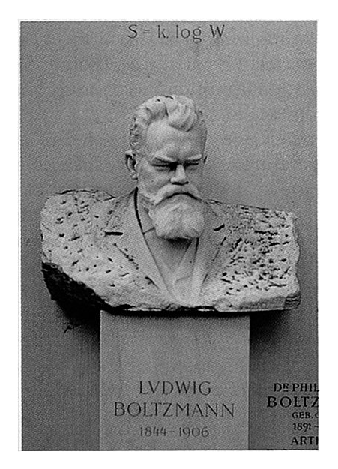
\includegraphics[height=14.0cm]{ambsthermopict/boltztombstone.eps} 
} 
\caption{Boltzmann's tombstone with $S=k\log(W)$.}
\label{breakingwave2} 
\end{figure}


\iffalse  % --- moved to Appendix (chapters/move_appendix_burgers.tex) at end of book ---
\part{Model Analysis}
 
\chapter{Burgers Equation}
\small
%\begin{quote}
%I feel sure that you do not understand how I came by
%my lonely ways. (Einstein about the statistical
%interpretation of quantum mechanics)
%\end{quote}
\begin{quote}
Some physicists. among them myself, cannot believe that we must abandon,
actually and forever, the idea of direct representation of physical reality
in space and time; or that we must accept then the view that events in nature
are analogous to a game of chance. (Einstein 1954)
\end{quote}

%\begin{quote}If God has made the world a perfect mechanism, He has at
%least conceded so much to our imperfect intellects that in order to
%predict little parts of it, we need not solve inumerable differential
%equations, but can use dice with fair success. (Born, on Quantum Physics)
%\end{quote}

\normalsize

\section{A Model of the Euler Equations}

As an instructive model of the 
Euler equations exhibiting basic aspects of
\emph{shock waves} and \emph{rarefaction waves}, 
we consider the following \emph{scalar conservation law}, referred to
as \emph{Burgers equation}:
Find the scalar function $u=u(x,t)$ such that
\begin{equation}\label{burgers}
\begin{array}{rcl}
\dot u +(f(u))^\prime &=&  0\quad\mbox{in }Q, \\
u(\cdot ,0)  &=&  u^0,
\end{array}
\end{equation}
where $f(u)=u^2/2$, $Q\equiv \bbR\times I$ with $I=(0,T]$,  
and we assume that the initial data 
$u^0(x)$ vanishes for large $\vert x\vert$.
%(which implies that $u(t,x)$ does the same for $t\in I$).
 
Burgers equation takes the pointwise form 
$\dot u+uu^\prime=0$ for a differentiable  pointwise solution $u$, which  
expresses that $u(x,t)$ is constant with values $u^0(\bar x)$
along straight lines $x=st+\bar x$ with slope $s=u^0(\bar x))$,
that is, along \emph{characteristics} defined by $\frac{dx}{dt}=u(x,t)$
with $x(0)=\bar x$. 

If $u^0(x)$ is increasing with increasing $x$ and is smooth, 
then there is a pointwise solution $u(t,x)$ for all time given by
the simple recipe 
\begin{equation}\label{uxu0}
u(x,t)=u^0(\bar x)\quad\mbox{for }
x=u^0(\bar x)t+\bar x.
\end{equation}
However, if the initial data $u^0(x)$ somewhere is
strictly decreasing, which of course will always be the case if 
$u^0(x)$ vanishes for large $\vert x\vert$, then characteristics will 
cross in finite time with different values and the solution 
formula gives conflicting function values, which can be 
interpreted as \emph{breakdown} of the pointwise solution. 
The result is 
that there is no differentiable function $u(x,t)$ satisfying
Burger's equation $\dot u+uu^\prime =0$ pointwise. 
We shall see
that this corresponds to the occurence of \emph{shocks}, 
which are represented by \emph{discontinuous} functions,
which satisfy the differential equation in a weak sense,
and in a pointwise sense only away from discontinuities
or jumps. 


What to do with an equation without pointwise solution? 
Of course, we regularize and consider instead the 
\emph{viscous/regularized Burgers equation}:
\begin{equation}\label{burgersreg}
\begin{array}{rcl}
\dot u +uu^\prime  -\nu u^{\prime\prime}&=&  0\quad \mbox{in }Q,\\
u(\cdot ,0)  &=&  u^0,
\end{array}
\end{equation} 
with $\nu >0$ a small viscosity. This problem can be solved
uniquely in a pointwise sense for all initial data, 
and as above the solution can be viewed as an approximate weak
solution to the original inviscid Burgers equation satisfying a 2nd
Law of the form
\begin{equation}\label{2ndlawBurgers}
\dot K(u;t)=-D_\nu (u;t)\quad\mbox{for }t\in I,
\end{equation}
where
\begin{equation}\label{KD}
\quad K(u;t)=\int_\bbR \frac{u(x,t)^2}{2}\, dx,\quad
D_\nu (u;t)=\int_\bbR\nu (u^\prime (x,t))^2\, dx.
\end{equation} 
The 2nd Law follows by multiplication of the viscous
Burgers' equation by $u$ and integration (by parts) with respect to $x$.


To give a perspective we now briefly recall the  
basics of the mathematical theory for conservation laws developed
in the 1950s motivated by the Euler equations of compressible
flow, in the model setting of Burgers equation. The basic idea is
to introduce the concept of \emph{weak solution} allowing discontinuous
solutions, and complement by a 2nd Law.  We shall see that the 2nd Law
singles out \emph{physical shocks}, which are discontinuous
weak solutions satisfying the 2nd Law, from \emph{non-physical shocks}
which are discontinuous weak solutions violating the 2nd Law.

We also present an alternative approach 
to single out physical shocks based on a stability analysis showing that a
a physical shock is stable and represents a
an observable physical phenomenon 
(like the ``bang'' from a supersonic airplane), 
while a non-physical shock is unstable and thus does not represent
any observable physical phenomenon.


%Before presenting the mathematicians solution we recall the basics:
%We thus a simple equation $\dot u+uu^\prime =0$ 
%which in general 
%\emph{has no pointwise solution}
%because of the inevitable occurence of shocks as soon as the initial
%data is decreasing. Similarly, the Euler equations 
%have no pointwise 
%solutions (except trivial solutions with constant velocity) because
%of the necessary appearnce of turbulence/shocks.

Burgers equation is formally reversible: If $u(x,t)$ is a 
pointwise solution in forward time on $[0,T]$, 
so is $-u(x,T-t)$ in reverse time. Burgers equation 
thus is formally reversible system, but in reality is irreversible, 
as a consequence of the non-existence of stable pointwise solutions. 
We thus use Burgers equation to illustrate that a World governed 
by the formally reversible Euler equations, is an irreversible
World, that is a world with an Arrow of time.




\section{Weak Solutions} 

A possibly
discontinuous function $u(x,t)$ is said to be a \emph{weak
solution to Burgers' 
equation} if 
\begin{equation}\label{burgersweak}\int_{\bbR\times\bbR_+} (-u\dot\varphi -f(u)\varphi^\prime )dx\, dt-
\int_\bbR u^0(x)\varphi (x,0)\, dx =0
\end{equation}
for all differentiable test functions $\varphi$ such that
$\varphi (x,t)$ vanishes for large $(x,t)$, assuming here
$I=(0,\infty )$.
%in $H^1(Q)$, where $Q=\bbR\times [0,T)$. 
This equation is obtained from (\ref{burgers}) by multiplication by
$\phi$ and integration by parts, shifting the derivatives
onto $\varphi$, thus allowing $u$ to be discontinuous. 

%A shock solution is thus 
%a weak solution but not a pointwise (strong) solution, since
%the differential equation is not defined at the point of the shock
%discontinuity. 



\section{The Rankine-Huginiot Condition}

A discontinuous function $u(x,t)$ defined by $u(x,t)=u_+$ if $x>st$ and 
$u(x,t)=u_-$ if $x<st$, where  $u_+$ and $u_-$ are two constant
states and $s$ is a constant, corresponding to a discontinuity 
propagating with speed $s$, is a weak solution
to Burgers' equation if the shock speed satisfies the 
\emph{Rankine-Hugoniot condition}
\begin{equation}\label{rh}
s=\frac{[f(u)]}{[u]},
\end{equation}
where $[u]=u_+-u_-$ and $[f(u)]=f(u_+ )-f(u_- )$. With $f(u)=u^2/2$
as in Burgers' equation, we have 
\begin{equation}\label{rhburgers}
s=(u_++u_-)/2.
\end{equation}
The Rankine-Hugoniot condition expresses the conservation law
(Burgers' equation)
in weak form for a piecewise constant discontinuous solution candidate $u$.


\section{Rarefaction wave}

The solution to Burgers equation with the \emph{increasing} 
discontinuous initial data $u^0(x)=0$ for $x<0$, and $u^0(x)=1$ for
$x>0$, is a \emph{rarefaction wave}
given by  
\begin{equation}\label{rarefaction}
\begin{array}{rcl}
u(x,t)&=& 0 \quad\mbox{for}\quad x<0,\\
u(x,t)&=& \frac{x}{t} \quad\mbox{for}\quad 0\le \frac{x}{t}\le 1,\\ 
u(x,t)&=& 1\quad\mbox{for}\quad 1< \frac{x}{t}.
\end{array}
\end{equation}
This is a continuous function for $t>0$
which satisfies (\ref{burgers}) pointwise
for $t>0$  off the lines $x=0$ and $x=t$ and can be viewed as
a pointwise solution (since it is continuous and piecewise
differentiable).
In a rarefaction wave, an
initial discontinuity separating two constant states develops into a 
continuous linear transition 
from one state to the other of width $t$ in space, 
corresponding to ``fan-like'' level curves in space-time as shown in
Fig. \ref{rarefactionfig}.
\begin{figure}[bhpt]
\begin{center}
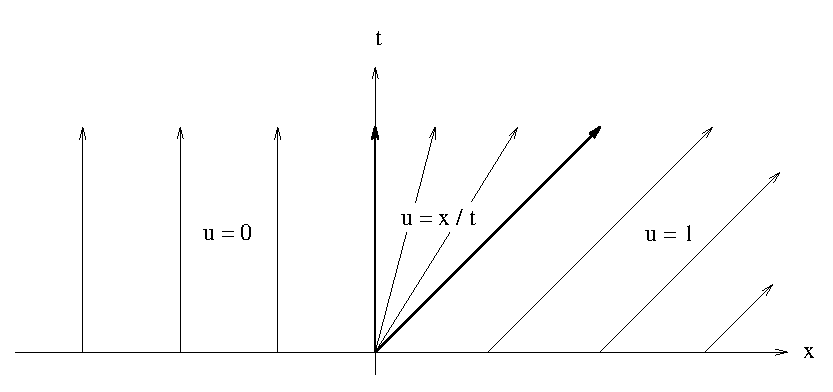
\includegraphics[height=3.3cm]{ambsthermopict/figRAchars.eps}
\caption{Characteristics of a rarefaction wave.}
\label{rarefactionfig}
\end{center}
\end{figure}
%\begin{figure}[bhpt]
%\begin{center}
%
\includegraphics[height=3.3cm]{figSHchars.eps}
%\caption{Characteristics of a shock}
%\label{shock}
%\end{center}
%\end{figure}






\section{Shock}

The solution with decreasing discontinuous initial data 
$u^0(x)=1$ for $x<0$, and $u^0(x)=0$ for
$x>0$, is a discontinuous \emph{shock wave} moving with speed $\frac{1}{2}$:
\begin{equation}\label{shock}
\begin{array}{rcl}
u(x,t)&=& 1 \quad\mbox{for}\quad x<\frac{t}{2},\\
u(x,t)&=& 0 \quad\mbox{for}\quad x>\frac{t}{2},  
\end{array}
\end{equation}
as shown in Fig \ref{shockfig}. We shall motivate that this is a 
\emph{physical shock}
satifying a 2nd Law.
\begin{figure}[bhpt]
\begin{center}
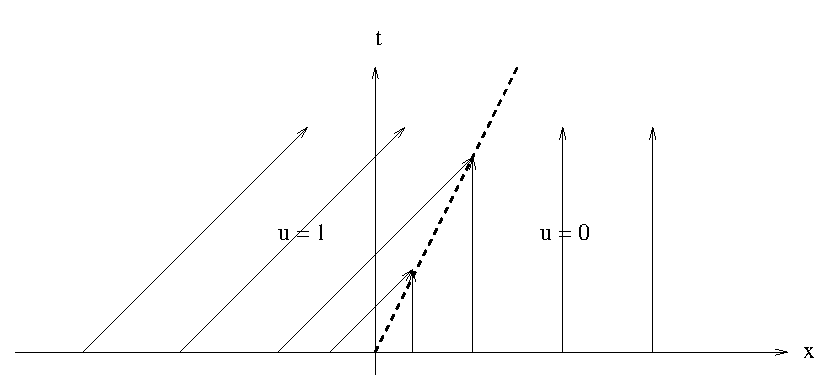
\includegraphics[height=3.3cm]{ambsthermopict/figSHchars.eps}
\caption{Characteristics of a shock}
\label{shockfig}
\end{center}
\end{figure}



\section{Weak solutions may be non-unique}

The rarefaction wave initial data 
$u^0(x)=0$ for $x<0$ and $u^0(x)=1$ for $x>0$, also admits
the alternative discontinuous weak solution 
\begin{equation}\label{unphyssol}
\begin{array}{rcl}
u(x,t)&=& 0 \quad\mbox{for}\quad x<\frac{t}{2},\\
u(x,t)&=& 1 \quad\mbox{for}\quad x>\frac{t}{2}, 
\end{array}
\end{equation}
corresponding to a discontinuity $\{x,t):x=st\}$ moving with speed
$s=\frac{1}{2}$. This solution is obviously
different from the rarefaction wave solution
(\ref{rarefaction}), which since it is a pointwise solution, also 
is a weak solution. Thus, we have in this case two different weak solutions, 
and thus we have an example of \emph{non-uniqueness of weak solutions.}
We shall see that the discontinuos solution (\ref{unphyssol}) 
violates the 2nd Law and thus is a \emph{non-physical shock solution}.
The physical solution in this case is the rarefaction wave
(which satisfies the 2nd Law with equality).



\section{The 2nd Law for Burgers Equation}

%The entropy inequalities are related to the Second Law of Thermodynamics
%stating that in a closed physical system, the entropy cannot
%decrease. Intuitively, the physical concept of ``entropy'' is related
%to ``disorder'' or ``loss of information'' and thus the  
%The Second Law states that disorder cannot decrease.
%To see how the Second Law in this form applies to the shock wave case above, 
%we note that the characteristics in this case ``converge into'' 
%the shock, which may be viewed as a ``loss of information'', or increase of entropy, 
%which is physically admissible.  On the other hand, for
%the unphysical solution (\ref{unphyssol}), the characteristics
%seem to ``emerge from'' the discontinuity, which may be viewed as
%some kind of ``creation of information'', which 
%would contradict the Second Law.
%Thus, in brief we may say that a discontinuous weak solution with
%the characteristics converging into the discontinuity, is a physical solution
%while it is unphysical if the characteristics are 
%divering out from the discontinuity.

We now check if (\ref{unphyssol}) satisfies the appropriate 
form of the 2nd Law (\ref{2ndlawBurgers})  
restricting space to $-1\le x\le 1$ and time to $0\le t\le 1$ assuming
the boundary conditions $u(-1,t)=0$ and $u(1,t)=1$. In this setting,
we obtain by multiplication of the viscous Burgers equation with $u$
and integrating by parts and using the sign of the viscous
term, the following form of the 2nd Law
\begin{equation}\label{2ndlawBurgers1}
-D_\nu (u;t)=  \dot K(u;t)+\int_{-1}^1(\frac{u^3}{3})^\prime =\dot K(u;t)+\frac{1}{3}
\end{equation} 
But for (\ref{unphyssol}) we have 
$\dot K=-\frac{1}{2}\frac{d}{dt}\frac{t}{2}=-\frac{1}{4}$, which
violates (\ref{2ndlawBurgers1}). 

Changing to the boundary conditions to $u(-1,t)=1$ and $u(1,t)=0$,
the 2nd Law changes to 
\begin{equation}\label{2ndlawBurgers2}
-D_\nu (u;t)= \dot K(u;t)+\int_{-1}^1(\frac{u^3}{3})^\prime =\dot K(u,t)-\frac{1}{3},
\end{equation} 
which is satisfied by (\ref{shock}) since now
$\dot K=\frac{1}{2}\frac{d}{dt}\frac{t}{2}=\frac{1}{4}<\frac{1}{3}$.

We conclude that a  discontinuous function $u(x,t)$ with the constant
states $u_-$ for $x<st$ and $u_+$ for $x>st$ corresponds
to a physical shock solution with shock speed $(u_-+u_+)/2$
if $u_-> u_+$, and to a non-physical 
shock if $u_-<u_+$.

We furher see that a shock dissipates substantial
kinetic energy into heat since for a viscous profile of width
$\nu$ joining two states $u_-$ and $u_+$   
\begin{equation}\label{Djump}
D_\nu (u;t)\equiv \int_\bbR\nu (u^\prime )^2\, dx\approx (u_--u_+)^2
\end{equation}
for small $\nu$.


\section{Burning Books}

The 2nd Law states that the characteristics of 
a physical shock  ``converge into'' the shock, corresponding
to $u_->u_+$. For the unphysical shock solutin
corresponding to the rarefaction
initial data with $u_-<u_+$, the characteristics
appear to ``emerge from'' the discontinuity. The
2nd Law thus allows information (features of the solution) to 
be ``destroyed'' (in a shock with converging characteristics), 
but not ``created out of nothing'' 
(in an unphysical rarefaction with diverging characteristics).
This connects to the essence of irreversibility: Burning books
can readily be done without any sophistication, while recovering the
original text from the ashes is impossible.  

\section{Stability of a Rarefaction Wave}

We shall now see that the 2nd Law can be replaced by a stability analysis
in its main mission to distingush physical shocks from unphysical shocks.
This reflects the fact that a stable process can be physically realized 
and observed, while an unstable process will have no permanence and
thus will be very difficult (or impossible) to realize.

The stability of a solution $u(x,t)$ is governed 
by the linearized equation 
\begin{equation}\label{linburgers}
\dot w+(uw)^\prime =0\quad\mbox{in }\bbR\times\bbR_+
\end{equation}
where $w$ represents a (small) perturbation (tending to zero for $\vert x\vert$
tending to infinity), and the solution $u$ acts as a 
given coefficient. The growth properties of the solution
$w$ of the linearized equation determines the stability:
If $w$ grows quickly in time, then the solution $u$ is unstable,
and if $w$ stays bounded, then $u$ is stable. Of course, stability
connects to finite precision: the level of the perturbation 
represents the precision.

We first consider the case of
a rarefaction wave given by (\ref{rarefaction}). Multiplying by $w$ and
integrating in space, we obtain by a simple computation using the fact
that $u^\prime (x,t)=1/t$ for $0\le x\le t$ and $u^\prime (x,t)=0$ else,
\[
\frac{d}{dt}\int_\bbR w^2(x,t)\, dx+
\int_0^t w^2(x,t)\frac{1}{t}\, dx =0,\quad\mbox{for }t>0,
\]
from which follows that
\begin{equation}\label{stabrarefaction}
\int_\bbR w^2(x,t)\, dx\le \int_\bbR w^2(x,0)\, dx\quad\mbox{for }t>0.
\end{equation}
This inequality shows that the $L_2$-norm in space
of a perturbation from initial data does not grow with time, 
which proves stability 
of a rarefaction wave. Note that this
argument builds on the fact that the rarefaction wave $u(x,t)$ is increasing in $x$ so that $u^\prime$ is
non-negative.

\section{Stability of Shock}

The stability proof used above to prove stability of a rarefaction
wave, does not work the same way for a shock, since in this case
$u(x,t)$ is decreasing with $x$. In fact a shock does not satisfy an
$L_2$ stability estimate of the form (\ref{stabrarefaction}). However,
one can prove instead an $L_1$-bound of the form
\begin{equation}\label{stabshock}
\int_\bbR \vert w(x,t)\vert\, dx\le \int_\bbR \vert w(x,0)\vert
\, dx\quad\mbox{for }t>0.
\end{equation}
This follows by multiplying (\ref{linburgers}) by $sgn (w)=+1$ if $w>0$ 
and $-1$ if $w<0$, to get by integration by parts:
\begin{equation}\label{linburgersL1}
\frac{d}{dt}
\int_\bbR\vert w(x,t)\vert\, dx +(u_--u_+)\vert w(\frac{t}{2},t)\vert =0,
\end{equation}
and using the fact that for a shock $u_+<u_-$.
Moreover, we will below with a different type of stability estimate
show that a shock is stable from computational RNS point of view, 
Thus, a shock is a stable phenomenon from both physical and computational
point of view.

%In one space dimension, shocks exist as piecewise constant
%(discontinuous) solutions, while in three space dimensions
%shocks in general generate turbulence. We present evidence in Vol 5.   

\section{Instability of Non-Physical Shock}

We saw above that the rarefaction wave solution is stable, and we now
study the stability of the alternative weak solution (\ref{unphyssol}).
By the same argument as used to prove (\ref{linburgersL1}) we obtain
\begin{equation}\label{linburgersL1unstable}
\frac{d}{dt}\int_\bbR\vert w(x,t)\vert\, dx =(u_+-u_-)\vert w(\frac{t}{2},t)\vert , 
\end{equation}
where now $u_+>u_-$. In this case, $\int_\bbR\vert w(x,t)\vert\, dx$
can grow arbitrarily fast, since the positive right hand side
in (\ref{linburgersL1unstable}) in no way can
be controled by the left hand side. We thus conclude that an 
unphysical shock is unstable.

\section{2nd Law $=$ Stability $+$ Finite Precision}
We thus have two methods
to single out physical shocks, one based on stability,
and the other based on the 2nd Law. This shows that ultimately the 2nd Law
expresses a stability condition, reflecting that Nature only can realize
phenomena which are properly stable, in its analog finite precision
computation. We thus may view the 2nd Law to express 
a combination of stability and finite precision.   


\section{A Traffic Model}

The equation (\ref{burgers}) with $f(u)=u(1-u)$ models the flow 
of cars along a highway represented by the $x$-axis with
$0\le u\le 1$ the car density and $0\le v=(1-u)\le 1$ the 
car velocity as a function of density: Sparse cars ($u\approx 0$)
move fast ($v\approx 1$) and packed cars ($u=1$) stand still
($v=0$). The equation (\ref{burgers}) then expresses
conservation of mass in the sense that there are no side roads
through which cars can enter or exit (and they cannot simply disappear
into the sky). 

We understand that if $u(x,t)$ is increasing
in $x$ so that the car density increases in the direction of motion,
then the car velocity will be decreasing in the direction of motion
which means that 
faster cars behind will approach slower cars ahead.
 But the $x$-axis
is a one-lane street and does not allow a faster car to overtake a slower
car, and so 
eventually faster cars will have to break in order to not run 
into slower cars ahead, that is, the law $v=(1-u)$ will have to
be violated and thus the conservation law (\ref{burgers})
cannot be satisfied pointwise. In the inviscid equation (\ref{burgers})
this will correspond to the appearence of a shock. The corresponding
regularized equation takes the form
\[
\dot u +((u(1-u))^\prime -\nu u^{\prime\prime} =0,
\]
which we formally can write as
\[
\dot u +(uv)^\prime =0
\]
with the modified velocity law
\[
v=(1-u-\frac{\nu}{u} u^\prime ),
\]
with the effect that in the dangerous case of 
increasing density ($u^\prime >0$),
faster cars will be slowed down more than slower cars and
collisions from behind will thus be avoided.

In this model the shock corresponds to the well-known situation 
when an inexperienced driver suddenly steps on the brake to avoid
collision into a cue, which in the regularized problem 
corresponds to the smoother action of an experienced driver
slowing down because the car density is larger
ahead than behind.





\section{Non-Existence Exact Euler Solutions}

We have seen that the inviscid Burgers equation has discontinuous
shock solutions, which can be viewed as weak solutions satisfying
a 2nd Law. One can thus speak about a shock solution as an exact 
weak solution of Burgers equation satisfying a 2nd Law, and 
this solution is the limit of regularized solutions as the 
viscosity tends to zero.
The goal of the classical mathematical analysis of conservation laws
based on regularization, is to establish a corresponding result for
the Euler equations: The goal is thus to prove the existence of a function
satisfying the Euler equations in a weak sense together with a 2nd Law,
as a limit of regularized solutions.

However, this goal has not been reached, and we have good reasons
to believe that it cannot be reached. This is 
because of the appearence of turbulent solutions to the 
regularized Euler equations which do not seem have a limit in the form
of a function. It is thus not meaningful to speak about 
exact solutions to the Euler equations, because such objects do not
exist, but we may speak about regularized solutions because
they do exist and we may view such solutions as approximate
solutions to the Euler equations.

With this perspective it is reasonable to view a shock solution
not as is usual as an exact weak solution to the Euler equations, 
but rather to view a viscous shock solution, an exact solution to the 
regularized Euler equations, as an approximate solution to the 
Euler equations. 
Thus only strong pointwise solutions could deserve the
title of ``exact solution''; a weak solution 
which is not a strong solution like a shock, could only be an approximate 
solution. This may seem to differ from the common way of looking at 
weak solutions of differential equations, as functions satisfying
the differential equation ``weakly exactly'', but this is not completely
natural since the notion of ``weakly'' has an element of ``inexactly''
built in. Only a strong pointwise solution can be an exact solution.
I somebody offers you to buy an unknown painting by
van Gogh,  which you are only allowed to inspect from a distance
of 10 meters, you may get suspicious and refrain from a deal.

 

\chapter{BurgersRNS}

\small
\begin{quote} But maybe that is our mistake: 
maybe there are no particle positions and velocities, but only waves. 
It is just that we try to fit the waves to our preconceived ideas of 
positions and velocities. The resulting mismatch is the cause of the 
apparent unpredictability. (Stephen Hawking 1988)
\end{quote}
\normalsize  

\section{Introduction}
We will now consider RNS applied to Burgers' equation as a simple
version of RNS. We recall that RNS is Galerkin's 
finite element method
combined with a weighted least-squares control of the
residual. RNS is based on  piecewise polynomial approximation
in space-time and offers spectrum of computational methods 
depending on the choice of the space-time
mesh, as presented in detail in \cite{cde,ambsflow}.
RNS uses piecewise polynomials which are
continuous in space and possibly discontinuous in time.
These variants are referred to as cG($p$)cG($q$) or cG($p$)dG($q$) with
cG($p$) referring to continuous piecewise approximation of degree $p$
in space, and cG($q$)/dG($q$) referring to  continuous/discontinuous
approxiamtion in time of degree $q$. RNS is \emph{Eulerian} if
the space-time mesh oriented along the space and time coordinate axis, 
is \emph{Lagrangean} if the space-time mesh is oriented along particle
paths in space-time, and \emph{Arbitrary Lagrangean-Eulerian} or \emph{ALE} 
if the space-time mesh is oriented according to some other feature such as
space-time gradients of the solution. 
Lagrangean variants are also referred to as \emph{characteristic Galerkin}, 
and Eulerian variants as \emph{streamline diffusion methods}.

In all these variants the space-time mesh is usually organized in
space-time slabs between discrete time levels, and RNS then
gives a time-stepping method allowing the solution to be
computed form one time level to the next progessing in time. The
space mesh may be changed across the discrete time levels to avoid 
mesh distortion and allow mesh adaption. In dG($q$) the
approximation is discontinuous in time and the space
mesh may vary from one slab to the next. If the space mesh is changed 
across a discrete time level in cG(q), then
a projection from the previous mesh 
to the new mesh is performed. The projection is built 
into the Galerkin method  through a jump term corresponding to a 
$L_2$ projection. The discrete solution between the
discrete time levels may be viewed as an approximate {\em transport} step,
and the whole process may be viewed as a method of the basic form
\emph{projection-transport}. 

The traditional finite difference methods are of Eulerian type with the 
first order Lax-Friedrichs' scheme from the 50s as a prototype on 
conservation form  
and with artificial viscosity proportional to the mesh size. The next 
generation
of classical schemes originates from Godunov's method in 1d, 
which is of the form projection-transport with piecewise constant 
(discontinuous) approximation  and a Riemann solver for the transport step. 
The multi-dimensional finite volume schemes 
developed in recent decades, use discontinuous polynomial
approximation with numerical fluxes often constructed using
1d Riemann solvers. 
All these methods may alternatively be viewed as particular 
RNS methods. 


%Galerkin/least squares methods were pionereed in the early
%1980s by Hughes followed by Johnson in the form of 
%streamline diffusion methods, see \cite{hughes}, \cite{johnson}, \cite{cime}.
 
\section{Semi-Discrete RNS for Burgers Equation}

For the purpose of analysis displaying essential aspects,
we consider a \emph{semi-discrete} RNS method for Burgers equation with
cG(1) discretization in space. Full discretization
with cG(q) or dG(q) in time can be analyzed similarly.
Let then for a
given mesh on $\bbR$ with 
mesh size $h$, $V_h$ be the set of continuous functions $v(x,t)$ 
which for $t\in I=[0,T]$ are piecewise linear in $x$ on the mesh.
The simplest version of semidiscrete RNS takes the form: 
Find $U\in V_h$ such that
\begin{equation}\label{RNSburgers} 
  ((R(U),v))+((hU^\prime ,v^\prime ))=0\quad\forall v\in V_h,
%+(\hat\epsilon \nabla U,\nabla v)_n
%  +([U_{n-1}],v_{n-1}^+)_\bbR =0,\quad\forall v\in V _n,
\end{equation}
where $R(U)=\dot U+UU^\prime$ is the Burgers residual, $((v,w))=\int_Q vw\, dxdt$ with $Q=\bbR\times I$ and $U(x,0)\in V_h$ 
interpolates $u^0(x)$. 
This is equivalent to a  system of ordinary differential equations
in time. We have here replaced residual stabilization by
$(hU^\prime ,v^\prime )$, and we thus consider 
a Galerkin method in space for a viscous Burgers equation
with viscosity $\nu =h$.    

%\[
%\delta =\frac{1}{2}(k_n^{-2}+h_n^{-2}A(U)^2)^{-1/2},
%\] 
%$\hat\epsilon =\max (\epsilon ,\gamma_1h^{2-\kappa}R(U),\gamma_2h^{\frac{3}{2}})$, and
%now $R(U)=\vert \dot U+A(U)U^\prime \vert + \vert [U_{n-1}]\vert/k_n$ on $S_n$. 
\section{Basic Energy Estimate as 2nd Law}

Choosing $v=U$ in (\ref{RNSburgers}), we obtain by 
integration by parts over $\bbR$ the following direct analog
of (\ref{2ndlawBurgers}):
\[
\dot K(U;t)=-D_h(U;t),\quad\mbox{for } t\in I.
\]
%
%\[
%K(U;t)=\frac{1}{2}\int_{\bbR} U^2(t)dt,
%\quad D_h(U;t)=\int_0^t\int_\bbR h(U^\prime )^2\, dxdt.
%\]
%This is the basic energy estimate for RNS for Burgers'equation,
%which is also a 2nd Law for the kinetic energy $K$.
In the presence of shocks, $D_h(U; t)$ will be substantial
and thus $U'$ will at shocks be large ($\sim h^{-1})$.



%\section{RNS and the 2nd Law}

%We shall now prove as a major observation of this note that
%RNS automatically satisfies the entropy inequality (\ref{entropyineq})
%in a weak sense, and thus automatically computes a physical solution
%without explicitely enforcing the entropy inequality. The key point is
%thus that construction of RNS as weak satisfaction of the conservation
%law combined with weighted least squares constrol of the pointwise
%residual, assures that a RNS solution also satisfies the entropy
%inequality characterizing physical solutions. In particular, there
%is no chance that RNS will produce an non-physical solution
%violating the entropy condition.

%To see this, we choose a smooth non-negative
%test function $\varphi$, write $w=\varphi  U$ and then choose
%in RNS the finite element test function $v=w_h$, where
%$w_h\in V_h$ is a nodal interpolant of $w$, noting that $w$ does
%not belong to $V_h$ in RNS in general. We then have with
%$\tilde U_n=\frac{1}{2}(U_n^++U_n^-)$, by integration by parts in space and time,
%\[ 
% -(\frac{1}{2}U^2,\dot\varphi )_{Q_N}
%-(\frac{1}{3}U^3,\varphi^\prime )_{Q_N}
%\]
%\[
%=\sum_{n=1}^N\bigl((R(U),w)_{S_n} +([U_{n-1}],
%\tilde U_{n-1}\varphi_{n-1}^+)_\bbR\bigr) 
%\]
%\[
%=\sum_{n=1}^N\bigl(R(U),\hat w_h)_{S_n}-(hR(U),\dot w_h+
%Uw_h^\prime )_{S_n}
%  +([U_{n-1}],\tilde U_{n-1}\varphi_{n-1}^+- w_{h,n-1}^+)_\bbR\bigr)
%\]
%\[
%\equiv I+II+III,
%\]
%where $\hat w_h=w-w_h$, and we used (\ref{RNSburgers}) with $v=w_h$.
%We now estimate the interpolation error $\hat w_h$ as follows:
%\[
%\Vert \hat w_h\Vert_{S_n}\le \Vert h^2D^2w\Vert_{S_n}\le Ch\Vert U\Vert_\infty ,
%\]
%where $D$ represents first order derivation in space or time,
%$C$ depends on first and second derivatives of $\varphi$
%and $\Vert U\Vert_\infty =\max_{Q_N}\vert U\vert\equiv M$. This type of estimate is 
%referred to as super-approximation since it contains the factor $h$ without paying the price 
%of first derivatives of $U$, which results from the special form of $w=\varphi U$ as a product
%of a finite element function $U$ and a smooth function. We conclude that
%\[
%I\le  CM\Vert hR(U)\Vert_{Q_N}\le CM\sqrt{h},
%\]
%where we used the basic energy estimate assuming $\Vert u^0\Vert\sim 1$. Further
%\[
%II=\sum_{n=1}^N(hR(U),\frac{\partial}{\partial t} \hat w_h+
%U\hat w_h^\prime )_{S_n}-\sum_{n=1}^N(hR(U),\dot w+
%Uw^\prime )_{S_n}=II_a+II_b.
%\]
%We have again by super-approximation and the energy estimate that
%$II_a\le CM\sqrt{h}$, and 
%\[
%II_b = -\sum_{n=1}^N(hR(U),\dot U\varphi +
%UU^\prime\varphi )_{S_n}-\sum_{n=1}^N(hR(U),U\dot\varphi +
%UU\varphi^\prime )_{S_n}
%\]
%\[
%\le -\sum_{n=1}^N(hR(U),R(U)\varphi )_{S_n}+CM\sqrt{h}\le CM\sqrt{h},
%\]
%where we used the non-negativity of $\varphi$. The term $III$
%is estimated similarly. We conclude that for all non-negative
%test functions $\varphi$, we have
%\[ 
% -(\frac{1}{2}U^2,\dot\varphi )_{Q_N}
%-(\frac{1}{3}U^3,\varphi^\prime )_{Q_N}\le CM\sqrt{h},
%\] 
%where $M$ is a bound for $U$ and $C$ depends on up to second derivatives
%of $\varphi$. This expresses that the RNS solution $U$
%approximately satisfies the entropy inequality in weak form
%and the approximation improves as $h$ gets smaller. We refer to this property of RNS
%as entropy consistency. In particular
%RNS cannot compute a non-physical solution significantly
%violating the entropy inequality significantly. Note that the $M$-bound on $U$ is natural
%and can be proved by a maximum principle if RNS is suitably modified.  

%We have now established the key feature of RNS to automatically satisfy
%the entropy inequality approximately, as a consequence of the
%least squares stabilization. The key to the proof is the super-approximation
%making it effectively possible to choose $U\phi$ as a test function in RNS, 
%from which entropy consistency follows using the positivity of the least squares
%term, which reflects that
%the entropy inequality is obtained by multiplication of the viscid Burgers' equation
%by $\eta^\prime (u)\varphi =u\varphi$. Note that choosing $U$ as a test function 
%gives the basic energy estimate, which is the integrated form of the entropy
%inequality, and the step to choose instead $(U\phi )_h$ is not 
%large, but requires the least squares stabilization to work out





\section{A Posteriori Error Estimation by Duality}

We shall now prove we the following a posteriori 
error estimate, where $u$ is the solution of the viscous Burgers equation 
with $\nu =h$:
\begin{equation}\label{apostburgers}
\Vert u-U\Vert_{Q}\le S\Vert hR(U)\Vert_{Q},
\end{equation}
where $\Vert\cdot\Vert_Q$ is the $L_2(Q)$-norm and 
\begin{equation}\label{stabburgers}
S=\frac{\Vert h\phi^{\prime\prime}\Vert_{Q}
}{\Vert e\Vert_{Q}},
\end{equation}
is a stability factor defined by the solution 
$\varphi$ of the following 
linearized dual problem:
\begin{equation}\label{burgdual}
\begin{array}{rcl}
 -\dot\varphi - 
a\varphi^\prime -
h\varphi^{\prime\prime}  =  e, & & \mbox{in }Q,\\
\varphi (x,t)  \rightarrow  0, & & x\rightarrow \pm\infty ,t\in I , \\
\varphi (x,T)  =  0,  & & x\in \bbR ,
\end{array}
\end{equation}
{\flushleft where} $a=(u + U)/2$. We notice that the dual problem
has a viscous term with viscsoity coefficient $h$.



To prove the a posteriori error estimate (\ref{apostburgers})
we multiply (\ref{burgdual}) by $u-U$ and integrate in space and time
to get the error representation
\[
\Vert u-U\Vert_{Q}^2=((R(U),\phi ))+((hU^\prime ,\varphi^\prime )).
\]
We then use the Galerkin orthogonality (\ref{RNSburgers})
with $v=\Phi\in V_h$ an interpolant of the dual solution $\varphi$, to get
\[
\Vert u-U\Vert_{Q}^2=((R(U),\phi -\Phi ))+
((hU^\prime ,\varphi^\prime -\Phi^\prime )),
\]
which combined with an interpolation error bound of the form 
\[
\Vert\varphi -\Phi\Vert_{Q}+\Vert h(\varphi^\prime -\Phi^\prime )\Vert_{Q}\le
C_i\Vert h^2\varphi^{\prime\prime}\Vert_{Q},
\]
where $C_i$ is an interpolation constant, shows that
\[ 
\Vert u-U\Vert_{Q}^2\le C_i\Vert hR(U)\Vert_{Q}\Vert h\varphi^{\prime\prime}\Vert_{Q},
\]
where $R(U)$ has been augmented by the contribution $\Vert hU^\prime\Vert_Q$,
which proves (\ref{apostburgers}), setting $C_i=1$ for simplicity.

By the basic energy stability estimate, we have
\[
\Vert hU^\prime\Vert_{Q}\le\sqrt{h}\quad \mbox{if }\Vert u^0\Vert_\bbR =1,
\]
suggesting the same estimate for $\Vert hR(U)\Vert_Q$, 
which of course is checked a posteriori, and thus we expect
\begin{equation}\label{apostburgers2}
\Vert u-U\Vert_{Q}\le S\sqrt{h} .
\end{equation}
We shall now prove that for a shock $S\sim 1$, which shows that
a shock is computable with RNS, with a $L_2(Q)$ error of size $\sqrt{h}$, which
is optimal from approximation point of view (if we consider 
the exact solution $u$ to be discontinuous) 
and $U$ is continuous in $x$ on the mesh.


\section{Stability Estimate for a Shock}

We shall now investigate the stability properties of the dual problem
(\ref{burgdual}) and seek to bound 
$h\phi^{\prime\prime}$ in terms of the right hand side
$e$. For simplicity we linearize at the exact solution 
$u(x,t)$ (instead of the mean value
$(u+U)/2$) and thus consider the dual problem
\begin{equation}\label{burgdual1}
\begin{array}{rcl}
 -\dot\phi - 
u\phi^\prime -
h\phi^{\prime\prime}  =  e, & & \mbox{in } Q,\\
%\phi (x,t)  \rightarrow  0, & & x\rightarrow \pm\infty ,  \\
\phi (\cdot ,T)  =  0.
\end{array}
\end{equation}
The stability properties are largely determined by the sign of $u^\prime$,
which reflects the change of the direction $u$ of the characteristics. If
$u^\prime \le 0$, then the characteristics converge with increasing $t$,
which typically occurs in the case of a shock. If $u^\prime \ge 0$,
then the characteristics diverge, which typically occurs in the
case of a rarefaction. If $u^\prime $ is bounded below by a moderate
constant, e.g. $u^\prime\ge 0 $,  then we may
estimate $\Vert \phi\Vert_{L_\infty (L_2(\bbR ))}$ and
$\Vert\sqrt{h}\phi^\prime\Vert_Q$  in terms of a moderate constant
times $\Vert e\Vert_{Q}$, which we refer to as 
{\it weak stability}. 
If $u^\prime$ is bounded above by a moderate constant, 
e.g. $u^\prime\le 0$, 
then we may estimate $\Vert h\phi^{\prime\prime}\Vert_{Q}$ in terms of
a moderate constant times $\Vert e\Vert_{Q}$, which we refer to as {\it strong stability},
because we estimate second derivatives of $\phi$, cf. (\ref{stabburgers}). 
These estimates are proved by multiplying by $\phi$ and 
$-h\phi^{\prime\prime}$, respectively,
bringing in the positive stabilizing terms 
$\frac{1}{2}u^\prime \phi^2$ and $-\frac{1}{2}h u^\prime (\phi^\prime )^2$,
respectively.

We now give the details in the case of a shock with $u^\prime\le 0$, where
we assume $u$ is differentiable with a very large negative $x$-derivative
close to the shock.  We indicate the general nature of the characteristics of the dual problem 
in Fig \ref{chardualshock}.  
We shall prove that the solution $\phi$ of (\ref{burgdual1}) satisfies
\begin{equation}\label{strongstabest}
\Vert{h}\phi^{\prime\prime}\Vert_{Q}+
\Vert\dot\phi+u\phi^\prime\Vert_{Q}
+\sup_{0<t<T}\Vert{h}^{1/2}
\phi^\prime (\cdot , t)\Vert_{R}
\leq 3\Vert e\Vert_{Q}.
\end{equation}
To see this we multiply the first equation in (\ref{burgdual1}) by
$-h\phi^{\prime\prime}$, integrating by parts with respect to $x$, 
and integrating in time over $(\tau ,T)$ with $0<\tau <T$,
we get with $Q_{\tau} =\bbR\times (\tau ,T)$
\begin{equation}\begin{array}{l}
\frac{1}{2}\int_{\bbR}h\left(
\phi^\prime (\cdot ,\tau )\right)^2 dx 
+\int_{Q_{\tau}}\left(h\phi^{\prime\prime}\right)^2\,dxdt +\int_{Q_{\tau}}\frac{1}{2}
\left(uh\left(\phi^\prime\right)^2\right)^\prime ~dxdt  \vspace{4mm} \\
 \leq \frac{1}{2}\int_{Q_{\tau}}\left({h}u^\prime
\left(\phi^{\prime}\right)^2+e^2+\left(h\phi^{\prime\prime}\right)^2\right)~\mbox{d}x\mbox{d}t,
\end{array}
\end{equation}
which proves the desired result stating that $S\sim 1$ for a shock.

\begin{figure}[ht]\label{chardualshock}
\centerline{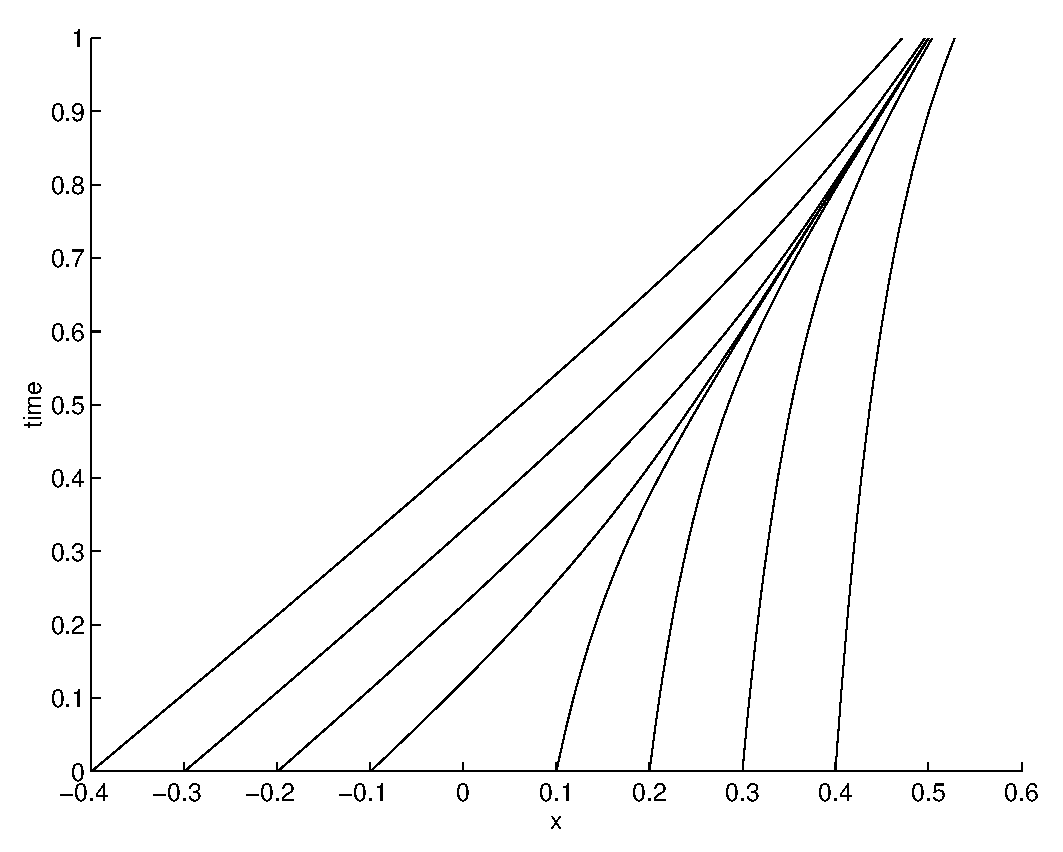
\psfig{figure=ambsthermopict/figCHARS.eps,height=2.5in,width=4in}}
\caption{Characteristics of the dual problem for a 
regularized shock solution.}
\end{figure}


As comparison, let us now attempt to derive a weak stability  estimate 
for (\ref{burgdual1}) in the case $u$ is a shock.
Multiplication 
by $\phi$ and integration over $Q_\tau$ gives
\[
\begin{array}{l}
 \frac{1}{2}\int_R
\phi^2(x,\tau )~dx + h\int_{Q_\tau}\left(
\phi^\prime (x,t)\right)^2~dxdt \vspace{3mm}\\
= -\frac{1}{2}\int_{Q_\tau}u^\prime 
\phi^2(x,t)~dx +\int_{R}e(x,t) \phi(x,t)~dx .
\end{array}\]
Since $u^\prime$ is large negative in the case of a shock, we have
large positive term of the right hand side, and using a Gronwall
inequality would results in a very large stability
factor. On the other hand, we show below weak stability for a 
rarefaction wave with $u^\prime\ge 0$, reflecting the 
above stability result for the perturbation equation.



Summing up, we see that for a shock, the linearized dual problem statisfies a strong
stability estimate with a stability factor of moderat size, while
a corresponding weak stability estimate appears to have a very large
stability factor. These stability features may be understood in a qualitative
sense, by pondering the directionality of the characteristics and the nature
of the $L_2$-norm. 

\section{Stability Estimates for a Rarefaction Wave}

We now consider the linearized dual Burgers' equation (\ref{burgdual1}),
linearized at the exact solution $u(x,t)=x/t$, corresponding to a rarefaction wave. 
Multiplying now (\ref{burgdual1}) by 
$-ht\phi^{\prime\prime}$, and using standard manipulations,
we obtain the following weighted norm strong stability estimate for $0<\tau <T$,
\begin{equation}\label{weightedstrongstab}
\Vert\tau^{1/2}h^{1/2}\phi^\prime\Vert 
+\Vert \omega h\phi^{\prime\prime}\Vert_{Q_\tau }
\leq \Vert \omega e\Vert_{Q_\tau } ,
\end{equation}
where $\omega (t)=t^{1/2}$ acts as a weight. 

A weighted norm analog of the a posteriori error estimate (\ref{apostburgers}) takes the form
\begin{equation}\label{weightedapostburger}
\Vert \omega^{-1} e\Vert_{Q_N}\le S_\omega\Vert \omega^{-1} hR(U)\Vert_{Q_N}
\end{equation}
with $S_\omega$ defined by the direct weighted norm analog of (\ref{stabburgers}).
The estimate (\ref{weightedstrongstab}) then shows that $S_\omega \sim 1$, 
and thus a rarefaction wave solution is computable in the weighted
norm with computational work corresponding to interpolation.
Note that the presence of the weight $t^{-1/2}$ will force more
stringent demands on the mesh for $t$ close to zero, which will
force an accurate resolution of the initial phase of the rarefaction.
This is intuitively reasonable and corresponds to the fact that an initial
error in the computation of a rarefaction will get amplified as time goes,
because characteristics diverge forward in time. On the other hand,
in the case of a shock, an initial error may be eliminated at later times,
because of converging characteristics, Thus, a rarefaction is more delicate
to compute than a shock, which we will see in the computational results 
we now present.





\section{Dual Solution and Stability Factors}

We display below RNS computations of a combination of  
a rarefaction wave and a shock using the cG(1)dG(0)-
method on a uniform space mesh with $h=10^{-3}$
and time step $10^{-4}$ taken from \cite{burman}.  We plot 
the computed solution at t=0,  t=0.3 , t=0.8, t=1 in Fig \ref{shockrarefaction}.
We see that the initial discontinuity
develops into a rarefaction and that a shock is formed for $t\approx 0.5$.

\begin{figure}[bhpt]
%\begin{center}

\includegraphics[height=4cm]{initburger}

\includegraphics[height=4cm]{03Tburger}

\includegraphics[height=4cm]{08Tburger}

\includegraphics[height=4cm]{Tburger}
\caption{A combined rarefaction and shock wave}
\label{shockrarefaction}
%\end{center}
\end{figure}


We solve the dual problem
using the following different approximations of the coefficient $a=(u+U)/2$
and the error $e$, with $\bar u$ the analytical, inviscid solution, 
and $U(h)$ the finite element solution on a mesh of size $h$:
(i) $a=(\bar u+U(h))$ and $e=\bar u-U(h)$,
(ii) $a=U(h)$ and $e=\bar u-U(h)$, (iii) $a=(U(h/4)+U(h))/2$ and $e=U(h/4)-U(h)$. 
We plot the corresponding dual solutions $\phi$ 
at the same time levels as above, but in revers
e order (t=1, t=0.8, t=0.3 , t=0)
in Fig \ref{dualsolution}.
\begin{figure}[bhpt]\label{dualsolution}
%\begin{center}

\includegraphics[height=4cm]{bdual10}

\includegraphics[height=4cm]{bdual08}

\includegraphics[height=4cm]{bdual03}

\includegraphics[height=4cm]{bdual00}
\caption{Dual solution in reverse time.}
%\end{center}
\end{figure}
We also plot in Fig. \ref{dualsol2} the corresponding second 
derivatives $\phi^{\prime\prime}$. 
\begin{figure}[bhpt]
%\begin{center}

\includegraphics[height=4cm]{bdualxx10}

\includegraphics[height=4cm]{bdualxx08}

\includegraphics[height=4cm]{bdualxx03}

\includegraphics[height=4cm]{bdualxx00}
\caption{Second deriatives of the dual solution in reverse time}
\label{dualsol2}
%\end{center}
\end{figure}
We note the change of $\vert\phi^{\prime\prime}\vert$, which may be viewed as a weight
in the a posteriori error estimate, from being 
large close to the shock at final time towards being large 
close to the initial discontinuity at $(x,t)=(0.2,0)$ initiating the rarefaction.
We see that that it is the data from the rarefaction at final time which
generates the large values of $\phi^{\prime\prime}$ at $t=0$, and not those
from the shock. This indicates that a rarefaction is more delicate to compute than a shock. 


We plot in Fig. \ref{stabfactorstrong} the strong stability factor $S$ defined
by (\ref{stabburgers})
for (i)-(iii) and $h=0.0001, \,h=0.00005, \,h=0.00001$.
\begin{figure}
%\begin{center}

\includegraphics[height=6cm]{S2veps}
\caption{Strong stability factor for different $h$}
\label{stabfactorstrong}
%\end{center}
\end{figure}
We see that $S\sim 1$, which shows that the Burgers' solution 
consisting of a rarefaction and shock wave is computable in 
$L_2(Q_N)$ with work comparable to interpolation.



\iffalse  % --- removed: placeholder section with missing figures (sphere/cylinder eps files not in repo) ---
\section{Turbulent Bluff Body Flow}
We show RNS flow with shocks around a sphere and cylinder in
Figs. \ref{sphere} and \ref{cyl}. This section will be
extended with turbulent/shock flow around a cube and sphere.
\begin{figure}[bhpt] 
\centerline{ 
\includegraphics[height=5.5cm]
{eps/3Dden.eps} 
\includegraphics[height=5.5cm]
{eps/3D_den_mach.eps} 
} 
\caption{Flow around a sphere}
\label{sphere} 
\end{figure}
\begin{figure}[bhpt] 
\centerline{ 
\includegraphics[height=10cm]
{eps/sphere_mesh.eps} 
} 
\caption{Mesh around a sphere}
\label{spheremesh} 
\end{figure}
\begin{figure}[bhpt] 
\centerline{ 
\includegraphics[height=5.5cm]
{eps/velocity_con.eps} 
\includegraphics[height=5.5cm]
{eps/velocity_con_2.eps}
} 
\caption{Section of 2d flow around a cylinder}
\label{cyl} 
\end{figure}

\section{Turbulent Flow in Heat Engines and Refrigerators}
This section will contain RNS simulations of diffuser flow with
gas expanding under cooling while getting heated by turbulence,
with the objective of computing losses and efficiency.
\fi  % --- end removed placeholder block (Bluff Body + Heat Engines stubs) ---

%\section{Transonic Flight}

%\section{Supersonic Flight}

\fi  % --- end moved Model Analysis block (Burgers + BurgersRNS moved to Appendix) ---













